\documentclass[a5paper]{book}

%%%%%%%%%%%%%%%%%%%%%%%%%%%%%%%%%%%%%%%%%%%%%%%%%
% Tungumál
%%%%%%%%%%%%%%%%%%%%%%%%%%%%%%%%%%%%%%%%%%%%%%%%%
%\usepackage[utf8]{inputenc}
\usepackage[icelandic]{babel}
\usepackage[T1]{fontenc} 

%%%%%%%%%%%%%%%%%%%%%%%%%%%%%%%%%%%%%%%%%%%%%%%%%
% Lykilatriði
%%%%%%%%%%%%%%%%%%%%%%%%%%%%%%%%%%%%%%%%%%%%%%%%%
\usepackage{latexsym}
\usepackage{comment} % fyrir debug!
\usepackage{amsmath,amssymb}  % amsthm

%%%%%%%%%%%%%%%%%%%%%%%%%%%%%%%%%%%%%%%%%%%%%%%%%
% Stærðfræði flýtiskipanir
%%%%%%%%%%%%%%%%%%%%%%%%%%%%%%%%%%%%%%%%%%%%%%%%%
\newcommand\bs{\char '134}   
\newcommand{\norm}[1]{\lVert#1\rVert}
\renewcommand{\vec}[1]{{\mbox{\boldmath$#1$}}}
\renewcommand{\theta}[1]{{\vartheta}}
\newcommand{\mat}[1]{{\mbox{\boldmath$#1$}}}
\newcommand{\reals}{{\mathbb R}}
\newcommand{\strng}[1]{{\mbox{\tt #1}}}
\newcommand{\inner}[2]{\big<\vec{#1}\cdot\vec{#2}\big>}
\def\argmax{\operatornamewithlimits{arg\,max}}

%%%%%%%%%%%%%%%%%%%%%%%%%%%%%%%%%%%%%%%%%%%%%%%%%
% Myndir og þess háttar
%%%%%%%%%%%%%%%%%%%%%%%%%%%%%%%%%%%%%%%%%%%%%%%%%
\usepackage[usenames,dvipsnames]{color}
\usepackage[]{graphicx,psfrag}
\usepackage{pstricks}
\usepackage{cancel}
\usepackage{rotating}

\usepackage{tikz}
\usetikzlibrary{positioning,calc}



%%%%%%%%%%%%%%%%%%%%%%%%%%%%%%%%%%%%%%%%%%%%%%%%%
% Hlekkir
%%%%%%%%%%%%%%%%%%%%%%%%%%%%%%%%%%%%%%%%%%%%%%%%%
\usepackage[colorlinks,linkcolor=black,citecolor=black,urlcolor=black]{hyperref}
%\usepackage[hyphenbreaks]{breakurl}

%%%%%%%%%%%%%%%%%%%%%%%%%%%%%%%%%%%%%%%%%%%%%%%%%
% Aðrar styttingar
%%%%%%%%%%%%%%%%%%%%%%%%%%%%%%%%%%%%%%%%%%%%%%%%%
\newcommand{\file}[1]{\texttt{#1}}


%%%%%%%%%%%%%%%%%%%%%%%%%%%%%%%%%%%%%%%%%%%%%%%%%
% Listings
%%%%%%%%%%%%%%%%%%%%%%%%%%%%%%%%%%%%%%%%%%%%%%%%%
\usepackage{listings}
\lstset{language=awk,
  basicstyle=\footnotesize,
  numbers=left,
  numberstyle=\footnotesize,
  numbersep=5pt,
  backgroundcolor=\color{white},
  showspaces=false,
  showstringspaces=false,
  showtabs=false,
  frame=single,
  tabsize=2,
  captionpos=b,
  breaklines=true,
  breakatwhitespace=false,
  title=\file{\lstname},
  commentstyle={\bf \color{green}}
}

%%%%%%%%%%%%%%%%%%%%%%%%%%%%%%%%%%%%%%%%%%%%%%%%%
% Aðrir pakkar
%%%%%%%%%%%%%%%%%%%%%%%%%%%%%%%%%%%%%%%%%%%%%%%%%
\usepackage{enumitem}
\usepackage{multirow}


%%%%%%%%%%%%%%%%%%%%%%%%%%%%%%%%%%%%%%%%%%%%%%%%%
% Glósu-flýtileiðir
%%%%%%%%%%%%%%%%%%%%%%%%%%%%%%%%%%%%%%%%%%%%%%%%%
\usepackage{framed}
\usepackage[thref,framed,amsmath]{ntheorem}


\theoremstyle{plain}% default
\newtheorem{thm}{Setning}[chapter]

\shadecolor{red}
\def\theoremframecommand{%
\psshadowbox[fillstyle=solid,fillcolor=lightgray,linecolor=black]}
\newshadedtheorem{setn}[section]{Setning}
\newshadedtheorem{hsetn}[section]{Hjálparsetning}
\newshadedtheorem{fsetn}[section]{Fylgisetning}
%\newtheorem{setn}{Setning}[chapter]
%\newtheorem{hsetn}[setn]{Hjálparsetning}
%\newtheorem{fsetn}[setn]{Fylgisetning}

\theoremstyle{plain}
%\theoremheaderfont{\normalfont\bfseries}\theorembodyfont{\slshape}
%\theoremsymbol{\ensuremath{\diamondsuit}}
%\theoremseparator{:}
\theorembodyfont{\upshape}
\theoremsymbol{\ensuremath{\ast}}
\theoremseparator{}
\newtheorem{daemi}{Dæmi}[chapter]


%%% ATHS

\theoremstyle{plain}
\theoremsymbol{\ensuremath{\clubsuit}}
\theoremseparator{.}
\theoremprework{\bigskip\hrule}
\theorempostwork{\hrule\bigskip}
\theoremheaderfont{\bfseries\slshape} % Slanted caps
\newtheorem*{aths}{Athugasemd}

%%%% Sönnun
\theoremstyle{nonumberplain}
\theoremheaderfont{\scshape} % Small caps
\theorembodyfont{\upshape} % Upright 
\theoremindent0cm
\theoremseparator{}
\theoremsymbol{\rule{1ex}{1ex}}
\newtheorem{proof}{Sönnun}

\theoremseparator{:}
\newtheorem{lausnSYND}{Lausn}
\theorembodyfont{\color{black}{\normalfont}}
\newtheorem{lausn}{Lausn}



\theoremclass{lausn}
\shadecolor{red}
\def\theoremframecommand{%
\psshadowbox[fillstyle=solid,fillcolor=lightgray,linecolor=black]}
\newshadedtheorem{flausn}[lausn]{Lausn}
\newshadedtheorem{yourpart}[lausn]{Your part}


%% Atriðisorðaskrá

\newcommand{\ath}[1]{{\bf{#1}}\index{#1}}
\newcommand{\athsub}[2]{{\bf{#1}}\index{#1!#2}}
\newcommand{\athsup}[2]{{\bf{#1}}\index{#2!#1}}

%% Kassar 


%----------------------------------------------------------------------------------------
%	TITLE PAGE
%----------------------------------------------------------------------------------------

\newcommand*{\titleGM}{\begingroup % Create the command for including the title 
%page in the document
    \hbox{ % Horizontal box
        \hspace*{0.2\textwidth} % Whitespace to the left of the title page
        \rule{1pt}{\textheight} % Vertical line
        \hspace*{0.05\textwidth} % Whitespace between the vertical line and 
        %title page text
        \parbox[b]{0.75\textwidth}{ % Paragraph box which restricts text to 
        %less than the width of the page
            
            {\noindent\Huge\bfseries \doctitleA \\[0.5\baselineskip] 
            \doctitleB}\\[2\baselineskip] % Title
            {\large \textit{\docsubtitle}}\\[4\baselineskip] % Tagline 
            %or further description
            {\Large \textsc{\docauthor}} % Author name
            
            \vspace{0.5\textheight} % Whitespace between the title block and 
            %the publisher
            {\noindent \publisher~\plogo}\\[\baselineskip] % Publisher and 
            %logo
        }}
        \endgroup}

\newcommand{\doctitleA}{Simplex \&}
\newcommand{\doctitleB}{sýningastúlkur}
\newcommand{\doctitle}{\doctitleA~\doctitleB}
\newcommand{\docsubtitle}{Inngangur að aðgerðagreiningu}
\newcommand{\docauthor}{Helga Ingimundardóttir}
\newcommand{\publisher}{GitHub}
\newcommand*{\plogo}{\fbox{$\mathcal{GH}$}} % Generic publisher logo

\usepackage[a5paper]{geometry}

%% sjá: ftp://ctan.tug.org/tex-archive/info/latex-samples/TitlePages/titlepages.pdf

\usepackage{lmodern}

\usepackage{url}

%\usepackage[svgnames]{xcolor}

%\usepackage{fontspec}

%\usepackage{graphicx}

%%\usepackage{hyperref}

%% drawing package

\usepackage{tikz}

%% for dingbats

\usepackage{pifont}

\providecommand{\HUGE}{\Huge}% if not using memoir

\newlength{\drop}% for my convenience

%% specify the Webomints family

%\newcommand*{\wb}[1]{\fontsize{#1}{#2}\usefont{U}{webo}{xl}{n}}

%% select a (FontSite) font by its font family ID

\newcommand*{\FSfont}[1]{\fontencoding{T1}\fontfamily{#1}\selectfont}

%% if you don’t have the FontSite fonts either \renewcommand*{\FSfont}[1]{}

%% or use your own choice of family.

%% select a (TeX Font) font by its font family ID

\newcommand*{\TXfont}[1]{\fontencoding{T1}\fontfamily{#1}\selectfont}

%% Generic publisher’s logo

\newcommand*{\plogo}{\fbox{$\mathcal{HI}$}}


%%%% Additional font series macros

\makeatletter

%%%% light series

%% e.g., kernel doc, section s: line 12 or thereabouts 
\DeclareRobustCommand\ltseries{\not@math@alphabet\ltseries\relax\fontseries\ltdefault\selectfont}

%% e.g., kernel doc, section t: line 32 or thereabouts

\newcommand{\ltdefault}{l}

%% e.g., kernel doc, section v: line 19 or thereabouts

\DeclareTextFontCommand{\textlt}{\ltseries}

% heavy(bold) series

\DeclareRobustCommand\hbseries{\not@math@alphabet\hbseries\relax\fontseries\hbdefault\selectfont}

\newcommand{\hbdefault}{hb}

\DeclareTextFontCommand{\texthb}{\hbseries}

\makeatother

\newcommand*{\titleGM}{\begingroup% Gentle Madness
\drop = 0.1\textheight
\vspace*{\baselineskip}
\vfill
\hbox{%
\hspace*{0.2\textwidth}%
\rule{1pt}{\textheight}
\hspace*{0.05\textwidth}%
\parbox[b]{0.75\textwidth}{
\vbox{%
\vspace{\drop}
{\noindent\HUGE\bfseries \doctitleA \\[0.5\baselineskip]
\doctitleB}\\[2\baselineskip]
{\Large\itshape \docsubtitle}\\[4\baselineskip] % undirtitill
{\Large \docauthor}\par
\vspace{0.5\textheight}
{\noindent Tæknigarður \the\year}\\[\baselineskip]
}% end of vbox
}% end of parbox
}% end of hbox
\vfill
\null
\endgroup}

\newcommand*{\titleSW}{\begingroup% Story of Writing

\raggedleft

\vspace*{\baselineskip}

{\Huge\itshape \doctitleA\\\doctitleB}\\[\baselineskip]

{\large\itshape \docsubtitle}\\[0.2\textheight]

{\Large \docauthor}\par

\vfill

{\Large \plogo{} \sffamily Tæknigarður \the\year}

\vspace*{\baselineskip}

\endgroup}

%\title{Aðgerðagreining}
%\author{Helga Ingimundardóttir}

\usepackage{fancyhdr}

\usepackage{makeidx}
\makeindex

\begin{document}

\pagestyle{empty}
%\titleSW 
\titleGM
\clearpage

\frontmatter

\chapter*{Um höfund}
\emph{Helga Ingimundardóttir} er doktorsnemi í tölvunarfræði við Háskóla Íslands. Helga kláraði B.Sc. gráðu í stærðfræði með hagnýttri tölvunarfræði frá Háskóla Íslands vorið 2008, jafnframt kláraði hún M.Sc. gráðu í reikniverkfræði frá sama skóla vorið 2010. 

Helga hefur kennt aðgerðagreiningu við Háskóla Íslands samhliða doktorsnáminu sínu undanfarin tvö vormisseri. Kennslubók þessi er unnin út frá fyrirlestrarnótum þeirra námskeiða og samstarfsverkefni við Matís, þar sem nemendur fengu tækifæri til að kynnast raunhæfum reikniverkefnum og hvernig mætti stilla þeim upp sem línulegum bestunarverkefnum og beita aðferðafræði úr aðgerðagreiningu við lausn þeirra. 

Kennslusýn Helgu er leiðsagnamiðað nám, þar sem áhersla er lögð á að nemendur 
fái að reyna við raunhæf verkefni og kynna sínar eigin lausnir. 

       % include preface

\tableofcontents

\mainmatter

\pagestyle{fancy}
\renewcommand{\chaptermark}[1]{\markboth{#1}{}}
\renewcommand{\sectionmark}[1]{\markright{\thesection\ #1}}
\fancyhf{}
\fancyhead[LE,RO]{\bfseries\thepage}
\fancyhead[LO]{\bfseries\rightmark}
\fancyhead[RE]{\bfseries\leftmark}
\renewcommand{\headrulewidth}{0.5pt}
\renewcommand{\footrulewidth}{0pt}
\addtolength{\headheight}{0.5pt}
\setlength{\footskip}{0in}
\renewcommand{\footruleskip}{0pt}
\fancypagestyle{plain}{%
\fancyhead{}
\renewcommand{\headrulewidth}{0pt}
}

\chapter{Inngangur}
\ath{Aðgerðagreining} eða aðgerðarannsóknir beinast að því að ákvarða hagkvæmustu leið til að framkvæma eitthvað innan fyrirtækja eða stofnana. Iðnaðarverkfræðingar fást oft slík rekstrar tengd verkefni, en aðgerðagreining takmarkast þó engan vegin við slík verkefni. 

Oft er um að ræða ákvarðanatöku þar sem flókin viðfangsefni eru sett fram sem bestunarverkefni. Lausn upphaflega verkefnisins felst þá í að finna hámark/lágmark á tilteknu falli, svokallað \ath{markfall}. 

Aðgerðagreining fellur undir hagnýta stærðfræði og samtvinnar m.a. tölfræði, líkindafræði, tölvunarfræði, ákvarðanafræði, biðraðafræði, leikjafræði, netafræði, hermun og bestun. Áherslan í þessari bók, verður mest lögð á líkanagerð og bestun. 

Aðgerðagreining eins og hún er stunduð í dag má rekja aftur til seinni heimstyrjaldarinnar þegar breskir og bandarískir vísindamenn voru fengnir til að finna hvernig ráðstafa mátti takmörkuðum auðlindum á hagkvæman máta. 

\section{Nokkur dæmi um bestunarverkefni} 
\begin{description} 
\item[Rekstur] Hámarka hagnað fyrirtækja (lágmarka skuldir?), hámarka afköst framleiðslulína, lágmarka kostnað við vörudreifingu (t.d. útkeyrslu og lagerhald). 
\item[Landbúnaður] Hámarka verðmæti uppskeru m.t.t. takmarkana á landrými, lágmarka kostnað við fóðurgjöf (t.d. kjúklinga eða svína). 
\item[Byggingarverkfræði] Lágmarka þyngd mannvirkja (t.d. háspennumöstur) sem uppfylla jafnframt hönnunarkröfur. 
\item[Umhverfisverkfræði] Koma mengun undir viðmiðunarmörk en lágmarka jafnframt kostnað við þær framkvæmdir. Hámarka hagnað af endur\-vinnslu. 
\item[Hagfræði] Hámarka þjóðarframleiðslu, taka þarf tillit til takmarkaðs vinnuafls, atvinnuleysis ofl. (Sjá t.d. \href{http://en.wikipedia.org/wiki/Wassily_Leontief}{Leontif}) 
\item[Fjarskiptaverkfræði] Bestun á úthlutun tíðnisviða í símkerfum. 
\item[Læknisfræði] Lágmarka skaða heilbrigðra líffæra í geislameðferð við krabba\-meini. 
\item[Fjármálaverkfræði] Val á hlutabréfum, lánastýring.
\end{description}

\begin{aths}Sjá fleiri tilvik um beitingu aðgerðagreiningar í töflu á bls. 4 í kennslubók. \end{aths}

\section{Ferli}

\begin{enumerate} 
\item Skilgreing verkefnis og gagnasöfnun. 
\item Stærðfræðilegt líkan útbúið sem fangar kjarna viðfangsefnisins. 
\item Tölvuforrit þróað til að vinna með líkanið. 
\item Prófun (sannreyning) líkans. Líkanið endurbætt ef nauðsyn krefur. 
\item Líkanið tekið í notkun -- yfirleitt í formi forrits. 
\end{enumerate} 
 
 
\chapter{Líkansmíð}
Stærðfræðilíkan: Líkir eftir þeim þáttum verkefnisins sem mestu máli skipta. 

\section{Ákvarðanataka} 
\begin{enumerate} 
\item Hvaða ákvarðanir þarf að taka? 
\item Hverjir eru valmöguleikarnir? 
\item Hver er árangurinn (ávinningurinn)? 
\item Hver eru skilyrðin fyrir góða ákvarðanatöku? 
\item Hvaða þættir hafa áhrif á ákvörðunartökuna? 
\item Hvernig getum við fullvissað okkur að hafa tekið rétta ákvörðun?  
\end{enumerate} 

\begin{daemi}[Gamalt prófdæmi]
Áður en bjór var leyfður á Íslandi var um 
tíma framleitt og selt svonefnt bjórlíki. Hugsum okkur að sá 
tími renni upp aftur og Ölgerðin þurfi að búa til bjórlíki með 
því að blanda saman pilsner (2.25\% alkóhól, kostar 100 kr. á 
lítra), vodka (40\% alkóhól, kostar 2000 kr. á lítra), brandíi 
(gefur gott bragð, 40\% alkóhól, kostar 3000 kr. á lítra) og 
maltöli (gefur bragð og lit, 1.5\% alkóhól, kostar 120 kr. á 
lítra). Til að líkið verði gott þarf 3-5\% að vera malt, a.m.k. 
2\% brandí, í mesta lagi 7\% vodki og sterkt vín mest vera 10\% 
samtals (annars kemur spírabragð). 
 
\begin{enumerate} 
\item Setjið fram línulegt bestunarverkefni fyrir uppskrift að 
  sem sterkustu (góðu) bjórlíki. 
\item Setjið fram slíkt verkefni fyrir uppskrift að sem ódýrustu 
  (en samt góðu) 4\% bjórlíki. 
\end{enumerate} 
\end{daemi}

\begin{lausn}
\begin{description}
  \item[Ákvarðanabreytur] $ P, V, B, M $ \quad (gefið í lítrum).
  \item[Styrkur] $2.25P+40V+40B+1.5M$ \quad (gefið í \%).
  \item[Skorður] $P\geq0,V\geq0,B\geq0,M\geq0$
  \begin{description}
  \item[Hlutfall]  $P+V+B+M=1$ 
  \item[Malt]	$\frac{3}{100}\leq M \leq \frac{5}{100}$
  \item[Brandí] $B\geq\frac{2}{100} $
  \item[Vodki] $V\leq\frac{7}{100}$
  \item[Sterkt] $V+B\leq\frac{10}{100}$
  \end{description}
\end{description}
\begin{enumerate}
  \item Markfall fyrir sterkasta og góðu bjórlíki er, $$\max_{P,V,B,M}~styrkur$$
  \item Markfall fyrir ódýrasta og 4\% bjórlíki er, $$\min_{P,V,B,M}~100P+2000V+3000B+120M$$ að viðbættri skorðu $styrkur=4$
\end{enumerate}

Besta lausn reynist vera:
\begin{center}
  \[\begin{array}{|lcc|c|}\hline & 1. & 2. &\\ \hline 
      P & 0.87 & 0.923 & \\
      V & 0.07 & 0.027 &\\
      B & 0.03 & 0.02 &\\
      M & 0.03 & 0.03 &\\ \hline \hline
    \mbox{styrkur}  & 6 & 4 & (\%)\\ \hline
    \mbox{kostn.} & 242.3 & 209.8 & (kr./\ell)\\ \hline
    \end{array}\]

\end{center}



\end{lausn}

\newpage 
\section{Stærðfræðilegt bestunarlíkan af verkefni}
\subsection{Helstu þættir}
\begin{itemize} 
\item Ákvörðunarbreytur (e. decision variables)  
\item Markfall (e. objective function)  
\item Skorður (e. constraints)  
\end{itemize} 

Víðtæka gagnasöfnun þarf til að meta stika (e. parameters) líkansins. 
Svokölluð næmnigreining er notuð til að meta áhrif breytinga í einstökum stikum líkansins. Ef í ljós kemur að líkanið er tiltölulega næmt fyrir gildum á einstökum stikum, þarf að vanda sérstaklega til við matið á þeim.
Slembin bestun (e. stochastic programming) tekur á óvissu í stikum líkansins með formlegum hætti.

\subsection{Tegundir líkana}
\begin{itemize}
 \item Ákvörðunarbreytur geta verið samfelldar (e. continuous), strjálar (e. discrete) eða hvoru tveggja.
 \item Markfall getur verið með eitt eða fleiri há-/lággildi.
 \item Skorður geta verið línulegar eða ólínulegar.
\end{itemize}

Aðaláherslan í námskeiðinu er á líkön með samfelldum breytum, línulegu markfalli og skorðum (línuleg bestun). Við munum að auki skoða svonefnda heiltölubestun (ákvarðanabreytur taka gildin $0,1,2,\ldots$).

Í grófum dráttum flokkast bestunarverkefni í eftirfarandi undirflokka:

\begin{itemize}
 \item Samfelldar ákvarðanabreytur (e. continuous) 
 \begin{itemize}
  \item Engar skorður (e. unconstrained)  
  \begin{itemize}
   \item Ólínulegar jöfnur 
   \item Aðferð minnstu fervika (e. least squares) 
   \item Víðvær bestun (e. global)
   \item Ekki diffranleg (e. non-differentiable)  
  \end{itemize}
  \item Skorðað (e. constrained)  
  \begin{itemize}
   \item {\bf Línuleg bestun} (e. linear programming)  
   \item Hálfákveðin bestun (e. semidefinite programming)
   \item Ólínulegar skorður (e. nonlinearly constrained)  
   \item Bundnar ákvarðanabreytur (e. bound constraints)  
   %\item Ferningsbestun
   \item {\bf Netbestun}
   \item Slembibestun (e. stochastic programming)
  \end{itemize}
 \end{itemize}
 \item Strjálar ákvarðanabreytur (e. discrete)  
 \begin{itemize}
  \item {\bf Heiltölubestun} 
  \item Slembibestun 
 \end{itemize}
\end{itemize}
Nemendur ættu að kannast við aðferð minnstu fervika úr Línulegri algebru (\href{https://ugla.hi.is/kennsluskra/index.php?tab=nam\&chapter=namskeid\&id=09101420106}{STÆ107G}). Áframhaldandi námskeið í aðgerðagreiningu eru til dæmis framhaldsnámskeiðin Slembin og víðvær bestun (\href{https://ugla.hi.is/kennsluskra/index.php?tab=nam\&chapter=namskeid\&id=08233620110}{IÐN201F}); Heiltölubestun, net\-líkön og röðun (\href{https://ugla.hi.is/kennsluskra/index.php?tab=nam\&chapter=namskeid\&id=08223820110}{IÐN201M}); og Ólínuleg bestun (\href{https://ugla.hi.is/kennsluskra/index.php?tab=nam\&chapter=namskeid\&id=08726820110}{REI202M}).

\section{Finna lausn út frá stærðfræðilegu líkani}
 
Hanna þarf sérhæft reiknirit (e. algorithm) fyrir hvert stærðfræðilegt líkan sem leitar (e. search) að bestu lausn (e. optimal solution). Sem dæmi, \emph{simplex aðferðin}: 
 
 
\href{http://en.wikipedia.org/wiki/George_Stigler}{Stigler} setur fram línulegt bestunarverkefni árið 1939 þar sem hann leitast við að lágmarka kostnað við að fæða fullorðinn karlmann en jafnframt uppfylla næringarþörf (RDS). Eftir nokkra yfirlegu fann Stigler lausn sem kostar $\$39.93$ á ári (m.t.t. verðbólgu væri núvirðið $\$561.43$). Hagkvæmast er að borða blöndu af heilhveiti, þurrmjólk, káli, spínati og baunum. Alla daga! 

Árið 1947 þróar George \href{http://en.wikipedia.org/wiki/George_Dantzig}{Dantzig} Simplex aðferðina fyrir línuleg bestunarverkefni. Besta lausn á verkefni Stigler reynist vera $\$39.69$ á ári (tók tvo mánuði að finna lausnina með handknúnum reiknivélum).

\begin{daemi}The Diet Problem: An Application of Linear Programming\newline\href
{http://www-neos.mcs.anl.gov/CaseStudies/dietpy/WebForms/index.html}{http://www-neos.mcs.anl.gov/CaseStudies/dietpy/WebForms/index.html}
\end{daemi}

Árið 1975 fá Leonid \href{http://en.wikipedia.org/wiki/Kantorovich}{Kantorovich} og Tjalling \href{http://en.wikipedia.org/wiki/Tjalling_Koopmans}{Koopmans} Nóbels verðlaun í hagfræði ``for their contribution to the theory of 
optimum allocation of resources'' (þ.e.a.s. línulega bestun). 
 \newpage
\begin{samepage}
\begin{daemi}[Gamalt prófdæmi] 
Jón ætlar að smíða pall við húsið sitt og er búinn að mæla út að hann þurfi eftirfarandi magn af $21\times95$ gagnvörðu pallaefni: 104 stk. 1.20m, 12 stk. 1.55m, 63 stk. 2.35m og 86 stk. 3.15 m. 
 
Hann ætlar að kaupa efnið í Húsasmiðjunni og þar fæst gagnvarið $21\times95$ í einni lengd, 3.90 m. Hve margar spýtur á hann að kaupa, og hvernig á að saga þær? 
\begin{samepage}
\begin{enumerate} 
\item Hvaða ákvarðanir þarf að taka? \\ (ákvörðunarbreytur $\vec{x}$) 
\item Hverjir eru valmöguleikarnir?  \\ ($\vec{x}\in X$) 
\item Hver er árangurinn (ávinningurinn?)? \\ (markfall $f(\vec{x})$) 
\item Hver eru skilyrðin fyrir góða ákvarðanatöku? \\ ($z=\max_\vec{x} f(\vec{x})$) 
\item Hvaða þættir hafa áhrif á ákvörðunartökuna? \\  (skorður $g_j(\vec{x})\le0, j=1,\ldots,m$) 
\item Hvernig getum við fullvissað okkur að hafa tekið rétta ákvörðun? \\ (rétt líkan?)  
\end{enumerate} 
\end{samepage}
\end{daemi}
\end{samepage}
\begin{lausn}Setjum þær upplýsingar sem okkur er gefið í töflu:
\[ \begin{array}{|c|c|}\hline \mbox{Fjöldi} & \mbox{Lengd} \\ \hline 
  104 & 1.20 \\
  12  & 1.55 \\
  63  & 2.35 \\
  86  & 3.15 \\ \hline 
\end{array}\]
Ákvarðanabreytur eru:
\[\begin{array}{clcl}
  x_1 & \mbox{fj. spýta í }3.15 &
  x_2 & \mbox{fj. spýta í }2.35+1.55 \\
  x_3 & \mbox{fj. spýta í }2.35+1.20 &
  x_4 & \mbox{fj. spýta í }1.55+1.55 \\
  x_5 & \mbox{fj. spýta í }1.55+1.20 \quad\quad&
  x_6 & \mbox{fj. spýta í }1.20+1.20+1.20
\end{array}\]
Markfallið okkar er 
$$ \min_{\vec{x}} z=\sum_{i=1}^6 x_i $$
m.t.t. skorðanna
\begin{eqnarray*}
  x_1 &\geq& 86 \\
  x_2+x_3 &\geq& 63 \\
  x_2+2x_4+x_5 &\geq& 12 \\
  x_3+x_5+3x_6 &\geq& 104 \\
  x_i &\geq& 0 \quad i\in\{1,..,6\}\\
  x_i && \textrm{heiltölur}
\end{eqnarray*}
Hér er stærðfræðilegt líkan komið á vandamálið, því er síðan hægt að leysa með aðferðum síðar kynnt í námskeiðinu. 
Besta lausn reynist vera
\[\begin{array}{ll}
    x_1^* = 86 & x_2^*=13 \\
    x_3^* = 50 & x_4^*= 0 \\
    x_5^* = 0  & x_6^*=18 \\
  \end{array}\]
með markfallsgildið $z^*=167$.


\end{lausn}


\begin{daemi}[Geislameðferð við krabbameini]\label{daemi:krabbi:grafisk}
Jónandi geislun er notuð til þess að drepa krabbameinsfrumur. Geislun veldur einnig skaða á heilbrigðum vef. Viljum lágmarka hann. Líffæri, bein og vefir dempa og dreifa geislun.

Höfum tvær tegundir geisla. Ákvarðanabreyturnar eru skammtastærð (mæld í kílórad) á hverjum geisla. 

G.r.f. að gleypni svæðis er í réttu hlutfalli af styrk geisla við viðborð, þá fundust eftir ítarlegar rannsóknir og útreikninga 
eftirfarandi hönnunar\-forsendur:

\begin{center}{\renewcommand{\arraystretch}{1.5} \renewcommand{\tabcolsep}{0.2cm}
\begin{tabular}{|l|rrr|}\hline
& \multicolumn{2}{c}{Gleypni svæðis} & \\
& Geisli 1 & Geisli 2 & Geislaskammtur \\\hline
Heildarmagn geislunar & 0.4 & 0.5 & lágmarka \\ 
Heilbrigðir vefir & 0.3 & 0.1 & $\leq 2.7 $ \\
Krabbameinssvæði & 0.5 & 0.5 & $=  6.0 $ \\
Miðja æxlis & 0.6 & 0.4 & $\ge 6.0$ \\ \hline
\end{tabular}} 
\end{center}

\end{daemi}
\begin{samepage}
\begin{lausn}Línulegt bestunarlíkan er því 
\begin{center}{\renewcommand{\arraystretch}{1.5} \renewcommand{\tabcolsep}{0.2cm}
\begin{tabular}{|l|rrr|}\hline
Heildarmagn geislunar & \multicolumn{3}{c|}{$\min_{x_1,x_2} z = 0.4x_1 + 0.5x_2$} \\ \hline
Heilbrigðir vefir & $0.3x_1$ & $+\; 0.1x_2$ & $ \le  2.7 $ \\
Krabbameinssvæði & $ 0.5x_1 $&$ +\; 0.5x_2 $&$=  6.0 $ \\
Miðja æxlis & $0.6x_1$&$ +\; 0.4x_2$& $\ge 6.0$ \\ 
& \multicolumn{3}{c|}{$x_1,x_2 \ge 0$} \\ \hline
\end{tabular}} 
\end{center}
\end{lausn}
\end{samepage}

\begin{aths}
Þar sem aðeins eru um tvær ákvarðanabreytur um að ræða er hægt að leysa líkanið grafískt. 
\end{aths}

\begin{figure}[h!]
\begin{center}
  \includegraphics[width=0.8\columnwidth]{figs/cancer.eps}
\end{center}\caption{Skorður vegna geislameðferðar}  
\end{figure}

\begin{samepage}
\begin{daemi}Banki nokkur vinnur að því að marka nýja útlánastefnu. Fjórar tegundir lána verða í boði:
\begin{center}{\renewcommand{\arraystretch}{1.5} \renewcommand{\tabcolsep}{0.2cm}
\begin{tabular}{|llcc|}\hline
& Tegund & Vextir & Afskrifarhlutfall \\ \hline
1 & Lán til fyrirtækja & $r_1$ & $p_1$ \\
2 & Lán til einstaklinga (neysla/yfirdráttur) & $r_2$ & $p_2$ \\
3 & Húsnæðislán & $r_3$ & $p_3$ \\
4 & Bílalán & $r_4$ & $p_4$ \\ \hline
\end{tabular}} 
\end{center} 
Hlutfallið sem þarf að afskrifa er metið út frá fyrri reynslu, og \mbox{$0<p_i<<1$}. 
Heildarfjármagn til ráðstöfunar er $L$ (t.d. í krónum). Jafnframt hefur eftirfarandi hefur verið ákveðið á síðasta stjórnarfundi:
\begin{itemize}
 \item A.m.k. 40\% af fjármagninu fer til fyrirtækja.
 \item Húsnæðislán a.m.k. helmingur bíla og neyslulána .
 \item Hámark 5\% heildarútlána sem þarf að afskrifa.
\end{itemize}
Ákvarða þarf hagkvæmustu ráðstöfun á fjármagni bankans.
\end{daemi}
\end{samepage}
\begin{lausn}
 Ákvarðanabreytur:
 $$ x_i = \textrm{ Fjármagn sem veitt er til lánaflokks } \quad i\in\{1,2,3,4\}$$
 Markfall
 $$ \max_{\vec{x}} z = \underbrace{\sum_{i=1}^4(1-p_i)r_ix_i}_{\textrm{tekjur af lánum}} - \underbrace{\sum_{i=1}^4 p_ix_i}_{\textrm{afskriftir}} $$
 því hlutfall í skilum fyrir lánaflokk $i$ er $1-p_i$ og vaxtatekjur þess eru $r_ix_i$.

 Skorðurnar eru 
{\renewcommand{\arraystretch}{1.5} \renewcommand{\tabcolsep}{0.2cm}
\[ \begin{array}{lrcl}
  \textrm{Heildarráðstöfun:}&\sum_{i=1}^4 x_i &\leq& L \\
  \textrm{Fyrirtæki:}&x_1 &\geq& 0.4 L \\
  \textrm{Einstaklingar:}&x_3 &\geq& \frac{1}{2} \left(x_4+x_2\right) \\
  \textrm{Hámarks afskriftir:}&\sum_{i=1}^4 p_ix_i &\leq& 0.05 \sum_{i=1}^4 x_i \\
  &x_1,x_2,x_3,x_4&\geq&0
 \end{array}\]}
\end{lausn}



 

\section{Hugbúnaður fyrir línulega bestun}
\subsection{Forrit sem leysa línuleg bestunarverkefni}
Forrit sem leysa línuleg bestunarverkefni eru t.d.

\begin{tabular}{ll}
 Excel &  $\div$ skelfilegt \\
 \href{http://www.mathworks.com/products/matlab/}{Matlab} & $\div$ rándýrt, $\div$ LP föll óþæginleg í notkun fyrir stór verkefni \\
 \href{http://www-01.ibm.com/software/integration/optimization/cplex-optimizer/}{CPLEX} & + mögulega það öflugasta sem er í boði, $\div$ rándýrt \\
 \href{http://www.mosek.com/}{MOSEK} & + öflugur pakki, + sanngjarnt verð \\
 \href{http://lpsolve.sourceforge.net/5.0/}{Ip-solve} & + ókeypis \\
 \href{http://www.gnu.org/software/glpk/}{GLPK} & + ókeypis \\
 \href{http://www.gurobi.com/}{gurobi} & + ókeypis stúdenta útgáfa \\
\end{tabular}

Fyrir Windows notendur er hægt að nota forritunarumhverfið \href{http://gusek.sourceforge.net/gusek.html}{GUSEK} fyrir GLPK.
 
\subsection{Líkindamál}
Svonefnd \ath{líkanamál} (e. modelling language) eru mjög gagnleg við að skilgreina stór bestunarverkefni. Dæmi um nokkur þeirra eru t.d.

\begin{tabular}{ll}
 MPL & + þæginlegt notendaviðmót, $\div$ selt \\
 GAMS & + rótgróið, $\div$ selt \\
 AMPL & + rótgróið, $\div$ selt \\
 MATHPROG & + einföld útgáfa af AMPL, + ókeypis 
\end{tabular}

\begin{aths}Í þessu námskeiði verður stuðst við GLPK og MATHPROG\end{aths}
\chapter{Almennt línulegt bestunarverkefni} 
Gerum ráð fyrir að eftirfarandi sé þekkt
\begin{itemize}
\item[$b_i$] Magn af hráefni (e. resources) með takmörkuðu framboði, til ráðstöfunar, þar sem \mbox{$i\in\{1,\ldots,m\}$}.
\item[$x_j$] Framleiðslumagn (e. activity) af afurð $j$, þar sem \mbox{$j\in\{1,\ldots,n\}$}.
\item[$c_j$] Framlegð af afurð $j$.
\item[$a_{ij}$] Magn af hráefni $i$ sem þarf til þess að framleiða afurð $j$.
\end{itemize}
Línulegt bestunarverkefni (LP) á \ath{stöðluðu} (e. standard) formi\footnote{Skv. Hillier og Lieberman} er að hámarka
\begin{equation}
\max_{x_1,\ldots,x_n}  z = \sum_{j=1}^n c_j x_j 
\end{equation}
með tilliti til skorðanna:
\begin{eqnarray}
\sum_{j=1}^n a_{ij} x_j  \le  b_i &\quad& i\in\{1,\ldots,m\} \\
x_j  \ge  0 &\quad&  j\in\{1,\ldots,n\}
\end{eqnarray}
eða á fylkjaformi:
\begin{equation}
 \max_{\mathbf{x}} z = \mathbf{c}^{T}\mathbf{x}
\end{equation}
með tilliti til skorðanna:
\begin{eqnarray}
\mathbf{A}\mathbf{x}  \le  \mathbf{b} \\
\mathbf{x} \ge  \mathbf{0}
\end{eqnarray}
\newpage
Önnur form LP verkefna eru einnig möguleg:
\begin{itemize}
 \item Lágmörkun, $\min_{\vec{x}} z$.
 \item Stærra-en skorður, $a_{i1}x_1+\cdots+1_{in}x_n\geq b_i$.
 \item Jafnt-og skorður,  $a_{i1}x_1+\cdots+1_{in}x_n = b_i$.
 \item Eitt eða fleiri $x_j$ geta verið neikvæð.
\end{itemize}
\begin{aths}
 Ólínulegum skorðum á forminu
$$ \frac{x_1}{x_2+x_3}\leq b$$
má breyta í jafngildar línulegar skorður
$$ x_1 \leq bx_2+bx_3 $$
eða
$$ x_1-bx_2-bx_3 \leq 0$$
Sjá sýnidæmi bls. 51-55 í H\&L.
\end{aths}

\begin{daemi}[Wyndor-Glass Company]\label{wyndor:org}
Wyndor glervöru\-framleiðandi ætlar að hefja framleiðslu á tveimur nýjum vörutegundum sem er hægt að framleiða þremur mismunandi verksmiðjum. 
\begin{itemize}
 \item Vara 1: Framleidd í verksmiðju 1 og 3
 \item Vara 2: Framleidd í verksmiðju 2 og 3
\end{itemize}
Hægt er að selja allt sem er framleitt. 
Eftirfarandi upplýsingar liggja fyrir:
\begin{center}{\renewcommand{\arraystretch}{1.5} \renewcommand{\tabcolsep}{0.2cm}
\begin{tabular}{|cccc|} \hline 
Verksmiðja & \multicolumn{2}{c}{Framleiðslutími (klst)} & Tími til umráðana \\
& Vara 1 & Vara 2 &  \\ \hline
1 & 1 & 0 & 4 \\
2 & 0 & 2 & 12 \\
3 & 3 & 2 & 18 \\ \hline 
Framlegð & \$3000 & \$5000 & \\ \hline
\end{tabular}

}\end{center}

Notum línulega bestun t.þ.a. ákvarða hversu mikið eigi að framleiða þannig að framlegðin sé hámörkuð.
\end{daemi}
\begin{lausn}Ákvarðanabreyturnar eru
\begin{eqnarray*}
 x_1 &=& \textrm{ magn af vöru } 1\\
x_2 &=& \textrm{ magn af vöru } 2
\end{eqnarray*}
Markfallið er 
\begin{equation}
\max_{x_1,x_2} 3x_1+5x_2 \label{wyndor:markfall} 
\end{equation}
m.t.t. skorðanna
\[\begin{array}{ccccc}
 x_1 & && \leq & 4 \\
 & &2x_2 & \leq &12 \\
 3x_1& + &2x_2&\leq&18\\
 &x_1,&x_2&\geq&0
\end{array}\]

Hér er einungis um tvær ákvarðanabreytur um að ræða, getum því fundið bestu lausn \emph{grafískt}. 
 
Viljum finna $\vec{x}^*=(x_1^*,x_2^*)$ sem hámarkar $z$. Fyrsta skrefið er að kanna hvaða gildi eru \emph{gjaldgeng} (e. feasible) þ.e. uppfylla allar skorður. Vitum að vegna þess að $x_1>0$ og $x_2>0$ þá kemur 1. fjórðungur eingungis til greina. Ytri mörk skorða (e. constraint boundary) fást m.þ.a. skipta ójöfnu út fyrir jöfnu. Til dæmis
$$ 3x_1+2x_2\leq 18 \quad \Rightarrow \quad 3x_1+2x_2=18$$
Í tveimur víddum eru þessi mörk línur.

\begin{aths}Til þess að finna hvorum megin við ytri mörkin gjaldgengar lausnir liggja, stingum við einhverjum heppilegum punkti, t.d. $(0,0)$ inn í ójöfununa og athugum hvort hún sé uppfyllt. 
\end{aths}
Því næst er að teikna hæðarlínur fyrir einhver gildi á $z$. Förum samsíða hæðalínunum í hækkandi átt (hér upp og til hægri) eins langt og kemst innan gjaldgegna svæðisins, ysti leyfilegi punkturinn er besta lausn líkansins. Sjáum á mynd \ref{wyndor:img:grafisk} að $\vec{x}^*=(2,6)$ gefur hæsta markfallsgildi, $z^*=36$.

\begin{figure}[t!]
\centering
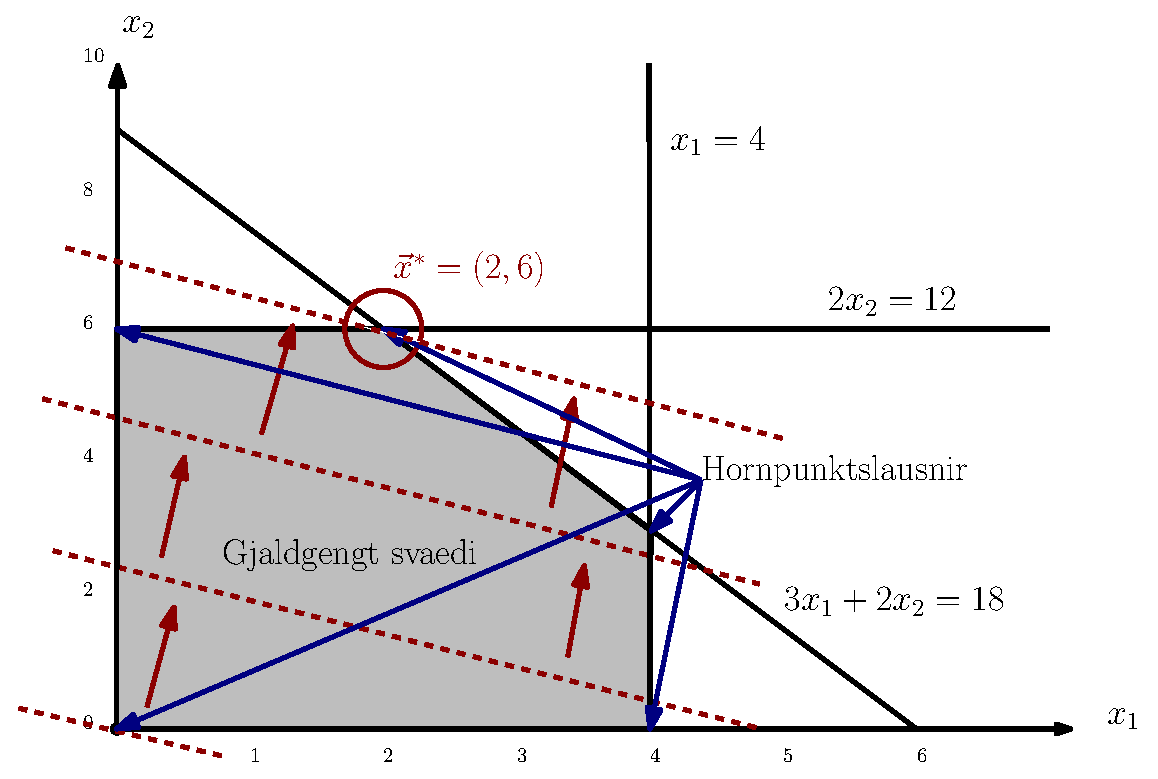
\includegraphics[width=0.7\columnwidth]{figs/wyndor_org.eps}
\caption{Myndræn lausn á dæmi \ref{wyndor:org} (Wyndor-Glass Company). Gjaldgegna svæðið afmarkast af skorðum líkansins, og hæðarlínur markfallsins $z$ eru teiknaðar sem rauðar brotalínur.}\label{wyndor:img:grafisk}
\end{figure}
\end{lausn}

\section{Nokkur hugtök}
%Til saman skilgreina skorðurnar \ath{gjaldgengt svæði} (e. feasible region) en það er mengi allra \ath{gjaldgengra lausna} (e. feasible solution).

%\ath{Besta lausn} (e. optimal solution) er sú lausn sem hámarkar (eða lágmarkar) markfallið $z$.

\begin{itemize}
\item \ath{Ákvarðanabreytur} (e. decision variables) $x_1,\ldots,x_n$
\item \ath{Ákvörðun eða lausn} (e. decision or solution) er tiltekin gildi á ákvarðana\-breytum
\item \ath{Markfall} (e. objective function) $z$
\item \ath{Gjaldgeng lausn} (e. feasible solution) er lausn sem uppfyllir skorður
\item \ath{Gjaldgengt svæði} (e. feasible region) mengi gjaldgengra lausna
\item \ath{Besta lausn} (e. optimal or best solution) er gjaldgeng lausn sem hámarkar (eða lágmarkar í $\min$  verkefni) markfall $z$
\begin{aths}
Stundum eru fleiri en ein jafngóðar bestu lausnir (jafnvel óendanlega margar, sbr. ef dæmi \ref{wyndor:org} væri með markfall samsíða skorðunni $z=3x_1+2x_2$).
\end{aths}
\item \ath{Gjaldgeng hornpunktslausn} (e. corner-point feasible solution) er lausn í hornpunkti gjaldgengs svæðis.
\end{itemize}

Lausn í hornpunkti gjaldgenga svæðisins er lausn þar sem $n$ ójöfnuskorður eru uppfylltar með $=$ merki; þær eru sagðar \athsup{virkar}{Skorður} (e. active).

Setja má fram bestunarverkefni sem hafa \ath{engar gjaldgengar lausnir} (e. infeasible).
\begin{daemi}\label{wyndor:infeasible}
Tökum dæmi \ref{wyndor:org} og bætum við skorðunni $$3x_1+5x_2\geq 50$$ þá eru skorðurnar sýndar myndrænt á mynd \ref{wyndor:img:infeasible}. Sjáum að við getum aldrei uppfyllt allar skorður samtímis, þ.a.l. engar gjaldgengar lausnir til á líkaninu.
\end{daemi}

\begin{aths}
 Þessi staða kemur stundum upp ef LP verkefni er sett ranglega fram.
\end{aths}

Annar möguleiki er að gjaldgegna svæðið sé \ath{ótakmarkað} (e. unbounded), þ.e.a.s. markfallið getur vaxið/minnkað hindrunarlaust.

\begin{daemi}\label{wyndor:unbounded}
Tökum aftur dæmi \ref{wyndor:org} og sleppum tveimur skorðum, þ.e.
$$\max_{\vec{x}}z=3x_1+5x_2$$
m.t.t. sk.
$$ x_1\leq 4$$
Sjáum á mynd \ref{wyndor:img:unbounded} að $z$ getur orðið eins stórt og vera vill.


\begin{figure}[t!]
\centering
\includegraphics[width=0.75\columnwidth]{figs/wyndor_infeasible.eps}
\caption{Myndræn lausn á dæmi \ref{wyndor:infeasible} (Wyndor-Glass Company). Gjald\-genga svæðið afmarkast af skorðum líkansins, sjáum að við getum aldrei uppfyllt allar skorður samtímis.}\label{wyndor:img:infeasible}
\includegraphics[width=0.75\columnwidth]{figs/wyndor_unbounded.eps}
\caption{Myndræn lausn á dæmi \ref{wyndor:unbounded} (Wyndor-Glass Company). Gjald\-genga svæðið afmarkast af skorðum líkansins, sjáum að $z$ getur orðið eins stórt og verða vill.}\label{wyndor:img:unbounded}
\end{figure} 
 
\end{daemi}

Athugum nú hvernig leysa má LP verkefni á skipulegan hátt. Eftirfarandi setning reynist gagnleg

\begin{setn}
Um línuleg bestunarverkefni með eina eða fleiri gjaldgengar lausnir og lausnarsvæði sem ekki eru ótakmörkuð gildir:
\begin{enumerate}
 \item Ef verkefnið hefur nákvæmlega eina bestu lausn, þá er hún í hornpunkti lausnarsvæðisins.
 \item Ef verkefnið hefur fleiri en eina bestu lausn þá eru a.m.k. tvær þeirra gjaldgengar hornpunktslausnir.
\end{enumerate}
\end{setn}
Fjöldi gjaldgengra hornpunktslausna er þar að auki endanlegur. 
Tillaga að reikniriti er því: 
Prófa allar gjaldgengar hornpunktslausnir.

\begin{aths}
 Í raunveruleikanum vex fjöldi slíkra punkta mjög hratt með fjölda ákvarðanabreyta $n$ og skorðna $m$, svo þetta reynist frekar óraunhæft reiknirit fyrir stærri verkefni.
\end{aths}


\section{Forsendur línulegrar bestunar}
Til þess að beita megi hefðbundinni línulegri bestun er gert ráð fyrir eftirfarandi forsendum:
\begin{description}
\item \ath{Hlutfallsleiki} (e. proportionality): Framlag afurðar $j$ til markfallsins er í hlutfalli við gildi á $x_j$, þ.e.a.s. $z$ er línulegt fall af ákvarðanabreytum. Sama gildir um vinstri hlið í skorðum. 
\item \ath{Samleggjanleiki} (e. additivity): Markfall og vinstri hlið skorða er summa framlaga frá einstökum afurðum.\footnote{
T.d. væri samlegðaráhrif nóg til að \emph{brjóta} þessa forsendu, sbr. \mbox{$z=3x_1+5x_2+x_1x_2$}}
\item \ath{Deilanleiki} (e. divisibility): Ákvarðanabreytur geta tekið hvaða rauntölugildi sem er innan lausnarsvæðisins.\footnote{
Ef þær þurfa að vera heiltölur þarf að nota heiltölubestun.}
\item \ath{Vissa} (e. certainty): Gerum ráð fyrir að gildi á \emph{stikum} $a_{ij}, b_i$ og $c_j$ séu að fullu þekkt (þ.e. ekki slembnir).
\end{description}


\chapter{Stöðlun verkefna} 
\lstset{language=matlab}
%\section{Verkefnum komið á staðlaða formið}

\section{Staðlað form}
Skv. H\&L er staðlað form eftirfarandi:
$$\max_{x_1,\ldots,x_n} \quad z = \sum_{j=1}^n c_j x_j  $$
m.t.t. sk.
\begin{eqnarray*}
\sum_{j=1}^n a_{ij} x_j  \le  b_i &\quad& i\in\{1,\ldots,m\}~~~~ (b_i \ge 0)\\
x_j  \ge  0, && j\in\{1,\ldots, n\}
\end{eqnarray*}
\section{Viðskeytt form}
$$\max_{x_1,\ldots,x_n}  z = \sum_{j=1}^n c_j x_j $$
m.t.t. sk.
\begin{eqnarray*}
\sum_{j=1}^n a_{ij} x_j  + x_{n+i} =  b_i &\quad& i\in\{1,\ldots,m\}~~~~ (b_i \ge 0)\\
x_j  \ge  0, && j\in\{1, \ldots, n+m\}
\end{eqnarray*}

\section{Önnur form línulegra bestunarvandamála}\label{Simplex:onnurform}
\subsection{Lágmörkunarverkefni}
Markfallið er 
$$\min_\vec{x}~~~z = \vec{c}^T\vec{x}$$
Því má breyta í jafngilt hámörkunarverkefni 
$$\max_\vec{x}~~~z = -\vec{c}^T\vec{x}$$

\subsection{Jöfnuskorður} 
$$\sum_{j=1}^n a_{ij} x_j =  b_i$$
Verkefni af þessu tagi er leyst með notkun \ath{gervibreytu} $\bar{x}$ (e. artificial variable). Þessi breyta lítur alveg eins út og slakabreyta nema henni er aðeins bætt við skorður sem innihalda jafnaðarmerki. Einnig er stuðullinn $-M$, sem hér táknar mjög stóra neikvæða tölu, margfaldaður með gervibreytunni í markfalli $z$ sem á að hámarka (til að refsa markfallinu).
Aðferðin kallast \ath{Aðferð stóra M} (e. big M method).

\begin{daemi}[Wyndor-Glass Company með jöfnuskorðu]\label{daemi:wyndor-jofnusk}
$$\max_{x_1,x_2}  z = 3x_1 + 5 x_2  $$
m.t.t. sk.
\begin{eqnarray*}
x_1 & \le&   4 \\
x_2 &\le&  12 \\
3x_1 + 2 x_2 & \color{red}{=} &   18 \\
x_1, x_2 &\ge& 0  
\end{eqnarray*}
\end{daemi}
\begin{lausn}[Viðskeytt \emph{big $M$ method}]
$$\max_{x_1,x_2,x_3,x_4,\bar{x}_5}  z = 3x_1 + 5 x_2 - M \bar{x}_5 $$
m.t.t. sk.
\begin{eqnarray*}
x_1 + x_3 & = &  4 \\
x_2 + x_4 & = & 12 \\
3x_1 + 2 x_2 + \bar{x}_5  & = &  18 \\
x_1, x_2, x_3, x_4, \bar{x}_5 &\ge &0   
\end{eqnarray*}
þar sem $M$ er stór tala. 

\begin{aths}
Ef hægt er að tryggja að í bestu lausn
viðskeytta verkefnisins sé $\bar{x}_5$ utan grunns (þ.e.
$\bar{x}_5=0$) þá gefur lausn þess okkur lausn á upphaflegu
verkefninu. Það er hægt með því að breyta markfallinu í $ z =
3x_1 + 5 x_2 - M \bar{x}_5$.  Hér er bætt við markfallið
$-M\bar{x}_5$ því um ræðir hámörkunarvandamál. Hins vegar ef um
lágmörkunarvandamál væri að ræða þá væri $+ M \bar{x}_5$ bætt
við markfallið. Það er hægt að líta á þetta eins og sé verið að
refsa markfallinu ef gervibreytan fær gildi $>0$.
\end{aths}
Byrjum á því að koma Simplex töflunni á eiginlegt form: þ.e.a.s. gervibreyta þarf að vera með $0$ í
grunni, þar sem allar gervibreytur byrja í grunni þarf að fjarlægja $M$ úr efstu röð (röð markfallsins) áður en
Simplex-aðferðin er beitt með hefðbundnum hætti.

\begin{center}
{\renewcommand{\arraystretch}{1.5} \renewcommand{\tabcolsep}{0.2cm}
{\scriptsize
$\begin{array}{|c|c|ccccc|c|l|} \hline 
\textrm{grunnbr.} &  Z &  x_1 &  x_2 &   x_3 &  x_4 &  \bar{x}_5 &  HH   & \textrm{min-ratio test}\\ 
\hline\hline \multicolumn{7}{l}{\textrm{Skref \#1 } >> T } \\ \hline
z   & 1 &-3 &-5 & 0 & 0 & \color{blue}{M} & 0 & \color{blue}{\textrm{koma á eiginlegt form}}\\
x_3 & 0 & 1 & 0 & 1 & 0 & 0 & 4 & \\
x_4 & 0 & 0 & 1 & 0 & 1 & 0 & 12 & \\
\bar{x}_5 & 0 & 3 & 2 & 0 & 0 & \fbox{1} & 18 & \color{blue}{\leftarrow \textrm{gervibr. úr }z}\\ \hline
\hline \multicolumn{7}{l}{\textrm{Skref \#2 } >> T=pivot(T,4,6) } \\ \hline
z   & 1 & \color{red}{-(3M+3)} & -(2M+5) & 0 & 0 & 0 & -18M & \color{red}{-3M << -2M}\\
x_3 & 0 & \fbox{1} & 0 & 1 & 0 & 0 & 4 & 4/1=4 \leftarrow \min \\ 
x_4 & 0 & 0 & 1 & 0 & 1 & 0 & 12 & -\\
\bar{x}_5 & 0 & 3 & 2 & 0 & 0 & 1 & 18 & 18/3=9\\ \hline
\hline \multicolumn{7}{l}{\textrm{Skref \#3 } >> T=pivot(T,2,2) } \\ \hline
z   & 1 & 0 & \color{red}{-(2M+5)} & 3M+3 & 0 & 0 & -6M+12 & \color{red}{\textrm{stærsta mínustala}}\\
x_1 & 0 & 1 & 0 & 1 & 0 & 0 & 4 &\\
x_4 & 0 & 0 & 1 & 0 & 1 & 0 & 12 & 12/1=12\\
\bar{x}_5 & 0 & 0 & \fbox{2} & -3 & 0 & 1 & 6 & 6/2=3\leftarrow \min\\ \hline
\hline \multicolumn{7}{l}{\textrm{Skref \#4 } >> T=pivot(T,4,3) } \\ \hline
z   & 1 & 0 & 0 &\color{red}{-4.5} & 0 & M+2 & 27 &\color{red}{\textrm{stærsta mínustala}}\\
x_1 & 0 & 1 & 0 & \fbox{1} & 0 & 0 & 4 & 4/1=4\leftarrow\min \\ 
x_4 & 0 & 0 & 0 & 1.5 & 1 & 0 & 9 & 9/1.5=6\\ 
x_2 & 0 & 0 & 1 &-1.5 & 0 & 0 & 3 &\\ \hline
\hline \multicolumn{7}{l}{\textrm{Skref \#5 } >> T=pivot(T,2,4)}\\ \hline
z   & 1 & 4 & 0 & 0 & 0 & M+2 & 45 & \color{red}{\textrm{engin mínustala}}\\
x_1 & 0 & 1 & 0 & 1 & 0 & 0 & 4 & \color{red}{\rightarrow \textrm{ besta lausn}}\\
x_3 & 0 &-1 & 0 & 0 & 1 & 0 & 3 &\\
x_2 & 0 & 1 & 1 & 0 & 0 & 0 & 9 &\\ \hline
\end{array}$}}
\end{center}
Hér má lesa úr lokatöflunni:
$$\vec{x} = (0,~ 9,~ 4,~ 3,~ 0)$$
eða
$$x_1^* = 0 \mbox{ og } x_2^* = 9 \mbox{~~~~~(besta lausn) }$$

Í skrefi \#1 erum við koma fylkinu yfir á eiginlegt form, því til að \mbox{geta} notað gervibreytuna $\bar{x}_5$ sem grunnbreytu þá þarf að losna við hana úr markfallinu. Restin af skorðunum haldast óbreyttar.

Í skrefum \#2 og \#3 er lausnin eingöngu gjaldgeng í breytta verkefninu, því $\bar{x}_5$ er enn í grunni, en í skrefum \#4 og \#5 eru lausnirnar gjaldgengar í upphaflega verkefninu.
\end{lausn}

\begin{aths}\hspace{.1cm}
\begin{itemize}
\item Ef allar gervibreytur eru jafnar núlli í bestu lausn þá
  höfum við fundið bestu lausn upprunalega vandamálsins.
\item Ef einhverjar gervibreytur eru enn í grunni þegar komið er
  í bestu lausn þá er það til marks um að upphaflega verkefnið
  hafi enga gjaldgenga lausn (munið að ``ekki grunnbreytur'' eru $0$
  og grunnbreytur eru fundnar með því að leysa jöfnunar).
  Tilgangur gervibreytu er eingöngu að fá fram upphafslausn.
\end{itemize} 
\end{aths}


Athugum nú hvernig væri hægt að nota innbyggða línulega bestunarfallið í \textsc{Matlab}\footnote{Ólíkt því sem gert er ráð fyrir í H\&L, þá er staðlað form línulegra bestunarverkefna í \textsc{matlab} lágmörkunarvandamál -- í stað hámörkunar.}, nefnilega \texttt{linprog}. Skoðum fyrst hjálpina:
\begin{lstlisting}
>> help linprog
 LINPROG Linear programming.
    X = LINPROG(f,A,b) attempts to solve the linear programming problem:
         
             min f'*x    subject to:   A*x <= b 
              x
 
    X = LINPROG(f,A,b,Aeq,beq) solves the problem above while additionally
    satisfying the equality constraints Aeq*x = beq.
\end{lstlisting}

\begin{lausn}[Dæmi \ref{daemi:wyndor-jofnusk} með \textsc{matlab}]Hægt er að láta \textsc{Matlab} styðjast við Simplex aðferðina í útreikningum sínum á eftirfarandi hátt:
\begin{lstlisting}
>> % Segja linprog ad nota simplex (ma sleppa)
>> options = optimset('linprog');
>> options.LargeScale = 'off';
>> options.Simplex = 'on';
>> % Wyndor verkefnid
>>  A = [1 0;0 1];b = [4;12];c = [3 5];Aeq = [3 2];beq = 18;
>> [x,fmax]=linprog(-c',A,b,Aeq,beq,[0 0]',[],[],options)
Optimization terminated.

x =
    0.0000
    9.0000

fmax =
  -45.0000 
\end{lstlisting}
Sem er eins og vænta mátti út frá niðurstöðu Stóru $M$ aðferðarinnar.
\end{lausn} 


\subsection{Stærri-en skorður með neikvæða hægri hlið}
Ef við höfum $\ge$ skorður  með  $b_i \le 0$, þá margföldum í gegn með $-1$, og fáum jafngilda $\le$ skorður með $b_i\ge0$. 

\begin{daemi}
$$2x_1+3x_2\ge -5 \quad \Leftrightarrow \quad -2x_1-3x_2\le 5$$ 
\end{daemi}

\subsection{Stærri-en skorður með jákvæða hægri hlið}
Ef við höfum $\ge$ skorður með  $b_i > 0$.

Byrjum á að setja inn slakabreytu $x_s$ eða \ath{umframbreytu} (e. surplus variable), til dæmis:

\begin{daemi}
$$2x_1 + 3x_2\ge 5 $$
\end{daemi}
\begin{lausn}Innleiðum umframbreytu á eftirfarandi hátt
$$\quad \Rightarrow \quad 2x_1 + 3x_2 - x_s =  5 \quad \textrm{og}\quad x_s\ge 0$$
Það þarf meira til, því ef við byrjum í $x_1=x_2=0$ (eins og venjulega) þá fæst $x_s=-5$, sem er ekki gjaldgengt. Þess vegna
bætum við nú líka við gervibreytu $\bar{x}$: 
$$2x_1 + 3x_2 - x_s + \bar{x} =  5$$ 
og  $x_s,\bar{x}\ge 0$ og bætum loks $-M\bar{x}$ við markfallið ($M$-aðferð). 
\end{lausn}

\subsection{Neikvæð gildi á ákvarðanabreytum}
\subsubsection{Neðri mörk}
Höfum neðri mörk á ákvarðanabreytu $x_j$, þ.e.
$$ x_j\geq L$$
þar sem $L$ er einhver neikvæður fasti.

\begin{lausn}
Skilgreinum $x_j'=x_j-L$, þá er $x_j'\geq0$. Stingum inn $(x_j'+L)$ alls staðar þar sem $x_j$ kemur fyrir, þ.e. í bæði skorðum og markfalli bestunarverkefnisins. 
\end{lausn}

\subsubsection{Engin neðri mörk}
Höfum engin neðri mörk á ákvarðanabreytu $x_j$, þ.e. $x_j\to-\infty$.
\begin{lausn}
Skilgreinum $x_j = x_j^+ - x_j^-$ með $x_j^+\geq0$ og $x_j^-\geq0$. Stingum inn $(x_j^+-x_j^-)$ alls staðar þar sem $x_j$ kemur fyrir, þ.e. í bæði skorðum og markfalli bestunarverkefnisins.
\end{lausn}

\begin{daemi}
$$\max_{x_1,x_2}  z = x_1 + x_2     $$
m.t.t. sk.
\begin{eqnarray*}
x_1 + 2x_2 & \le &  3 \\
3x_1 + x_2 &\le & 1 \\
-x_1 + x_2 &\le & 2 \\
x_2 &\ge& 0   
\end{eqnarray*}
 
\end{daemi}
\begin{lausn}Set $x=x^+-x^-$, og þ.a.l.
$$\max_{x^+,x^-,x_2} z = x^+-x^- + x_2     $$
m.t.t. sk.
\begin{eqnarray*}
x^+-x^- + 2x_2 & \le & 3 \\
3(x^+-x^-) + x_2 &\le&  1 \\
-(x^+-x^-) + x_2 &\le & 2 \\
x^+,x^-,x_2 &\ge& 0   
\end{eqnarray*}
 
\end{lausn}


\section{Tveggja fasa Simplex}
Stóra-$M$ aðferðin finnur fyrst lausn sem er gjaldgeng í upphaflega verkefninu (allar gervibreytur $=0$) og síðan tekur við leit að bestu lausn. 
\ath{Tveggja fasa aðferðin} (e. two phase method) gerir það sama -- án þess að innleiða stóra $M$. Í raun öðruvísi lýsing á stóru-$M$ aðferðinni. 

\begin{description}
  \item[Stóra $M$-aðferð] Lágmarka $z=0.4x_1+0.5x_2+M\bar{x}_4+M\bar{x}_6$
 \item[Tveggja fasa aðferð]\hspace{.1cm}
\begin{description}
 \item[Fasi 1] Lágmarka $z=\bar{x}_4+\bar{x}_6$ þangað til $\bar{x}_4=\bar{x}_6=0$ m.t.t. upprunanlegu skorðanna. Finnum bestu lausn fyrir gerviverkefnið, sem er gjaldgegn lausn fyrir raunverulega verkefnið.
 \item[Fasi 2] Lágmarka $z=0.4x_1+0.5x_2$ með $\bar{x}_4=\bar{x}_6=0$. Byrjum út frá bestu lausninni fengna úr Fasa 1. Getum sleppt dálkum sem tilheyra gervibreytum (þeir eru hvort eð er 0). Simplex-aðferð beitt til að leysa raunverulega verkefnið.
\end{description}
\end{description}

\begin{aths}
Ef engin gjaldgeng lausn er til á upphaflega verkefninu þá er lokalausn í fasa \#1 (eða stóru-$M$ aðferðinni) með að minnsta kosti eina gervi\-breytu $>0$.
\end{aths}

\newpage 
\begin{daemi}[Geislameðferð -- frh. af dæmi \ref{daemi:krabbi:grafisk}]\label{daemi:krabbi}

Höfum ákvarðanabreyturnar
\begin{itemize}
 \item[$x_1$] geislamagn fyrir geisla af tegund 1 
 \item[$x_2$] geislamagn fyrir geisla af tegund 2
\end{itemize}
og línulega bestunarlíkan sett fram með eftirfarandi hætti:

\begin{center}{\renewcommand{\arraystretch}{1.5} \renewcommand{\tabcolsep}{0.2cm}
\begin{tabular}{|l|rrr|}\hline
Heildarmagn geislunar & \multicolumn{3}{c|}{$\min_{x_1,x_2} z = 0.4x_1 + 0.5x_2$} \\ \hline
Heilbrigðir vefir & $0.3x_1$ & $+\; 0.1x_2$ & $ \le  2.7 $ \\
Krabbameinssvæði & $ 0.5x_1 $&$ +\; 0.5x_2 $&$=  6.0 $ \\
Miðja æxlis & $0.6x_1$&$ +\; 0.4x_2$& $\ge 6.0$ \\ 
& \multicolumn{3}{c|}{$x_1,x_2 \ge 0$} \\ \hline
\end{tabular}} 
\end{center}
\end{daemi}
\begin{lausn}Byrjum á því að setja verkefnið fram á staðlað form, þ.e. jöfnuform og $\max$ verkefni með því að bæta við slaka breytu $x_3$ og umframbreytu $x_5$:
\begin{center}{\renewcommand{\arraystretch}{1.5} \renewcommand{\tabcolsep}{0.2cm}
\begin{tabular}{|l|rrrrr|}\hline
Heildarmagn geislunar & \multicolumn{5}{c|}{$\max_{x_1,x_2,x_3,x_5}  -z = -0.4x_1 - 0.5x_2$} \\ \hline
Heilbrigðir vefir & $0.3x_1$ & $+\; 0.1x_2$ & $+\; x_3$ & & $ =  2.7 $ \\
Krabbameinssvæði & $ 0.5x_1 $&$ +\; 0.5x_2 $&&&$=  6.0 $ \\
Miðja æxlis & $0.6x_1$&$ +\; 0.4x_2$&&$ -\; x_5$ &$= 6.0$ \\ 
& \multicolumn{5}{c|}{$x_1,x_2,x_3,x_5 \ge 0$} \\ \hline
\end{tabular}}
\end{center}
Bætum því næst við gervibreytum, þeirra hlutverk er að búa til leyfilega byrjunarlausn:
\begin{center}{\renewcommand{\arraystretch}{1.5} \renewcommand{\tabcolsep}{0.2cm}
\begin{tabular}{|rrrrrrr|}\hline
\multicolumn{7}{|c|}{$\max_{\vec{x}}  -z = -0.4x_1 - 0.5x_2 -M \bar{x}_4  -M \bar{x}_6$} \\ \hline
$0.3x_1$ & $+\; 0.1x_2$ & $+\; x_3$ & & & & $ =  2.7 $ \\
$ 0.5x_1 $&$ +\; 0.5x_2 $&&$+\;\bar{x}_4$&&&$=  6.0 $ \\
$0.6x_1$&$ +\; 0.4x_2$&&&$ -\; x_5$ &$+\;\bar{x}_6$&$= 6.0$ \\ 
\multicolumn{7}{|c|}{$x_1,x_2,x_3,\bar{x}_4,x_5,\bar{x}_6 \ge 0$} \\ \hline
\end{tabular}}
\end{center}
\newpage
Beitum nú tveggja fasa Simplex-aðferðinni.
\begin{description}
 \item[Fasi \#1] Hafið til hliðsjónar töflu \ref{daemi:krabbi:fasi1}
\begin{itemize}
 \item Fasi \#1 gengur út á að leysa
$$\min_{\vec{x}} z=\bar{x}_4+\bar{x}_6 \quad \Leftrightarrow \quad \max_{\vec{x}} -z=-\bar{x}_4-\bar{x}_6$$
 \item Sjáum á töflunni að til þess að $\bar{x}_4$ og $\bar{x}_6$ verði grunnbreytur þarf að losna við þær úr markfalli (fyrstu 2 ítranir), þ.e. koma töflunni yfir á eiginlegt form.
 \item Því næst tekur við hefðbundin Simplex-bestun\footnote{Hefðbundin Simplex-bestun: stærsti neikvæði stuðull segir til um vendidálk og min-ratio test segir til um vendilínu.}. 
 \item Fasi \#1 gengur út á að finna löglega upphafslausn á raunverulega verk\-efninu, en hún er $\vec{x}_v=(6,6,0.3,0,0,0)$.
\end{itemize} 
\item[Fasi \#2] Hafið til hliðsjónar töflu \ref{daemi:krabbi:fasi2}
\begin{itemize}
 \item Fasi \#2 gengur út á að leysa
$$\max_{\vec{x}} -z=-0.4x_1-0.6x_2\quad\textrm{með}\quad \bar{x}_4=\bar{x}_6=0$$ 
\item Fasi \#2 hefst á því að breyta lokatöflu fasa \#1 þannig að dálkar gervibreytanna $\bar{x}_4$ og $\bar{x}_6$ er eytt (þurfum ekki lengur á þeim að halda) og upphaflegum kostnaði $\vec{c}$ er bætt við í efstu línuna $(z)$, sem gefur upphafstöfluna fyrir fasa \#2. 
 \item Komum nú töflunni á eiginlegt form, því $x_1$ og $x_2$ eru grunnbreytur og þ.a.l. þurfa stuðlarnir í efstu línu að vera 0. 
 %Sjáum að í fyrstu tveimur skrefum fasa \#2 hefur engin bestun enn átt sér stað, heldur eingöngu umritað verkefnið þ.a. grunnbreytur koma ekki lengur fyrir í markfalli. 
 \item Því næst er Simplex-aðferðin leyst með hefðbundnum hætti. 
 \item Að lokum lesum við úr lokatöflunni að besta lausn fyrir upprunanlega verkefnið er $\vec{x}^*=(x_1^*,x_2^*)=(7.5,4.5)$ með tilsvarandi markfallsgildi $z^*=5.25$.
\end{itemize}
\end{description}


\begin{center}
\begin{table}[t!]
{\renewcommand{\arraystretch}{1.5} \renewcommand{\tabcolsep}{0.2cm}
{\scriptsize
$$\begin{array}{|c|cccccc|c|l|} \hline 
 Z &  x_1 &  x_2 &   x_3 & \bar{x}_4 & x_5 &  \bar{x}_6 &  HH   & \textrm{min-ratio test}\\ 
\hline\hline \multicolumn{8}{l}{>> T1 } \\ \hline
-1.00 & \color{red}{0.00} & \color{red}{0.00} & 0.00 & \color{blue}{1.00} & 0.00 & \color{blue}{1.00} & 0.00 & \color{blue}{\textrm{koma á eiginlegt form}}\\
0.00 & 0.30 & 0.10 & 1.00 & 0.00 & 0.00 & 0.00 & 2.70 & \\
0.00 & 0.50 & 0.50 & 0.00 & \fbox{\color{blue}{1.00}} & 0.00 & 0.00 & 6.00 &\\
0.00 & 0.60 & 0.40 & 0.00 & 0.00 & -1.00 & \color{blue}{1.00} & 6.00 & \color{red}{\textrm{ath. engir $\vec{c}$ liðir í Fasa 1}}\\
\hline \multicolumn{8}{l}{>> T1=pivot(T1,3,5) } \\ \hline
-1.00 & -0.50 & -0.50 & 0.00 & 0.00 & 0.00 & \color{blue}{1.00} & -6.00 & \color{blue}{\textrm{koma á eiginlegt form}}\\
0.00 & 0.30 & 0.10 & 1.00 & 0.00 & 0.00 & 0.00 & 2.70 & \\
0.00 & 0.50 & 0.50 & 0.00 & 1.00 & 0.00 & 0.00 & 6.00 & \\
0.00 & 0.60 & 0.40 & 0.00 & 0.00 & -1.00 & \fbox{\color{blue}{1.00}} & 6.00 & \\
\hline \multicolumn{8}{l}{>> T1=pivot(T1,4,7) } \\ \hline
-1.00 & \color{red}{-1.10} & -0.90 & 0.00 & 0.00 & 1.00 & 0.00 & -12.00 & \color{red}{\textrm{stærsta mínustala}}\\
0.00 & 0.30 & 0.10 & 1.00 & 0.00 & 0.00 & 0.00 & 2.70 & 2.7/0.3=9\leftarrow \min \\
0.00 & 0.50 & 0.50 & 0.00 & 1.00 & 0.00 & 0.00 & 6.00 & 6/0.5=12\\
0.00 & 0.60 & 0.40 & 0.00 & 0.00 & -1.00 & 1.00 & 6.00 & 6/0.6=10\\
\hline \multicolumn{8}{l}{>> T1=pivot(T1,2,2) } \\ \hline
-1.00 & 0.00 & \color{red}{-0.53} & 3.67 & 0.00 & 1.00 & 0.00 & -2.10 & \color{red}{\textrm{stærsta mínustala}}\\
0.00 & 1.00 & 0.33 & 3.33 & 0.00 & 0.00 & 0.00 & 9.00 & 9/0.33=27\\
0.00 & 0.00 & 0.33 & -1.67 & 1.00 & 0.00 & 0.00 & 1.50 & 1.5/0.33=4.5\\
0.00 & 0.00 & \fbox{0.20} & -2.00 & 0.00 & -1.00 & 1.00 & 0.60 & 0.6/0.20=3\leftarrow \min \\
\hline \multicolumn{8}{l}{>> T1=pivot(T1,4,3)} \\ \hline
-1.00 & 0.00 & 0.00 & \color{red}{-1.67} & 0.00 & -1.67 & 2.67 & -0.50 & \color{red}{\textrm{stærsta mínustala}}\\
0.00 & 1.00 & 0.00 & 6.67 & 0.00 & 1.67 & -1.67 & 8.00 & 8/6.67=1.2 \\
0.00 & 0.00 & 0.00 & \fbox{1.67} & 1.00 & 1.67 & -1.67 & 0.50 & 0.5/1.67=0.3\leftarrow \min \\
0.00 & 0.00 & 1.00 & -10.00 & 0.00 & -5.00 & 5.00 & 3.00 & -\\
\hline \multicolumn{8}{l}{>> T1=pivot(T1,3,4)} \\ \hline
-1.00 & 0.00 & 0.00 & 0.00 & 1.00 & -0.00 & 1.00 & -0.00 & \color{red}{\textrm{engin mínustala}}\\
0.00 & 1.00 & 0.00 & 0.00 & -4.00 & -5.00 & 5.00 & 6.00 & \color{red}{\rightarrow \textrm{ besta lausn}}\\
0.00 & 0.00 & 0.00 & 1.00 & 0.60 & 1.00 & -1.00 & 0.30 & \color{blue}{\textrm{og }\bar{x}_4 \textrm{ og }\bar{x}_6\textrm{ eru}}\\
0.00 & 0.00 & 1.00 & 0.00 & 6.00 & 5.00 & -5.00 & 6.00 & \color{blue}{\textrm{komin úr grunni.}}\\
\hline
\end{array}$$}}
\caption{Fasi 1 fyrir dæmi \ref{daemi:krabbi}}\label{daemi:krabbi:fasi1}
\end{table}

\begin{table}[b!]
{\renewcommand{\arraystretch}{1.5} \renewcommand{\tabcolsep}{0.2cm}
{\scriptsize
$$\begin{array}{|c|cccc|c|l|} \hline 
 Z &  x_1 &  x_2 &   x_3 & x_5 &  HH   & \textrm{min-ratio test}\\ 
\hline\hline \multicolumn{6}{l}{>> T2 } \\ \hline
-1.00 & \color{blue}{0.40} & \color{blue}{0.50} & 0.00 & -0.00 & -0.00 & \color{blue}{\textrm{koma á eiginlegt form}}\\
0.00 & \fbox{1.00} & 0.00 & 0.00 & -5.00 & 6.00 & \\
0.00 & 0.00 & 0.00 & 1.00 & 1.00 & 0.30 & \\
0.00 & 0.00 & 1.00 & 0.00 & 5.00 & 6.00 & \\
\hline\hline\multicolumn{6}{l}{>> T2=pivot(T2,2,2)} \\ \hline 
-1.00 & 0.00 & \color{blue}{0.50} & 0.00 & 2.00 & -2.40 & \color{blue}{\textrm{koma á eiginlegt form}}\\
0.00 & 1.00 & 0.00 & 0.00 & -5.00 & 6.00 & \\
0.00 & 0.00 & 0.00 & 1.00 & 1.00 & 0.30 & \\
0.00 & 0.00 & \fbox{1.00} & 0.00 & 5.00 & 6.00 & \\
\hline\hline\multicolumn{6}{l}{>> T2=pivot(T2,4,3)} \\ \hline
-1.00 & 0.00 & 0.00 & 0.00 & \color{red}{-0.50} & -5.40 & \color{red}{\textrm{stærsta mínustala}}\\
0.00 & 1.00 & 0.00 & 0.00 & -5.00 & 6.00 & -\\
0.00 & 0.00 & 0.00 & 1.00 & \fbox{1.00} & 0.30 & 0.3/1=0.3\leftarrow\min\\
0.00 & 0.00 & 1.00 & 0.00 & 5.00 & 6.00 & 6/5=1.2\\
\hline\hline\multicolumn{6}{l}{>> T2=pivot(T2,3,5) } \\ \hline
-1.00 & 0.00 & 0.00 & 0.50 & 0.00 & -5.25 & \color{red}{\textrm{engin mínustala}}\\
0.00 & 1.00 & 0.00 & 5.00 & 0.00 & 7.50 & \color{red}{\rightarrow \textrm{ besta lausn}}\\
0.00 & 0.00 & 0.00 & 1.00 & 1.00 & 0.30 & \\ 
0.00 & 0.00 & 1.00 & -5.00 & 0.00 & 4.50 & \\ \hline\hline
\end{array}$$}}\caption{Fasi 2 fyrir dæmi \ref{daemi:krabbi}}\label{daemi:krabbi:fasi2}
\end{table}
\end{center}

\end{lausn}



\chapter{Simplex aðferðin}
\lstset{language=awk}

\section{Simplex-aðferðin}
Simplex-aðferðin er reiknirit (e. algorithm) sem notað er til þess að leysa línuleg bestunarverkefni.

Notum Wyndor-dæmið (\ref{wyndor:org}) til þess að kynnast aðferðinni
\begin{daemi}
$$\max_{x_1,x_2} z=3x_1+5x_2 $$
m.t.t. skorðanna
\[\begin{array}{ccccc}
 x_1 & && \leq & 4 \\
 & &2x_2 & \leq &12 \\
 3x_1& + &2x_2&\leq&18\\
 &x_1,&x_2&\geq&0
\end{array}\] 
\end{daemi}
Gjaldgegna svæðið er mengi allra punkta sem uppfylla skorðurnar (Sjá mynd \ref{wyndor:img:grafisk}). Ytri mörk skorðanna fást m.þ.a. skipta ójöfnu út fyrir jöfnu. Gjaldgengar hornpunktslausnir, GHL, liggja þar sem ytri mörk tveggja skorða mætast ($m$ skorður í almenna tilfellinu).

Tvær GHL eru sagðar \ath{aðlægar} (e. adjecent) ef þær deila saman einni skorðu ($m-1$ í almenna tilfellinu).

Notum eftirfarandi próf til þess að kanna hvort tiltekin GHL sé besta lausn (e. optimality test):
\begin{setn}[Optimality próf]
 Ef GHL-in hefur aðlægar GHL sem gefa hærra gildi á markfalli (lægra ef lágmörkun) þá er viðkomandi punktur besta lausn.
\end{setn}
\newpage
\subsection{Simplex-aðferðin í grófum dráttum}
\begin{enumerate}
 \item Finna einhverja GHL sem upphafslausn\footnote{Stundum má nota $\vec{0}=(0,\ldots,0)$.}
 \item Ef viðkomandi GHL er besta lausn, þá \emph{hætta}.\label{simplex:gróft}
 \item Færa sig yfir í betri GHL skv.
 \begin{enumerate}[label=(\roman{*})]
  \item Ferðast eftir þeirri skorðu sem gefur \emph{hröðustu aukningu} á markfalli.
  \item Stöðva þegar við rekumst á jaðar lausnarsvæðis.
  \item Finna nýjan punkt m.þ.a. finna skurðpunkt viðkomandi skorða.
 \end{enumerate}
 \item Aftur í skref \ref{simplex:gróft}.
\end{enumerate}

\begin{aths}
 Simplex-aðferðin var uppgötvuð 1947 af G. Dantzig. Hún er enn í fullu gildi -- helstu keppinautar eru innri punkts aðferðir (e. interior point method).
\end{aths}

\section{Viðskeytt form og grunnlausnir}
Gerum ráð fyrir að leysa skuli:
$$\max_{x_1,\ldots,x_n}  z = \sum_{j=1}^n c_j x_j  $$
m.t.t. sk. 
\begin{eqnarray*}
\sum_{j=1}^n a_{ij} x_j  \le  b_i & & i\in\{1,\ldots,m\}\\
x_j  \ge  0, &\quad & j\in\{1, \ldots, n\}
\end{eqnarray*}
þar sem $b_i \ge 0$.

Byrjum með gjaldgengu hornpunktslausninni
$$\vec{x}^{(0)} = \vec{0} \mbox{ þ.e. } x_1^{(0)}=x_1^{(0)}=\ldots=x_n^{(0)}=0$$

Í Simplex-aðferðinni erum við ítrekað að leysa jöfnur þegar farið er úr einni GHL í aðra. Til þess að auðvelda verkið breytum við öllum ójöfnu skorðum í jafnt-og skorður með því að innleiða \ath{slakabreytur} (e. slack variables).
 
Byrjum á að búa til \ath{viðskeytt} (e. augmented) verkefni með aðstoð \ath{slakabreyta} $x_{n+1},\ldots, x_{n+m}$:
$$ \max_{x_1,\ldots,x_n, x_{n+1},\ldots, x_{n+m}}  z = \sum_{j=1}^n c_j x_j  $$
m.t.t. sk.
\begin{eqnarray*}
\sum_{j=1}^n a_{ij} x_j + x_{n+i}  = b_i &\quad& i\in\{1,\ldots,m\}\\
x_k  \ge  0 &&  k\in\{1, \ldots, n+m\}
\end{eqnarray*}

Viðskeytta verkefnið er \emph{jafngilt} því upphaflega þannig að lausn á við\-skeytta verkefninu gefur lausn á upphaflegu verkefninu með því að sleppa slakabreytum. Á fylkjamáli er viðskeytta verkefnið:
$$\max_{\vec{x},\vec{x}_s}  z = \begin{bmatrix}\vec{c}^{T} 
  \vec{0}\end{bmatrix}\begin{bmatrix}\vec{x}\\\vec{x}_s\end{bmatrix}
  = \vec{c_v}^T\vec{x_v} $$
m.t.t. sk.
\begin{eqnarray*}
 \begin{bmatrix}\mat{A} &
  \mat{I}\end{bmatrix}\begin{bmatrix}\vec{x}\\ \vec{x}_s\end{bmatrix} = \mat{A_v}\vec{x_v}  &=&  \vec{b} \\
 \vec{x} \ge  \vec{0}, \vec{x}_s \ge  \vec{0} \mbox{ (eða) }
  \vec{x_v} &\ge& \vec{0}
\end{eqnarray*}
þar sem $\vec{x}$ eru ákvarðanabreytur upphaflega verkefnisins, $\vec{x}_s$ eru slaka\-breytur og $\vec{x}_v$ eru allar ákvarðanabreytur viðskeytta verkefnisins (þ.m.t. slakar).

\begin{daemi}
 Skorðan $x_1\leq4$ er jafngild $x_1+x_s=4$, $x_s\geq0$, þar sem $x_s$ segir til um hversu mikið $x_1$ getur vaxið til þess að skorðan sé bindandi.
\end{daemi}
%Þegar ójöfnuskorðum ($\leq$) hefur verið breytt á þennan hátt segjum við að verkefnið sé á \ath{viðskeyttu formi}.
\begin{daemi}[Wyndor verkefnið \ref{wyndor:org} á viðskeyttu formi]
$$ \max_{x_1,x_2}  z = 3x_1 + 5 x_2 $$
m.t.t. sk. 
\begin{eqnarray*}
 x_1+x_3 & =& 4 \\
 2 x_2 +x_4& =& 12 \\
 3x_1 + 2 x_2 +x_5& =& 18 \\
 x_1 , x_2, x_3,x_4,x_5 &\ge& 0
\end{eqnarray*}
þar sem $x_3,x_4,x_5$ eru slakabreyturnar.
\end{daemi}
\begin{aths}\hspace{.1cm}
 \begin{itemize}
  \item Ef slakabreyta $=0$ þá liggur punkturinn á jaðrinum
  \item Ef slakabreyta $>0$ þá liggur punkturinn innan gjaldgenga svæðisins
  \item Ef slakabreyta $<0$ þá liggur punkturinn utan gjaldgenga svæðisins
 \end{itemize}
\end{aths}


\subsection{Nokkur hugtök}

\begin{itemize}
 \item \ath{Viðskeytt lausn} (e. augmented solution): Gildi á ákvörðana\-breytum, ásamt tilsvarandi gildum á slakabreytum.\footnote{
 Lausnin $\vec{x}=(2,6)$ hefur tilsvarandi viðskeytta lausn \mbox{$\vec{x}_v=(2,6,1,8,5)$}.}
 \item \ath{Grunnlausn} (e. basic solution): Viðskeytt hornpunktslausn.
 \item \ath{Gjaldgeng grunnlausn} (e. basic feasible solution): Viðskeytt GHL.\footnote{
 Lausnin $\vec{x}=(0,6)$ er GHL, tilsvarandi viðskeytt GHL er \mbox{$\vec{x}_v=(0,6,4,0,6)$}.}
\end{itemize}
Fjöldi skorða á viðskeyttu formi er $m$ en fjöldi breyta er $n+m$ (vanákveðið jöfnuhneppi). Getum því valið hvaða gildi sem er á $n$ breytum og leyst fyrir þær sem eftir standa.

Í Simplex-aðferðinni eru þessar breytur settar $=0$ og þær eru sagðar \ath{utan grunns} (e. non-basic variable).
Breyturnar sem eftir standa og við leysum fyrir kallast \ath{grunnbreytur} (e. basic variables).
\begin{verbatim}
 
\end{verbatim}

\subsection*{Samantekt á eiginleikum grunnlausna}
\begin{itemize}
 \item Sérhver breyta er annaðhvort í grunni eða utan grunns.
 \item Fjöldi grunnbreyta er $=m$, fjöldi utan grunns eru $=n$ (og settar $=0)$.
 \item Gildi á grunnbreytum fást m.þ.a. leysa jöfnuhneppi sem samanstanda af skorðum viðskeytts verkefnisins.
 \item Ef grunnbreytur $\geq0$, þá er lausnin gjaldgeng grunnlausn.
\end{itemize}

\section{Algebruleg lausnaraðferð á dæmi}
\begin{daemi}[Lausn á Wyndor Glass Company í \ref{wyndor:org}]
$$ \max_{x_1,x_2}  z = 3x_1 + 5 x_2 $$
m.t.t. sk. 
\begin{eqnarray*}
 x_1 + x_3 & = &4 \\
 2x_2 + x_4 & = &12 \\
 3x_1 + 2x_2 + x_5 & = &18 \\
 x_1,x_2,x_3,x_4,x_5  &\ge& 0
\end{eqnarray*}
\end{daemi}
\begin{lausn}[Algebruleg lausnaraðferð]
\begin{verbatim}
 
\end{verbatim}

\begin{description}
\item[Skref 1] Hér er auðvelt\footnote{Ef við erum með $\le$ skorður og $b$-in eru $\ge 0$ (framboð á hráefni) þá gefur $\vec{x}=\vec{0}$ alltaf löglega lausn.} að finna gjaldgenga hornpunktslausn, setjum $x_1=0$ og $x_2=0$ (þ.e. utan grunns). Í grunni eru slakabreyturnar  með $x_3=4$, $x_4=12$ og $x_5=18$ (lesum beint af skorðunum). Byrjum því með gjaldgengu grunnlausnina $\vec{x}_v=(0,0,4,12,18)$.
 
 
\item[Skref 2] Best væri að framleiða eins mikið og mögulegt er á vöru $x_2$ (vegna þess að
  hagnaðurinn er $5$ og einungis $3$ fyrir vöru $x_1$). Veljum því $x_2$ inn í grunn.

Mesta aukningin fæst m.þ.a. fara eins langt og mögulegt er innan gjaldgenga svæðisins. Gætum að því að þegar $x_2$ vex, þá breytist gildi á öðrum breytum í grunni. Framleiðslan takmarkast af hráefni eða $x_2=6$ og þá þarf slakinn $x_4$ að fara úr $12$ niður í $0$:
\begin{eqnarray}
 x_1 + x_3 & = &4 \nonumber\\
 2 (6) + (0) & = &12 \label{eq:0}\\
 3x_1 + 2 (6) + x_5 & = &18 \nonumber 
\end{eqnarray}
umritum jöfnu \eqref{eq:0}
$$x_2 = \frac{12 - x_4 }{2}$$
og skipum út fyrir $x_2$ í öllum jöfnum og þá fáum við
$$\max_{x_1,x_2}  z = 3x_1 + 5 \frac{12 - x_4}{2} = 30 + 3x_1-\frac{5}{2} x_4$$
\begin{eqnarray*}
 x_1 + x_3 & = &4 \\
 \frac{2 x_2}{2} + \frac{x_4}{2} & = & \frac{12}{2} \\
 3x_1 + 2 \frac{12 - x_4 }{2} + x_5 & =&  18 
\end{eqnarray*}
eða
\begin{eqnarray*}
 x_1 + x_3 & = 4 \\
 x_2 + \frac{1}{2}x_4 & = 6\\
3 x_1-x_4+x_5 &= 6
\end{eqnarray*}
Endum með grunnlausnina $\vec{x}_v=(0,6,4,0,6)$
\item[Skref 3] 
$$\max_{x_1,x_2}  z =  30 + 3x_1-\frac{5}{2} x_4$$
m.t.t. sk.
\begin{eqnarray}
 x_1 + x_3 & = &4 \label{eq:1}\\
 x_2 + \frac{1}{2}x_4 & = &6 \label{eq:2}\\
 3x_1 -x_4 +x_5 & = &6 \label{eq:3}\\
 x_1, x_2, x_3, x_4, x_5 &\ge& 0 \nonumber
\end{eqnarray}
Nú má sjá að við getum grætt á því að framleiða vöru $x_1$
þar sem hagnaðurinn er $3$ en neikvæður fyrir $x_4$. Það mesta
sem við getum framleitt af $x_1$ er fyrir skorður:
\begin{description}
\item[\eqref{eq:1}] $x_1=4$ og $x_3$ lækkar niður í $0$.
\item[\eqref{eq:2}] engar hömlur á $x_1$.
\item[\eqref{eq:3}] $x_1=6/3=2$ og $x_5$ lækkar niður í $0$.
\end{description}
Mesta mögulega \emph{leyfilega} hækkun er því $x_1=2$ og $x_5=0$ (lækkar og fer þ.a.l. úr grunni fyrir $x_1$),
umritum skorðu \eqref{eq:3}:
$$x_1 = \frac{6 + x_4 - x_5}{3}$$
og skiptum út eins og áður:
\begin{eqnarray*}
\max_{x_1,x_2}  z  & = & 30+3\frac{6 + x_4 - x_5}{3} - \frac{5}{2}x_4 \\
 & =& 36-\frac{3}{2}x_4-x_5
\end{eqnarray*}
m.t.t. sk.
\begin{eqnarray*}
 \frac{6 + x_4 - x_5}{3} + x_3 & =& 4 \\
 x_2 + \frac{1}{2}x_4 & =& 6\\
 \frac{3x_1}{3} -\frac{x_4}{3} +\frac{x_5}{3} & = & \frac{6}{3}\\
 x_1, x_2, x_3, x_4, x_5 &\ge& 0 
\end{eqnarray*}
eða
\begin{eqnarray*}
 x_3+\frac{1}{3}x_4 - \frac{1}{3}x_5  & = &2 \\
 x_2 + \frac{1}{2}x_4 & =& 6\\
 x_1 -\frac{1}{3}x_4 +\frac{1}{3}x_5 & =& 2\\
 x_1, x_2, x_3, x_4, x_5 &\ge& 0 
\end{eqnarray*}
Endum með grunnlausnina $\vec{x}_v=(2,6,2,0,0)$
\item[Skref 4] Getum ekki aukið $z$ með því að velja $x_4>0$ eða $x_5>0$ (því stuðlarnir eru neikvæðir). Besta lausn er því fundin, og besta launin á \emph{upprunanlega} verkefninu er $\vec{x}^*=(x_1^*,x_2^*)=(2,6)$ með $z=36$.
\end{description}

\end{lausn}

\section{Simplex-aðferðin á töfluformi}
\ath{Simplex-taflan} er bókhald yfir framgangsmáta Simplex-aðferðarinnar. Hún heldur utan um stuðla í markfalli og skorðum.

Umritum jöfnurnar:
\setcounter{equation}{0}
\begin{eqnarray*}
\max_{x_1,\ldots,x_n} & z - \sum_{j=1}^n c_j
x_j = 0  & (0)\\
\mbox{m.t.t. sk.} & \sum_{j=1}^n a_{ij} x_j + x_{n+i} =  b_i
& (i)\\
\end{eqnarray*}
þar sem $i\in\{1,\ldots,m\}$ og komum þeim fyrir í Simplex-töflu, sjá Töflu \ref{table:simplex}.

\begin{table}[h!]\centering
{
\begin{tabular}{|c|c|c|ccc|ccc|c|}
\hline
grunn- & jafna & $z$ & $x_1$ & $\ldots$ & $x_n$ & $x_{n+1}$ &
$\ldots$ & $x_{n+m}$ & = hægri\\
breytur & & & &$\vec{x}$ & & & $\vec{x}_s$& & ~~~-hlið\\
\hline
 & (0) & $1$ &       & $-\vec{c}^T$ & & 0 & \ldots & 0 & 0 \\
\hline
$x_{1+n}$ & (1) & 0 & & & & & & & \\
$x_{2+n}$ & (2) & 0 & & & & & & & \\
 &  &  & & & & & & & \\
$\vdots$ & $\vdots$ & $\vdots$ & & $\mat{A}$ & & &$\mat{I}$ & & $\vec{b}$ \\
 &  &  & & & & & & & \\
$x_{m+n}$ & ($m$) & 0 & & & & & & & \\
\hline
\end{tabular}}
\caption{Simplex taflan $T$}\label{table:simplex}
\end{table}
 \newpage
\subsection{Aðgerðir á Simplex-töflu}
\begin{aths}G.r.f. að upphaflega verkefnið sé $\max \vec{c}^T\vec{x}$, með skorður $\mat{A}\vec{x}\leq\vec{b}$, $\vec{x}\geq\vec{0}$, og öll $b_i\geq0$. Önnur form LP verkefna eru tekin fyrir í grein \ref{Simplex:onnurform}).\end{aths}
\begin{description}
\item[Upphafsstilling] Koma verkefni yfir á viðskeytt form, slakabreytur í grunni.
 \item[Stoppskilyrði] Athuga hvort besta lausn sé fundin m.þ.a. skoða stuðla við ákvarðana\-breytur í markfalli (lína $(0)$). Ef allir stuðlar $\geq0$, þá er besta lausn fundin. {\bf Hætta}.\label{itrun:simplex}
\item[Finna nýja grunnbreytu] Sú breyta  með stærsta neikvæða stuðlinn í jöfnu (0) (\emph{stærsta} mínus tala í
 efstu línu) er valin, tilsvarandi dálkur kallast \ath{vendidálkur} ($j$). 
\item[Finna grunnbreytu sem fer út] með \emph{minimum ratio test}:
\begin{itemize}
 \item Deila tölum í hægri hlið ($b$-vigur) með tölum úr vendidálki (svo fremur sem þær eru $>0$, ef $=0$ þá sleppt).
 \item Línan með lægsta hlutfallið verður \ath{vendilína} ($i$). Tilsvarandi breyta fer úr grunni.
\end{itemize}
\item[Framkvæma Gauss-eyðingu] til að finna næsta punkt með því að marg\-falda línu með fasta $\neq0$, leggja saman/draga margfeldi einnar línu frá annarri, svokölluð ``elementary row operations''.
\item[Aftur] í stoppskilyrði.
\end{description}

\begin{aths}Ástæða Gauss-eyðingar: Höfum $n$ breytur utan grunns, allar $=0$, \mbox{leysum} $m\times n$ jöfnuhneppi t.þ.a. finna lausnina. Í hverju skrefi Simplex-aðferðarinnar kemur ein ný breyta í grunn og ein fer úr grunni. Gætum leyst jöfnuhneppi frá grunni, en það er óhagkvæmt. Þar sem lítið \mbox{hefur} breyst dugar nokkrar vel-valdar ``elementary row operations'' t.þ.a. finna lausn út frá þeirri gömlu.
 \end{aths}

\subsection*{MATLAB kóði}
\begin{lstlisting}
function T = pivot(T,i,j),
% usage: T = pivot(T,i,j);
  [m, n] = size(T);
  T(i,:) = T(i,:) / T(i,j);
  for k = 1:i-1, T(k,:) = T(k,:) - T(k,j) * T(i,:); end
  for k = i+1:m, T(k,:) = T(k,:) - T(k,j) * T(i,:); end
\end{lstlisting}


\begin{daemi}\label{wyndor:simplex}Beitum töflu-simplex aðferðinni á Wyndor-Glass Company:
\begin{equation}
 \max_{x_1,x_2}  z = 3x_1 + 5 x_2 \nonumber
\end{equation}
m.t.t. sk.
\begin{eqnarray}
 x_1  &\le& 4 \label{eq:4}\\ 
 2 x_2 & \le& 12 \label{eq:5}\\
 3x_1 + 2 x_2 & \le& 18 \label{eq:6}\\
 x_1, x_2 &\ge& 0 \nonumber
\end{eqnarray}
\end{daemi}
\begin{lausn}

Byrjum á því að setja fram líkanið á fylkjamáli:
$$ \max_{\begin{bmatrix}x_1 \\ x_2\end{bmatrix}} z = \begin{bmatrix}3 & 5 \end{bmatrix}\begin{bmatrix}x_1\\x_2\end{bmatrix} $$
m.t.t. sk.
\begin{eqnarray*}
 \begin{bmatrix}1 &  0\\0 & 2\\ 3 & 2\end{bmatrix}\begin{bmatrix}x_1 \\ x_2\end{bmatrix}  &\le&  \begin{bmatrix}4\\12\\18\end{bmatrix} \\
 \begin{bmatrix}x_1 \\ x_2\end{bmatrix} &\ge&  \begin{bmatrix}0 \\ 0\end{bmatrix}
\end{eqnarray*}
\newpage
Tilsvarandi Simplex-tafla er 
\begin{center}
{\renewcommand{\arraystretch}{1.5} \renewcommand{\tabcolsep}{0.2cm}
{\scriptsize
$\begin{array}{|c|ccccc|c|l|} \hline 
 Z &  x_1 &  x_2 &   x_3 &  x_4 &  x_5 &  HH   & \textrm{minratio-test}\\ 
\hline\hline \multicolumn{7}{l}{>> T } \\ \hline 
 1 & -3 & \bf{-5} &  0 &  0 &  0 &  0 & \\
 0 &  1 & 0 &  1 &  0 &  0 &  4 & - \\ 
 0 & 0 & \fbox{\bf{2}} &  0 &  1 &  0 & 12 & 12/2=6 \leftarrow \min \\
 0 &  3 & \bf{2} &  0 &  0 &  1 & 18 & 18/2=9 \\ 
\hline\hline \multicolumn{7}{l}{>> T = pivot(T,3,3)} \\ \hline 
 1 & \bf{-3} & 0 & 0 & \frac{5}{2} & 0 &  30 & \\
 0 & \bf{1} & 0 & 1 &   0 & 0 & 4 & 4/1=4\\
 0 & 0 & 1 & 0 & \frac{1}{2} & 0 & 6 & -\\
 0 & \fbox{\bf{3}} & 0 & 0 & -1 & 1 & 6 & 6/3=2 \leftarrow \min \\
\hline\hline \multicolumn{7}{l}{>> T = pivot(T,4,2)} \\ \hline 
 1 & 0 & 0 & 0 & \frac{3}{2} & 1 &  36 &\\
 0 & 0 & 0 & 1 & \frac{1}{3} & -\frac{1}{3} & 2 &\\
 0 & 0 & 1 & 0 & \frac{1}{2} & 0 & 6 & \\
 0 & 1 & 0 & 0 &  -\frac{1}{3} & \frac{1}{3} & 2 & \\ \hline \hline
\end{array}$
}}\end{center}

%\begin{figure}[b!]
%\centering
%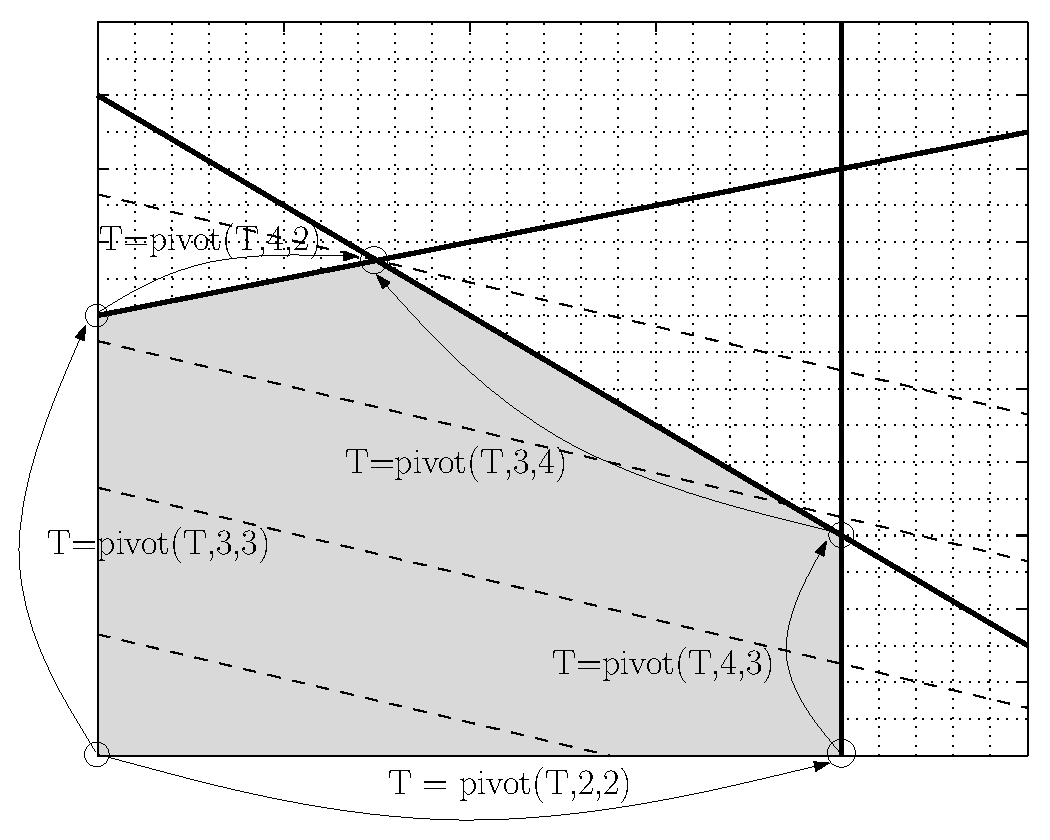
\includegraphics[width=0.9\columnwidth]{figs/daemi_simplex.eps}
%\caption{Rúmfræðileg skýring fyrir simplex-töflu í dæmi \ref{wyndor:simplex}}
%\end{figure}
 
Hér má lesa úr lokatöflunni:
$$\vec{x}_v = (2,~ 6,~ 2,~ 0,~ 0)$$
eða fyrir upprunanlega verkefnið
$$x_1^* = 2 \mbox{ og } x_2^* = 6 \mbox{~~~~~(besta lausn) }$$

Jafnframt er hægt að lesa úr fyrstu línu:
\begin{itemize}
 \item Besta gildi markfallsins: $z^*=36$,
 \item Skuggaverðin (e. shadow prices): $y_1^*, y_2^*, y_3^* = (0,~
\frac{3}{2}, ~ 1)$,
 \item Kostnaðarminnkun (e. reduced costs) fyrir $x_1$ og $x_2$ =
$(0, ~0)$.  
 \item Skorður \eqref{eq:5} og \eqref{eq:6} eru virkar vegna þess að slakabreyturnar $x_4$ og $x_5$ eru ekki grunnbreytur, þ.e.a.s. $x_4=x_5=0$.
\end{itemize}
\end{lausn}

\section{Hvað-ef greining}
Eftir að besta lausn hefur verið fundin er oft mjög gagnlegt að kanna áhrifa þess að breyta stikum líkansins. Slíkt kallast \ath{hvað-ef greining} (e. post\-optimality analysis).

%\subsection{Breytingar á \vec{b}}
Breytingar á hægri hlið skorðu $(i)$, t.d. ef $b_i$ hækkar um 1 þá getur það haft í för með sér breytingu á gildi markfallsins, $y_i=\frac{dz}{db_i}$ sem kallast \ath{skuggaverð} skorðunnar $(i)$.

\begin{daemi}[Hvað-ef greining Wyndor Glass Company]\label{wyndor:postoptimality}
$$\max_{x_1,x_2} z=3x_1+5x_2 $$
m.t.t. skorðanna
\begin{eqnarray}
 x_1 & \leq & 4 =: b_1 \label{postoptimality:1} \\ 
 2x_2 & \leq &12 =: b_2 \label{postoptimality:2} \\
 3x_1 + 2x_2&\leq&18 =: b_3 \label{postoptimality:3}
\end{eqnarray}
Hvaða áhrif hafa breytingar á $\vec{b}=(b_1,b_2,b_3)$ á markfallið?
\end{daemi}
\begin{lausn}
Leysum bestunarverkefnið myndrænt, mynd \ref{wyndor:img:postoptimality}. Sjáum að besta lausn er $\vec{x}^*=(2,6)$, með $z^*=36$.

Þar sem skorða \eqref{postoptimality:1} er ekki virk sjáum strax að ef $b_1$ hækkar um $1$ þá mun það ekki hafa áhrif á gildi markfallsins, því er skuggaverðið er $y_1=\frac{dz}{db_1}=0$.

Aftur á móti, er skorða \eqref{postoptimality:2} virk, svo ef við leyfum $b_2$ að hækka um 1 þá verður hún:
\begin{equation} 2x_2 \leq 13 \label{postoptimality:4}\end{equation}
Leysum nýja skurðpunktinn við skorður \eqref{postoptimality:3} og \eqref{postoptimality:4}, og fáum að nýja besta lausnin yrði $\vec{x}^*=(\frac{5}{3},\frac{13}{2})$ með $z^*=37.5$. Fáum því að breyting um $b_2$ um 1 hefur í för með sér breytingu á markfallinu um $\Delta z=\frac{3}{2}$, því er skuggaverðið er $y_2=\frac{dz}{db_2}=\frac{3}{2}$.

Eins fæst fyrir á breytingu $b_3$ úr 18 í 19 að nýja besta lausnin verður $\vec{x}^*=(\frac{7}{3},6)$ með $z^*=37$. Skuggaverðið er því $y_3=\frac{dz}{db_3}=1$.

\begin{figure}[h!]
\centering
\includegraphics[width=0.8\columnwidth]{figs/wyndor_postoptimality.eps}
\caption{Hvað-ef greining fyrir dæmi \ref{wyndor:postoptimality}}\label{wyndor:img:postoptimality}
\end{figure}
\end{lausn}

\newpage
\section{Samantekt um Simplex aðferðina}
 
\begin{description}
 \item[Z-röðin $(0)$]\begin{verbatim}\end{verbatim}
\begin{itemize}
\item Stuðlar breyta í grunni er alltaf núll.
\item Stuðlar breyta sem ekki eru í grunni geta verið $+$, $-$,
  eða $0$:
\begin{itemize}
\item ef $-$, þá getur breyta komið inn í grunn,
\item ef $+$, þá getur breyta ekki komið í grunn (ef allir stuðla $>0$ þá er
lausnin besta lausn),
\item ef $0$, breyta má koma inn í grunn, en það breytir ekki gildi
markfallsins (ef allir stuðlar eru jákvæðir og a.m.k. einn er núll þá eru
margar bestu lausnir á verkefninu).
\end{itemize}
\item Ef fleiri en ein breyta koma til greina sem næsta breyta í grunn (t.d. markfall $z=3x_1+3x_2$) þá skiptir ekki máli hver er valin.
\end{itemize}
\item[Víkjandi breyta]\begin{verbatim}\end{verbatim}
\begin{itemize}
\item Ef engin breyta getur farið út úr grunni (vendilína) þ.e.a.s. allir stuðlar í þeim vendidálki eru neikvæðir eða núll, þá er vandamálið \ath{ótakmarkað}\footnote{Líklega er villa í framsetningu á bestunarverkefninu, t.d. eina eða fleiri skorður vantar.} (e. unbounded)
\item Ef jafntefli í ``min-ratio'' próf milli tveggja breyta, þá er ein valin af handahófi.\footnote{Í þessu tilviki getur Simplex-aðferðin lent í vand\-ræðum, og farið í ``hringi''. En það kemur sjaldan fyrir í raunveruleikanum.}
\end{itemize}
\item[\ath{Skuggaverð}] (e. shadow price): $y_i = dz / db_i$.
  Skuggaverð fyrir skorðu $i$ mælir breytinguna á markfallinu
  ($z$) sem yrði ef $b_i$ væri aukin.
\item[\ath{Kostnaðarminnkun}] (e. reduced costs) er mesta leyfilega
  aukning í $c_j$ (ef $j$ er ekki grunn breyta) til að halda
  núverandi bestu gjaldgengu grunnlausn, eða m.ö.o. lágmarks hagnaður sem vara $j$ þarf að hækka um til að hún fari í grunn.
\end{description}
\begin{aths}
 Til eru fleiri afbrigði af Simplex-aðferðinni. Munurinn felst í að nota aðrar aðferðir til þess að velja breytu í og úr grunni.
\end{aths}

\section{Fræðin á bak við Simplex}
Til að meta hversu \emph{góð} Simplex-aðferðin er í raun og veru má dæma hana út frá hversu \emph{lengi} er Simplex-aðferðin að finna bestu lausn. Nokkar leiðir eru til að meta tímann sem það tekur að leita að bestu lausn, nefnilega
\begin{itemize}
 \item Tími (sek) -- hverfull skali þar sem ekki allar tölvur eru eins, og tölvur verða sífellt hraðvirkari.
 \item Fjöldi reikniaðgerða (samlagning, frádráttur, margföldun og deiling).
 \item Fjöldi ítrana -- í Simplex-aðferðinni er fjöldi reikniaðgerða í hverri ítrun ca. fasti (háður $m$ og $n$).
\end{itemize}
Greining á reikniritum miðast annaðhvort við \ath{versta tilvik} (e. worst case analysis) eða \ath{meðaltilvik} (e. average case).
Greining sem miðað við versta tilfelli skoðar öll verkefni af tiltekinni stærð ($m$ og $n$) og finnur hversu langan tíma erfiðasta tilvikið í hópnum tekur.

Þar sem Simplex-aðferðin fer aldrei til baka í eldri lausnir (nema í undantekninga tilvikum) þá er efra mark á fjölda gjaldgengra grunnlausna $$ \left(\begin{array}{c}n+m\\n\end{array}\right)=\frac{(m+n)!}{m!\;n!}$$
Fyrir $m=n$ gildir að 
$$ \frac{1}{2n}2^{2n}\leq \left(\begin{array}{c}2n\\n\end{array}\right) \leq 2^{2n} $$
þ.e. fjöldi hornpunkta vex \emph{mjög hratt} með $n$, t.d. $2^{50}\approx 1.1\cdot 10^{15}$.

Sýna má að verkefnið eftir Klee \& Minty\label{klee-minty} frá 1972\footnote{V. Klee and G.J. Minty. \emph{How Good is the Simplex Algorithm?} In O. Shisha, editor, Inequalities, III, pages 159–175. Academic Press, New York, NY, 1972}
$$ \max_{\vec{x}} z=\sum_{j=1}^n 10^{n-j} x_j $$
m.t.t. sk.
\begin{eqnarray*}
 2\sum_{j=1}^{i-1} 10^{i-j}x_j+x_i \leq 100^{i-1} &\quad& i\in\{1,...,n\} \\
 x_j\geq0 &\quad& j\in\{1,...,n\}
\end{eqnarray*}
tekur $2^n-1$ Simplex-ítranir. Reiknitími Simplex-aðferðarinnar (í versta tilfelli) vex því með veldisvísisfalli í $n$.

Á hinn boginn hafa menn séð að fyrir flest raunhæf verkefni er reiknitíminn miklu styttri. Eftirfarandi mat á fjölda ítrana fékkst með því að leysa 35 LP verkefni úr \href{http://www.netlib.org/}{\textsc{netlib}} safninu
$$ T\approx 0.5(n+m)^{1.05} $$
sem er fjarri versta tilvikinu.

\section{Simplex-aðferðin á fylkjaformi}
Línulegt bestunarverkefni á stöðluðu formi er 
$$\max_{\vec{x}} z=\vec{c}^T\vec{x}$$
m.t.t. sk.
\begin{eqnarray*}
 \mat{A}\vec{x}&\leq&\vec{b} \\ \vec{x}&\geq& \vec{0}
\end{eqnarray*}
þar sem $\mat{A}\in\mathbb{R}^{m\times n},\; \vec{c}\in\mathbb{R}^{n},\;\vec{x}\in\mathbb{R}^{n}$, og $\vec{b}\in\mathbb{R}^m$.

Komum verkefninu yfir á viðskeytt formi. Táknum slakabreytur með 
$$ \vec{x}_s = \begin{bmatrix}x_{n+1}\\ \vdots \\ x_{n+m} \end{bmatrix}$$
Skorðurnar verða þá
\begin{eqnarray*}
 \begin{bmatrix}\mat{A} & \mat{I}_m \end{bmatrix}\;\begin{bmatrix}\vec{x}\\\vec{x}_s \end{bmatrix}&=&\vec{b} \\
 \vec{x}_v=\begin{bmatrix}\vec{x}\\ \vec{x}_{s} \end{bmatrix}&\geq&\vec{0}
\end{eqnarray*}
þar sem $\mat{I}_m$ er $m\times m$ einingarfylki.

Fjöldi breyta utan grunns er $n$, setjum tilsvarandi breytur jafnar núlli. Höfum þá $m$ jöfnum með $m$ óþekktum breytum.

Táknum grunnbreyturnar með $\vec{x}_B$ og tilsvarandi dálkar úr $\begin{bmatrix}\mat{A} & \mat{I}_m\end{bmatrix}$ er fylkið $\mat{B}$ (þ.a. í upphafi er $\mat{B}=\mat{I}_m$). 
%\begin{aths} Röð dálka í $\mat{B}$ svara til röð staka í $\vec{x}_B$.\end{aths}
Höfum því $$ \mat{B}\vec{x}_B=\vec{b} $$
Lausnin er þá 
\begin{equation}
\vec{x}_B=\mat{B}^{-1}\vec{b} \label{eq:8} 
\end{equation}
\begin{aths}\hspace{.1cm}
\begin{itemize}
\item Getum séð hvernig lausnin breytist þegar $\vec{b}$ breytist lítið (sjá grein \ref{sec:naemnigreining} um næmnigreiningu)
\item Simplex-aðferðin velur breytur í og úr grunni þannig að tryggt er að $\mat{B}$ sé andhverfanlegt.
\item \ath{Endurskoðaða Simplex-aðferðin} (e. revised Simplex-method) í grein \ref{sec:revisedSimplex} reiknar andhverfuna á hagkvæman hátt.
\end{itemize} 
\end{aths}
Látum nú vigurinn $\vec{c}_B$ innihalda þá stuðla markfallsins sem svarar til breyta í $\vec{x}_B$ (önnur stök eru núll).
\begin{equation}
z=\vec{c}_B^T\vec{x}_B \stackrel{\eqref{eq:8}}{=}\vec{x}_B\mat{B}^{-1}\vec{b} \label{eq:9}
\end{equation}
Upphafsjöfnur Simplex-aðferðarinnar eru
\begin{equation}
 \begin{bmatrix}  1 & -\vec{c} & \vec{0} \\ \vec{0} & \mat{A} & \mat{I}_m \end{bmatrix} \; \begin{bmatrix} z \\ \vec{x} \\ \vec{x}_s \end{bmatrix} = \begin{bmatrix} 0 \\ \vec{b} \end{bmatrix} \label{eq:10}
\end{equation}
Í sérhverri ítrun gildir um \emph{hægri hlið} jöfnuhneppisins í \eqref{eq:10}.
\begin{equation}
 \begin{bmatrix}  z \\ \vec{x}_B \end{bmatrix}=\underbrace{\begin{bmatrix} 1 & \vec{c}_b\mat{B} \\ \vec{0} & \mat{B}^{-1}\end{bmatrix}}_{(\star)}\;\begin{bmatrix}0\\\vec{b}\end{bmatrix}=\begin{bmatrix} \vec{c}_B^T\mat{B}^{-1}\vec{b} \\ \mat{B}^{-1}\vec{b}\end{bmatrix}\quad\color{blue}{\begin{matrix} \leftarrow\eqref{eq:8} \\ \leftarrow\eqref{eq:9}\end{matrix}}
\end{equation}
Þar sem sömu aðgerðir $(\star)$ eru framkvæmdar á \emph{vinstri hlið} \eqref{eq:10} fæst
\begin{equation}
 \begin{bmatrix}1 & \vec{c}_B\mat{B}^{-1} \\ \vec{0} & \mat{B}^{-1} \end{bmatrix}\;\begin{bmatrix} 1 & -\vec{c} & \vec{0}  \\ \vec{0} & \mat{A} & \mat{I}_m \end{bmatrix} = \begin{bmatrix} 1 & -\vec{c}+\vec{c}_B\mat{B}^{-1}\mat{A}  & \vec{c}_B\mat{B}^{-1} \\ \vec{0} & \mat{B}^{-1}\mat{A} & \mat{B}^{-1}\end{bmatrix}
\end{equation}
Í sérhverri ítrun gildir því 
\begin{equation}
 \underbrace{\begin{bmatrix} 1 & -\vec{c}+\vec{c}_B\mat{B}^{-1}\mat{A}  & \vec{c}_B\mat{B}^{-1} \\ \vec{0} & \mat{B}^{-1}\mat{A} & \mat{B}^{-1}\end{bmatrix} }_{\textrm{vinstri hlið}}
 =\underbrace{\begin{bmatrix} \vec{c}_B^T\mat{B}^{-1}\vec{b} \\ \mat{B}^{-1}\vec{b}\end{bmatrix}}_{\textrm{hægri hlið}}
\end{equation}

\subsection{Fundamental insight}
Ef upphafstaflan er þekkt, þ.e.a.s.  $\mat{A},\;\vec{b}$ og $\vec{c}$, og ef $\mat{B}^{-1}$ í lokatöflu er þekkt, þá er hægt að reikna öll gildin í Simplex-töflunni með formúlunum hér að undan. Þetta er kallað \ath{fundamental insight}.

Jafnframt vitum við að í lokatöflu Simplex eru skuggaverðin $\vec{y}^*=\vec{c}_B\mat{B}^{-1}$.

\subsection{Samantekt}
\begin{center}
{\renewcommand{\arraystretch}{1.5} \renewcommand{\tabcolsep}{0.2cm}
{\footnotesize
\[ \begin{array}{|c|cc|c|cc|c|}\hline 
  \textrm{Simplex}& \textrm{Grunnbr.} & \textrm{Jafna} & z & \textrm{Upphafl. br.} & \textrm{Slakabr.} & \textrm{Hægri hlið} \\ \hline\hline
\textrm{Upphafstafla} & z & (0) & 1 & -\vec{c} & \vec{0} & 0 \\
(\textrm{Ítrun }0) &  \vec{x}_B & (1,\ldots,m) & \vec{0} & \mat{A} & \mat{I}_m & \vec{b} \\ \hline\hline
\vdots & \vdots & \vdots & \vdots & \vdots & \vdots & \vdots \\ \hline \hline
 & z & (0) & 1 & -\vec{c}+\vec{c}_B\mat{B}^{-1}\mat{A} & \vec{c}_B\mat{B}^{-1} & \vec{c}_B\mat{B}^{-1}\vec{b} \\
(\textrm{Ítrun }k) &  \vec{x}_B & (1,\ldots,m) & \vec{0} & \mat{B}^{-1}\mat{A} & \mat{B}^{-1} & \mat{B}^{-1}\vec{b} \\ \hline\hline
\vdots & \vdots & \vdots & \vdots & \vdots & \vdots & \vdots \\ \hline \hline
\textrm{Lokatafla} & z & (0) & 1 & -\vec{c}+\vec{y}^*\mat{A} & \vec{y}^* & \vec{y}^*\vec{b} \\
 &  \vec{x}_B & (1,\ldots,m) & \vec{0} & \mat{B}^{-1}\mat{A} & \mat{B}^{-1} & \mat{B}^{-1}\vec{b} \\ \hline
 \end{array}\]
}}
\end{center}
Í lok hverrar ítrunar segja stuðlar slakabreyta til um hvernig viðkomandi jöfnuhneppi fékkst út frá upphaflegu jöfnunum.

\begin{daemi}[Wyndor frh. af dæmi \ref{wyndor:simplex}]Upphafs- og lokatöflur eru:
\begin{center}
{\renewcommand{\arraystretch}{1.5} \renewcommand{\tabcolsep}{0.2cm}
{\footnotesize
\[ \begin{array}{|c|cc|c|cc|ccc|c|}\hline 
\textrm{Simplex}& \textrm{Grunnbr.} & \textrm{Jafna} & z & \multicolumn{2}{c|}{\textrm{Upphafl. br.}} & \multicolumn{3}{c|}{\textrm{Slakabr.}} & \textrm{Hægri hlið} \\ \hline\hline
\textrm{Upphafstafla} & z & (0) & 1 & -3 & -5 & 0 & 0& 0 & 0 \\ \hline
 &  x_3 & (1) & 0 & 1 & 0 & 1 & 0 & 0 & 4 \\
 &  x_4 & (2) & 0 & 0 & 2 & 0 & 1 & 0 & 12 \\ 
 &  x_5 & (3) & 0 & 3 & 2 & 0 & 0 & 1 & 18 \\ \hline\hline
\vdots & \vdots & \vdots & \vdots & \vdots & \vdots & \vdots & \vdots & \vdots & \vdots \\ \hline \hline
\textrm{Lokatafla} & z & (0) & 1 & 0 & 0 & {\color{blue}{0}} &{\color{blue}{\frac{3}{2}}} & {\color{blue}{1}} & 36\\ \hline
 &  x_3 & (1) & 0 & 0 & 0 & \color{red}{1} & \color{red}{\frac{1}{3}} & \color{red}{-\frac{1}{3}} & 2 \\
 &  x_2 & (2) & 0 & 0 & 1 & 0 & \frac{1}{2} &  0 & 6 \\ 
 &  x_1 & (3) & 0 & 1 & 0 & 0 & -\frac{1}{3} & \frac{1}{3} & 2 \\ \hline
 \end{array}\]
}}
\end{center} 
\end{daemi}
\begin{lausn}Sjáum að 
\begin{eqnarray*}
\textrm{Lína 1} &=& {\color{red}{1}} \cdot\textrm{(upphafl.lína 1)}+{\color{red}{\frac{1}{3}}}\cdot\textrm{(upphafl.lína 2)}{\color{red}{-\frac{1}{3}}}\cdot\textrm{(upphafl.lína 3)}\\
&=& 1\cdot\begin{bmatrix}1 & 0 \end{bmatrix}+\frac{1}{3}\cdot\begin{bmatrix}0 & 2\end{bmatrix}-\frac{1}{3}\cdot\begin{bmatrix}3 & 2\end{bmatrix} = \begin{bmatrix} 0 & 0\end{bmatrix} \\
\textrm{Lína 2} &=& 0\cdot\begin{bmatrix}1 & 0 \end{bmatrix}+\frac{1}{2}\cdot\begin{bmatrix}0 & 2\end{bmatrix}+0\cdot\begin{bmatrix}3 & 2\end{bmatrix} = \begin{bmatrix} 0 & 1\end{bmatrix} \\
\textrm{Lína 3} &=& 0\cdot\begin{bmatrix}1 & 0 \end{bmatrix}-\frac{1}{3}\cdot\begin{bmatrix}0 & 2\end{bmatrix}+\frac{1}{3}\cdot\begin{bmatrix}3 & 2\end{bmatrix} = \begin{bmatrix} 1 & 0\end{bmatrix} 
\end{eqnarray*}
Að auki fáum við innsýn í skuggaverðin $\vec{y}^*$ þar sem 
\begin{eqnarray*}
z^*&=&\vec{y}^*\vec{b}= \sum_{i=1}^m y_i^*b_i={\color{blue}{0}}\cdot4+{\color{blue}{\frac{3}{2}}}\cdot12+{\color{blue}{1}}\cdot18=36 
\end{eqnarray*}
 \end{lausn}

\subsection{Endurskoðuð Simplex-aðferð}\label{sec:revisedSimplex}
\ath{Endurskoðuð Simplex-aðferð} (e. revised Simplex-method) gengur út á að geyma aðeins $\mat{B}^{-1}$ geymt og því er breytt í hverri ítrun með formúlu sem er á bls. 185 í kennslubók. Í upphafi er $\mat{B}^{-1}=\mat{I}_m$. 
\newpage
\lstset{language=matlab}
\begin{daemi}[Wyndor í \textsc{matlab}]Höfum gefið
$$\mat{A}=\begin{bmatrix}1 & 0\\0 & 2\\3 & 2\end{bmatrix}, \quad \vec{b}=\begin{bmatrix}4\\12\\18\end{bmatrix},\quad\vec{c}=\begin{bmatrix}3\\5\end{bmatrix},\quad \mat{B}^{-1}=I_3$$ 
\end{daemi}
\begin{lausn}

%\begin{table}[h]
%\begin{minipage}[b]{0.5\linewidth}\centering
Til upprifjunar er hefðbundin Simplex-aðferð:
\begin{lstlisting}
>> A=[1 0;0 2;3 2];b=[4;12;18];c=[3 5]';[m,n]=size(A);I=eye(m);
>> T = [1 -c' zeros(1,m) 0 ; zeros(m,1) A I b]

T =

     1    -3    -5     0     0     0     0
     0     1     0     1     0     0     4
     0     0     2     0     1     0    12
     0     3     2     0     0     1    18

>> % Itrun #1 --------------------------------------------------
>> T=pivot(T,3,3) 

T =

    1   -3    0    0    2.5000    0   30
    0    1    0    1         0    0    4
    0    0    1    0    0.5000    0    6
    0    3    0    0   -1.0000    1    6

>> % Itrun #2 --------------------------------------------------
>> T=pivot(T,4,2) 

T =

    1    0    0    0    1.5000    1.0000   36
    0    0    0    1    0.3333   -0.3333    2
    0    0    1    0    0.5000         0    6
    0    1    0    0   -0.3333    0.3333    2
\end{lstlisting}
%\end{minipage}
%\hspace{0.5cm}
%\begin{minipage}[b]{0.5\linewidth}
Nú skulum við leysa verkefnið með endurskoðaðri Simplex-aðferð, skv. reikni\-riti í kennslubók á bls. 185:
\begin{lstlisting}
>> A=[1 0;0 2;3 2];b=[4;12;18];c=[3 5]';[m,n]=size(A);
>> c_B = [0 0 0]; % Framlegd vid grunnbreytur x3,x4,x5 er 0 
>> invB = eye(3); % I upphafi er invB=I_m
>> T = [1,           -c'+c_B*invB*A,  c_B*invB,  c_B*invB*b  
       zeros(m,1),  invB*A,          invB,      invB*b    ]

T =

     1    -3    -5     0     0     0     0
     0     1     0     1     0     0     4
     0     0     2     0     1     0    12
     0     3     2     0     0     1    18

>> % Itrun #1 --------------------------------------------------
>> k=2; % x2 entering basic
>> r=2; % x4 leaving basic
>> eta = -invB*A(:,k)/(invB(r,:)*A(:,k))

eta =

     0
    -1
    -1

>> eta(r)=1/(invB(r,:)*A(:,k))

eta =

         0
    0.5000
   -1.0000

>> E=I; E(:,r)=eta

E =

    1.0000         0         0
         0    0.5000         0
         0   -1.0000    1.0000

>> invB=E*invB % Uppfaersla a invB

invB =

    1.0000         0         0
         0    0.5000         0
         0   -1.0000    1.0000

>> c_B = [0 5 0], % Framlegd vid grunnbreytur x3,x2,x5 


>> T = [1,           -c'+c_B*invB*A,  c_B*invB,  c_B*invB*b  
       zeros(m,1),  invB*A,          invB,      invB*b    ]

T =

    1   -3    0    0    2.5    0   30
    0    1    0    1    0      0    4
    0    0    1    0    0.5    0    6
    0    3    0    0   -1      1    6


>> % Itrun #2 --------------------------------------------------
>> k=1; % x_1 entering basic
>> r=3; % x_5 leaving basic
>> eta = -invB*A(:,k)/(invB(r,:)*A(:,k)); 
>> eta(r)=1/(invB(r,:)*A(:,k)); E=I; E(:,r)=eta;
>> invB=E*invB % Uppfaersla a invB

invB =

    1.0000    0.3333   -0.3333
         0    0.5000         0
         0   -0.3333    0.3333

>> c_B = [0 5 3], % Framlegd vid grunnbreytur x3,x2,x1
>> T = [1,           -c'+c_B*invB*A,  c_B*invB,  c_B*invB*b  
       zeros(m,1),  invB*A,          invB,      invB*b    ]

T =

    1    0    0    0    1.5000    1.0000   36
    0    0    0    1    0.3333   -0.3333    2
    0    0    1    0    0.5000         0    6
    0    1    0    0   -0.3333    0.3333    2

>> % Skuggaverd, kostnadarminnkun, gildi markfalls og bestu lausn
>> ystar = c_B*invB, reduced_cost = ystar*A-c', z = ystar*b, xstar=zeros(n+m,1); xstar([3 2 1])=invB*b

ystar =

         0    1.5000    1.0000

reduced_cost =

     0     0

z =

    36

xstar =

     2
     6
     2
     0
     0
\end{lstlisting}
%\end{minipage}
%\end{table}

 
\end{lausn}






\chapter{Nykurverkefni} 
\lstset{language=awk}

Sérhverju línulegu bestunarverkefni má breyta í svokallað \ath{nykur} (e. dual) verkefni, sem er þá einnig línulegt bestunarverkefni. Einnig kalla \ath{gagnvirkt} verkefni. 

Verkefnin tengjast á þann hátt að lausn á einu verkefni gefur okkur lausnina á hinu. Skuggaverð í frumverkefninu eru ákvörðunarbreytur nykurverkefnisins og öfugt. Stundum er þægi\-legra og hagkvæmara að leysa tilsvarandi nykurverkefni heldur en upphaflega verkefnið.

Gjaldgeng lausn á öðru verkefninu gefur efri (neðri) mörk á bestu lausn hins verkefnisins. 

\begin{daemi}[Efri og neðri mörk]\label{daemi:efrinedrimork}
$$\max_{\vec{x}} z=4x_1+x_2+3x_3 $$
\begin{eqnarray}
x_1+4x_2&\leq&1\\ \label{sk:11}
3x_1-x_2+x_3&\leq&3\\ \label{sk:12}
x_1,x_2,x_3&\geq&0 \nonumber
\end{eqnarray}
\end{daemi}
\begin{lausn}
Ljóst er að sérhver gjaldgeng lausn gefur okkur \emph{neðri mörk} á bestu lausn, t.d. $\vec{x}=(1,0,0)$ gefur $z=4$. Með $\vec{x}=(0,0,3)$ fæst $z=9$. Er þetta seinna gildi nálægt því besta? Til þess að svara því reynum við að finna efri mörk á markfallið.

Margföldum \eqref{sk:11} með 2 og \eqref{sk:12} með 3 og leggjum þær saman (fastar fundnir með ``störun'')
\[\begin{array}{rrrrrrl}
  2(&x_1& +4x_2&& \leq & 1)\\
+ 3(&3x_1&-x_2&+x_3&\leq & 3)\\ \hline
 &  11x_1&+2x_2&+3x_3 &\leq &11
\end{array}\]
Þar sem allar breytur eru $\geq0$ gildir að
$$ \underbrace{4x_1+x_2+3x_3}_{\textrm{markfallið}} \quad \leq \quad \underbrace{11x_1+2x_2+3x_3 \leq 11}_{2\eqref{sk:11}+3\eqref{sk:12}}
$$
þ.e. besta lausn liggur á bilinu $9\leq z^*\leq 11$.

Hægt er að gera enn betur en þetta. Notum breyturnar $y_1$ og $y_2$ í stað fastanna 2 og 3 og finnum þau gildi sem gefa bestu efri mörk. 
\[\begin{array}{rrrrrrl}
  y_1(&x_1& +4x_2&& \leq & 1)\\
+ y_2(&3x_1&-x_2&+x_3&\leq & 3)\\ \hline
 &  (y_1+3y_2)x_1&+(4y_1-y_2)x_2&+(y_2)x_3 &\leq &1(y_1)+3(y_2)
\end{array}\]
Gerum kröfu  um að stuðlar við $x$-in séu a.m.k. jafnstórir og stuðlar markfallsins (svo mörkin haldi), 
\begin{eqnarray*}
 y_1+3y_2 &\geq& 4\\
 4y_1-y_2&\geq&1\\
y_2&\geq&3\\
y_1,y_2&\geq&0
\end{eqnarray*}
Berum nú markfallið saman við þessa summu (og efri mörk hennar)
\begin{eqnarray*}
 z&=&4x_1+x_2+3x_3\\&=&(y_1+3y_2)x_1+(4y_1-y_2)x_2+(y_2)x_3 \\ &\leq &\underbrace{y_1+3y_2}_{\textrm{efri mörk}}
\end{eqnarray*}
Lágmörkum efri mörkin $y_1+3y_2$ með því að leysa
$$ \min_{\vec{y}} w =y_1+3y_2 $$
m.t.t. sk. 
\begin{eqnarray*}
 y_1+3y_2 &\geq& 4\\
 4y_1-y_2&\geq&1\\
y_2&\geq&3\\
y_1,y_2&\geq&0
\end{eqnarray*}
Þetta verkefni kallast \ath{nykur} frumverkefnisins (e. primal). Besta lausn er hægt að leysa myndrænt\footnote{Ef einungis tvær ákvarðanabreytur er um að ræða, þá er einfalt að leysa verkefnið myndrænt.} eða með \textsc{glpk}, 
$$ \vec{y}^*=(y_1^*,y_2^*)=(1,3)\quad\textrm{með}\quad w^*=10.$$
\end{lausn}

\section{Samband frum- og nykurverkefna}
Svarandi til sérhvers línulegs bestunarverkefnis (á stöðluðu formi) 
\[\begin{array}{lcccc}
 \max_{\vec{x}} &z& =& \vec{c}^T\vec{x}\\
 \mbox{sk.}& \vec{A}\vec{x}&\leq&\vec{b}\\
 &\vec{x}&\geq&\vec{0}
\end{array}\quad\Bigg\}\quad\textrm{frum}\]
er nykurverkefnið
\[\begin{array}{lcccc}
 \min_{\vec{y}} &w& =& \vec{b}^T\vec{y}\\
 \mbox{sk.}& \vec{y}^T\vec{A}&\geq&\vec{c}\\
 &\vec{y}&\geq&\vec{0}
\end{array}\quad\Bigg\}\quad\textrm{nykur}\]
Samband frum- og nykurverkefna:

\begin{center}
\begin{tabular}{|ccc|}\hline 
Annað verkefnið && Hitt verkefnið \\ \hline
Skorða $i$ & $\leftrightarrow$ & Breyta $i$ \\
Markfall & $\leftrightarrow$ & Hægri hlið \\
Hámörkun & $\leftrightarrow$ & Lágmörkun  \\ \hline
\end{tabular}
\end{center}

Í dæmi \ref{daemi:efrinedrimork} gaf nykurverkefnið efri mörk á markfalli frumverkefnisins. Almennt gildir:

\begin{setn}[\ath{Veika nykursetningin}\label{setn:veiknykur} (e. weak duality thm.)] Ef $(x_1,...,x_n)$ er leyfileg lausn á frumverkefninu og $(y_1,...,y_m)$ er leyfileg lausn á nykur\-verkefninu, þá er 
$$ \sum_{j=1}^n c_jx_j \leq \sum_{i=1}^m y_ib_i $$ 
\end{setn}
\begin{proof}
\begin{eqnarray*}
 \sum_{j=1}^n c_jx_j &\leq& \sum_{j=1}^n \left(\sum_{i=1}^m y_ia_{ij}\right)x_j \quad\quad\quad(\textrm{því } \vec{y}^T\vec{A}\geq\vec{c})\\
 &=& \sum_{i=1}^m y_i\left(\sum_{j=1}^n a_{ij}x_j\right) \leq \sum_{i=1}^m y_ib_i \quad\quad\quad(\textrm{því } \vec{A}\vec{x}\leq\vec{b})
\end{eqnarray*}
 
\end{proof}
Höfum því \ath{nykurbil} (e. duality gap) á milli þeirra gilda sem markfall frumverkefnisins tekur og markfall nykurverkefnisins tekur. En hversu stórt er bilið?
\begin{figure}[h!]
\centering
 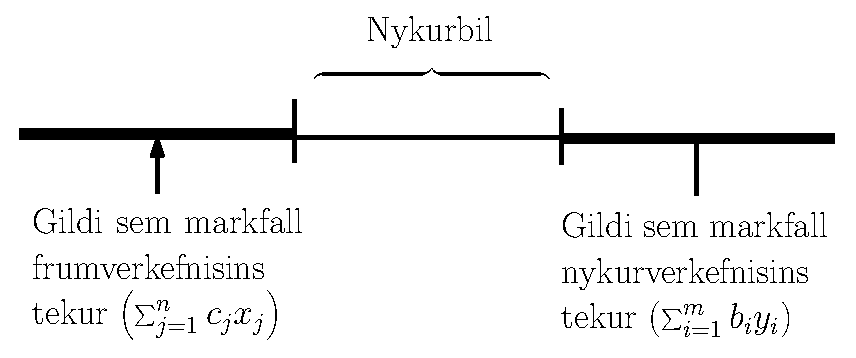
\includegraphics[width=0.6\columnwidth]{figs/nykurbil.eps}
\end{figure}
\begin{setn}[\ath{Sterka nykursetningin} (e. strong duality theorem)] Ef $\vec{x}^*=(x_1^*,...,x_n^*)$ er besta lausn á frumverkefninu. Þá er $\vec{y}^*=(y_1^*,...,y_m^*)$ besta lausn nykurverkefnisins og 
$$\vec{c}^T\vec{x}^*=\vec{b}^T\vec{y}^*$$
 \end{setn}
 Setningin segir að ef til er besta lausn á frumverkefninu þá er ekkert nykurbil. 
Höfum því fjóra möguleika
\begin{enumerate}
 \item Besta lausn til á bæði frum og nykur (ekkert bil)
 \item Frum ótakmarkað, nykur ógjaldgengt (ekkert bil)
 \item Frum ógjaldgengt, nykur ótakmarkað (ekkert bil)
 \item Bæði frum og nykur ógjaldgeng (óendanlegt bil)
\end{enumerate}
\begin{samepage}
\begin{aths}\hspace{.1cm}
 \begin{enumerate}
  \item Efri og neðri mörk á markfalli geta komið að margvíslegum notum, t.d.
 \begin{enumerate}[label=(\roman{*})]
  \item Til að ákvarða hvenær á að stoppa bestunarreiknirit (t.d. innri punkta aðferðir)\\
  $\rightarrow$ stopp þegar $\left|\vec{b}^T\vec{y}-\vec{c}^T\vec{x}\right|\leq \epsilon$, þar sem $\epsilon>0$ er lítil tala.
  \item Takmarka lausnarsvæði í heiltölubestun (sjá kafla \ref{ch:ip}).
 \end{enumerate}
 \item Í endurbættri Simplex-aðferðinni skiptir fjöldi skorða ($m$) meira máli en fjöldi breyta ($n$) fyrir tímann sem útreikningar taka. Þess  vegna getur verið hagkvæmara að leysa nykurverkefnið ef $m\gg n$.
 \end{enumerate}
\end{aths}
\end{samepage}
\begin{samepage}
\begin{daemi}\label{daemi:frum}
Fyrirtækið \emph{Frum} framleiðir tækjabúnað og glingur.
\begin{enumerate}
\item Eitt kíló af tækjabúnaði þarfnast 1 vinnustundar, 1 einingu af timbri, 2 einingar af málmi, og er þá hagnaðurinn 5 evrur.
\item Eitt kíló af glingri  þarfnast 2 vinnustunda, 1 einingu af timbri, 1 einingar af málmi, og hagnaðurinn er þá 4 evrur.
\item Tiltækar vinnustundir eru 120, 70 einingar af timbri og 100 einingar af málmi.
\end{enumerate}
Hversu mikið af tækjabúnaði $x_1$ og glingri $x_2$ á fyrirtækið að framleiða til að hámarka hagnað? 
\end{daemi}
\end{samepage}

\begin{lausn}Línuleg bestunarverkefni fyrir \emph{Frum} er eftirfarandi 
$$ \mbox{Hámarka hagnað:} \quad \max_{x_1,x_2} z = 5 x_1 + 4 x_2  \mbox{ (evrur) }  $$
m.t.t. sk. 
\[ \begin{array}{lrcl}
\mbox{Vinnustundir:} & x_1 + 2 x_2 &\le& 120 \\
\mbox{Timbur:} & x_1 + x_2 &\le &70  \\
\mbox{Málmur:}& 2x_1 + x_2 &\le& 100 \\
& x_1, x_2 &\ge& 0 
\end{array}\]
\end{lausn}

\begin{daemi}\label{daemi:nykur}
Fyrirtækið \emph{Nykur} vill bjóða í hráefnin sem \emph{Frum}
á og er til í að kaupa hvaða magn sem er. Hvaða verð á
\emph{Nykur} að bjóða þannið að \emph{Frum} selji allt hráefnið?

Látum $y_1$, $y_2$, $y_3$ vera verðin fyrir eina
vinnustund, eina einingu af timbri og eina einingu af málmi.
Verðin þurfa að vera nógu há þannig að það borgi sig fyrir
\emph{Frum} að selja frekar en að framleiða tækjabúnað og glingur, þ.e.a.s.
$y_1+y_2+2y_3\ge 5 \mbox{ og } 2y_1+y_2+y_3\ge 4$.

Fyrirtækið \emph{Nykur} vill vitaskuld ekki greiða of mikið,
þannig fáum við nýtt (nykur-)verkefni.
\end{daemi}
\begin{lausn}
$$\textrm{Lágmarka verð:}\quad\min_{y_1,y_2,y_3} w = 120 y_1 + 70 y_2 + 100 y_3  \mbox{ (evrur)}  $$
m.t.t. sk.
\[ \begin{array}{lrclc}
\mbox{Tækjabúnaður:} & y_1 + y_2 + 2y_3 &\ge& 5 & \mbox{ (evrur)}\\
\mbox{Glingur:} & 2y_1 + y_2 + y_3 &\ge& 4 & \mbox{ (evrur)}\\
 & y_1, y_2, y_3 &\ge& 0 
   \end{array}
\]
 \end{lausn}
\begin{samepage}
Skoðum nú sambandið á milli lausna frum- og nykurverkefna.
\begin{lausn}[á dæmum \ref{daemi:frum} og \ref{daemi:nykur}]
Fyrst lítum við á frumverkefnið leyst með Simplex aðferðinni:
{\scriptsize
\[\begin{array}{|c|ccccc|c|}\hline
z & x_1 & x_2 & x_3 & x_4 & x_5 & HH\\ \hline 
     1 & -5 & -4 &  0 &  0 &  0 &  0 \\
     0 &  1 &  2 &  1 &  0 &  0 &  120 \\
     0 &  1 &  1 &  0 &  1 &  0 & 70 \\
     0 &  2 &  1 &  0 &  0 &  1 &  100 \\ \hline 
\multicolumn{7}{l}{>> T=pivot(T,4,2)} \\  \hline 
    1 & 0 &-1.5 & 0 & 0 & 2.5 &  250 \\
    0 & 0 & 1.5 & 1 & 0 &-0.5 &  70 \\
    0 & 0 & 0.5 & 0 & 1 &-0.5 &  20 \\
    0 & 1 & 0.5 & 0 & 0 & 0.5 &  50 \\ \hline 
\multicolumn{7}{l}{>> T=pivot(T,3,3)} \\ \hline 
     1  &   0  &   0  &   0  &   3 &    1 &  310 \\
     0  &   0  &   0  &   1  &  -3 &    1 &   10 \\
     0  &   0  &   1  &   0  &   2 &   -1 &   40 \\
     0  &   1  &   0  &   0  &  -1 &    1 &   30 \\ \hline
  \end{array}\]}
Lesum úr lokatöflunni:
\begin{eqnarray*}
 \vec{x}^* &=&  (30, 40, 10, 0, 0) \\ z^* &=& 310 \\ \vec{y}^* &=& (0, 3, 1)
\end{eqnarray*}
\end{lausn}
\end{samepage}
Leysum nú nykurverkefnið með stóru $M$-aðferðinni í \textsc{matlab}:
\begin{lstlisting}
>> syms M
>> format rational
>> Tdual=[-1 b' zeros(1,n) M M 0; zeros(n,1) A' -eye(n) eye(n) c]
 
Tdual =
 
[ -1, 120, 70, 100,  0,  0, M, M, 0]
[  0,   1,  1,   2, -1,  0, 1, 0, 5]
[  0,   2,  1,   1,  0, -1, 0, 1, 4]
 
>> Tdual = pivot(Tdual,2,7) % Koma grunnbr x6 a eiginlegt form
 
Tdual =
 
[ -1, 120 - M, 70 - M, 100 - 2*M,  M,  0, 0, M, -5*M]
[  0,       1,      1,         2, -1,  0, 1, 0,    5]
[  0,       2,      1,         1,  0, -1, 0, 1,    4]
 
>> Tdual = pivot(Tdual,3,8) % Koma grunnbr x7 a eiginlegt form
 
Tdual =
 
[ -1, 120 - 3*M, 70 - 2*M, 100 - 3*M,  M,  M, 0, 0, -9*M]
[  0,         1,        1,         2, -1,  0, 1, 0,    5]
[  0,         2,        1,         1,  0, -1, 0, 1,    4]
 
>> % Hefjum Simplex-bestun --------------------------------------
>> Tdual = pivot(Tdual,2,4)
 
Tdual =
 
[-1,70-(3*M)/2, 20-M/2, 0, 50-M/2, M, (3*M)/2-50, 0,-(3*M)/2-250]
[ 0,       1/2,    1/2, 1,   -1/2, 0,        1/2, 0,         5/2]
[ 0,       3/2,    1/2, 0,    1/2,-1,       -1/2, 1,         3/2]
 
>> Tdual = pivot(Tdual,3,2)
 
Tdual =
 
[ -1, 0, -10/3, 0, 80/3, 140/3, M - 80/3, M - 140/3, -320]
[  0, 0,   1/3, 1, -2/3,   1/3,      2/3,      -1/3,    2]
[  0, 1,   1/3, 0,  1/3,  -2/3,     -1/3,       2/3,    1]
 
>> Tdual = pivot(Tdual,3,3)
 
Tdual =
 
[ -1, 10, 0, 0, 30, 40, M - 30, M - 40, -310]
[  0, -1, 0, 1, -1,  1,      1,     -1,    1]
[  0,  3, 1, 0,  1, -2,     -1,      2,    3]
 
>> % Bestun lokid; tokum ut gervibreytur
 
Tdual =
 
[ -1, 10, 0, 0, 30, 40, -310]
[  0, -1, 0, 1, -1,  1,    1]
[  0,  3, 1, 0,  1, -2,    3] 
\end{lstlisting}
Lesum úr lokatöflunni:
\begin{eqnarray*}
 \vec{y}^* &=& (0, 3, 1,0,0)\\ z^* &=& 310 \\ \vec{x}^* &=&  (30, 40) 
\end{eqnarray*}

\begin{figure}[t!]
\centering
 \includegraphics[width=0.85\columnwidth]{figs/wyndor_frumlausn.eps}
 \caption{Myndræn lausn á frumverkefninu \ref{daemi:frum}} 
 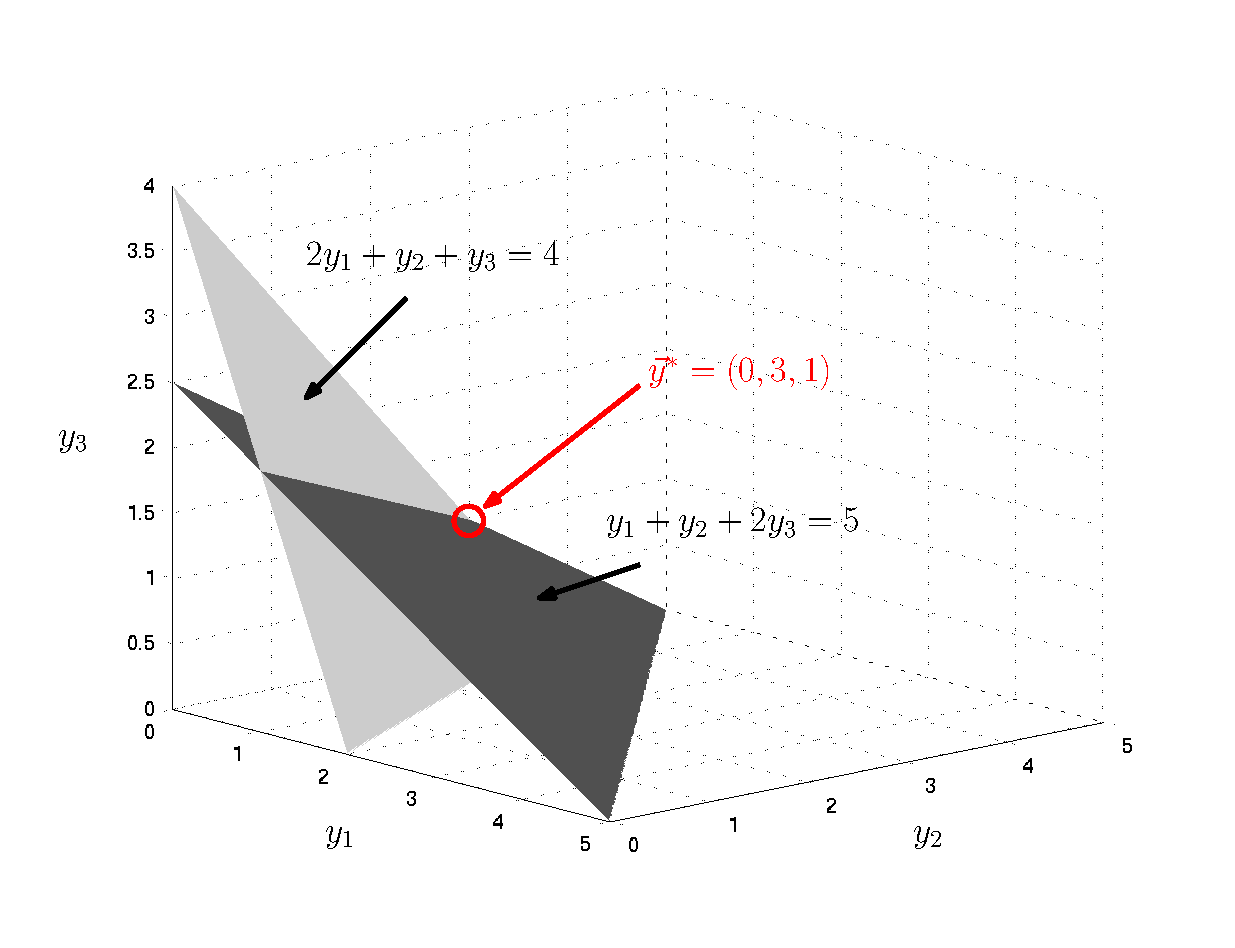
\includegraphics[width=0.85\columnwidth]{figs/wyndor_nykurlausn.eps}
 \caption{Myndræn lausn á nykurverkefninu \ref{daemi:nykur}} 
\end{figure}
%\end{lausn}

\begin{samepage}
\section{Hagfræðileg túlkun nykurverkefna}
Um frumverkefnið gildir
\begin{itemize}
 \item[$x_j$] Magn sem framleitt er af vöru (e. activity) $j$, $j\in\{1,...,n\}$.
 \item[$c_j$] Framlegð af vöru $j$ (á einingu).
 \item[$z$] Heildarhagnaður.
 \item[$b_i$] Magn af hráefni (e. resource) $i$ sem er til ráðstöfunar, $i\in\{1,...,m\}$.
 \item[$a_{ij}$] Magn af hráefni $i$ sem þarf til þess að framleiða eina einingu af vöru $j$.
\end{itemize}
Í sérhverri ítrun er gildi markfallsins
$$w=\sum_{i=1}^m b_iy_i$$
þ.e. framlag $b_i$ eininga af hráefni til markfallsins er $y_ib_i$ og því má túlka $y_i$ sem framlag einnar einingar af hráefni $i$ til markfallsins. Gildin á $y_i$ ($y_i^*$ í bestu lausn) kallast \ath{skuggaverð} (e. shadow price), $y_i^*=\frac{\partial w^*}{\partial b_i}$.

Við framleiðslu á vöru $j$ eru notaðar $a_{ij}$ einingar af hráefni $i$ og $\sum_{i=1}^m a_{ij}y_i$ er því framlag til markfalls af \emph{hráefnisblöndunni} sem þarf til að framleiða eina einingu af vöru $j$. Þessa hráefnisblöndu mætti einnig nota við framleiðslu á öðrum vörum. Það er einungis skynsamlegt ef $\sum_{i=1}^m a_{ij}y_i\geq c_j$ (annars værum við ekki að nota hráefnin á hagkvæmasta máta).
\end{samepage}
\section{Tengsl frum- og nykurverkefna}
%\footnotetext{skoðið líka töflurnar í kafla 6.4 H\&L}
\begin{description}
 \item[\ath{Frumverkefni} $P$] (e. primal):
\begin{eqnarray*}
\max & z = \sum_{j=1}^n c_j x_j & \\
\mbox{sk.} & \sum_{j=1}^n a_{ij}x_j \le b_i, & i \in \mathcal{I}_1\\
 & \sum_{j=1}^n a_{ij}x_j \ge b_i, & i \in \mathcal{I}_2\\
 & \sum_{j=1}^n a_{ij}x_j = b_i, & i \in \mathcal{I}_3 \\
 & x_j \ge 0, & j \in \mathcal{J}_1  \\
 & x_j \le 0, & j \in \mathcal{J}_2  \\
 & x_j \ ^>_<\  0, & j \in \mathcal{J}_3  
\end{eqnarray*}
 \item[\ath{Nykurverkefni} $D$] (e. dual):
\begin{eqnarray*}
\min & w = \sum_{i=1}^m b_i y_i & \\
\mbox{sk.} & \sum_{i=1}^m a_{ij}y_i \ge c_j, & j \in \mathcal{J}_1\\
 & \sum_{i=1}^m a_{ij}y_i \le c_j, & j \in \mathcal{J}_2\\
 & \sum_{i=1}^m a_{ij}y_i = c_j, & j \in \mathcal{J}_3 \\
 & y_i \ge 0, & i\in \mathcal{I}_1  \\
 & y_i \le 0, & i\in \mathcal{I}_2  \\
 & y_i \ ^>_<\  0, & i \in \mathcal{I}_3  
\end{eqnarray*}
\end{description}

\begin{aths}Um gagnvirk verkefni gildir:
\begin{itemize}
\item Til sérhverra skorðu í ($P$) svarar nykurbreyta.
\item Til sérhverra skorðu í ($D$) svarar frumbreyta.
\item Stuðlar markfalls ($P$) eru hægri hlið (HH) í ($D$)
\item Stuðlar markfalls ($D$) eru HH í ($P$)
\item Gagnvirkt (nykur) verkefni gagnvirka verkefnisins er upphaflega (frum) verkefnið, þ.e. nykur af nykur er frum. 

\begin{lausn}
{\scriptsize
\begin{eqnarray*}
\begin{array}{lc} \max & \vec{c}^T\vec{x}\\ \textrm{sk.}&\vec{A}\vec{x}\leq \vec{b} \\ & \vec{x}\geq\vec{0}\end{array}
&\stackrel{\textrm{nykur}}{\rightarrow}&
\begin{array}{lc} \min & \vec{b}^T\vec{y}\\ \textrm{sk.}&\vec{y}^T\vec{A}\geq \vec{c} \\ & \vec{y}\geq\vec{0}\end{array} 
\stackrel{\textrm{staðlað form}}{\rightarrow}
\begin{array}{lc} \max & -\vec{b}^T\vec{y}\\ \textrm{sk.}&-\vec{y}^T\vec{A}\leq -\vec{c} \\ & \vec{y}\geq\vec{0}\end{array} 
\\&\stackrel{\textrm{nykur}}{\rightarrow}&
\begin{array}{lc} \min & -\vec{c}^T\vec{x}\\ \textrm{sk.}&-\vec{A}\vec{x}\geq -\vec{b} \\ & \vec{x}\geq\vec{0}\end{array} 
\stackrel{\textrm{staðlað form}}{\rightarrow}
\begin{array}{lc} \max & \vec{c}^T\vec{x}\\ \textrm{sk.}&\vec{A}\vec{x}\leq \vec{b} \\ & \vec{x}\geq\vec{0}\end{array}  
\end{eqnarray*}}\end{lausn}
Það skiptir því ekki máli hvort verkefnið við köllum frum eða nykur. Venjan er þó að kalla verkefnið sem við setjum (fyrst) fram, frumverkefni. 
\item Stundum er mun ódýrara að leysa gagnvirk (nykur) verkefni en það upphaflega (frum). Það gildir þegar skorður eru mun fleiri en fjöldi breyta, $m \gg n$.
\item $w^* = \vec{y}^*\vec{b}  = \vec{c}^T \vec{x}^* = z^*$ (notum $^*$ til að tákna bestu lausn, sjá líka bls. 201 í H\&L, e. strong duality property).
\item Ef $\vec{x}$ er gjaldgeng lausn í frumverkefninu og $\vec{y}$ er leyfileg lausn í nykur\-verkefninu þá er $\vec{c}^T\vec{x}\le \vec{y}\vec{b}$ (e. weak duality property).
\item Í hverri ítrun simplex aðferðarinnar þá er fundin leyfileg grunnlausn (BFS) $\vec{x}$ og samsvarandi $\vec{y}$ fyrir nykurverkefnið, $\vec{c}\vec{x}=\vec{y}\vec{b}$ (e. complementary solution property). Ef $\vec{x}$ er ekki besta lausn í ($P$) þá er $\vec{y}$ ekki gjaldgeng lausn í ($D$).
\end{itemize}
\end{aths}


Rifjum upp Simplex-töfluna á fylkjaformi (fyrir hvaða ítrun sem er):
\begin{center}
{\renewcommand{\arraystretch}{1.5} \renewcommand{\tabcolsep}{0.2cm}{\footnotesize
\[ \begin{array}{|cc|c|cc|c|}\hline 
  \textrm{Grunnbr.} & \textrm{Jafna} & z & \textrm{Upphafl. br.} & \textrm{Slakabr.} & \textrm{Hægri hlið} \\ \hline\hline
  z & (0) & 1 & \vec{c}_B\vec{B}^{-1}\vec{A}-\vec{c} & \vec{c}_B\vec{B}^{-1} & \vec{c}_B\vec{B}^{-1}\vec{b} \\
\vec{x}_B & (1,\ldots,m) & \vec{0} & \vec{B}^{-1}\vec{A} & \vec{B}^{-1} & \vec{B}^{-1}\vec{b} \\ \hline
 \end{array}\]}}\end{center}
Athugum nánar jöfnu $(0)$. Látum $z=\vec{c}_B^T\vec{B}^{-1}\vec{A}=\vec{y}\vec{A}$, þá er $z_j=\sum_{i=1}^m y_i a_{ij}$ og jafna $(0)$ verður
\[ \begin{array}{cccccc|c}
 x_1 & \cdots & x_n & x_{n+1} & \cdots & x_{n+m} & HH \\
 z_1-c_1 & \cdots & z_n-c_n & y_1 & \cdots & y_m & w=\vec{y}^T\vec{b}    
\end{array}\]
Skorða $j$ í nykurverkefninu er $z_j=\sum_{i=1}^m a_{ij}y_i\geq c_j$ (sbr. $\vec{y}^T\vec{A}\geq\vec{c}$) og því má túlka $z_j-c_j$ sem \ath{umframbreytu} (e. surplus variable) fyrir skorðuna (er 0 þegar skorðan er \emph{bindandi}).

Í frumverkefninu fæst grunnlausn m.þ.a. skeyta slakabreytum við $x$-in. Hliðstætt því fæst grunnlausn í nykurverkefni m.þ.a. skeyta umframbreytum við $y$-in, þ.e. $$ (y_1,...,y_m,z_1-c_1,...,z_n-c_n).$$ Nykurverkefni á viðskeyttu formi hefur $n$ breytur í grunni og $m$ utan grunns.

\begin{samepage}
Eftirfarandi samband gildir milli $P$ og $D$
\begin{center}
 \begin{tabular}{lll}
  Frumbreyta 		&	Tilsvarandi nykurbreyta \\ \hline 
  Ákv.br. $x_j$		&	Slakabr. $z_j-c_j$	& $j\in\{1,...,n\}$ \\
  Slakabr. $x_{n+i}$	&	Ákv.br. $y_i$		& $i\in\{1,...,m\}$
 \end{tabular}
\end{center}
Í sérhverri ítrun finnur Simplex-aðferðin gjaldgenga hornpunktslausn $P$ og einnig svonefnda \ath{fyllingalausn} (e. complementary solution) fyrir $D$ þar sem $\vec{c}^T\vec{x}=\vec{b}^T\vec{y}$ (ef $\vec{x}$ er ekki besta lausnin á $P$ þá er $\vec{y}$ ekki gjaldgeng í $D$).
\end{samepage}

\begin{figure}[t!]
\centering
\includegraphics[width=0.7\columnwidth]{figs/complementary.eps}
\end{figure}

Tilsvarandi gildir um grunnlausnir $P$ og $D$. Svarandi til sérhverrar grunn\-lausnar $P$ er \ath{fyllingagrunnlausn} (e. complimentary basic solution) á $D$ og markfallsgildi þeirra ($z$ og $w$) eru þau sömu. Auk þess gildir:
\begin{center}
 \begin{tabular}{ll}
  Frumbreyta 		&	Tilsvarandi nykurbreyta \\ \hline 
  Í grunni $(>0)$	&	Utan grunns $(=0)$	\\
  Utan grunns $(=0)$	&	Í grunni $(>0)$		
 \end{tabular}
\end{center}

Þegar önnur lausnin (frum eða nykur) er þekkt má finna hina með því að leysa jöfnuhneppi.

\begin{setn}[\ath{Complimentary slackness}] Ef $(x_1,...,x_n)$ er besta lausn á $P$ og $(y_1,...,y_m)$ er besta lausn á $D$ þá gildir:
\begin{enumerate}
 \item $x_j(z_j-c_j)=0$ \quad\quad ($z_j-c_j$ er umframbr. í $D$)
 \item $x_{n+1}y_i=0$\quad\quad\quad~~~($x_{n+1}$ er slakabr. í $P$)
\end{enumerate}
fyrir öll $i$ og $j$.
\end{setn}
\begin{proof}Sjáum að strax að 1. og 2. eru tilsvarandi tilvik. 
Höfum að 
\begin{eqnarray*}
\sum_{j=1}^n c_jx_j &\stackrel{(\star)}{\leq}& \sum_{j=1}^n\left(\sum_{i=1}^m a_{ij}y_i\right)x_j
\end{eqnarray*}
því $c_j\leq\sum_{i=1}^m a_{ij}y_i$ (sjá veiku nykursetninguna \ref{setn:veiknykur}).
Jafnaðarmerkið í $(\star)$ gildir annaðhvort þegar
\begin{enumerate}[label=(\roman{*})]
 \item $x_j=0$ fyrir öll $j\in\{1,...,n\}$,
 \item eða $c_j=\sum_{i=1}^m a_{ij}y_i=z_j$ þ.e. $z_j-c_j=0$.
\end{enumerate}
\end{proof}

\section{Frumverkefni sem eru ekki á stöðluðu formi}
Getum alltaf komið línulegu bestunarverkefni yfir á staðlað form 
{\renewcommand{\arraystretch}{1.5} \renewcommand{\tabcolsep}{0.2cm}
\begin{eqnarray*}
 \min z &\rightarrow& \max -z \\
 \vec{a}^T\vec{x}\geq \vec{b} &\rightarrow& -\vec{a}^T\vec{x}\leq-\vec{b} \\
 \vec{a}^T\vec{x}= \vec{b} &\rightarrow& \vec{a}^T\vec{x}\geq \vec{b} \textrm{ og } \vec{a}^T\vec{x}\leq \vec{b} \\
 x_i \textrm{ frjáls } &\rightarrow& x_i=x_i^+-x_i^- \textrm{ með } x_i^+,x_i^-\geq 0.
\end{eqnarray*}}
\begin{aths}
Á bls. 213--215 í H\&L eru nokkur trix sem stytta manni leið við að ákvarða form skorða og breyta í nykurverkefnum. 
\end{aths}
\begin{center}{\renewcommand{\arraystretch}{1.5} \renewcommand{\tabcolsep}{0.2cm}
\begin{tabular}{|ccc|}\hline 
Annað verkefnið && Hitt verkefnið \\ \hline 
$\max z$ (eða $w$) && $\min w$ (eða $z$) \\ \hline
skorða $i$ && breyta $y_i$ (eða $x_i$) \\
$\leq$ &$\longleftrightarrow$& $y_i\geq0$ \\ 
$=$ &$\longleftrightarrow$ & $y_i$ óskorðað \\
$\geq$ &$\longleftrightarrow$& $y_i\leq0$ \\ \hline 
breyta $x_j$ (eða $y_j$) && skorða $j$ \\  
$x_j\geq0$ &$\longleftrightarrow$ & $\geq$ \\ 
$x_j$ óskorðað &$\longleftrightarrow$ & $=$ \\
$x_j\leq0$ &$\longleftrightarrow$& $\leq$ \\ \hline 
\end{tabular}}
\end{center}

\begin{daemi}[Nykurverkefni geisladæmisins \ref{daemi:krabbi}]Höfum frumverkefni:
\begin{center}{\renewcommand{\arraystretch}{1.5} \renewcommand{\tabcolsep}{0.2cm}
\begin{tabular}{|l|rrr|}\hline
Heildarmagn geislunar & \multicolumn{3}{c|}{$\max_{x_1,x_2} -z = -0.4x_1 - 0.5x_2$} \\ \hline
Heilbrigðir vefir & $0.3x_1$ & $+\; 0.1x_2$ & $ \le  2.7 $ \\
Krabbameinssvæði & $ 0.5x_1 $&$ +\; 0.5x_2 $&$=  6.0 $ \\
Miðja æxlis & $0.6x_1$&$ +\; 0.4x_2$& $\ge 6.0$ \\ 
& \multicolumn{3}{c|}{$x_1,x_2 \ge 0$} \\ \hline
\end{tabular}} 
\end{center}
\end{daemi}
\begin{lausn}Þá er nykurverkefnið:
\begin{center}{\renewcommand{\arraystretch}{1.5} \renewcommand{\tabcolsep}{0.2cm}
\begin{tabular}{|l|rrrr|}\hline
&\multicolumn{4}{c|}{$\min_{y_1,y_2,y_3} w = 2.7y_1 + 6y_2+6y_3$} \\ \hline
Geisli 1: & $0.3y_1$ & $+\; 0.5y_2$& $+\; 0.6y_3$ & $ \ge -0.4 $ \\
Geisli 2: & $0.1y_1 $&$ +\; 0.5y_2$& $+\; 0.4y_3$& $ \ge -0.5 $ \\
& \multicolumn{4}{c|}{$y_1 \ge 0$} \\ 
& \multicolumn{4}{c|}{$y_2$ óskorðað}  \\ 
& \multicolumn{4}{c|}{$y_3 \le 0$} \\ \hline
\end{tabular}} 
\end{center} 
\end{lausn}
\section{Strangt fyllingarskilyrði}
Um \ath{ströng fyllingarskilyrði} (e. strict complement\-arity) höfum við: 
\begin{itemize} 
\item Ef strangt fyllingarskilyrði \emph{gildir}, en það segir að allar grunnbreytur séu $\ne 0$ (breytur utan grunns eru jú $0$, en þetta þýðir að engar aðrar breytur séu $0$ \emph{fyrir tilviljun}). Þá gildir: 
  \begin{enumerate}[label=(\roman{*})]
  \item\label{fylli1} $x$ er grunnbreyta þ.þ.a.a. tilsvarandi nykur skorða er virk, þ.e.a.s.
  \begin{eqnarray*}
      x_j\ne 0 & \Longleftrightarrow &\vec{a}_j^T\vec{y} = c_j \\
      x_i^{\mbox{\tiny slaka}} \ne 0 \mbox{  (þ.e. $\vec{a}_i\vec{x}\ne b_i$)} & \Longleftrightarrow & y_i = 0 
   \end{eqnarray*}
   \item\label{fylli2} Ef upphafleg (frum) skorða er virk þ.þ.a.a. tilsvarandi nykur \mbox{breyta} er í grunni, þ.e.a.s. 
  \begin{eqnarray*}
  \vec{a}_i\vec{x} = b_i &\Longleftrightarrow & y_i \ne 0 \\
  x_j = 0  & \Longleftrightarrow & y_j^{\mbox{\tiny slaka}} \ne 0 \mbox{  (þ.e. $\vec{a}_j^T\vec{y}\ne   c_j$)}
  \end{eqnarray*}
  \end{enumerate}
  \begin{aths}Ljóst er að \ref{fylli1} er jafngilt \ref{fylli2}.\end{aths}
  \item Ef strangt fyllingarskilyrði \emph{gildir ekki}, hefur í för með sér að til eru lausnir á frumverkefni og því gagnvirka (nykur):
  \begin{eqnarray*}
  x_j \textrm{ er í grunni } & \Longleftrightarrow & y_j^{\textrm{\textrm{\tiny slaka}}} \textrm{ er utan grunns} \\
  x_i^{\mbox{\tiny slaka}}\textrm{ er í grunni } &\Longleftrightarrow& y_i \textrm{ er utan grunns}  
  \end{eqnarray*}
\begin{aths}Þó skorðan $\vec{a}_j^T\vec{y} = c_j$ sé virk er ekki nauðsynlegt að tilsvarandi slakabreyta sé utan grunns.\end{aths}
\end{itemize}

\section{Næmnigreining og nykurverkefni}\label{sec:naemnigreining}
\ath{Næmnigreining} (e. sensitivity analysis) kannar áhrif breytinga á $c_j, b_i$ og $a_{ij}$ á bestu lausn.
\begin{itemize}
 \item Er lausnin gjaldgeng eftir breytingu?
 \item Er hún enn best?
\end{itemize}
Þessum spurningum (ásamt fleiri) má oft svara með lítilli fyrirhöfn m.þ.a. nýta vensl milli frum- og  nykurverkefna. Sjaldnast þarf að leysa líkanið frá grunni.

\begin{daemi}[Ný vara bætist við hjá Wyndor úr dæmi \ref{wyndor:org}]\label{wyndor:new}
$$\max_{\vec{x}} z= 3x_1+5x_2+4x_{\textrm{ný}} $$
m.t.t. skorðanna
\[\begin{array}{ccccccc}
 x_1 &   &      &+& 2x_{\textrm{ný}} & \leq & 4 \\
     &   & 2x_2 &+& 3x_{\textrm{ný}} & \leq &12 \\
 3x_1& + & 2x_2 &+&  x_{\textrm{ný}} & \leq &18\\
\multicolumn{7}{c}{x_1,x_2,x_{\textrm{ný}}\geq0}
\end{array}\]
Besta lausn sem við fundum fyrir upphaflega verkefnið var \mbox{$x_1=2$},\mbox{$x_2=6$} og því $x_{\textrm{ný}}=0$. Hún er augljóslega gjaldgeng, en er hún enn best?
\end{daemi}
\begin{lausn}Ný breyta í frumverkefni svarar til nýrrar skorðu í nykurverkefni:
\begin{equation}\label{sk:13}
 2y_1+3y_2+y_3\geq4 
\end{equation}
Lesum fyllingalausnina $(\vec{y}^*,\vec{z}^*-\vec{c}^*)=(y_1^*,y_2^*,y_3^*,z_1^*-c_1^*,z_2^*-c_2^*)$ beint út úr loka Simplex-töflunni (sjá lausn á bls. \pageref{wyndor:simplex}):
\begin{center}
{\renewcommand{\arraystretch}{1.5} \renewcommand{\tabcolsep}{0.2cm}
{\scriptsize
$\begin{array}{|c|ccccc|c|} \hline 
\textrm{grunnbr.} &  x_1 &  x_2 &   x_3 &  x_4 &  x_5 &  HH  \\ \hline 
z   &0 & 0 & 0 & \frac{3}{2} & 1 &  36 \\
x_3& 0 & 0 & 1 & \frac{1}{3} & -\frac{1}{3} & 2 \\
x_2& 0 & 1 & 0 & \frac{1}{2} & 0 & 6  \\
x_1& 1 & 0 & 0 &-\frac{1}{3} & \frac{1}{3} & 2  \\ \hline 
\end{array}$
}}\end{center}
þ.e. skorða \eqref{sk:13} fyrir $\vec{y}^*$ verður
$$2\cdot 0+3\cdot \frac{3}{2}+1\cdot1=\frac{11}{2} =5.5\geq 4.$$
Nykurlausnin er gjaldgeng, frumlausnin er gjaldgeng og lausnin er því ennþá best.
\begin{samepage}
\begin{aths}\hspace{.1cm}
  \begin{enumerate}[label=(\roman{*})]
  \item Framlegð $c_{\textrm{ný}}$ er ekki nógu mikil til þess að Wyndor hafi ávinning á því að framleiða þessa nýju vöru.
  \item Önnur leið að sömu niðurstöðu væri að leysa líkanið upp á nýtt.
  \end{enumerate}
\end{aths}\end{samepage}
\end{lausn}

Næmnigreining er mikilvæg í línulegri bestun því gert er ráð fyrri að stikar líkansins ($b_i,c_j,a_{ij}$) eru \emph{þekktir fastar}. Oft eru gildi á stikunum  einhvers konar spá um ástönd sem gilda í framtíðinni (t.d. framlegðartölur) og stikamatið því háð talsverðri óvissu. Í öðrum tilvikum geta gildi á stikunum endurspeglað ákvarðanir sem e.t.v. eru ekki vel ígrundaðar eða væri auðvelt að breyta. Dæmi um slíkt gæti verið tími til umráðana hjá Wyndor.
% Undantekning: Kerfislíffræði
Þess vegna er mikilvægt að kanna hvernig líkanið bregst við breytinum á stikum. Finna þarf hvaða stikar hafa mikil áhrif (e.t.v. þarf að endurmeta einhverja þeirra í framhaldinu). Fyrir þá stika sem hafa tiltölulega lítil áhrif á er gagnlegt að vita á hvaða bili þeir mega liggja án þess að besta lausn breytist að ráði. 

\section{Framgangsmáti næmnigreiningar}
\begin{enumerate}
 \item Uppfæra líkan m.t.t. breytinga á stikum.
 \item Uppfæra loka Simplex-töfluna.
 \item Koma töflunni yfir á eiginlegt form með Gauss-eyðingu.
 \item Er lausnin gjaldgeng? (þ.e. hægri hlið $\geq0$)
\end{enumerate}
\begin{tabular}{llp{10cm}}
\hspace{1cm} & Nei $\rightarrow$ & Besta aftur (laga lokatöflu og nota sem upphafs\-töflu).\\
& Já  $\rightarrow$ & Er lausnin ennþá best? (allir stuðlar í línu $(0)$ eru $\geq 0$)\\
& & Nei $\rightarrow$\quad Ítra með Simplex-aðferðinni.
\end{tabular}

\begin{aths}Ekki er alltaf nauðsynlegt að framkvæma öll þessi skref.\end{aths}

Þessi framgangsmáti miðar við að við viljum framkvæma næmnigreiningu á reikningslega hagkvæman máta, þ.e. ekki leysa líkönin ítrekað frá grunni, fyrir mismunandi gildum á stikunum t.d. $b_1=1,b_1=1.1,b_1=1.2$ o.s.frv.

Við finnum hvernig lokataflan myndi líta út ef við byrjum með nýju gildin $(\overline{\vec{c}},\overline{\vec{b}},\overline{\vec{A}})$ í upphafstöflunni, beitum sömu grunnaðgerðum (Gauss-eyðing) og við gerðum við með upphaflegu gildunum. 
%\begin{aths}Við fengjum líklegast aðra lokatöflu ef við beitum Simplex á $\vec{c},\vec{A}$ og $\vec{b}$.\end{aths}


\begin{table}[h!]
\begin{center}
{\renewcommand{\arraystretch}{1.5} \renewcommand{\tabcolsep}{0.2cm}
\begin{tabular}{|ll|}\hline 
$\overline{\vec{A}}$ & $\vec{A}$ fylki eftir breytingu,\\
$\overline{\vec{b}}$ & hægri hlið eftir breytingu,\\
$\overline{\vec{c}}$ & markfallsstuðlar eftir breytingu,\\
$\vec{y}^*$ & skuggaverð í lokatöflu,\\
$\vec{S}^*$ & stuðlar við slakabreytur í lokatöflu.\\\hline
\end{tabular}}
\caption{Ritháttur}
\end{center}
\end{table}

\begin{samepage}\begin{aths}Algengara er að skoða áhrif þess að breyta einum stika í einu heldur en mörgum í einu.\end{aths}\end{samepage}

\begin{samepage}
Lokatafla eftir breytingar
\begin{center}
{\renewcommand{\arraystretch}{1.5} \renewcommand{\tabcolsep}{0.2cm}
{\footnotesize
\[ \begin{array}{|c|c|cc|c|}\hline 
 \textrm{Jafna} & z & \textrm{Ákv.br.} & \textrm{Slakabr.} & \textrm{Hægri hlið} \\ 
& & x_1,...,x_n & x_{n+1},...,x_{n+m} & \\ \hline
(0) & 1 & \vec{y}^*\overline{\vec{A}}-\overline{\vec{c}} & \vec{y}^* & \vec{y}^*\overline{\vec{b}}=z^* \\
(1,\ldots,m) & \vec{0} & \vec{S}^*\overline{\vec{A}} & \vec{S}^{*} & \vec{S}^{*}\overline{\vec{b}} \\ \hline
 \end{array}\]
}}
\end{center}
\end{samepage}
\subsection{Breytingar á hægri  hlið}
Þegar breytingar eru gerðar á hægri hlið (þ.e. $\vec{b}$) þá er taflan á réttu formi (Gauss-eyðing óþörf), og svo fremi sem hægri hlið er $\geq0$ (gjaldgeng lausn) eftir breytingarnar er lausnin enn best. Hægri hlið verður (eftir breytingu)
 \begin{eqnarray*}
 \textrm{Jafna }(0) \;:& z^*=\vec{y}^*\overline{\vec{b}} \\
 \textrm{Jafna }(1,...,m)\;: & \vec{b}^*=\vec{S}^*\overline{\vec{b}} \\
 \end{eqnarray*}
 \begin{daemi}[Wyndor úr dæmi \ref{wyndor:org}]\label{wyndor:naemni1} Wyndor fer með $b_2$ úr 12 í 24, þ.e. $$\overline{\vec{b}}=\begin{bmatrix}4\\24\\18\end{bmatrix}.$$ Er upphaflega lausnin enn best?
 \end{daemi}
 \begin{lausn}Lokataflan fyrir upphaflega líkanið (sjá lausn á bls. \pageref{wyndor:simplex})
 \begin{center}
{\renewcommand{\arraystretch}{1.5} \renewcommand{\tabcolsep}{0.2cm}
{\scriptsize
$\begin{array}{|c|cc|ccc|c|} \hline 
 Z &  x_1 &  x_2 &   x_3 &  x_4 &  x_5 &  HH   \\ 
\hline\hline 
 1 & 0 & 0 & 0 & \frac{3}{2} & 1 &  36 \\ \hline
 0 & 0 & 0 & 1 & \frac{1}{3} & -\frac{1}{3} & 2 \\
 0 & 0 & 1 & 0 & \frac{1}{2} & 0 & 6  \\
 0 & 1 & 0 & 0 &  -\frac{1}{3} & \frac{1}{3} & 2  \\ \hline 
\end{array}$
}}\end{center} 
Þá verður
\begin{eqnarray*}
 z^*&=&\vec{y}\overline{\vec{b}}=\begin{bmatrix}0 &\frac{3}{2}&1\end{bmatrix}\begin{bmatrix}4\\24\\18\end{bmatrix}=36+18=54\\
 \vec{b}^*&=&\vec{S}^*\overline{\vec{b}}=\begin{bmatrix} 1 & \frac{1}{3} & -\frac{1}{3} \\ 0 & \frac{1}{2} & 0\\ 0 & -\frac{1}{3} & \frac{1}{3}\end{bmatrix}\begin{bmatrix}4\\24\\18\end{bmatrix}=\begin{bmatrix}4+8-6\\12\\-8+6\end{bmatrix}=\begin{bmatrix}6\\12\\-2\end{bmatrix}
\end{eqnarray*}
Lausnin (sem áður var best) er því 
$$ (x_1=-2,x_2=12,x_3=6,x_4=x_5=0)\quad\mbox{með}\quad z=36$$
sem er \emph{ekki gjaldgeng} því $x_1=-2<0$. 

\begin{samepage}
Þurfum því að besta aftur (e. reoptimisation) annaðhvort með
\begin{itemize}
 \item Nykur-Simplex aðferðin (7. kafli), eða 
 \item Frá grunni með $\vec{b}=\begin{bmatrix}4\\24\\18\end{bmatrix}$, 
 \begin{center}
{\renewcommand{\arraystretch}{1.5} \renewcommand{\tabcolsep}{0.2cm}
{\scriptsize
\[\begin{array}{|c|cc|ccc|c|} \hline 
 Z &  x_1 &  x_2 & x_3 & x_4 & x_5 &  HH  \\ \hline\hline 
 1 &  -3 &  -5 &  0 &  0 &  0&  0 \\ 
 0 & 1 &  0 &  1 & 0 & 0 &  4 \\
 0 &  0 &  2 &  0 &   1 &   0 & 24 \\
 0 &  3 &  2 & 0 & 0 & 1 &  18 \\ 
\hline\hline \multicolumn{7}{l}{>> T = pivot(T,4,3)} \\ \hline 
 1 &  \frac{9}{2} & 0 & 0 & 0 & \frac{5}{2}& 45 \\ 
 0 &    1 & 0 & 1 & 0 & 0   & 4 \\ 
 0 &   -3 & 0 & 0 & 1 &-1   & 6 \\ 
 0 &  \frac{3}{2} & 1 & 0 & 0 & \frac{1}{2} & 9 \\ \hline 
\end{array}\]
}}\end{center} \end{itemize}\end{samepage}
Nýja besta lausnin er: $$(x_1=0,x_2=9,x_3=4,x_4=6,x_5=0) \quad\mbox{með}\quad z^*=45.$$ Sjáum að við hættum að framleiða vöru 1.
\end{lausn}
Athugum nú á \emph{hvaða bili} (e. allowable range) $\overline{\vec{b}}$ getur legið þ.a. lausnin verði áfram gjaldgeng
$$\vec{b}^*=\vec{S}^*\overline{\vec{b}}=\vec{S}^*(\vec{b}+\Delta\vec{b})=\vec{S}^*\vec{b}+\vec{S}^*\Delta\vec{b}\geq0$$
\begin{daemi}[Leyfileg breyting á hægri hlið Wyndors]\label{wyndor:naemni2} Sáum í dæmi \ref{wyndor:naemni1} að með $b_2=12\rightarrow24=\overline{b}_2$ varð lausnin óleyfileg. Finnum leyfilega breytingu á $b_2$ þ.a. lausnin verði enn gjaldgeng. 
\end{daemi}
\begin{lausn}Höfum $$\vec{S}^*\Delta\vec{b}=\begin{bmatrix}1 &\frac{1}{3}&-\frac{1}{3}\\0 &\frac{1}{2} & 0\\0&-\frac{1}{3}&\frac{1}{3}\end{bmatrix}\begin{bmatrix}0\\\Delta b_2\\0\end{bmatrix}=\begin{bmatrix}\frac{1}{3}\Delta b_2\\\frac{1}{2}\Delta b_2\\-\frac{1}{3}\Delta b_2\end{bmatrix}$$
Þá þarf að gilda
\[\begin{array}{cccl}
2+\frac{1}{3}\Delta b_2 &\geq 0 & \rightarrow &\Delta b_2\geq-6 \\
6+\frac{1}{2}\Delta b_2 &\geq 0 & \rightarrow &\Delta b_2\geq-12 \\
2-\frac{1}{3}\Delta b_2 &\geq 0 & \rightarrow &\Delta b_2\leq6 
\end{array}\]
Því er $\vec{x}^*$ gjaldgengt ef $-6\leq\Delta b_2\leq 6$, eða $12-6\leq b_2\leq 12+6$, þ.e. $6\leq b_2\leq 18$.
\end{lausn}
\subsection{Breyting á stuðlum ákvarðanabreytu ekki í grunni}\label{breyting:nonbasic}
Breyting á stuðlum við $x_j$, þar sem $x_j$ er ekki í grunni þýðir annaðhvort
$$ a_{ij}\rightarrow \overline{a}_{ij}\quad\mbox{og/eða}\quad c_j\rightarrow\overline{c}_j$$
Lausnin verður áfram gjaldgeng í frumverkefni (því $x_j=0$). Ef hún er líka gjaldgeng í nykurverkefni þá er hún enn best.
\begin{daemi}[Afbrigði af Wyndor]\label{daemi:wyndor:afbrigdi}$$\max_{\vec{x}} z=3x_1+5x_2$$ m.t.t. sk. \[\begin{array}{crl} x_1 & &\leq 4\\&2x_2&\leq24\\3x_1&+2x_2&\leq18\end{array}\]
Besta lausnin var fundin í dæmi \ref{wyndor:naemni2} og var $x_1=0,\;x_2=9$ með $z=45$.
Hvernig breytist lausnin þegar $c_1$ og $a_{i1}$ breytist \emph{samtímis} ef 
$$ c_1=3\rightarrow \overline{c}_1=4\quad\mbox{og}\quad \vec{A}_1=\begin{bmatrix}1\\0\\3\end{bmatrix}\rightarrow\overline{\vec{A}}_1=\begin{bmatrix}1\\0\\2\end{bmatrix}$$
\end{daemi}

\begin{lausn}Lokataflan var fundin hér á undan og var 
  \begin{center}
{\renewcommand{\arraystretch}{1.5} \renewcommand{\tabcolsep}{0.2cm}
{\scriptsize
\[\begin{array}{|c|cc|ccc|c|} \hline 
 Z &  x_1 &  x_2 & x_3 & x_4 & x_5 &  HH  \\ \hline
 1 & \frac{9}{2} & 0 & 0 & 0 & \frac{5}{2}& 45 \\ \hline
 0 &    1 & 0 & 1 & 0 & 0   & 4 \\ 
 0 &   -3 & 0 & 0 & 1 &-1   & 6 \\ 
 0 &  \frac{3}{2} & 1 & 0 & 0 & \frac{1}{2} & 9 \\ \hline 
\end{array}\]
}}\end{center} 
Lesum úr töflunni $y_1^*=0,\;y_2^*=0,\;y_3^*=\frac{5}{2}$ með $z^*=45$.

Ein skorða nykurverkefnisins breytist:
\[\begin{array}{llrcc}
 \mbox{Áður:} & y_1+3y_3 &\geq 3 \\
 \mbox{Eftir:} & y_1+2y_3 &\geq 4  &\stackrel{{\scriptstyle \mbox{set inn } \vec{y}^*}}{\Longrightarrow}& 0+2\frac{5}{2}\geq 4,
\end{array}\]
Lausnin er gjaldgeng í nykurverkefninu, og því enn best.
\end{lausn}

Athugum nú á \emph{hvaða bili} $\overline{\vec{c}}$ getur legið án þess að besta lausn breytist (g.r.f. að $\vec{A}$ breytist ekki). Þá þarf að gilda 
$$z_j^*-c_j\geq0$$ með $z_j^*=\sum_{i=1}^m a_{ij}y_i^*=\vec{y}^*\vec{A}_j$ verður skilyrðið $$c_j\leq \vec{y}^*\vec{A}_j$$
\begin{daemi}[Leyfileg breyting á ekki-grunnbreytu Wyndors]\label{wyndor:naemni3} Á hvaða bili getur $c_1$ legið án þess að besta lausn breytist?  
\end{daemi}
\begin{lausn}
 $$c_i\leq \begin{bmatrix}0&0&\frac{5}{2}\end{bmatrix}\begin{bmatrix}1\\0\\3\end{bmatrix}=1\cdot0+0\cdot0+\frac{5}{2}\cdot3=7.5$$
Leyfilegt bil er því $c_1\leq7.5$.
\end{lausn}
\begin{aths}Stærðin $z_j-c_j$ fyrir breytu $x_j$ sem ekki er í grunni kallast \ath{fallverð} (e. reduced cost). Það segir til um hveru mikill einingakostnaður við vöru $j$ þarf að \emph{lækka} til þess að það borgi sig að framleiða vöruna (þ.e. $x_j$ verði $>0$). 

Ef $c_j$ táknar framlegð/hagnað þá er $z_j-c_j$ hámarks \emph{aukning} á hagnaði þ.a. núverandi grunnlausn sé enn best.
 
\end{aths}

\subsection{Ný breyta innleidd}
Sami framgangsmáti og í \ref{breyting:nonbasic}. Sjá dæmi \ref{wyndor:new}.


\subsection{Breyting á stuðlum ákvarðanabreytu í grunni}
Breyting á stuðlum við $x_j$ þegar $x_j$ er í grunni (í lokatöflu). Eftir að dálkur $j$ hefur verið uppfærður í lokatöflu, þ.e.
\[\begin{array}{lrl}
 \mbox{Stuðullinn við }x_j\mbox{í línu }(0):& z_j^*-\overline{c}_j=&\vec{y}^*\overline{\vec{A}}_j-c_j \\
 \mbox{Stuðlar við }x_j\mbox{í línu }(1,...,m):& \vec{A}_j^*=&\vec{S}^*\overline{\vec{A}}_j
\end{array}\]
þarf yfirleitt að koma töflunni yfir á rétt eiginlegt form með Gauss-eyðingu.
\begin{daemi}[Afbrigði af Wyndor]$$\max_{\vec{x}} z=3x_1+5x_2$$ m.t.t. sk. \[\begin{array}{crl} x_1 & &\leq 4\\&2x_2&\leq24\\3x_1&+2x_2&\leq18\end{array}\]
Besta lausnin var fundin í dæmi \ref{wyndor:naemni2}, og var $(x_1,x_2)=(0,9)$ með $z=45$. Sá möguleiki er fyrir hendi að framlegð vöru 2 hafi verið ofmetin, ásamt því að hráefninotkun hafi verið vanmetin. Könnum áhrif þess að breyta: 
$$ c_2=5\rightarrow \overline{c}_2=3\quad\mbox{og}\quad \vec{A}_2=\begin{bmatrix}0\\2\\2\end{bmatrix}\rightarrow\overline{\vec{A}}_2=\begin{bmatrix}0\\3\\4\end{bmatrix}$$
\end{daemi}
\begin{lausn}Þá er 
\begin{eqnarray*}
 z_2^*-\overline{c}_2 &=& \vec{y}^*\overline{\vec{A}}_2-\overline{c}_2=\begin{bmatrix}0&0&\frac{5}{2}\end{bmatrix}\begin{bmatrix}0\\3\\4\end{bmatrix}-3=10-3=7\\
\vec{A}_2^*&=&\vec{S}^*\overline{\vec{A}}_2=\begin{bmatrix}1 & 0 & 0\\0&0&\frac{1}{2}\\0&1&-1\end{bmatrix}\begin{bmatrix}0\\3\\4\end{bmatrix}=\begin{bmatrix}0\\2\\-1\end{bmatrix}
\end{eqnarray*}
\begin{samepage}
Lokataflan verður þá
\begin{center}
{\renewcommand{\arraystretch}{1.5} \renewcommand{\tabcolsep}{0.2cm}
{\scriptsize
$\begin{array}{|c|ccccc|c|l|} \hline 
 \mbox{grunnbr.} &  x_1 &  x_2 &   x_3 &  x_4 &  x_5 &  HH   & \textrm{minratio-test}\\ 
\hline\hline \multicolumn{7}{l}{>> T } \\ \hline 
 1 & \frac{9}{2} & \bf{7} &  0 &  0 &  \frac{5}{2} &  45 & \mbox{koma á eiginlegt form}\\ 
 x_3 &  1 & 0 &  1 &  0 &  0 &  4 &  \\ 
 x_2 & \frac{3}{2} & \fbox{\bf{2}} &  0 &  0 & \frac{1}{2} & 9 & \\
 x_4 &  -3 & -1 &  0 &  1 &  -1 & 6 & \\ 
\hline\hline \multicolumn{7}{l}{>> T = pivot(T,3,2)} \\ \hline 
 1 & \bf{-\frac{3}{2}} & 0 & 0 &0 & \frac{3}{4} &  \frac{27}{2} & \\
 x_3 & \fbox{1} & 0 & 1 &   0 & 0 & 4 & 4/1=4\leftarrow \min\\
 x_2 & \frac{3}{4} & 1 & 0 & 0 & \frac{1}{4}  & \frac{9}{2} & \frac{9}{2}/\frac{3}{4}=6\\
 x_4 & -\frac{9}{4} & 0 & 0 & 1 & -\frac{3}{4} & 21 & - \\
\hline\hline \multicolumn{7}{l}{>> T = pivot(T,2,1)} \\ \hline 
   1 & 0 & 0 & \frac{3}{4} & 0 & \frac{3}{4} &  \frac{33}{2} &\\
 x_1 & 1 & 0 & 1 & 0 & 0 & 4 &\\
 x_2 & 0 & 1 & -\frac{3}{4} & 0 & \frac{1}{4} & \frac{3}{2} & \\
 x_4 & 0 & 0 & \frac{9}{4} &  1 & -\frac{3}{4} & \frac{39}{2}  & \\ \hline 
\end{array}$
}}\end{center}\end{samepage}
Besta lausn er $x_1^*=\frac{3}{2},\;x_2^*=\frac{3}{2}$ með $z^*=\frac{33}{2}$.
\begin{aths}Besta lausn er \emph{ekki} heiltölulausn!
\end{aths}
\end{lausn}
Það er aðeins meira mál en áður að finna á hvaða bili $c_j$ getur legið þ.a. lausnin sé áfram best. Ástæðan er sú að beita þarf Gauss-eyðingu á lokatöfluna. Sjá bls. 238--239.

\subsection{Ný skorða bætist við}
\begin{itemize}
 \item Ef besta lausn uppfyllir skorðuna, þá er lausnin enn best.
 \item Annars þarf að bæta skorðuna við í lokatöfluna. Koma töfluna yfir á rétt form með Gauss-eyðingu og halda áfram með Simplex.
\end{itemize}
Dæmi um hagnýtingu (kerfislíffræði): Leit að smæsta mengi sem lífverur þurfa að hafa til að geta vaxið og dafnað. Sjá einnig dæmi á bls. 240 í H\&L. 


\subsection{Kerfisbundin næmnigreining}
\ath{Kerfisbundin næmnigreining} (e. parametric programming) skoðar áhrif þess þegar einum eða fleiri stikum er breytt samfellt á einhverju bili.
%\begin{daemi}[Framleiðsla flutt hjá Wyndor] Afköst í verksmiðju 2 er aukin á kostnað verksmiðju 3, þ.a. hún lækkar tvöfalt hraðar en afköstin aukast hjá verksmiðju 2, þ.e.
$$ \max_{\vec{x}} z=3x_1+5x_2$$
m.t.t. sk.
\[\begin{array}{lrrcl}
\mbox{Verksmiðja 1:} & x_1 & &\leq& 4\\
\mbox{Verksmiðja 2:} & & x_2 &\leq& 12+\theta \\
\mbox{Verksmiðja 3:} & 3x_1& +2x_2&\leq& 18-2\theta
\end{array}\]
Könnum áhrif $\theta$ á bestu lausn.
\end{daemi}
\begin{lausn}Breytingar á lokatöflu
\begin{eqnarray*}
 z^*&=&\vec{y}^*\overline{\vec{b}}=\begin{bmatrix}0&\frac{3}{2}&1\end{bmatrix}\begin{bmatrix}4\\12+\theta\\18-2\theta\end{bmatrix}=36-\frac{1}{2}\theta\\
\vec{b}^*&=&\vec{S}^*\overline{\vec{b}}=\begin{bmatrix}1&\frac{1}{3}&-\frac{1}{3}\\0&\frac{1}{2}&0\\0&-\frac{1}{3}&\frac{1}{3}\end{bmatrix}\begin{bmatrix}4\\12+\theta\\18-2\theta\end{bmatrix}=\begin{bmatrix}2+\theta\\6+\frac{1}{2}\theta\\2-\theta\end{bmatrix}
\end{eqnarray*}
Sjáum að öll $\theta\geq0$ minnka hagnað, og lausnin er gjaldgeng þegar $2-\theta\geq0$, þ.e. $\theta \leq 2$.
\end{lausn}
Á hliðstæðan hátt má kanna áhrif þess að breyta markfallsstuðlum samfellt. Í raun er þessi tegund næmnigreiningar áhugaverð þegar
\begin{itemize}
 \item vörur eru í samkeppni innbyrðis,
 \item ytri þættir, t.d. auglýsingar keppinauta, hafa áhrif á framlegðina.
\end{itemize}
\begin{daemi}[Afbrigði af Wyndor]
$$ \max_{\vec{x}} z(\theta)=(3-\theta)x_1+(5-2\theta)x_2$$
m.t.t. sk.
\begin{eqnarray*}
 x_1 &\leq& 4\\
x_2 &\leq& 24\\
3x_1+2x_2&\leq&18\\
x_1,x_2 &\geq&0
\end{eqnarray*}
\end{daemi}
\begin{lausn}Lokatöflu fyrir þetta Wyndor dæmi (áður en $\theta$ var innleitt) sáum við í dæmi \ref{wyndor:naemni1}
 \begin{center}
{\renewcommand{\arraystretch}{1.5} \renewcommand{\tabcolsep}{0.2cm}
{\scriptsize
\[\begin{array}{|c|cc|ccc|c|l|} \hline
  &  x_1 &  x_2 & x_3 & x_4 & x_5 &  HH  &\\ \hline
 z &  \frac{9}{2} & 0 & 0 & 0 & \frac{5}{2}& 45 &\\
 x_3 &    1 & 0 & 1 & 0 & 0   & 4 &\\
 x_4 &   -3 & 0 & 0 & 1 &-1   & 6 &\\
 x_2 &  \frac{3}{2} & 1 & 0 & 0 & \frac{1}{2} & 9 &\\ \hline
\multicolumn{7}{l}{\mbox{Eftir að }\theta\mbox{ hefur verið bætt við}} \\ \hline
 z &  \frac{9}{2}-\theta & \theta & 0 & 0 & \frac{5}{2}& 45 & \mbox{koma á eiginlegt form}\\
 x_3 &    - & - &- & - & -   & - & \mbox{}\\
 x_4 &   - & - & -  & - & -   & - & x_3,x_4\mbox{ skipta ekki máli}\\
 x_2 &  \frac{3}{2} & 1 & 0 & 0 & \frac{1}{2} & 9 &\\ \hline
 z &  \frac{9}{2}-4\theta & 0 & 0 & 0 & \frac{5}{2}-\theta& 45-18\theta & \\
 x_2 &  \frac{3}{2} & 1 & 0 & 0 & \frac{1}{2} & 9 &\\ \hline
\end{array}\]
}}\end{center}
Besta lausn ef
\begin{eqnarray*}
\frac{9}{2}-4\theta\geq0&\Rightarrow &\theta\leq \frac{9}{8}\\
\frac{5}{2}-\theta\geq0&\Rightarrow &\theta\leq \frac{5}{2}\\
\end{eqnarray*}
Svo $\theta\leq \frac{9}{8}$, þ.e. líkanið er ekki sérlega næmt fyrir gildum á $c_1$ og $c_2$.
\begin{aths}Ítarlegri umfjöllun í grein 7.3 í H\&L.\end{aths}

\end{lausn}


\section{Næmnigreining í \textsc{glpk}}

\begin{daemi} Næmnigreining á Wyndor með \athsup{\textsc{glpk}}{Næmnigreining}: Hér ætlum við að taka fyrir gluggabreytuna $x_1$ sér.

\begin{samepage}\lstinputlisting{../glpk/wyndor.mod}\lstinputlisting{../glpk/wyndor.dat}\end{samepage}
\end{daemi}
\newpage
\begin{lausnSYND}
Möguleikinn \texttt{--wcpxlp} býr til skránna \texttt{cplex.txt} sem sýnir hvernig \textsc{glpk} túlkar \textsc{MathProg}. Gott er að skoða þessa skrá til að debögga mögulegar villur -- líka til að athuga hvort líkanið sé ekki örugglega kórrétt:
\lstset{basicstyle=\tiny}
\lstinputlisting{../glpk/wyndor_cplex.txt} 

Keyrum úr skelinni eftirfarandi skipun.
\begin{lstlisting}
glpsol --wcpxlp wyndor_cplex.txt -m wyndor.mod --data wyndor.dat -o wyndor_lausn.txt 
\end{lstlisting}

Næmnigreiningin er síðan í úttaksskránni \texttt{wyndor\_lausn.txt}:
\lstinputlisting{../glpk/wyndor_lausn.txt}

\newpage
Gerum eins fyrir afbrigðið á Wyndor úr dæmi \ref{daemi:wyndor:afbrigdi}
\begin{lstlisting}
hei2@Helga:~/Work/IDN401G/glpk$ glpsol --wcpxlp wyndor_afbrigdi_cplex.txt -m wyndor.mod --data wyndor_afbrigdi.dat -o wyndor_afbrigdi_lausn.txt 
\end{lstlisting}

Næmnigreiningin er síðan í úttaksskránni \texttt{wyndor\_afbrigdi\_lausn.txt}:
\lstinputlisting{../glpk/wyndor_afbrigdi_cplex.txt}
\lstinputlisting{../glpk/wyndor_afbrigdi_lausn.txt}
\lstset{basicstyle=\footnotesize}


\end{lausnSYND}
\section{Samantekt}
Hvernig er lausn verkefnis háð litlum breytingum í
stikum þess $\vec{c}, \mat{A}, \vec{b}$?

\begin{itemize}
\item Hvað er $\frac{\partial z}{\partial c_j}$, $\frac{\partial
    z}{\partial b_i}$, $\frac{\partial z}{\partial a_{ij}}$, ef
  grunnur helst óbreyttur?\\
  
  \underline{Svar}: $\frac{\partial z}{\partial c_j}=x_j$,
  $\frac{\partial z}{\partial b_i}= y_i$, $\frac{\partial
    z}{\partial a_{ij}}=-y_ix_j$ (ekki sannað hérna)\\

\item Hve mikið má breyta $c_j$, $a_{ij}$ og $b_i$ án þess að grunnur breytist?
\end{itemize}


\chapter{Netverkefni} 
\section{Flutningsverkefni} 
Flutnings- og úthlutunarverkefni veru línuleg bestunarverkefni sem hægt er að leysa á hagkvæman máta með sérhæfðum afbrigðum af Simplex-aðferðinni sem  nýta sér sérstaka eiginleika verkefnana.
\begin{aths}Mörg hagnýt bestunarverkefni eru á þessu formi.\end{aths}

\section{Flutningsverkefni}

\ath{Flutningsverkefni} (e. transportation problem) snýst um flutning á vörum frá framleiðendum/birgjum til viðtakenda þ.a. kostnaður við að flytja vörurnar sé lágmarkaður. Látum:
\begin{enumerate}
 \item[$c_{ij}$] kostnaður við að flytja eina einingu frá $i$ til $j$.
 \item[$s_i$] framboð (e. supply) framleiðanda $i$.
 \item[$d_j$] eftirspurn (e. demand) viðtakenda $j$.
 \item[$x_{ij}$] magn sem flutt er frá $i$ til $j$.
 \item[$z$] flutningskostnaður
\end{enumerate}
G.r.f. að framboð og eftispurn sé í jafnvægi, þ.e. $\sum_i s_i = \sum_j d_j$.

\begin{daemi}[Heyflutningur] Við höfum framboð$^1$ af hey frá Vestur- og Suðurlandi ($V$ og $S$), en það er eftirspurn\footnote{tölurnar í hornklofunum} fyrir hey á Norður- og Austurlandi ($N$ og $A$).  Tölurnar við örvarnar segja svo til um kostnað per einingu:

\begin{center}
  \includegraphics[width=0.4\columnwidth]{figs/flutningsverkefni1.eps}
\end{center}
\end{daemi}

\begin{lausn}
Setjum upp í flutningstöflu þar sem framboðið kemur fram í dálki lengst til hægri og eftirspurnin í neðstu línu töflu. Fyllt er upp í töfluna með kostnaðartölum á einingu:
\[\begin{array}{|c|cc|c|}\hline 
   i / j & N\;(j=1)& A\;(j=2) & s_i \\ \hline 
  V\;(i=1) & 40 & 60 & 30 \\
  S\;(i=2) & 70 & 30 & 38 \\ \hline 
 d_j & 40  & 28 & 68 \\ \hline 
  \end{array}
\]
Þar sem $s_i$ er framboðið og $d_j$ er eftirspurnin.
\end{lausn}
Línulega bestunarverkefnið er:
$$\min_{\vec{x}} z = \sum_{i=1}^m\sum_{j=1}^n c_{ij}x_{ij}$$
Skorðurnar eru eftirfarandi jafnaðarskorður:
\begin{eqnarray*}
\sum_{j=1}^n x_{ij} &=& s_i \quad\mbox{fyrir}\quad i\in\{1,\ldots,m\}\\
\sum_{i=1}^m x_{ij} &=& d_j \quad\mbox{fyrir}\quad j\in\{1,\ldots,n\}
\end{eqnarray*}
og $x_{ij}\ge 0$ fyrir öll $i$ og $j$.

Á fylkjaformi eru skorðurnar $\vec{A}\vec{x}=\vec{b}$ með 
\begin{eqnarray*}
\begin{bmatrix}
1 & \cdots & 1 \\ & & & 1 & \cdots & 1 \\ & & & & & & \ddots \\ & & & & & & & 1 & \cdots & 1 \\ 
1 & & & 1 & & & & 1 \\
& \ddots & & & \ddots & & \cdots & & \ddots \\
& & 1 & & & 1 & & & & 1\\
 \end{bmatrix} 
\begin{bmatrix}  x_{11} \\ \vdots \\ x_{1n} \\ x_{21} \\\vdots \\ x_{2n} \\ \vdots \\ x_{m1} \\\vdots \\ x_{mn} \end{bmatrix} 
=
\begin{bmatrix}  s_1 \\ \vdots \\ s_m \\ d_1 \\\vdots \\ d_n\end{bmatrix} 
\end{eqnarray*}
Nykurverkefnið er þá
$$\max_{\vec{u},\vec{v}} w=\sum_{i=1}^m s_iu_i+\sum_{j=1}^n d_jv_j $$
m.t.t. sk.
\begin{eqnarray*}
 u_i+v_j\leq c_j \\
 u_i,\;v_j \mbox{ óskorðuð}
\end{eqnarray*}
(Skuggaverð $\vec{y}=(u_1,\ldots,u_m,v_1,\ldots,v_n)$).

\begin{aths}\hspace{.1cm}
\begin{enumerate}
\item Verkefnið hefur þann eiginleika að ef öll $s_i$ og $d_j$ eru heiltölur þá er besta lausn \emph{heiltölulausn}.
\item Það er alltaf til gjaldgeng lausn. Sjáum það með því að setja $x_{ij}=\frac{s_id_j}{K}$ þar sem $K=\sum_{i}s_i=\sum_{j}d_j$. Þá er 
$$ \sum_{j=1}^n x_{ij} = \sum_{j=1}^n \frac{s_id_j}{K}=s_i\frac{\sum_j d_j}{K}=s_i\frac{K}{K}=s_i, \quad i\in\{1,...,m\}$$
og eins fæst $\sum_{i=1}^m x_{ij}=d_j$, $j\in\{1,...,n\}$, þ.e. allar skorður uppfylltar.
%\item Til að hægt sé að uppfylla eftirspurn þarf $\sum_{i=1}^ms_i \ge \sum_{j=1}^nd_j$. 
\newpage
\begin{samepage}
\item Við reiknum með að $\sum_{i=1}^ms_i=\sum_{j=1}^nd_j$. Til að tryggja að það gangi alltaf upp þarf ef til vill að bæta við:
\begin{itemize}
  \item \ath{Gervi upphafstaður} (e. dummy source) ef $\sum s_i<\sum d_j$ með engan flutnings\-kostnað. Líka notað þegar eftirspurn er ótakmörkuð.
  \item \ath{Gervi áfangastaður} (e. dummy destination) ef $\sum s_i>\sum d_j$. %Setjum  með flutnings\-kostnað er mjög hár (stórt $M$). 
Setjum eftirspurn hjá þessum viðtakendum jafna umframboðinu og tilsvarandi kostnað sem núll.
\end{itemize} \end{samepage}
\item Ef einhver flutningsleið er ekki leyfileg má setja stóran kostnað fyrir þá leið (samsvarar stóru-$M$ aðferð). Sjá nánar bls. 313--317 í H\&L
\item Fylkið $\vec{A}$ hefur línulega háðar línur og einni skorðu er ofaukið. Þar af leiðandi er fjöldi grunnbreyta $n+m-1$.
\end{enumerate} 
\end{aths}

\section{Flutnings-Simplex aðferðin}
\ath{Flutnings-Simplex aðferðin} er löguð að stikum verkefnisins -- nýtir sér rýrleika $\vec{A}$.
\begin{description}
 \item[Fasi 1] Finna gjaldgenga grunnlausn  (alltaf til) t.d. með:
\begin{itemize}
 \item Norð-vestur aðferð
 \item Aðferð lægsta kostnaðar 
 \item Reglu Vogel
 \item Reglu Russel
\end{itemize}
\begin{samepage}
 \item[Fasi 2] Bestun
 \begin{enumerate}[label=Skref \arabic{*}]
  \item\label{flsimplex:itrun}Reikna skuggaverð $u_i,v_j$ fyrir öll $(i,j)$ sem eru í \emph{grunni}. Um grunnbreytur gildir $c_{ij}-u_i-v_j=0$.
 \item Reikna \ath{fallverð} (e. reduced cost) $r_{ij}=c_{ij}-u_i-v_j$ fyrir öll $(i,j)$ sem eru \emph{ekki í grunni}. 

Parið $(i,j)$ sem svarar til mest neikvæða gildisins á $r_{ij}$ kemur næst inn í grunn (þannig minnkar kostnaðarfallið hraðast). 

Ef öll $r_{ij}\geq0$ þá er besta lausn fundin.
 \item Ákvarða breytu sem fer úr grunni m.þ.a. finna \ath{hringrás} (e. chain reaction)
 \item Aftur í \ref{flsimplex:itrun}
 \end{enumerate}
\end{samepage}
\end{description}


%\section{Flutningstafla með kostnaði}
Dæmi \ref{daemi:flutningur} sýnir flutningstöflu þar sem kostnaður er einnig tekinn til greina. Kostnaðurinn við að senda á milli viðkomandi áfangastaða er settur í horn hvers dálks. Í upphafi þarf að finna löglega lausn. Til eru nokkrar aðferðir til að finna upphafsgrunnlausn fyrir flutningsverkefnið.

\begin{daemi}\label{daemi:flutningur}Höfum eftirfarandi kostnaðartöflu fyrir flutningsverkefni á milli verksmiðja og áfangastaða gefna 
\[ \begin{array}{cccr|cr|crcc}
 & & \multicolumn{6}{c}{\mbox{Áfangastaðir}} \\ \cline{3-8}
 & & \multicolumn{2}{|c|}{1} & \multicolumn{2}{|c|}{2} & \multicolumn{2}{|c|}{3} & s_i \\ \cline{2-9}
\multicolumn{1}{c|}{\multirow{4}{*}{\begin{sideways}Verksmiðjur\end{sideways}}} 
& \multicolumn{1}{|c|}{\multirow{2}{*}{1}} &   & \scriptscriptstyle{\fbox{10}}&    & \scriptscriptstyle{\fbox{15}} & & \scriptscriptstyle{\fbox{12}} & \multicolumn{1}{|c|}{\multirow{2}{*}{15}} \\ 
& \multicolumn{1}{|c|}{                  } &  &    &  &    & &    & \multicolumn{1}{|c|}{}\\ \cline{2-9}
& \multicolumn{1}{|c|}{\multirow{2}{*}{1}} &   & \scriptscriptstyle{\fbox{8}}&    & \scriptscriptstyle{\fbox{17}} &  & \scriptscriptstyle{\fbox{14}} & \multicolumn{1}{|c|}{\multirow{2}{*}{20}} \\ 
& \multicolumn{1}{|c|}{                  } &   &    &  &    & &    & \multicolumn{1}{|c|}{}\\ \cline{2-9}
&  \multicolumn{1}{c|}{d_j}& \multicolumn{2}{|c|}{5} & \multicolumn{2}{|c|}{18} & \multicolumn{2}{|c|}{12} & \\ \cline{3-8}
\end{array}
\]
\end{daemi}
\subsection{\ath{Norðvestur-horns} (NV) aðferðin}
\begin{enumerate}
\item Byrjum í norð-vestur horni töflunnar (efst til vinstri). 
\item Finnum lágmark á framboði og eftirspurn. % (í þessu tilviki er það eftirspurnin). 
\item Skrifum lágmarkið í stóra kassann.% (í þessu tilviki er fyrsta lágmarkið 5). 
\item Förum til hægri og finnum það lágmark sem uppfyllur skilyrði þess dálks. % (hér: höfum framboð upp á 15, búin að nýta 5 eigum því 10 eftir). 
\item Þegar öll skilyrði viðkomandi línu eru uppfyllt, förum við neðar í töfluna og endurtökum leikinn.
\begin{aths}Passa að fara alltaf til hægri þar til summan í viðkomandi línu er uppfyllt.\end{aths}
\end{enumerate}


\begin{samepage}
\begin{lausn}[á dæmi \ref{daemi:flutningur}] Notum NV-aðferðina til að finna upphafslausn:
\begin{center}
\[ \begin{array}{cccr|cr|crcc}
 & & \multicolumn{6}{c}{\mbox{Áfangastaðir}} \\ \cline{3-8}
 & & \multicolumn{2}{|c|}{1} & \multicolumn{2}{|c|}{2} & \multicolumn{2}{|c|}{3} & s_i \\ \cline{2-9}
\multicolumn{1}{c|}{\multirow{4}{*}{\begin{sideways}Verksmiðjur\end{sideways}}} 
& \multicolumn{1}{|c|}{\multirow{2}{*}{1}} &   & \scriptscriptstyle{\fbox{10}}&    & \scriptscriptstyle{\fbox{15}} & & \scriptscriptstyle{\fbox{12}} & \multicolumn{1}{|c|}{\multirow{2}{*}{15}} \\ 
& \multicolumn{1}{|c|}{                  } & \pscirclebox{5} &    & \pscirclebox{10} &    & &    & \multicolumn{1}{|c|}{}\\ \cline{2-9}
& \multicolumn{1}{|c|}{\multirow{2}{*}{2}} &   & \scriptscriptstyle{\fbox{8}}&    & \scriptscriptstyle{\fbox{17}} &  & \scriptscriptstyle{\fbox{14}} & \multicolumn{1}{|c|}{\multirow{2}{*}{20}} \\ 
& \multicolumn{1}{|c|}{                  } &   &    & \pscirclebox{8} &    & \pscirclebox{12}&    & \multicolumn{1}{|c|}{}\\ \cline{2-9}
&  \multicolumn{1}{c|}{d_j}& \multicolumn{2}{|c|}{5} & \multicolumn{2}{|c|}{18} & \multicolumn{2}{|c|}{12} & \\ \cline{3-8}
\end{array}
\]
\end{center}
\end{lausn}
\end{samepage}

\subsection{Flutningasimplex aðferðin}
\begin{enumerate}
\item Finnum gjaldgenga grunnlausn (e. BFS) með $NV$-hornsreglu,
  Vogels\-reglu eða Russelsreglu. Ef  $$\sum_{i=1}^ms_i=\sum_{j=1}^nd_j$$ þá er til leyfileg lausn.
\item Reiknum skuggaverð. Leysum
  $\vec{y}\mat{B} = \vec{c}_B$. Lát $\vec{y} = (\vec{u}_{1\times
  n}, \vec{v}_{1\times m})$ þá gildir að $u_i+v_j=c_{ij}$ fyrir
  öll $(i,j)$ í grunni (e. basic). 
 \begin{aths} Dæmigerður dálkur í $\mat{B}$ fylki  (sæti $i$ og $m+j$ með $1$ annars $0$): {\footnotesize 
$$[ u_1, u_2, \ldots, u_m, v_1, v_2, \ldots, v_n] [0, \ldots, 0, 1, 0, \ldots, 0, 1, 0, \ldots, 0]^{\text{T}} = c_{ij}$$}  
 \end{aths}

\item Finnum stak $(\hat{i},\hat{j})$ sem kemur inn í grunn. Reiknum kostnaðarminnkun
  $$\hat{c}_{ij}=c_{ij}-\vec{y}\vec{a}_{ij}$$
  þar sem $\vec{a}_{ij}$ er $(ij)$-dálkur $\mat{A}$, %)\footnote{Munið eftir lokasimplextöflunni!}.
  fyrir öll $(i,j)$ sem eru utan grunns. 

  Veljum nú það par sem gefur mesta neikvæða gildi  (þá minnkar kostn\-aðar\-fallið hraðast). Ef öll $\hat{c}_{ij}\ge 0$ er besta lausnin fundin.

\item Ákvörðum breytu sem fer úr grunni með því að finna hringrás
\begin{aths}Fylkið í flutningaverkefnum hefur línulega háðar línur. Það þýðir að einni skorðu er í raun 
ofaukið og við getum sleppt einhverri skorðunni, en hinsvegar sakar ekki að hafa hana með. Samkvæmt þessu eru grunnbreytur $n + m - 1$. % Dæmi tekið fyrir í fyrirlestri. 
\end{aths}


\end{enumerate}

\begin{daemi}\label{daemi:vorusmabilar}Flutningur úr vörubílum ($m=3$) til smásala ($n=4$).
\[ \begin{array}{cccr|cr|cr|crcc}
 & & \multicolumn{8}{c}{\mbox{Smásalar}} \\ \cline{3-10}
 & & \multicolumn{2}{|c|}{S1} & \multicolumn{2}{|c|}{S2} & \multicolumn{2}{|c|}{S3}& \multicolumn{2}{|c|}{S4} & s_i \\ \cline{2-11}
\multicolumn{1}{c|}{\multirow{6}{*}{\begin{sideways}Vöruhús\end{sideways}}} 
& \multicolumn{1}{|c|}{\multirow{2}{*}{V1}} &   & \scriptscriptstyle{\fbox{12}}&    & \scriptscriptstyle{\fbox{13}} & & \scriptscriptstyle{\fbox{4}}& & \scriptscriptstyle{\fbox{6}} & \multicolumn{1}{|c|}{\multirow{2}{*}{500}}  \\ 
& \multicolumn{1}{|c|}{                  } & &    & &    & &   & & & \multicolumn{1}{|c|}{}\\ \cline{2-11}
& \multicolumn{1}{|c|}{\multirow{2}{*}{V2}} &   & \scriptscriptstyle{\fbox{6}}&    & \scriptscriptstyle{\fbox{4}} & & \scriptscriptstyle{\fbox{10}}& & \scriptscriptstyle{\fbox{11}} & \multicolumn{1}{|c|}{\multirow{2}{*}{700}}  \\ 
& \multicolumn{1}{|c|}{                  } & &    & &    & & &&   & \multicolumn{1}{|c|}{}\\ \cline{2-11}
& \multicolumn{1}{|c|}{\multirow{2}{*}{V3}} &   & \scriptscriptstyle{\fbox{10}}&    & \scriptscriptstyle{\fbox{9}} &  & \scriptscriptstyle{\fbox{12}} & & \scriptscriptstyle{\fbox{4}} & \multicolumn{1}{|c|}{\multirow{2}{*}{800}} \\ 
& \multicolumn{1}{|c|}{                  } & &    & &    & &   & & & \multicolumn{1}{|c|}{}\\ \cline{2-11}
&  \multicolumn{1}{c|}{d_j}& \multicolumn{2}{|c|}{400} & \multicolumn{2}{|c|}{900} & \multicolumn{2}{|c}{200} &\multicolumn{2}{|c|}{500} & \\ \cline{3-10}
\end{array}
\]
\end{daemi}
\begin{lausn}Framboð og eftispurn eru í jafnvægi:
\begin{eqnarray*}
 \sum_{i=1}^m s_i &=&500+700+800=2000\\
 \sum_{j=1}^n d_j &=& 400+900+200+500=2000
\end{eqnarray*}
og því ekki þörf á að bæta við gerviupphafsstöð eða -viðtakendum.

\begin{description}
 \item[Fasi 1] Norðvestur aðferð:
 \begin{enumerate}[label=(\roman{*})]
  \item Byrja með $x_{11}$ (norð-vestur horn)
  \item\label{skref:18} Úthluta eins miklu og hægt er (hér 400) og uppfæra framboð og eftispurn.
  \item Strika út línu/dálk með núll í framboð/eftirspurn.
  \item Fara aftur í skref \ref{skref:18} þangað til gjaldgeng lausn er fengin.
 \end{enumerate}

\begin{center}

\[ \begin{array}{cccr|cr|cr|crcc}
 & & \multicolumn{8}{c}{\mbox{Smásalar}} \\ \cline{3-10}
 & & \multicolumn{2}{|c|}{S1} & \multicolumn{2}{|c|}{S2} & \multicolumn{2}{|c|}{S3}& \multicolumn{2}{|c|}{S4} & s_i \\ \cline{2-11}
\multicolumn{1}{c|}{\multirow{8}{*}{\begin{sideways}Vöruhús\end{sideways}}} 
& \multicolumn{1}{|c|}{\multirow{2}{*}{V1}} &   & \scriptscriptstyle{\fbox{12}}&    & \scriptscriptstyle{\fbox{13}} & & \scriptscriptstyle{\fbox{4}}& & \scriptscriptstyle{\fbox{6}} & \multicolumn{1}{|c|}{\multirow{2}{*}{\cancel{500}\;\cancel{100}\;0}}  \\ 
& \multicolumn{1}{|c|}{                  } & \pscirclebox{400} & & \pscirclebox{100}&    & &   & & & \multicolumn{1}{|c|}{}\\ \cline{2-11}
& \multicolumn{1}{|c|}{\multirow{2}{*}{V2}} &   & \scriptscriptstyle{\fbox{6}}&    & \scriptscriptstyle{\fbox{4}} & & \scriptscriptstyle{\fbox{10}}& & \scriptscriptstyle{\fbox{11}} & \multicolumn{1}{|c|}{\multirow{2}{*}{\cancel{700}\;0}}  \\ 
& \multicolumn{1}{|c|}{                  } &  &    & \pscirclebox{700}&    & & &&   & \multicolumn{1}{|c|}{}\\ \cline{2-11}
& \multicolumn{1}{|c|}{\multirow{2}{*}{V3}} &   & \scriptscriptstyle{\fbox{10}}&    & \scriptscriptstyle{\fbox{9}} &  & \scriptscriptstyle{\fbox{12}} & & \scriptscriptstyle{\fbox{4}} & \multicolumn{1}{|c|}{\multirow{2}{*}{\cancel{800}\;\cancel{700}}} \\ 
& \multicolumn{1}{|c|}{                  } &   &    & \pscirclebox{100}&    & \pscirclebox{200}&   & \pscirclebox{500}& & \multicolumn{1}{|c|}{\multirow{2}{*}{\cancel{500}\;0}}\\ \cline{2-11}
&  \multicolumn{1}{c|}{d_j}& \multicolumn{2}{|c|}{\cancel{400}\;0} & \multicolumn{2}{|c|}{\cancel{900}\;\cancel{800}\;0} & \multicolumn{2}{|c|}{\cancel{200}\;0} &\multicolumn{2}{|c|}{\cancel{500}\;0} & \\ \cline{3-10}
\end{array}
\]
\end{center}

Sjáum að upphafslausn er $x_{11}=400,x_{12}=100,x_{22}=700$, \mbox{$x_{32}=100$}, $x_{33}=200,x_{34}=500$ og önnur $x_{ij}=0$ með markfallsgildið
\begin{eqnarray*}
z&=&\sum_{i=1}^3\sum_{j=1}^4 c_{ij}x_{ij}=% 12\cdot400 + 13\cdot100 + 4\cdot700 + 9\cdot100+ 12\cdot200+ 4\cdot500\\& =& 
14.200 
\end{eqnarray*}

\newpage
\item[Fasi 2 -- ítrun \#1]Bestun
\begin{enumerate}
 \item Skuggaverð ($c_{ij}=u_i+v_j$) fyrir grunnbreytur. Höfum $m+n$ grunn\-breytur en $m+n-1$ óháðar skorður. Getum því sett eina $=0$.
Setjum $u_3=0$ (því það kemur oftast fyrir) og leysum $c_{ij}=u_i+v_j$ og stillum upp í töflu:
 \[ \begin{matrix}
  (1,1) & 12 &=& u_1+v_1 & \Rightarrow & v_1&=&8\\
  (1,2) & 13 &=& u_1+v_2 & \Rightarrow & u_1&=&4\\
  (2,2) &  4 &=& u_2+v_2 & \Rightarrow & u_1&=&-5\\
  (3,2) &  9 &=& u_3+v_2 & \Rightarrow & v_2&=&9\\
  (3,3) & 12 &=& u_3+v_3 & \Rightarrow & v_3&=&12\\
  (3,4) &  4 &=& u_3+v_4 & \Rightarrow & v_4&=&4\\
    \end{matrix}\]
\begin{aths}Reikna þarf $u_i$ og $v_j$ í hverri ítrun.\end{aths}

\item Fallverð $r_{ij}=c_{ij}-u_i-v_j$ fyrir breytur \emph{utan} grunns (þ.e. auðir reitir).
\[\begin{matrix}   r_{21}&=&6-(-5)-8=3 &  r_{13}&=&-12  & r_{14}&=&-2\\ 
                   r_{32}&=&10+0-8=2  &   r_{23}&=&3 & r_{24}&=&12  \end{matrix}\] 
\begin{center}
\[ \begin{array}{cccr|cr|cr|crcc}
 & & \multicolumn{8}{c}{\mbox{Smásalar}} \\ \cline{3-10}
 & & \multicolumn{2}{|c|}{S1} & \multicolumn{2}{|c|}{S2} & \multicolumn{2}{|c|}{S3}& \multicolumn{2}{|c|}{S4} &  u_i \\ \cline{2-11}
\multicolumn{1}{c|}{\multirow{8}{*}{\begin{sideways}Vöruhús\end{sideways}}} 
& \multicolumn{1}{|c|}{\multirow{2}{*}{V1}} &   & \scriptscriptstyle{\fbox{12}}&    & \scriptscriptstyle{\fbox{13}} & & \scriptscriptstyle{\fbox{4}}& & \scriptscriptstyle{\fbox{6}} & \multicolumn{1}{|c|}{\multirow{2}{*}{4}}  \\ 
& \multicolumn{1}{|c|}{} & \pscirclebox{400} & & \pscirclebox{100}&    & -12 & & -2 & & \multicolumn{1}{|c|}{}\\ \cline{2-11}
& \multicolumn{1}{|c|}{\multirow{2}{*}{V2}} &   & \scriptscriptstyle{\fbox{6}}&    & \scriptscriptstyle{\fbox{4}} & & \scriptscriptstyle{\fbox{10}}& & \scriptscriptstyle{\fbox{11}} & \multicolumn{1}{|c|}{\multirow{2}{*}{-5}}  \\ 
& \multicolumn{1}{|c|}{} & 3 &    & \pscirclebox{700}&    & 3 & & 12 &   & \multicolumn{1}{|c|}{}\\ \cline{2-11}
& \multicolumn{1}{|c|}{\multirow{2}{*}{V3}} &   & \scriptscriptstyle{\fbox{10}}&    & \scriptscriptstyle{\fbox{9}} &  & \scriptscriptstyle{\fbox{12}} & & \scriptscriptstyle{\fbox{4}} & \multicolumn{1}{|c|}{\multirow{2}{*}{0}} \\ 
& \multicolumn{1}{|c|}{} & 2  &    & \pscirclebox{100}&    & \pscirclebox{200}&   & \pscirclebox{500}& & \multicolumn{1}{|c|}{\multirow{2}{*}{}}\\ \cline{2-11}
&  \multicolumn{1}{c|}{v_j}& \multicolumn{2}{|c|}{8} & \multicolumn{2}{|c|}{9} & \multicolumn{2}{|c|}{12} &\multicolumn{2}{|c|}{4} & \\ \cline{3-10}
\end{array}
\]
\end{center}
Sjáum að við erum með neikvæð fallgildi, og $r_{13}$ kemur inn í grunn.
\newpage
\item Finnum hringrás fyrir $x_{13}$, og síðan breytuna sem fer úr grunni. 
\begin{center}
 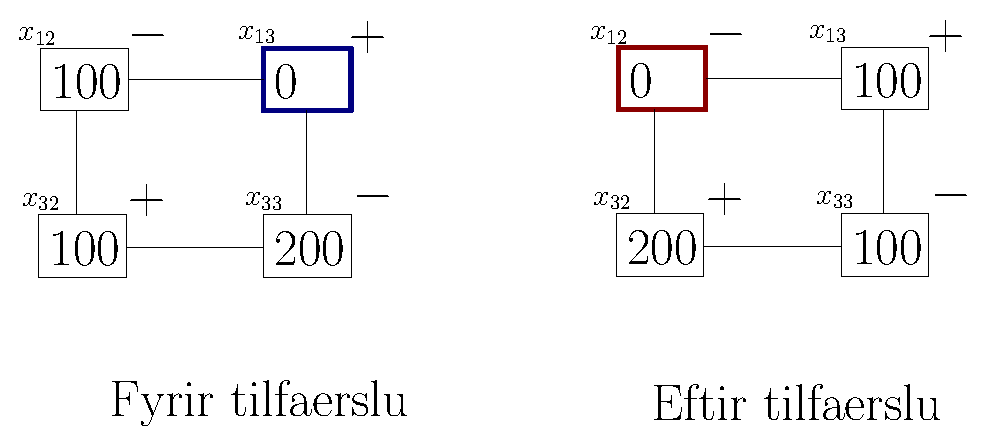
\includegraphics[width=0.6\columnwidth]{figs/flutn_bestun_hringras.eps}
\end{center}
Sjáum að $x_{12}$ fer úr grunni.
\end{enumerate}

\item[Fasi 2 -- ítrun \#2] Upphafstaflan er:
\begin{center}
\[ \begin{array}{cccr|cr|cr|crcc}
 & & \multicolumn{8}{c}{\mbox{Smásalar}} \\ \cline{3-10}
 & & \multicolumn{2}{|c|}{S1} & \multicolumn{2}{|c|}{S2} & \multicolumn{2}{|c|}{S3}& \multicolumn{2}{|c|}{S4} & s_i \\ \cline{2-11}
\multicolumn{1}{c|}{\multirow{8}{*}{\begin{sideways}Vöruhús\end{sideways}}} 
& \multicolumn{1}{|c|}{\multirow{2}{*}{V1}} &   & \scriptscriptstyle{\fbox{12}}&    & \scriptscriptstyle{\fbox{13}} & & \scriptscriptstyle{\fbox{4}}& & \scriptscriptstyle{\fbox{6}} & \multicolumn{1}{|c|}{\multirow{2}{*}{500}}  \\ 
& \multicolumn{1}{|c|}{                  } & \pscirclebox{400} & & &    &\pscirclebox{100} &   & & & \multicolumn{1}{|c|}{}\\ \cline{2-11}
& \multicolumn{1}{|c|}{\multirow{2}{*}{V2}} &   & \scriptscriptstyle{\fbox{6}}&    & \scriptscriptstyle{\fbox{4}} & & \scriptscriptstyle{\fbox{10}}& & \scriptscriptstyle{\fbox{11}} & \multicolumn{1}{|c|}{\multirow{2}{*}{700}}  \\ 
& \multicolumn{1}{|c|}{                  } &  &    & \pscirclebox{700}&    & & &&   & \multicolumn{1}{|c|}{}\\ \cline{2-11}
& \multicolumn{1}{|c|}{\multirow{2}{*}{V3}} &   & \scriptscriptstyle{\fbox{10}}&    & \scriptscriptstyle{\fbox{9}} &  & \scriptscriptstyle{\fbox{12}} & & \scriptscriptstyle{\fbox{4}} & \multicolumn{1}{|c|}{\multirow{2}{*}{800}} \\ 
& \multicolumn{1}{|c|}{                  } &   &    & \pscirclebox{200}&    & \pscirclebox{100}&   & \pscirclebox{500}& & \multicolumn{1}{|c|}{\multirow{2}{*}{}}\\ \cline{2-11}
&  \multicolumn{1}{c|}{d_j}& \multicolumn{2}{|c|}{400} & \multicolumn{2}{|c|}{900} & \multicolumn{2}{|c|}{200} &\multicolumn{2}{|c|}{500} & \\ \cline{3-10}
\end{array}
\]
\end{center}
 Síðan er haldið áfram eins og áður (gerið sjálf).
\end{description}
\end{lausn}
\newpage
\section{Gjaldgengar lausnir fyrir flutningsverkefni}
Norð-vestur aðferð horfir alveg framhjá $c_{ij}$ gildum og því getur upphafslausn verið langt frá bestu lausn sem kallar á margar ítranir í fasa 2.

\subsection{Aðferð lægsta kostnaðar}
\ath{Aðferð lægsta kostnaðar} (e. minimum cost criterion)\footnote{Sjá dæmi 8.2-4, bls. 350-1 í H\&L.} gefur yfirleitt betri upphafslausn en norð-vestur aðferð.
\begin{lausn}[á dæmi \ref{daemi:vorusmabilar}] Finnum upphafslausn með aðferð lægsta kostnaðar. 

\[ \begin{array}{cccr|cr|cr|crcc}
 & & \multicolumn{8}{c}{\mbox{Smásalar}} \\ \cline{3-10}
 & & \multicolumn{2}{|c|}{S1} & \multicolumn{2}{|c|}{S2} & \multicolumn{2}{|c|}{S3}& \multicolumn{2}{|c|}{S4} & s_i \\ \cline{2-11}
\multicolumn{1}{c|}{\multirow{8}{*}{\begin{sideways}Vöruhús\end{sideways}}} 
& \multicolumn{1}{|c|}{\multirow{2}{*}{V1}} &   & \scriptscriptstyle{\fbox{12}}&    & \scriptscriptstyle{\fbox{13}} & & \scriptscriptstyle{\fbox{4}}& & \scriptscriptstyle{\fbox{6}} & \multicolumn{1}{|c|}{\multirow{2}{*}{\cancel{500}\;\cancel{300}\;0}}  \\ 
& \multicolumn{1}{|c|}{                  } & \pscirclebox{300} &&& & \pscirclebox{200}&    & & & \multicolumn{1}{|c|}{}\\ \cline{2-11}
& \multicolumn{1}{|c|}{\multirow{2}{*}{V2}} &   & \scriptscriptstyle{\fbox{6}}&    & \scriptscriptstyle{\fbox{4}} & & \scriptscriptstyle{\fbox{10}}& & \scriptscriptstyle{\fbox{11}} & \multicolumn{1}{|c|}{\multirow{2}{*}{\cancel{700}\;0}}  \\ 
& \multicolumn{1}{|c|}{                  } &  &    & \pscirclebox{700}&    & & &&   & \multicolumn{1}{|c|}{}\\ \cline{2-11}
& \multicolumn{1}{|c|}{\multirow{2}{*}{V3}} &   & \scriptscriptstyle{\fbox{10}}&    & \scriptscriptstyle{\fbox{9}} &  & \scriptscriptstyle{\fbox{12}} & & \scriptscriptstyle{\fbox{4}} & \multicolumn{1}{|c|}{\multirow{2}{*}{\cancel{800}\;\cancel{300}}} \\ 
& \multicolumn{1}{|c|}{                  } &    \pscirclebox{100}&    & \pscirclebox{200}& &&  & \pscirclebox{500}& & \multicolumn{1}{|c|}{\multirow{2}{*}{\cancel{100}\;0}}\\ \cline{2-11}
&  \multicolumn{1}{c|}{d_j}& \multicolumn{2}{|c|}{\cancel{400}\;\cancel{300}\;0} & \multicolumn{2}{|c|}{\cancel{900}\;\cancel{200}\;0} & \multicolumn{2}{|c|}{\cancel{200}\;0} &\multicolumn{2}{|c|}{\cancel{500}\;0} & \\ \cline{3-10}
\end{array}
\]
Sjáum að $z=12000$, þ.e. finnur bestu lausn (\emph{fyrir tilviljun}) sem fæst staðfest í fasa 2.
\end{lausn}

\subsection{\ath{Aðferð Vogel}}
Fyrir sérhverja óútstrikaða línu/dálk reiknast \emph{mismunur} minnsta og næst minnsta kostnaðar. Finnum línu/dálk með mesta mismun. 
%Næsta breyta inn í grunn svarar til lægsta kostnaðar í viðkomandi\footnote{sem ekki er búið að stroka út} línu/dálki.
Veljum sem næstu grunnbreytu $x_{ij}$ sem er með minnsta óútstrikað $c_{ij}$ í línu eða dálki sem er með mesta mun. 

\begin{lausn}[á dæmi \ref{daemi:vorusmabilar}] Finnum upphafslausn með aðferð Vogels. 
\[ \begin{array}{cccr|cr|cr|crcc}
 & & \multicolumn{8}{c}{\mbox{Smásalar}} \\ \cline{3-10}
 & & \multicolumn{2}{|c|}{S1} & \multicolumn{2}{|c|}{S2} & \multicolumn{2}{|c|}{S3}& \multicolumn{2}{|c|}{S4} & s_i \\ \cline{2-11}
\multicolumn{1}{c|}{\multirow{8}{*}{\begin{sideways}Vöruhús\end{sideways}}} 
& \multicolumn{1}{|c|}{\multirow{2}{*}{V1}} &   & \scriptscriptstyle{\fbox{12}}&    & \scriptscriptstyle{\fbox{13}} & & \scriptscriptstyle{\fbox{4}}& & \scriptscriptstyle{\fbox{6}} & \multicolumn{1}{|c|}{\multirow{2}{*}{\cancel{500}\;\cancel{300}\;0}}  \\ 
& \multicolumn{1}{|c|}{                  } &&&&& \pscirclebox{200} & & \pscirclebox{300}&    & \multicolumn{1}{|c|}{}\\ \cline{2-11}
& \multicolumn{1}{|c|}{\multirow{2}{*}{V2}} &   & \scriptscriptstyle{\fbox{6}}&    & \scriptscriptstyle{\fbox{4}} & & \scriptscriptstyle{\fbox{10}}& & \scriptscriptstyle{\fbox{11}} & \multicolumn{1}{|c|}{\multirow{2}{*}{\cancel{700}\;0}}  \\ 
& \multicolumn{1}{|c|}{                  } &  &    & \pscirclebox{700}&    & & &&   & \multicolumn{1}{|c|}{}\\ \cline{2-11}
& \multicolumn{1}{|c|}{\multirow{2}{*}{V3}} &   & \scriptscriptstyle{\fbox{10}}&    & \scriptscriptstyle{\fbox{9}} &  & \scriptscriptstyle{\fbox{12}} & & \scriptscriptstyle{\fbox{4}} & \multicolumn{1}{|c|}{\multirow{2}{*}{\cancel{800}\;\cancel{600}}} \\ 
& \multicolumn{1}{|c|}{                  } &   \pscirclebox{400}&    & \pscirclebox{200}&  && & \pscirclebox{200}& & \multicolumn{1}{|c|}{\multirow{2}{*}{\cancel{400}\;0}}\\ \cline{2-11}
&  \multicolumn{1}{c|}{d_j}& \multicolumn{2}{|c|}{\cancel{400}\;0} & \multicolumn{2}{|c|}{\cancel{900}\;\cancel{200}\;0} & \multicolumn{2}{|c|}{\cancel{200}\;0} &\multicolumn{2}{|c|}{\cancel{500}\;\cancel{200}\;0} & \\ \cline{3-10}
\end{array}
\]
\vspace{5cm}

Sjáum að $z=12000$, þ.e. finnur bestu lausn (\emph{fyrir tilviljun}) sem fæst staðfest í fasa 2.
\end{lausn}




\subsection{\ath{Russel} regla}
Reiknum fyrir allar óútstrikaðar línur $i$ og dálka $j$:

$$\bar{u}_i = \max_{i\in \tiny{\mbox{ óútstr. dálkur }}}c_{ij} ~~~~~~~ \bar{v}_j = \max_{j\in \tiny{\mbox{ óútstr. lína }}}c_{ij}$$
$$\Delta_{ij}=c_{ij}-\bar{u}_i-\bar{v}_j$$
Næsta grunnbreyta er sú sem hefur minnsta $\Delta_{ij}$.

\begin{aths}Sjá dæmi á bls. 342, tafla 8.18, í H\&L. \end{aths}

\begin{daemi}[Flutningsverkefni í \athsub{\textsc{MathProg}}{\texttt{transport.mod}}]\hspace{.1cm}
 \lstinputlisting{../glpk/transport.mod}
\end{daemi}
Keyrum \textsc{glpk} á eftirfarandi hátt úr skelinni:
\begin{lstlisting}[language=bash]
hei2@Helga:~/IDN401G/$ glpsol -m transport.mod -o transport.sol
\end{lstlisting}
Lesum lausnina úr skjalinu \texttt{transport.sol}, sem reynist vera 
$$\begin{array}{lll}x_{S,NY}=0, & x_{S,C}=300,& x_{S,T}=0,\\ x_{SD,N}=325,& x_{SD,C}=0,& x_{SD,T}=275,\end{array}\quad\mbox{ með } z=\$ 153,675.$$


\section{Úthlutunarverkefni}
\ath{Úthlutunarverkefni} (e. assignment problem) er eins og flutningaverkefni þar sem öll framboð og allar
eftirspurnir eru $1$, þ.e.a.s.
$$\min_{\vec{x}} z = \sum_{i=1}^m\sum_{j=1}^n c_{ij}x_{ij}$$
þar $c_{ij}$ er kostnaður við að úthluta frá $i$ til $j$. Skorðurnar eru:
$$\sum_{j=1}^n x_{ij} = 1 ~~~ \mbox{og} ~~~ \sum_{i=1}^m x_{ij} = 1$$
fyrir  $i=1,\ldots,m$ og $j=1,\ldots,n$ og $x_{ij}\ge 0$ fyrir öll $i$ og $j$.

\begin{description}
 \item[Dæmi um hagnýtingar]\hspace{.1cm}
\begin{itemize}
 \item Úthluta verkum á vélar,
 \item Úthluta verkefnum á starfsmenn,
 \item Raða flugvélum á flugleiðir.
\end{itemize}
\end{description}

\begin{daemi}[Dæmi á bls. 334 í H\&L -- örlítið breytt\footnote{Hér er gert ráð fyrir að verkum er raðað á vélar, en í bókinni er gert ráð fyrir að raða vélum á staðsetningar.}]\label{daemi:verkvelar} Í verksmiðju einni þarf að vinna þrjú mismunandi verk \emph{samtímis}. Verkin má finna á fjórum mismunandi vélum. Kostnaður\footnote{Kostnaður gæti t.d. endurspeglað tíma vélar.} við tiltekið verk er háður því hvar það er unnið.
\[ \begin{array}{|l|cccc|} \hline &\textrm{Vél }1&\textrm{Vél }2&\textrm{Vél }3&\textrm{Vél }4\\ \hline
\textrm{Verk }1&13&16&12&11\\
\textrm{Verk }2&15&-&13&20\\
\textrm{Verk }3&5&7&10&6 \\ \hline
   \end{array}\]
\begin{aths}Verk 2 kemur ekki til greina á vél 2.\end{aths}
Finna á hagkvæmustu pörun milli véla og verka þannig að kostnaður sé lágmarkaður. 
\end{daemi}
\begin{samepage}
\begin{lausn}G.r.f. að eftirfarandi gildi:
\begin{enumerate}
 \item Fjöldi verka = fjöldi véla $=n$.
 \item Sérhver vél vinnur nákvæmlega eitt verk.
 \item Sérhvert verk er unnið á nákvæmlega einni vél.
 \item Kostnaður við að vinna verk $i$ á vél $j$ er $c_{ij}$.
 \item Finna hvernig á að úthluta verkum á vélar þ.a. kostnaður er lágmarkaður.
\end{enumerate}
Höfum fjögur verk, en einungis þrjár vélar. Bætum við \emph{gervivél} t.þ.a. koma verkefninu yfir á rétt form:
\[ \begin{array}{|l|cccc|} \hline &\textrm{Vél }1&\textrm{Vél }2&\textrm{Vél }3&\textrm{Vél }4\\ \hline
\textrm{Verk }1&13&16&12&11\\
\textrm{Verk }2&15&M&13&20\\
\textrm{Verk }3&5&7&10&6 \\ 
\textrm{Verk }4&0&0&0&0 \\ \hline
   \end{array}\quad\mbox{þar sem }M\textrm{ er stór tala.}\]
Ákvarðanabreyturnar eru 
$$ x_{ij}=\Big\{\begin{array}{cl} 1 & \textrm{ef verk }i\textrm{ er unnið á vél }j \\ 0 & \textrm{annars}\end{array}$$
Viljum leysa
$$ \min_{\vec{x}} z=\sum_{i=1}^n\sum_{j=1}^n c_{ij}x_{ij}$$
m.t.t. sk.
\begin{eqnarray*}
\sum_{j=1}^n x_{ij} = 1 && i\in\{1,\ldots,n\}\\
\sum_{i=1}^n x_{ij} = 1 && j\in\{1,\ldots,n\}\\ 
x_{ij}=0\vee 1 &&(\star)
\end{eqnarray*}
\begin{aths}Þetta er ekki hefðbundið línulegt bestunarverkefni vegna heiltöluskorðunnar $(\star)$.\end{aths}
Fáum jafngilt verkefni m.þ.a. slaka á heiltölukröfunni og setja í stað $x_{ij}\geq0$, þ.e.
$$ \min_{\vec{x}} z=\sum_{i=1}^n\sum_{j=1}^n c_{ij}x_{ij}$$
m.t.t. sk.
\begin{eqnarray*}
\sum_{j=1}^n x_{ij} = 1 && i\in\{1,\ldots,n\}\\
\sum_{i=1}^n x_{ij} = 1 && j\in\{1,\ldots,n\}\\ 
x_{ij}\geq 0 &&\forall i,j
\end{eqnarray*}
Þetta er flutningsverkefni með $n=m$ og $s_i=d_j=1$. 
\begin{aths}Eiginleiki slíkra verkefna er að ef $s_i$ og $d_j$ eru heiltölur þá er besta lausn heiltölulausn. Þess vegna verða $x_{ij}$ annaðhvort 0 eða 1 í bestu lausn á úthlutunarverkefnum.
\end{aths}
\end{lausn}
\end{samepage}
\subsection{Ungverska aðferðin}
\athsup{Ungverska aðferðin}{Úthlutunarverkefni} (e. Hungarian method) er lausnaraðferð sem er sérsniðin fyrir úthlutunarverkefni. Aðferðin byggir á því að draga má fasta frá sérhverri línu eða dálki án þess að besta lausn breytist, þ.e. 
$$\tilde{c}_{ij}=c_{ij}-p_i-q_j$$
því 
\begin{eqnarray*}
 z'&=& \sum_{i=1}^n\sum_{j=1}^n\tilde{c}_{ij}x_{ij}=\sum_{i=1}^n\sum_{j=1}^n \left(c_{ij}-p_i-q_j\right)x_{ij}\\
 &=& \sum_{i=1}^n\sum_{j=1}^n c_{ij}x_{ij}-\sum_{i=1}^n p_i \underbrace{\sum_{j=1}^nx_{ij}}_{=1}-\sum_{i=1}^n q_j\underbrace{\sum_{j=1}^nx_{ij}}_{=1}\\
&=& z\underbrace{-\sum_{i=1}^n p_i -\sum_{i=1}^n q_j}_{\textrm{fasti}}
\end{eqnarray*}

\begin{samepage}
\begin{description}
 \item[\athsub{Reiknirit}{Ungverska aðferðin} fyrir ungversku aðferðina]\hspace{.1cm}
 \begin{enumerate}[label=Skref \arabic{*}]
  \item Finna minnsta gildi í hverri línu, $p_i$,  og draga það frá öllum stökum í línunni.
  \item Finna minnsta gildi í hverjum dálki, $q_j$, og draga það frá öllum stökum í dálkinum.
  \item\label{ungv:aftur} $0$-stökin koma til greina sem besta úthlutun: 
 \begin{enumerate}
  \item Finna fyrstu línu með nákvæmlega einu $0$. Merkja með $\square$. Strika út viðkomandi dálka. 
  \item Meðhöndla óútstrikuðu dálka á sama máta, merkja núllreit með $\square$ og strika út viðkomandi línur.  
  \end{enumerate}
  Ef fjöldi útstrikaða lína $=n$ þá er besta lausn fundin. Hætta.
  \item Finna minnsta óútstrikaða stakið. Ef það er $>0$ draga það frá öllum óútstrikuðum stökum, leggja það síðan við þau stök þar sem tvær línur skerast. Aftur í \ref{ungv:aftur}.
  \item (Minnsta stak er 0) Velja eitthvað óútstrikað 0, merkja það með $\square$ og strika út þau núll sem eftir standa í tilsvarandi línu og dálki. \begin{aths}Hér geta verið margar jafngóðar lausnir.\end{aths} Endurtaka fyrir þau óútstrikuðu núll sem eftir standa. Stoppa.
 \end{enumerate}
\begin{aths} Ef reitur inniheldur $M$, þá er það látið halda sér.\end{aths}
\end{description}
\end{samepage}



\begin{lausn}[Ungverska lausnaraðferðin á dæmi \ref{daemi:verkvelar}] 
Lítum á minnsta stakið í hverri línu/dálki:
\[ \begin{array}{|l|cccc|c|} \hline \textrm{verk }i/\textrm{vél }j &\textrm{Vél }1&\textrm{Vél }2&\textrm{Vél }3&\textrm{Vél }4 & \min_i \textrm{ verk } i\\ \hline
\textrm{Verk }1&13&16&12&11 & 11\\
\textrm{Verk }2&15&M&13&20 & 13 \\
\textrm{Verk }3&5&7&10&6 & 5\\ 
\textrm{Verk }4&0&0&0&0 & 0\\ \hline
\min_j \textrm{ vél }j& 0 & 0 & 0 & 0 &\\\hline 
   \end{array}\]
\begin{description}
 \item[Skref 1] Drögum frá minnsta gildið frá öllum línum, og fáum
\[ \begin{array}{|l|cccc|} \hline \textrm{verk }i/\textrm{vél }j &\textrm{Vél }1&\textrm{Vél }2&\textrm{Vél }3&\textrm{Vél }4 \\ \hline
\textrm{Verk }1&2&5&1&0 \\
\textrm{Verk }2&2&M&0&7  \\
\textrm{Verk }3&0&2&5&1 \\ 
\textrm{Verk }4&0&0&0&0 \\ \hline
   \end{array}\]
\item[Skref 2] Óþarft, því minnsta gildið frá öllum dálkum er 0.
\item[Skref 3] 
\[ \begin{array}{|l|cccc|} \hline \textrm{verk }i/\textrm{vél }j &\textrm{Vél }1&\textrm{Vél }2&\textrm{Vél }3&\textrm{Vél }4 \\ \hline
\textrm{Verk }1&2&5&1&\fbox{0} \\
\textrm{Verk }2&2&M&\fbox{0}&7  \\
\textrm{Verk }3&\fbox{0}&2&5&1 \\ 
\textrm{Verk }4&0&\fbox{0}&0&0 \\ \hline
   \end{array}\]
Besta lausn er strax fundin, og lesum úr töflunni:

\[ \begin{tabular}{lll} Verk 1 &$\rightarrow$& Vél 4\\Verk 2 &$\rightarrow$& Vél 3\\Verk 3 &$\rightarrow$& Vél 1\end{tabular}
\quad\mbox{ með } z^*=5+13+11=29.\]
\begin{aths}Vél 2 er ónotuð.\end{aths}
\end{description}
\end{lausn}

\begin{daemi}[Giftingar]\label{daemi:gifting}Hjónabandsmiðlunin \textsc{MIR} sérhæfir sig í rússneskum konum og íslenskum sjómönnum. Kúnnahópurinn saman\-stendur af fjórum konum og fjórum körlum. Eftir að hafa tekið persónuleikapróf fást eftir\-farandi \emph{hamingjugildi} $h_{ij}$ milli kvennanna og karlanna:
\[ \begin{array}{|l|cccc|}\hline & \textrm{Fannar} & \textrm{Gunnar} & \textrm{Hilmar} & \textrm{Ingi} \\ \hline
    \textrm{Anastasiya}  & 7 & 5 & 8 & 2 \\
    \textrm{Borislava} & 7 & 8 & 9 & 4 \\
    \textrm{Dunya} & 3 & 5 & 7 & 9 \\
    \textrm{Elena} & 5 & 5 & 6 & 7 \\ \hline 
   \end{array}\]
Hvernig væri best að para framtíðar hjónaefnum? 
\end{daemi}
\begin{lausn}Þar sem við höfum ekki enn séð hvernig á að leysa heiltöluverkefni, þá til einföldunar skulum við g.r.f. að sjómennirnir eru tilbúnir að deila. Látum því $x_{ij}$ tákna hlutfalls þess tíma sem kona $i$ eyðir með manni $j$.

Úthlutunarverkefnið snýst um að hámarka hamingju, 
$$ \max_{\vec{x}} z=\sum_{i=1}^4\sum_{j=1}^4 h_{ij}x_{ij}$$
m.t.t. sk.
\[\begin{array}{lcc}
\textrm{Konur eyða bara tíma með mönnum}  & \sum_{j=1}^4 x_{ij}=1 & i\in\{1,...,4\}\\
\textrm{Menn eyða bara tíma með konum}  & \sum_{i=1}^4 x_{ij}=1 & j\in\{1,...,4\}\\
\textrm{Enginn er einn í ellinni} & x_{ij}\geq 0   
  \end{array}\]
Reikniritið okkar g.r.f. lágmörkun, breytum því hamingju í kostnað skv. $$c_{ij}=9-h_{ij}$$ því hæsta hamingjugildið er 9. Kostnaðartaflan verður:
\[ \begin{array}{|l|cccc||c|}\hline & \textrm{F} & \textrm{G} & \textrm{H} & \textrm{I} & \min\\ \hline
    \textrm{A} & 2 & 4 & 1 & 7 & 1\\
    \textrm{B} & 2 & 1 & 0 & 5 & 0\\
    \textrm{D} & 6 & 4 & 2 & 0 & 0\\
    \textrm{E} & 4 & 4 & 3 & 2 & 2 \\ \hline 
   \end{array}\]

Beitum nú ungverska reikniritinu:
\begin{description}
 \item[Skref 1] Drögum frá minnsta gildið frá hverri línu:
\[ \begin{array}{|l|cccc|}\hline & \textrm{F} & \textrm{G} & \textrm{H} & \textrm{I} \\ \hline
    \textrm{A} & 1 & 3 & 0 & 6\\
    \textrm{B} & 2 & 1 & 0 & 5 \\
    \textrm{D} & 6 & 4 & 2 & 0 \\
    \textrm{E} & 2 & 2 & 1 & 0  \\ \hline \hline
    \min & 1&1&1&0 \\ \hline
   \end{array}\]
 \item[Skref 2] Drögum frá minnsta gildið frá hverjum dálki:
\[ \begin{array}{|l|cccc|}\hline & \textrm{F} & \textrm{G} & \textrm{H} & \textrm{I} \\ \hline
    \textrm{A} & 0 & 2 & 0 & 6\\
    \textrm{B} & 1 & 0 & 0 & 5 \\
    \textrm{D} & 5 & 3 & 2 & 0 \\
    \textrm{E} & 1 & 1 & 1 & 0  \\ \hline 
   \end{array}\]
\item[Skref 3]Lína $D$ hefur nákvæmlega eitt núll í dálki $I$, merkjum það með $\square$ og strikum því dálk $I$ út.
  Dálkur $F$ hefur nákvæmlega eitt núll í línu $A$, merkjum með $\square$ og strikum því línu $A$ út.
Eins fer núllið í dálki $G$ inn í grunn, og lína $B$ strikuð út.   
\[ \begin{array}{|l|cccc|}\hline & \textrm{F} & \textrm{G} & \textrm{H} & \textrm{I} \\ \hline
    \textrm{A} & \fbox{0} & 2 & 0 & 6\\
    \textrm{B} & 1 & \fbox{0} & 0 & 5 \\
    \textrm{D} & 5 & 3 & 2 & \fbox{0} \\
    \textrm{E} & 1 & 1 & 1 & 0  \\ \hline 
   \end{array}\]
\item[Skref 4]Minnsta óútstrikaða stakið er $1>0$, drögum það frá óútstrikuðum stökum og leggjum við þau stök þar sem tvær línur skerast, þ.e.
\[ \begin{array}{|l|cccc|}\hline & \textrm{F} & \textrm{G} & \textrm{H} & \textrm{I} \\ \hline
    \textrm{A} & \fbox{0} & 2 & 0 & 7\\
    \textrm{B} & 1 & \fbox{0} & 0 & 6 \\
    \textrm{D} & 4 & 2 & 1 & \fbox{0} \\
    \textrm{E} & 0 & 0 & 0 & 0  \\ \hline 
   \end{array}\]
\item[Skref 2]Dálkur $H$  hefur nákvæmlega eitt núll, merkjum það með $\square$ og strikum því dálk $E$ út.
\[ \begin{array}{|l|cccc|}\hline & \textrm{F} & \textrm{G} & \textrm{H} & \textrm{I} \\ \hline
    \textrm{A} & \fbox{0} & 2 & 0 & 7\\
    \textrm{B} & 1 & \fbox{0} & 0 & 6 \\
    \textrm{D} & 4 & 2 & 1 & \fbox{0} \\
    \textrm{E} & 0 & 0 & \fbox{0} & 0  \\ \hline 
   \end{array}\]
   Fjöldi grunnbreyta $=n$, svo besta lausn er fundin og heildarhamingjan er $7+8+9+6=30$.
\begin{aths}Í bestu lausn eyðir fólkið öllum sínum tíma með ein\-hverjum af gagnstæða kyni (sjá \href{http://en.wikipedia.org/wiki/Hall's_marriage_theorem}{\emph{marriage theorem}}).\end{aths}

\end{description}
\end{lausn}

\begin{lausnSYND}[á dæmi \ref{daemi:gifting} með \athsub{\textsc{MathProg}}{\texttt{assignment.mod}}]
Nú ætlum við að sýna forsjáshyggju og aðskilja stærðfræðilega líkanið frá gögnunum, ef ske kynni að aðrar hjónabandsmiðlanir vilja nýta sérfræðiráðgjöf okkar á úthlutun kvenna á karla.

\newpage
Almennt líkan á úthlutun kvenna á karla er eftirfarandi:
\lstinputlisting{../glpk/assignment.mod}
Því næst skulum við skrifa skrá sem heldur einungis utan um gögnin fyrir þessa tilteknu hjónabandsmiðlun MIR:
\lstinputlisting{../glpk/MIR.dat} 
Keyrum \textsc{glpk} á eftirfarandi hátt úr skelinni:
\begin{lstlisting}[language=bash]
hei2@Helga:~/IDN401G/$ glpsol -m assignment.mod -d MIR.dat -o MIR.sol
\end{lstlisting}
Lesum bestu lausnina úr skelinni (því við notuðum $\texttt{display}$ skipunina) 
$$\begin{tabular}{lll}Anastasiya & $\Longleftrightarrow$ & Hilmar \\
   Borislava & $\Longleftrightarrow$ & Gunnar  \\
   Dunya&$\Longleftrightarrow$ &Ingi \\
   Elena&$\Longleftrightarrow$ &Fannar
  \end{tabular} $$
Úttaks-skráin \texttt{MIR.sol} sýnir að heildarhamingjan er $z^*=30$.
\begin{aths}Sjáum að \textsc{glpk} gefur ekki sömu lausn og ungverska lausnar\-aðferðin, en markfallsgildið er að engu að síður hið sama. 
\end{aths}


\end{lausnSYND}



\section{Almenn flutningsverkefni}
Höfum nú þegar kynnst flutninga- og úthlutunarverkefnum, en þau eru dæmi um netverkefni sem hægt er að leysa með línulegri bestun.
\begin{figure}[h!]
\centering
 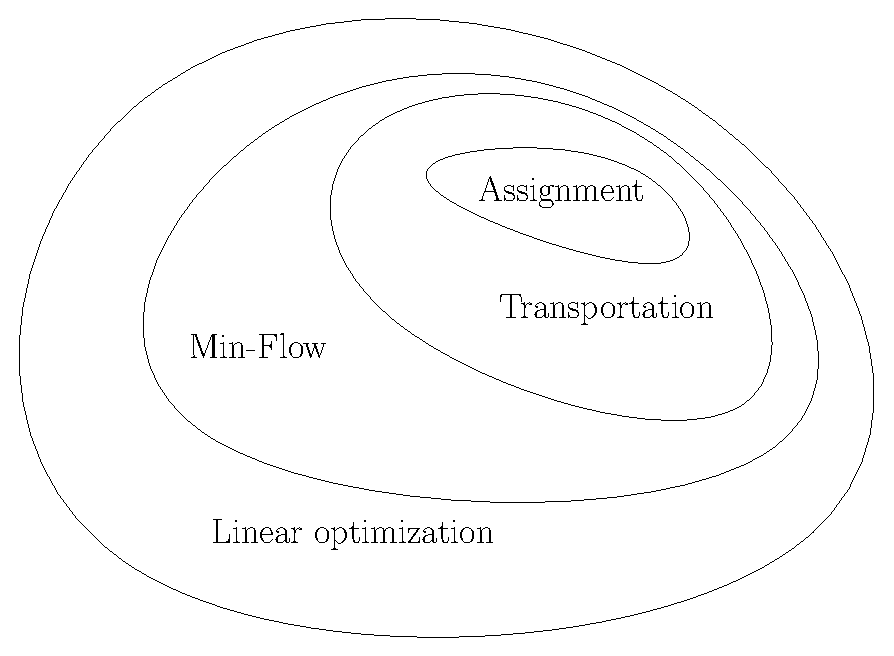
\includegraphics[width=0.6\columnwidth]{figs/types_of_networkproblems.eps}
\end{figure}

Netverkefni eru fjölbreytt bestunarverkefni með margskonar hag\-nýtingu til dæmis:
\begin{itemize}
 \item samgöngukerfum, 
\item fjarskiptum, 
\item fjármálum, 
\item verkefnastjórnun
\item vöru\-stjórnun.
\end{itemize}

\begin{comment}
\begin{itemize}
\item Mikil þróun á aðferðum til að leysa netlíkön.
\item Nokkur sérstök netverkefni:
  \begin{itemize}
  \item stysta leið (e. shortest path),
  \item léttasta spanntré (e. minimum spanning tree)
  \item mesta flæði (e. max flow)
  \item minnsta kostnaðar flæði (e. minimum cost flow)
  \item PERT (program evaluation and review technique) og\\ CPM
  (critical path method).
  \end{itemize}
\end{itemize}
\end{comment}

Mörg hagnýt netverkefni falla undir línulega bestun og má oft finna reiknirit sem eru \emph{sérsniðin} að einstökum tegundum verkefna. En áður en lengra er haldið þarf nokkur hugtök úr \ath{netafræði} (e. graph theory).

\section{Nokkur hugtök úr netafræði}

\begin{description}
 \item[\athsup{Net}{netafræði}] (e. network / graph) er safn af \athsup{hnútum}{netafræði} (e. node) eða punktum og \athsup{leggjum}{netafræði} (e. edges), hver leggur tengir tvo hnúta.
\begin{center} \includegraphics[width=0.37\columnwidth]{figs/network.eps} \end{center}

\begin{center}
\begin{tabular}{|l|lll|}
\hline
Dæmi: & Hnútur & Leggur & Flæði \\ \hline
Vegakerfi & gatnamót & götur  & bílar \\
Flug & flugvellir &  flugleiðir & flugvélar \\
Samskiptakerfi & hnútpunktar & rásir & skeyti\\
Vatnsdreifikerfi & dælur & pípur & vatn \\
Afbrot & krimmar & tengsl krimma & (á ekki við) \\
\hline
\end{tabular}
\end{center}
 \item[\athsup{Stefnt net}{netafræði}] eða örvanet (e. directed network) er net þar sem leggirnir hafa stefnu, þeir eru \athsup{stefndir leggir}{netafræði} eða \athsup{örvar}{netafræði} (e. arc / directed edge). Ef flæði er í báðar áttir, þá er hann óstefndur. %Net sem hefur aðeins stefnda leggi kallast stefnt net.
 \begin{center} \includegraphics[width=0.24\columnwidth]{figs/directed.eps} \end{center}
 \item[\athsup{Leið}{netafræði}] (e. path) er runa af leggjum sem tengir tvo hnúta (örvar sem snúa í rétta átt í örvaneti)
 \begin{center} 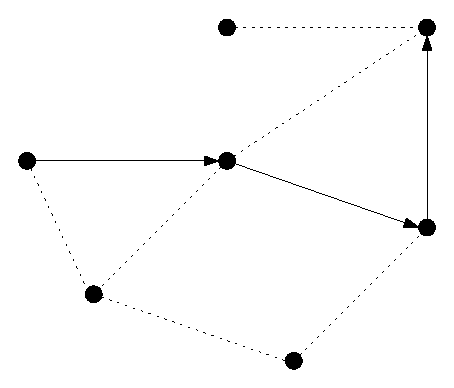
\includegraphics[width=0.27\columnwidth]{figs/path.eps} \end{center}
 \item[\athsup{Rás}{netafræði}] eða hringrás (e. circuit) er leið sem tengir hnút við sjálfan sig (e. cycle / circuit) 
 \begin{center} 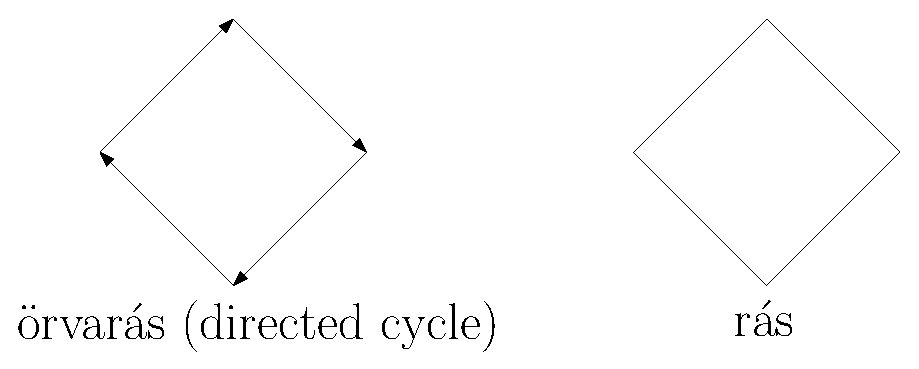
\includegraphics[width=0.6\columnwidth]{figs/cycle.eps} \end{center}
 \item[\athsup{Samhangandi net}{netafræði}] (e. connected graph) er net þar sem til er leið milli sérhverja tveggja punkta í netinu.
 \item[\athsup{Tré}{netafræði}] (e. tree) Tré er samhangandi net sem inniheldur enga hringi, rásalaust net (eða hlutanet).
 \begin{center} \includegraphics[width=0.6\columnwidth]{figs/tree.eps} \end{center}
 \item[\athsup{Spanntré}{netafræði}] (e. spanning tree) í neti er tré sem tengir alla hnúta netsins. %Í neti með $n$ hnúta er alltaf $n-1$ leggur í hverju spanntré.
 \begin{center} 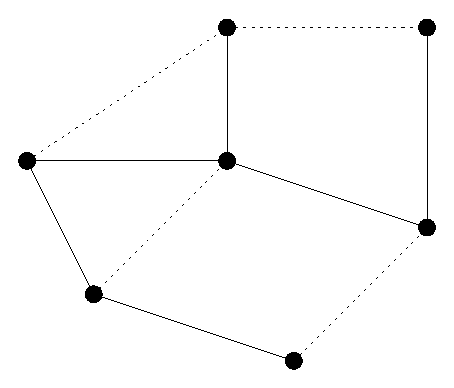
\includegraphics[width=0.3\columnwidth]{figs/spantree.eps} \end{center}
 \item[\athsup{Flæðinet}{netafræði}] (e. flow network) 
 \begin{itemize}
    \item Hverjum legg tengist \athsup{flæði}{netafræði} (oft eru það ákvörðunarbreytur verkefnisins).
    \item Flæðinet hefur \athsup{burðargetu}{netafræði} (e. capacity).
    \item Hnútur með innflæði í net er \athsup{upphafsstaður}{netafræði}, \athsup{upp\-spretta}{netafræði} eða \athsup{lind}{netafræði}.
    \item Þar sem flæðir út úr neti er \athsup{ós}{netafræði}, \athsup{svelgur}{netafræði} eða \athsup{áfangastaður}{netafræði} (e. sink, destination).
    \item Hnútar án inn- eða útflæðis eru \athsup{millihnútar}{netafræði} (e. transshipment node).
  \end{itemize}
 \begin{center} 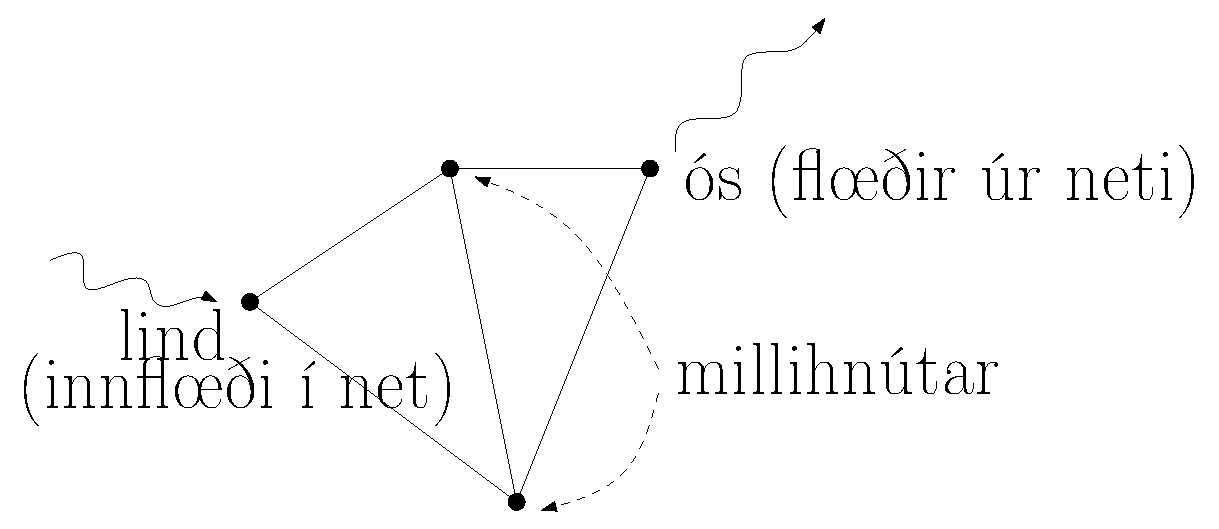
\includegraphics[width=0.6\columnwidth]{figs/flownet.eps}\end{center}
\item{\ath{Stysta leið} (e. shortest path)}
\begin{itemize}
\item Óstefnt, samhangandi net.
\item Upphafspunktur (e. source) og endapunktur (e. sink).
\item Fyrir hvern legg höfum við \emph{fjarlægð} 
\item Markmið: Finna leið sem lágmarkar fjarlægð frá upphafspunkti í endapunkt.
\end{itemize}
\end{description}

\section{Stysta leið}
\begin{daemi}[Seervada garður]\label{daemi:seervada}Finna skal stystu leið á milli upphafsstaðs $O$ og áfangastaðs $T$ gefið:
\begin{center}
  \includegraphics[width=0.7\columnwidth]{figs/seervada.eps}
\end{center}
%\[\begin{array}{lrl}
% \textrm{Stysta leið:} & \min  z = \sum_{i=1}^7 \sum_{j=1}^7 c_{ij}x_{ij}\\
% \textrm{Upphafsstaður:} & \sum_{j=1}^7 x_{Oj} - \sum_{i=1}^7 x_{iO} & =  1\\
% \textrm{Millistaður:} & \sum_{j=1}^7 x_{kj} - \sum_{i=1}^7 x_{ik}  &=  0 \\
% \textrm{Áfangastaður:} & \sum_{j=1}^7 x_{Tj} - \sum_{i=1}^7 x_{iT}  &=  -1
%\end{array}\]
%þar sem $k \in \{A,B,C,D,E\}$, og $x_{ij} \ge 0$ fyrir öll $ i,j \in \{O,A,B,C,D,E,T\}$.
\end{daemi}

Línulegt bestunarverkefni fyrir stystu leið hefur ákvarðanabreytur
\[ x_{ij}=\Big\{\begin{array}{ll} 1 & \textrm{ef leggur }i\to j\textrm{ er á leiðinni}\\ 0 & \textrm{annars}\end{array}\]
Höfum gefna fasta
\begin{eqnarray*}
d_{ij} &=& \textrm{vegalengd milli } i \textrm{ og } j\\
\mathcal{V}&=& \textrm{ mengi hnúta, t.d. } \mathcal{V}=\{O,A,B,C,D,E,T\}\\
\mathcal{E}&=& \textrm{ mengi leggja, t.d. } \mathcal{E}=\{(O,A),(O,C),...,(D,T),(E,T)\}\\
\end{eqnarray*}
Viljum lágmarka 
$$ \min_{\vec{x}} \sum_{(i,j)\in \mathcal{E}} d_{ij}x_{ij} $$
m.t.t. sk.
$$ \underbrace{\overbrace{\sum_{k:(k,i)\in \mathcal{E}}x_{ki}}^{\textrm{innflæði í }i}-\overbrace{\sum_{j:(i,j)\in \mathcal{E}}x_{ij}}^{\textrm{útflæði úr } i}}_{\textrm{nettóflæði}}=\Bigg\{\begin{array}{clc} 1 & \textrm{ef }i=O & \textrm{(lind)}\\-1 & \textrm{ef }i=T& \textrm{(svelgur)}\\0&\textrm{annars}& \textrm{(millinóður)}\end{array}\quad \forall\; i\in \mathcal{V}$$
$$x_{ij}\geq0$$
\begin{aths}Eiginleiki verkefnisins er að í bestu lausn eru öll $x_{ij}=0\vee1$. \end{aths}

\begin{description}
 \item[Afbrigði]\hspace{.1cm}
 \begin{itemize}
  \item Finna minnsta \emph{tíma} sem röð verka tekur.
  \item Finna minnsta \emph{kostnað} við röð verka.
 \end{itemize}
 \item[Notkun]\hspace{.1cm}
 \begin{itemize}
  \item Bestun á samgöngukerfum (t.d. stysta leið milli tveggja staða í borginni).
  \item Tölvunet: stysta leið (um internetið ) frá tölvu $Alice$ til $Bob$.
  \item Stundum má tækla flókin verkefni í aðgerðagreiningu m.þ.a. leysa runu af stystu leiðar verkefnum.
 \end{itemize}

\end{description}



\begin{comment}
\begin{lausn}[á stystu leið dæmis \ref{daemi:seervada} með \athsup{\textsc{matlab}}{Stysta leið}]
Það sem vantar að gera í línulega bestunarverkefninu er að eyða út leggjum sem eru ekki til, t.d. $x_{AC}$. Við getum annað hvort sett $c_{AC} = M$ (stór tala) eða sett $x_{AC} = 0$ (þ.e.a.s. tekið $x_{AC}$ út):
\lstinputlisting{seervada_shortestpath.m}
\begin{center}
  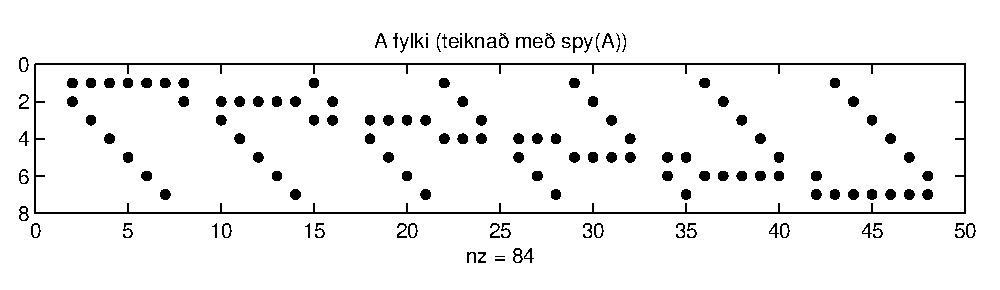
\includegraphics[width=0.7\columnwidth]{figs/seervada-f1.eps}
\end{center}
\end{lausn}
\end{comment}
\newpage
\begin{lausnSYND}[á stystu leið dæmis \ref{daemi:seervada} með \athsub{\textsc{MathProg}}{\texttt{spp.mod}}]\mbox{Almennt} líkan fyrir stystu leið í \textsc{MathProg} er eftirfarandi:
\lstinputlisting[language=awk]{../glpk/spp.mod}
Gagnaskráin fyrir Seervada garðinn er 
\lstinputlisting[language=awk]{../glpk/seervada.dat}\label{seervada.dat}
Keyrum \textsc{glpk} úr skelinni, 
\begin{lstlisting}[language=bash]
hei2@Helga:~/IDN401G/$ glpsol -m spp.mod -d seervada.dat --wcpxlp cplex.skra  
\end{lstlisting}
Lesum úr skelinni (því við notuðum \texttt{printf} skipunina í \texttt{spp.mod}) að leggir í grunni eru 
$$1\leftrightarrow2,\; 2\leftrightarrow3,\; 3\leftrightarrow5,\; 5\leftrightarrow7 \mbox{ með } z^*=13.$$ 
eða með réttum rithætti
$$O\rightarrow A \rightarrow B \rightarrow D \rightarrow T$$ 

Á bak við tjöldin breytti \textsc{glpk} líkanamálinu \textsc{MathProg} í skorður sem það skilur. Hægt er að sjá hvernig þær nákvæmlega litu út með að líta á \textsc{cplex} keyrsluskránna:
\lstinputlisting{../glpk/cplex.skra}
\end{lausnSYND}

\subsection{Reiknirit fyrir stystu leið}
\begin{enumerate}[label=Skref \arabic{*}]
\item \athsup{Leystur hnútur}{Stysta leið} (e. solved node):  Stysta leið í hnútinn frá upphafs\-hnút er þekkt. Í byrjun er upphafshnúturinn eini leysti hnúturinn.
%Byrjið í upphafspunkti. Setjið fjarlægð frá upphafspunkti $=$ núll, þetta kallast merkt fjarlægð, upp\-hafspunkturinn kallast nú leystur hnútur.
\item \label{skref:0} Finnið næsta hnút með:
\begin{enumerate}[label=(\roman{*})]
\item\label{skref1} Skoðið alla óleysta hnúta sem eru tengdir leystum hnút
  (þetta eru kandídatar)
\item\label{skref2} Reiknið fjarlægð að upphafspunkti með því að leggja
fjarlægð í hnút við merkta fjarlægð
\item\label{skref3} Kandídatinn með minnstu fjarlægð frá upphafspunkti verður næsti leysti hnútur (ef jafntefli, leysið þá fyrir báða hnúta)
\end{enumerate}
\item Aftur í \ref{skref:0} uns áfangastaður er leystur hnútur.
\item Stysta leið finnst með því að vinna sig afturábak frá áfangastað.
\end{enumerate}

\begin{lausn}[á stystu leið Seervada úr dæmi \ref{daemi:seervada} með reikniriti]

{\renewcommand{\arraystretch}{1.5} \renewcommand{\tabcolsep}{0.2cm}
{\footnotesize\[
\begin{array}{|p{.5cm}p{1.2cm}cccp{1.3cm}p{1.2cm}|}
\hline
 \textrm{Ítrun } $n$ &
 \textrm{Leystir hnútar }&
 \textrm{\ref{skref:0}\ref{skref1} }&
 \textrm{\ref{skref:0}\ref{skref2} }&
\textrm{\ref{skref:0}\ref{skref3} }& 
 \textrm{Lágmarks fjarlægð} &
 \textrm{Síðasta tenging} \\ 
\hline
1 & O & A & 2 & A & 2 & OA \\ 
\hline
2 & O & C & 4 & C & 4 & OC \\ 
3 & A & B & 2+2=4 & B & 4 & AB \\ 
\hline
 & A & D & 2+7=9 &  &  &  \\ 
4 & B & E & 4+3=7 & E & 7 & BE \\ 
 & C & E & 4+4=8 &  &  &  \\ 
\hline
 & A & D & 2+7=9 &  &  &  \\ 
5 & B & D & 4+4=8 & D & 8 & BD \\ 
 & E & D & 7+1=8 & D & 8 & ED \\ 
\hline
6 & D & T & 8+5=13 & T & 13 & DT \\ 
 & E & T & 7+7=14 &  &  &  \\ 
\hline
\end{array}\]
}}
Allir hnútar eru nú \emph{leystir}. Finnum stystu leið m.þ.a. rekja okkur til baka
$$ T\leftarrow D\leftarrow E \leftarrow B \leftarrow A \leftarrow O$$
eða 
$$ T\leftarrow D\leftarrow B \leftarrow A \leftarrow O$$
með vegalengd $z^*=13$ 
\begin{aths}Fundum tvær \emph{jafn} góðar bestu lausnir. Tökum eftir að \textsc{glpk} fann aðeins seinni lausnina.
\end{aths}


\end{lausn}
\newpage
\subsection{Dijkstra reiknirit}
\lstinputlisting{../matlab/dijkstra.m}

\begin{daemi}[á stystu leið Seervada  úr dæmi \ref{daemi:seervada} með Dijkstra]\hspace{.1cm}
\begin{lstlisting}
>> O=1;A=2;B=3;C=4;D=5;E=6;T=7;
>> c = inf*ones(n,n);
>> c(O,A) = 2; c(A,O) = 2; c(O,B) = 5; c(B,O) = 5; c(O,C) = 4; c(C,O) = 4; c(A,B) = 2; c(B,A) = 2; c(A,D) = 7; c(D,A) = 7; c(B,C) = 1; c(C,B) = 1; c(C,E) = 4; c(E,C) = 4; c(B,E) = 3; c(E,B) = 3; c(B,D) = 4; c(D,B) = 4; c(D,E) = 1; c(E,D) = 1; c(T,E) = 7; c(E,T) = 7; c(T,D) = 5; c(D,T) = 5; 
>> [path, fmin] = shortestpath(c, 1, 7);
tempdist =
     0   Inf   Inf   Inf   Inf   Inf   Inf
tempdist =
   Inf     2     5     4   Inf   Inf   Inf
tempdist =
   Inf   Inf     4     4     9   Inf   Inf
tempdist =
   Inf   Inf   Inf     4     8     7   Inf
tempdist =
   Inf   Inf   Inf   Inf     8     7   Inf
tempdist =
   Inf   Inf   Inf   Inf     8   Inf    14
path =
     1     2     3     5     7
fmin =
    13
>> labels = 'OABCDET'; labels(path)
ans =
OABDT
\end{lstlisting}
\end{daemi}

\section{\ath{Léttasta spanntré}}
\begin{description}
 \item[\ath{Spanntré}  ] Til er leið á milli allra para af hnútum í tréinu.
 \item[\ath{Léttasta spanntré}  (e. minimum spanning tree)] Spanntré þannig að heildar\-lengd leggja er sem minnst.
 \item[Hagnýting]\hspace{.1cm}
\begin{itemize}
 \item Hönnun á samskiptakerftum (ljósleiðaranet)
 \item Samgöngukerfi (lestar, vegir)
 \item Háspennukerfi
 \item Pípukerfi
\end{itemize}
 \item[Inntak í reiknirit]\hspace{.1cm}
 \begin{enumerate}
  \item[$\mathcal{H}$] Safn hnúta
  \item[$\mathcal{L}$] Safn \emph{mögulegra} leggja
  \item[$\mathcal{D}$] Lengd/þyngd leggja í $\mathcal{E}$.
 \end{enumerate}
 \item[Reiknirit]\hspace{.1cm}
 \begin{enumerate}[label=Skref \arabic{*}]
  \item Velja hnút af handahófi 
  \item\label{skref:minspan:aftur} Velja \emph{léttasta legg} sem ekki er þegar kominn í tréið og sem myndar ekki hringrás með leggjunum sem eru þar fyrir. Bætum þessum legg í tréið.
  \item Aftur í \ref{skref:minspan:aftur} þangað til netið inniheldur $n-1$ leggi.
 \end{enumerate}
 \begin{aths}Þetta kallast \ath{gráðugt} (e. greedy) reiknirit. Hægt að stilla upp sem LP -- en ekki alveg eins einfalt.\end{aths}
\end{description}

\begin{lausn}[Léttasta spanntré fyrir Seervada úr dæmi \ref{daemi:seervada}]\hspace{.1cm}
\begin{center}
  \includegraphics[width=0.7\columnwidth]{figs/seervada-tree.eps}
\end{center}
Lægsti heildarkostnaður $2+2+1+3+1+5=14$.
\end{lausn}


\subsection{Samantekt}
\begin{description}
 \item[Stysta leið] Finnur stystu \emph{vegalengd} milli tveggja hnúta.
 \item[Léttasta spanntré] Finnur stystu \emph{heildarvegalengd} milli allra para af hnútum.
\end{description}

\newpage

\section{Hámarksflæði}
Hér er markmiðið að senda sem \ath{mesta flæði} (e. max flow) í gegnum netið. Aðferð
til að leysa þetta verkefni er að:

Viljum finna \ath{hámarksflæði} (e. max flow) frá $A$ til $B$ fyrir eitthvað tiltekið net, t.d.
\begin{center}
  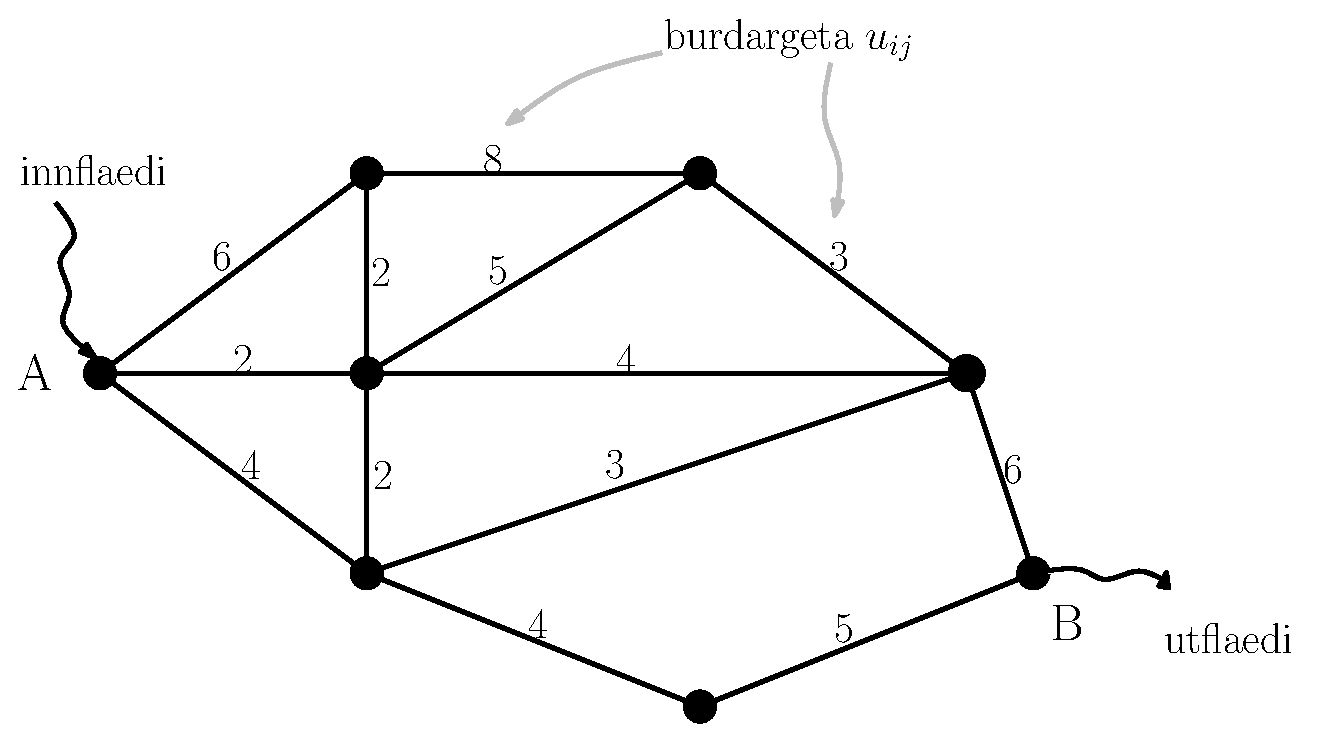
\includegraphics[width=0.7\columnwidth]{figs/maxflow.eps}
\end{center}
Getum gert það m.þ.a.
\begin{itemize}
 \item Nota sérsniðið reiknirit, t.d. \ath{aðferð aukandi vega} (bls. 374--9 í H\&L)
 \item Nota reiknirit fyrir \ath{minnsta kostnaðar flæði} (sjá síðar)
 \item Stilla upp línulegu bestunarlíkani og leysa með Simplex.
\end{itemize}
Fyrir línulegt bestunarlíkan sem hámarkar flæði, látum $\mathcal{H}=\{1,...,n\}$ tákna safn $n$ hnúta og $\mathcal{L}$ tákna safn leggja. Ákvarðanabreytur eru $x_{ij}=$ flæði á legg $i\to j$. Leysum 
$$ \max_{x_{ij}\in\mathcal{L}} d $$ 
m.t.t. sk.
\begin{eqnarray*}
\sum_{i:(i,k)\in\mathcal{L}} x_{ik} - \sum_{j:(k,j)\in\mathcal{L}} x_{kj} &=& 0 \quad \mbox{fyrir }k\in\mathcal{H}\setminus\{1,n\} \\ 
\sum_{j:(1,j)\in\mathcal{L}} x_{1j} &=& s \\ 
\sum_{i:(i,n)\in\mathcal{L}} x_{in} &=& d \\
x_{ij} &\leq& u_{ij} \\
x_{ij}&\geq&0 
\end{eqnarray*}

%\begin{center}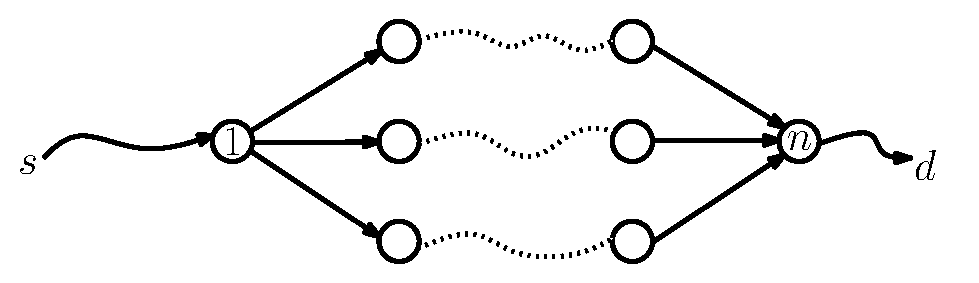
\includegraphics[width=0.75\columnwidth]{figs/maxflow_thm.eps}\end{center}
\begin{samepage}
\begin{aths}\begin{itemize}
\item Fyrstu þrjár skorðurnar hafa í för með sér að $s=d$.
\item Til er afbrigði af hámarksflæði, þ.a. $x_{ij}\geq l_{ij}$.
\end{itemize}
\end{aths}
\end{samepage}
\subsection*{Nokkur dæmi um hagnýtingu}
 \begin{itemize}
  \item Hámarka flæði vatns eða olíu í pípukerfum.
  \item Hámarka flæði faratækja (lestir, bílar) um samgöngumannvirki.
 \item Velja einhverja leið af handahófi í gegnum netið.
\item Finna minnstu burðagetu leiðarinnar og senda það magn í
  gegnum netið. Burðagetan minnkar um þetta magn fyrir þessa leið.
\item Ítrum áfram þangað til engin nýtanleg leið með 
  burðagetu finnst. Þá erum við komin í hámark.
\end{itemize}

\begin{daemi}[Mesta flæði]
Finnum mesta flæði fyrir Seervada (dæmi \ref{daemi:seervada}). 
\end{daemi}

\begin{lausnSYND}[með \athsub{\textsc{MathProg}}{\texttt{maxflow.mod}}]Almennt líkan fyrir mesta flæði er eftirfarandi:
\lstinputlisting[language=Awk]{../glpk/maxflow.mod} 
Höfum gagnaskrá fyrir Seervada garðinn á bls. \pageref{seervada.dat}. 
Keyrum því \textsc{glpk} á eftirfarandi hátt úr skelinni, og lesum bestu lausn beint úr skelinni:
\begin{lstlisting}[language=bash]
hei2@Helga:~/IDN401G/$ glpsol -m maxflow.mod -d seervada.dat
========================================================
Maximum flow from node 1 to node 7 is 11

Starting node   Ending node   Arc capacity   Flow in arc
-------------   -----------   ------------   -----------
            1             2              2             2
            1             4              4             4
            1             3              5             5
            2             5              7             2
            3             5              4             2
            3             6              3             3
            4             6              4             4
            5             7              5             4
            6             7              7             7
========================================================
Model has been successfully processed
\end{lstlisting}
\begin{figure}[h!]
 \begin{center}
  \includegraphics[width=0.7\columnwidth]{figs/seervada_maxflow.eps}
 \end{center}\caption{Hámarksflæði fyrir Seervada garðinn}
\end{figure}
\end{lausnSYND}
\newpage
\begin{daemi}[Nálgun á fylkjum]Viljum nálga eftirfarandi fylki af fleytitölum í heiltölur
\[\begin{array}{ccc}
& & \sum \\
&\begin{bmatrix}
   3.14 & 6.8 & 7.3 \\
   9.6 & 2.4 & 0.7 \\
   3.6 & 1.2 & 6.5 
 \end{bmatrix} & \begin{matrix} 17.24 \\ 12.7 \\ 11.3\end{matrix} \\ 
\sum & \begin{matrix} 16.34 & 10.4 & 14.5\end{matrix}
\end{array}\]
\end{daemi}
\begin{lausn}Setjum upp nálgun fylkisins sem net þ.a. við getum hámarkað flæðið, þ.e.
 \begin{center}
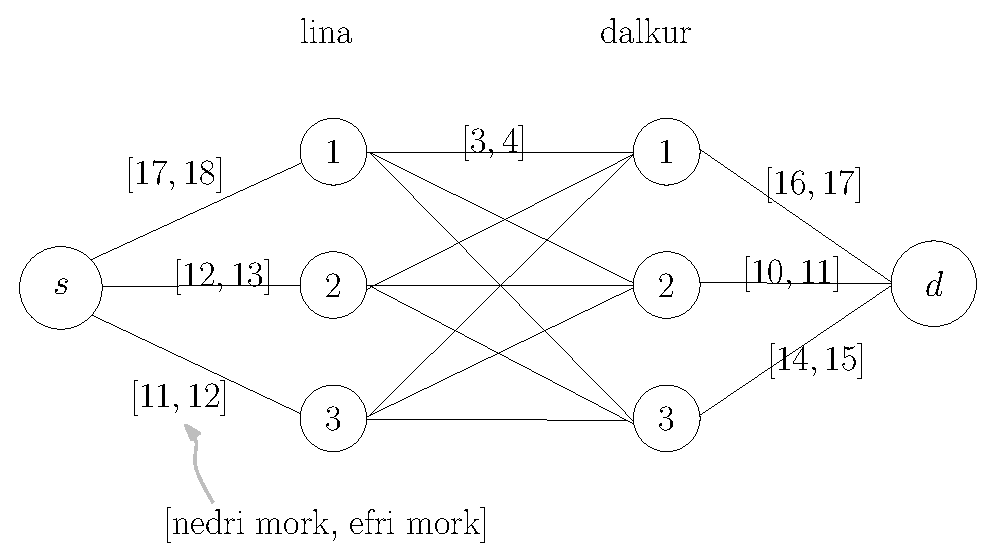
\includegraphics[width=0.75\columnwidth]{figs/maxflow_matrix.eps}
\end{center}
þar sem burðargetan er skorðuð af neðri og efri mörkum á heiltölunálgun gildanna. Besta lausn reynist vera 
\[\begin{array}{ccc}
& & \sum \\
&\begin{bmatrix}
   3 & 7 & 7 \\
   10 & 2 & 1 \\
   3 & 1 & 7 
 \end{bmatrix} & \begin{matrix} 17  \\ 13 \\ 11\end{matrix} \\ 
\sum & \begin{matrix} 16 & 10 & 15\end{matrix}
\end{array}\]
\end{lausn}

\begin{daemi}[Gjaldeyrisbrask]Gengi nokkra gjaldmiðla
\[\begin{array}{c|cccc}\hline 
   &       \mbox{USD} & \mbox{TRY} & \mbox{AED} & \mbox{GBP} \\ \hline 
\mbox{USD} &-& 1.0883 & 3.6732 & 0.7004\\
\mbox{TRY} & 0.5921 &-& 2.1766 & 0.4148\\
\mbox{AED} &0.2722 & 0.4596 &-& 0.1906\\
\mbox{GBP} &1.4298 & 2.4130 & 5.2471 &-\\ \hline 
  \end{array}\]
Sjáum t.d. að $GBP\to TRY\to GBP$ gefur ávöxtun upp á $1.6883\cdot 0.5921=0.9996$ (tap) en $USD\to AED\to GBP\to USD$ gefur $\$0.0010$ í gróða á hvern dollar sem braskað er með.

Hvernig getum við fundið högnunartækifæri (e. arbitrage)?
\end{daemi}
\begin{lausn}
Látum $\mathcal{C}$ tákna mengi gjaldmiðla og $r_{ij}$ tákna gengi á milli gjaldmiðla $i$ og $j$. Ef við byrjum með $USD$ þá getum við \emph{leitað} að högnun m.þ.a. leysa
$$ \max d$$
m.t.t. sk.
\begin{eqnarray*}
 \sum_{j\in\mathcal{C},\;j\neq i} x_{ij}-\sum_{j\in\mathcal{C},\;j\neq i} x_{ji}r_{ji} = 0\quad\forall\;i\in\mathcal{C}\setminus\{USD\} \\
 f+\sum_{j\in\mathcal{C}\setminus\{USD\}} x_{USD,j}-\sum_{j\in\mathcal{C}\setminus\{USD\}} x_{j,USD}r_{j,USD}=1\\
f\leq 2,\quad x_{ij}\geq 0
\end{eqnarray*}
Sjáum að þetta er náskylt mesta flæðis verkefninu.

Besta lausn gefur ávöxtun $1.00143$ á dollar ef $USD\to GBP\to USD$ þ.e.a.s. við þurfum $\$683$ til þess að græða $\$1$.
\begin{aths}Gerðum ekki ráð fyrir þóknun.\end{aths}

\end{lausn}



\section{Flæði lægsta kostnaðar}
\ath{Flæði lægsta kostnaðar} (e. minimum cost flow) er nokkuð almennt verkefni, undir það fall m.a. stysta leið, mesta flæði og flutningsverkefni (sjá nánar 386--9 í H\&L). Til er hagkvæmt reiknirit sem kallast \ath{Netsimplex aðferðin}.

\subsection{Netsimplex aðferðin}
\ath{Netsimplex-aðferðin} er sérsniðin að minnsta kostnaðar flæðisverkefni. Hún byrjar á einhverri gjaldgengri spanntréslausn og rekur sig á milli slíkra lausna með  því að skipta út einum legg í hverju skrefi  þar til komið er í bestu lausn.
\begin{description}
 \item[Ákvörðunarbreytur]$x_{ij} = $ flæði í gegnum legg $i \rightarrow j$
 \item[Gögn]\hspace{.1cm}
\begin{itemize}
\item $c_{ij}$ kostnaður við flæði á legg $i\to j$
\item $u_{ij}$ \ath{burðargeta leggs} (e. arc capacity) fyrir legg $i\to j$
\item $b_i$ er heildarflæði í hnút $i$
\begin{itemize}
\item $b_i > 0$ ef hnútur $i$ er lind
\item $b_i < 0$ ef hnútur $i$ er svelgur
\item $b_i = 0$ ef hnútur $i$ er millihnútur
\end{itemize}
\end{itemize}
\end{description}
Línulegt verkefni sem lágmarkar heildarkostnað, summan er aðeins tekin yfir leggi sem eru til staðar:
$$\min_\vec{x} ~~  Z = \sum_{i=1}^{n}\sum_{j=1}^{n}c_{ij}x_{ij}$$
skorður fyrir hvern hnút $i\in\mathcal{H}$
$$\sum_{j\in \deg^-(i)} x_{ij}-\sum_{j\in\deg^+(i)}^n x_{ji}=b_i$$
og efra mark á ákvörðunarbreytum
$$0 \le x_{ij} \le u_{ij}$$

\begin{samepage}\begin{aths}Skilyrði fyrir að verkefnið hafi löglega lausn er \mbox{$\sum_{i\in\mathcal{H}} b_i = 0$}.
Ef $b_i$ og $u_{ij}$ eru allar heiltölur þá verða ákv.breyturnar ($\vec{x}^*$) líka heiltölur.
\end{aths}\end{samepage}

\begin{daemi}Höfum gefið eftirfarandi net:
\begin{center}
\includegraphics[width=0.9\columnwidth]{figs/netsimplex.eps} 
\end{center}
\end{daemi}


\begin{lausn}Beitum netsimplex-aðferðinni:
\begin{comment}
\begin{enumerate}[label=(\arabic{*})]
 \item Fyrsta grunnlausn 
  \begin{center}
  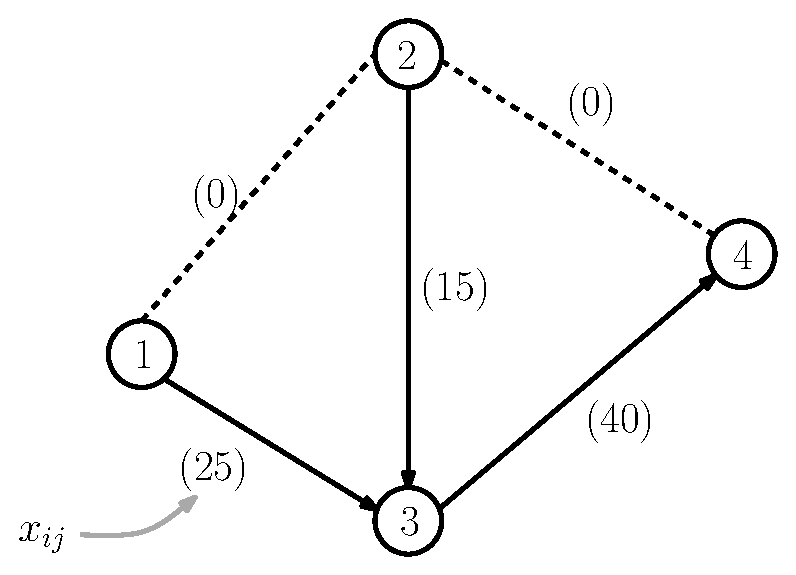
\includegraphics[width=0.6\columnwidth]{figs/netsimplexstart.eps}
  \end{center}
  \item %Ítrun 1
    Ef ör $1\to 2$ er bætt í tréð myndast hringrás og ef flæðið eftir $1\to 2$ er aukið um $\theta$ (það er 0) og flæði eftir öðrum örvum er aukið eða minnkað um $\theta$ og þá breytist $z$ um \[\Delta z = \sum_{(i,j)\in\mbox{hringrás}}c_{ij}(\pm\theta)=2\theta+8\theta-7\theta = 3\theta\quad\Rightarrow\;\frac{\partial z}{\partial \theta}=3\]
    Ef ör $2\to 4$ bætt við er $\frac{\partial z}{\partial \theta}=3-6-8=-11$. \linebreak 
    Nýr grunnur og lausn:
    \begin{center}
    \includegraphics[width=0.5\columnwidth]{figs/netsimplex-1.eps}
    \end{center}
    bætum ekki við ör $2\to 3$ því þá förum við aftur í upphafslausn.
  \item %Ítrun 2
Ör $1\to 2$ gefur $\Delta z = 2+3-6-7=-8$ og nýja flæðið breytist:\linebreak
\begin{center}
  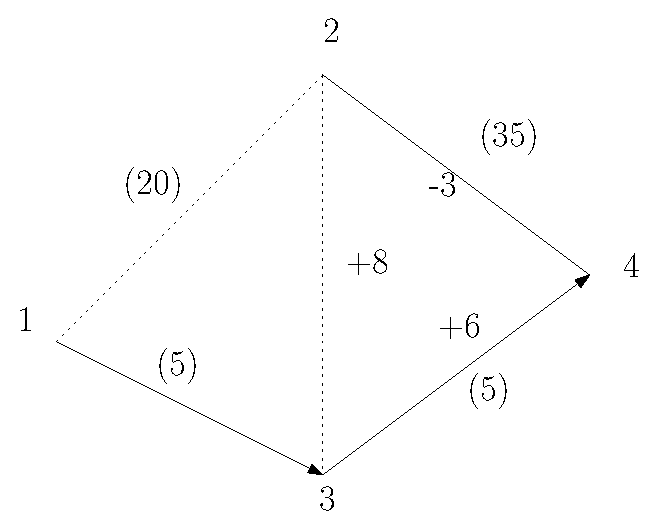
\includegraphics[width=0.5\columnwidth]{figs/netsimplex-2.eps}
\end{center}
Athugið að örin $1\to 2$ sem er í efri mörkum telst ekki vera í grunni. Hérna notum við \emph{upper bound} aðferðina og
skiptum út $x_{12}$ með \mbox{$u_{12} - y_{12}$} þar sem $0\le y_{12} \le u_{12}$ (lesið kafla 7.3 í H\&L).
\item %Ítrun 3
Ef flæðið eftir $2\rightarrow 3$ er aukið: $\Delta z = +8\theta+6\theta-3\theta = 11\theta$\linebreak
Ef flæðið eftir $1\rightarrow 2$ er minnkað um $\theta$: $\Delta z = -c_{12}\theta -c_{24}\theta+c_{34}\theta+c_{13}\theta=-2\theta-3\theta+6\theta+7\theta = 8\theta$ (þetta síðasta var í raun óþarfi  því við vorum  að bæta inn flæði eftir $1\rightarrow 2$ í 2. ítrun, en sýnir hvernig reiknað er ef ör sem er í efri mörkum  kæmi í grunn. \linebreak
Bæði $\Delta z >0$ svo besta lausn er fundin.
\end{enumerate}
\end{comment}
\end{lausn}








\newpage
\begin{daemi}[Minnsta kostnaðar flæði í \textsc{MathProg}]\hspace{.1cm}
\lstinputlisting{../glpk/mincostflow.mod}
\end{daemi}



\subsection{Samband minnsta kostnaðar og mesta flæðis}
Hægt er að nota \ath{min cost flow} lausnaraðferðir til þess að leysa \ath{max flow} verkefni. Hugsum okkur að við höfum max flow verkefni með eina lind (e. source), eina ós (e. sink) og nokkra hnúta (e. nodes) ásamt hámarksburðargetu leggja. Til að breyta þessu verkefni yfir í min cost flow verkefni þarf einungis að breyta þrennu:
\begin{enumerate}
\item Látum kostnaðinn $c_{ij}=0$ fyrir öll $i,j$ þ.e. setjum kostnað sérhvers leggs jafnt og núll.
\item Veljum nægilega stórt $\hat{F}$, sem á að tákna öruggt efra mark gjaldgengs flæðis í gegnum netið. Þ.e. setjum $\hat{F}$ á lindina og $-\hat{F}$ á ósina.
\item Búum til nýjan legg milli lindar og ósar, setjum á hann ótakmarkaða burðargetu og stóran kostnað $M$.
\end{enumerate}

Tökum eftir að lágmörkun kostnaðar þess verkefnis jafngildir að hámarka flæði í gegnum upphaflega netið. Því vissulega viljum við lágmarka flæðið sem fer í gegnum nýja legginn sem hefur mikinn kostnað, sem gerist einmitt þegar sent er sem mest flæði í gegnum upphaflega netið.



\section{\ath{Critical Path Method} (CPM)}
\begin{daemi}[Verkefnastjórnun] Lágmarka á tíma sem tekur að byggja  hús (sjá töflu bls. 400 og mynd bls. 402). 
Viljum vinna verkið á 40 vikum. Hvernig er hagkvæmast að gera það?
\end{daemi}
\begin{lausn}
Getum fundið sex mismunandi vegi í gegnum netið:
{\footnotesize
\begin{verbatim}
    * Start A B C D G H M Finish       Lengd: 40 vikur
    * Start A B C E H M Finish         Lengd: 31 vikur
    * Start A B C E F J K N Finish     Lengd: 43 vikur
    * Start A B C E F J L N Finish     Lengd: 44 vikur
    * Start A B C I J K N Finish       Lengd: 41 vika
    * Start A B C I J L N Finish       Lengd: 42 vikur
\end{verbatim}}
Sú lengsta tekur 44 vikur. Þetta er stysti tíminn sem verkið getur tekið (kostn. 4.55 milljónir).
\begin{quote} Verk á þessari leið eru \emph{flöskuhálsar} -- mikilvægt að þeim seinki ekki.
%Til að stytta tímann þurfum við að skoða þann veg og hvaða verkþátt er hægt að stytta. 
\end{quote}
Oft má flýta einstökum verkþáttum m.þ.a. auka við mannskap, vélar, tæki, meiri yfirvinnu o.s.frv. Af þessu hlýst viðbótarkostnaður. Ef öllum verk\-þáttum er flýtt einsog mögulegt er þá tekur verkið 28 vikur og kostnaður er 6.15 milljónir. 

Setjum upp línulegt bestunarverkefni:
\begin{description}
 \item[Ákvarðanabreytur]\hspace{.1cm}
\begin{description}
\item[$x_j$] tími sem verk $j$ er stytt um.
\item[$y_j$] upphafstími verks $j$.
\end{description}
\item[Gefið]\hspace{.1cm}
\begin{description}
 \item[$t_j$] tími sem tekur að vinna verk $j$.
 \item[$c_j$] kostnaður við að \emph{krassa} verki.
\end{description}
\end{description}
Vandamálið snýst því um að lágmarka 
$$ \min_{\vec{x},\vec{y}} z= \sum_{j\in\mathcal{H}} c_jx_j $$
m.t.t. sk.
\begin{eqnarray*}
 y_j\geq y_i+t_i-x_i &&\mbox{fyrir öll verk } i \mbox{ sem eru undanfarar }j\\
 y_{finish}\leq 40 \\ y_i\geq0 && 0\leq x_j\leq x_j^{\max} 
\end{eqnarray*}
\end{lausn}

 
\chapter{Heiltölubestun} \label{ch:ip}
\ath{Heiltölubestun} (e. integer programming) hefur margvíslega hagnýtingu í bestun.
Rifjum upp forsendur línulegrar bestunar 
\begin{enumerate}
  \item Engin óvissa í stikum líkansins (e. certainty)
  \item Skorður og markfall línuleg föll
  \item Deilanleiki ákvörðunarbreyta (e. devisibility) 
\end{enumerate}
Ef
\begin{enumerate}
  \item er ekki uppfyllt $\Rightarrow$ \ath{slembin bestun} (e. stochastic programming)
  \item er ekki uppfyllt $\Rightarrow$ \ath{ólínuleg bestun} (e. nonlinear programming)
  \item er ekki uppfyllt $\Rightarrow$ \ath{heiltölubestun} (e. integer programming)
\end{enumerate}

Í mörgum hagnýtum verkefnum er deilanleikaforsendan ógild eða hæpin forsenda. Sem dæmi má nefna bestun á vaktaplani þar sem ákvarðanabreytur svara til fjölda starfsmanna á vakt. Lausnir þar sem fjöldinn er ekki heiltölur hafa enga merkingu, hvernig á að túlka 1.5 starfsmenn?

Ef gildi ákvarðanabreyta í bestu lausn eru nálguð að næstu heiltölu getur nýja lausnin verið umtalsvert lakari en \emph{besta} heiltölulausn eða það sem verra er hún er ekki endilega gjaldgeng.

\begin{samepage}
\begin{daemi}\label{daemi:ip:myndr}Gjaldgenga svæðið afmarkað af skorðum verkefnisins er skyggt og svartir punktar eru gjaldgengar lausnir. Besta lausn línulega bestunarverkefnisins er $(\frac{3}{2},2)$. Aftur á móti eru rúnuðu lausnirnar annaðhvort $(1,2)$ eða $(3,2)$ -- báðar ógjaldgengar. 
\begin{center}
  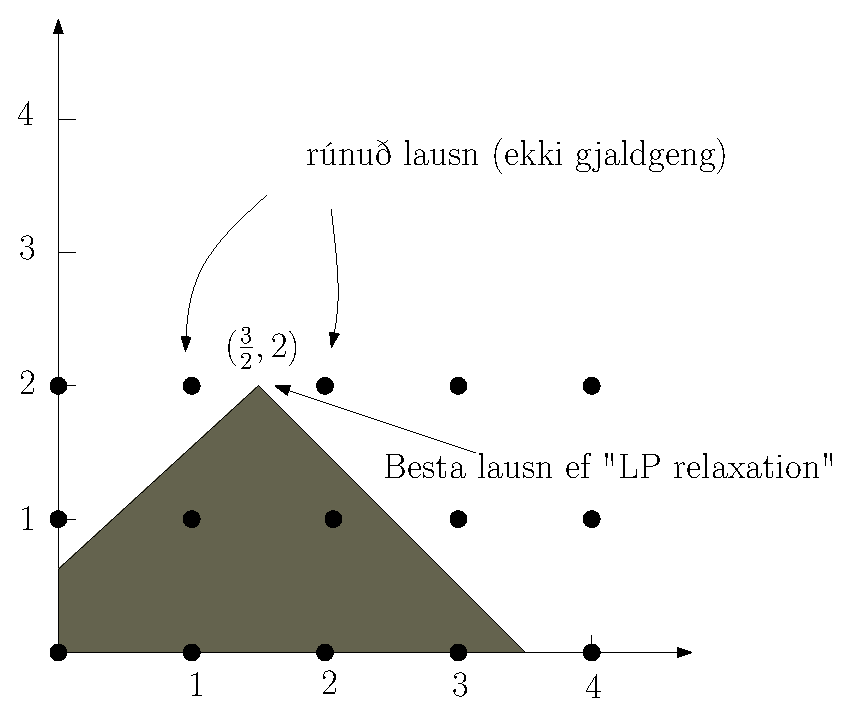
\includegraphics[width=0.7\columnwidth]{figs/relaxation.eps}
\end{center}
\end{daemi}
\end{samepage}

\begin{aths}Ef slakað er á kröfum ákvarðanabreytanna um að vera heiltölur í rauntölur, þá er talað um \ath{LP-tilslökun} (e. LP-relaxation).\end{aths}



\section{Tegundir bestunarlíkana}
Gerum greinarmun á eftirfarandi tegundum verkefna:
\begin{itemize}
\item Gerum ráð fyrir að föll séu línuleg og sleppum að taka fram \emph{línulega} heiltölubestun.
\item Þegar allar breytur í líkani eru heiltölubreytur kallast það \ath{heiltölubestun} (e. Integer Programming), IP. 
\item Ef sumar eru heiltölubreytur en aðrar samfeldar notum við \ath{blandaða heiltölubestun} (e. Mixed Integer Programming), MIP. 
\item Þegar við höfum \emph{binary} breytur sem aðeins geta tekið gildið 1 eða 0, þá höfum við \ath{tvíkostaverkefni} (e. Binary Integer Programming) BIP.
\end{itemize}

\begin{samepage}
\begin{aths}Verkefni þar sem taka þarf röð \emph{já--nei} ákvarðana má oft setja fram sem tvíkostaverkefni með 
$$ x_j=\Bigg\{\begin{array}{cl} 1 & \mbox{ef ákvörðun }j\mbox{ er tekin} \\ 0 & \mbox{annars}\end{array} $$  
\end{aths}
\end{samepage}

\begin{daemi}[Staðarval]\label{daemi:stadarval} Ákveða á hvort það á að byggja verksmiðju í $LA$ eða $SF$, eða jafnvel á báðum stöðum. Einnig er í \emph{athugun} hvort byggja eigi einn nýjan lager, og yrði hann annað hvort byggður í $SF$ eða $LA$. Einnig er skilyrði að það verði að vera verksmiðja þar sem lager er \mbox{byggður}. 
Eftirfarandi framlegðar- og kostnaðartölur liggja fyrir í ($\$10^6$)
\[
\begin{tabular}{|c|l|c|c|c|}
\hline
Nr.ákv. & Ákvörðun & Ákv.br. & Núvirtur hagnaður & Fjármagnsþörf \\
\hline
1 & Verksm. í $LA$ & $x_1$ & 9 & 6\\
2 & Verksm. í $SF$ & $x_2$ & 5 & 3 \\
3 & Lager í $LA$ & $x_3$ & 6 & 5\\
4 & Lager í $SF$ & $x_4$ & 4 & 2\\
\hline
 &              &      & Fjármagn til reiðu: & 10\\
\hline
\end{tabular}\]
Fjármagn er takmarkað og ákvarða þarf hvað eigi að byggja þannig að arðsemi sé hámörkuð.
\end{daemi}

\begin{lausn}Stærðfræðilegt líkan:
$$\max_\vec{x} z = 9 x_1 + 5 x_2 + 6 x_3 + 4 x_4$$
m.t.t. sk.:
\begin{eqnarray*}
  6 x_1 + 3 x_2 + 5 x_3 + 2 x_4 & \le & 10 \\
  x_3 &\le& x_1 \\
  x_4 &\le& x_2 \\
  x_3+x_4 &\le& 1\\
  x_j &\ge& 0 \\
  x_j &\le& 1 \\
  x_j & & \mbox{er heiltala} \\
  x_j & & \mbox{er tvíundarbreyta} \\
\end{eqnarray*}
\begin{equation*}
x_j = 
\begin{cases}
1 & \text{ ef ákvörðun er já,}  \\
0 & \text{ ef ákvörðun er nei.} \\
\end{cases}
\quad j=1,2,3,4.
\end{equation*}

\newpage
Leysum með \textsc{glpk} m.þ.a. setja
\begin{lstlisting}
  var x1, binary;
  var x2, binary;
  var x3, binary;
  var x4, binary;
\end{lstlisting}
Markfall og skorður eins og lýst er hér að ofan. Besta lausn er $x^*_1=x^*_2=1$, $x^*_3=x^*_4=0$ með $z^*=14$.

\end{lausn}

\subsection*{Dæmi um hagnýtingu tvíkostaverkefna}
Mörg verkefni tengd fjárfestingum eru svipaðs eðlis, þ.e. ákveða á hvort ráðast eigi í tilteknar fjárfestingar en ekki bara hversu mikið eigi að fjárfesta (hefðbundin línuleg bestun).
\begin{itemize}
  \item Fjárfestingar: Þegar ákveða á \emph{hvort} ráðast eigi í tilteknar framkvæmdir (sbr. dæmi \ref{daemi:stadarval}) en ekki bara \emph{hversu mikið} eigi að fjárfesta (hefðbundin línuleg bestun)
  \item Ákvarða \emph{hvar} á að byggja/opna nýja verksmiðju/verslun o.s.frv.
  \begin{eqnarray*}
    x_j&=&\Bigg\{\begin{array}{cl} 1 & \mbox{ef á að byggja á stað }j\\0 & \mbox{annars}\end{array}\\
  \end{eqnarray*}
  \item Samval hlutabréfa (e. portfolio optimization): Finna eignasafn sem lágmarkar áhættu m.v. tiltekna (vænta) ávöxtun og lágmarkar jafnframt kostnað við kaup og sölu (e. transaction costs). Tvær ákvarðanabreytur fyrir hvert (hluta)bréf:
  \begin{eqnarray*}
    y_j&=&\Bigg\{\begin{array}{cl} 1 & \mbox{ef bréf }j\mbox{ er keypt}\\0 & \mbox{annars}\end{array}\\
    x_j&=&\mbox{magn sem á að kaupa af bréfum }j
  \end{eqnarray*}
  \item Vöruútkeyrsla á sendibílum til viðskiptavina
  \begin{eqnarray*}
    x_{ij}&=&\Bigg\{\begin{array}{cl} 1 & \mbox{ef bíll }i\mbox{ fer til viðskiptavinar }j\\0 & \mbox{annars}\end{array}\\
  \end{eqnarray*}
  \item Sala á eignum: \emph{hvenær} á að selja t.þ.a. hámarka hagna
  \begin{eqnarray*}
    x_{ij}&=&\Bigg\{\begin{array}{cl} 1 & \mbox{ef eign }i\mbox{ er seld á tímabili  }j\\0 & \mbox{annars}\end{array}\\
  \end{eqnarray*}
  \item Flugrekstur (uppspretta marvíslegra bestunarverkefna): Úthlutun flugvéla á flugleiðir
  \begin{eqnarray*}
    x_{ij}&=&\Bigg\{\begin{array}{cl} 1 & \mbox{ef flugvél }i\mbox{ flýgur leið }j\\0 & \mbox{annars}\end{array}\\
  \end{eqnarray*}
  \item Lágmarka kostnað en uppfylla jafnframt kröfum um afköst.
\end{itemize}

\section{Skorður með tvíkostabreytum}
Með því að innleiða tvíkostabreytur má vinna með fjölbreyttari skorður en áður (þ.e. allar skorður uppfylltar).

\subsection{\ath{Annaðhvort--eða skorður}}
Annaðhvort þarf skorða $(1)$ eða skorða $(2)$ að gilda.
\begin{daemi}[Framhald af Wyndor úr dæmi \ref{wyndor:org}] Við höfum tvö aðföng til að nota í ákveðnum tilgangi og því þarf að virða magn sem til er af öðrum hvorum aðföngunum. Því þarf annaðhvort að gilda 
\[ 3 x_1 + 2 x_2  \le 18 \]
eða
\[ x_1 + 4 x_2  \le 16\]

\end{daemi}
\begin{lausn}Látum $M>0$ tákna einhverja stóra tölu svo skorðan skerði ekki lausnarrúmið. Jafngildar skorður eru
\begin{itemize}
  \item annaðhvort $\Bigg\{\begin{array}{rll} 3 x_1 + 2 x_2  &\le 18 \\ x_1 + 4 x_2  &\le 16+M & \quad\mbox{(alltaf uppfyllt)}\end{array}$
  \item eða~~~~~~~~~~~ $\Bigg\{\begin{array}{rll} 3 x_1 + 2 x_2  &\le 18+M& \quad\mbox{(alltaf uppfyllt)} \\ x_1 + 4 x_2  &\le 16 \end{array}$
\end{itemize}
Innleiðum nýja breytu $y\in\{0,1\}$ -- ákvörðunarbreyta. Þá fæst
\[ \begin{array}{rll} 3 x_1 + 2 x_2  &\le 18+My \\ x_1 + 4 x_2  &\le 16+M(1-y) \end{array}\]
\begin{aths} $y$ kallast \ath{aukabreyta} (e. auxiliary variable).\end{aths}
\end{lausn}

\subsection{$K$ af $N$ skorður eru með}
Hægt að útfæra \emph{annaðhvort--eða} skorður þannig að $K$ af $N$ skorðum séu með, þ.e. $K$ af $N$ skorðum eiga að halda.

\begin{daemi}\hspace{.1cm}
\begin{eqnarray*}
g_1(x_1,x_2,\ldots, x_n) &\le& b_1 + My_1\\
g_2(x_1,x_2,\ldots, x_n) &\le& b_2 + My_2\\
& \vdots & \\
g_m(x_1,x_2,\ldots, x_n) &\le& b_m + My_m\\
\sum_{i=1}^m y_i &=& N - K
\end{eqnarray*}
Þar sem $y_i$ er tvíundarbreytur þ.a. $y_i=\Bigg\{\begin{array}{cl}1 & \mbox{ef skorða er með}\\0 &\mbox{annars}\end{array}$.
\end{daemi}


\subsection{Föll með $N$ mögulegum gildum}
Oft geta föll tekið nokkur skilgreind gildi, t.d.
$$ f(x_1,...,x_n)=d_1~\mbox{eða}~d_2~\mbox{eða}~d_3~\mbox{eða}~\cdots$$
\begin{daemi}[Hlutir sem koma í kippum -- t.d. bjór] Höfum fall: $$ 3 x_1+ x_2 = 6 \mbox{ eða } 12 \mbox{ eða } 18$$\end{daemi}
 \begin{lausn}Þetta má setja upp sem:
\begin{eqnarray*}
3 x_1 + x_2 & = & 6 y_1 + 12 y_2 + 18 y_3 \\
y_1 + y_2 + y_3 & = & 1
\end{eqnarray*}
þar sem  $y_1, y_2, y_3$ eru tvíundarbreytur.
\end{lausn}

\subsection{Fastagjald}
Fastagjald ef ákveðin ákvörðunarbreyta er notuð.
\begin{daemi} Ef framleiða á ál þarf að gangsetja ofn. G.r.f. að kostnaður við að framleiða afurð $j$ sé 
$$f_j(x_j)=\Bigg\{\begin{array}{cl}k_j+c_jx_j & \mbox{ef } x_j>0\\0 &\mbox{annars}\end{array}$$
þar sem $k_j$ er fastur kostnaður vöru $j$ og $c_j$ er breytilegur kostnaður vöru $j$.

Viljum lágmarka heildarkostnað við framleiðsluna 
$$\min_{\vec{x}} z  =  \sum_{j=1}^N f_j(x_j)$$

\end{daemi}
\begin{lausn}Innleiðum aukabreytu $y_j\in\{0,1\}$ þ.a. $y_j=\Bigg\{\begin{array}{cl} 1 & \mbox{ef } x_j>0\\0 &\mbox{annars}\end{array}$. Þá fæst 
$$\min_{\vec{x}} z  =  \sum_{j=1}^N c_j x_j + \sum_{j=1}^N k_j y_j $$
m.t.t. sk. 
$$x_j \leq M y_j  $$
því að 
\[\begin{matrix}y_j=0 & \Rightarrow & x_j=0 \\y_j=1 & \Rightarrow & x_j>0 \end{matrix} \]
\begin{aths}Ef $x_j=0$, þá verður $y_j=0$ vegna þess að við erum að lágmarka $z$ og $k_j>0$.\end{aths}
\end{lausn}

\section{Lausnaraðferðir}
Mikil vinna við að þróa aðferðir til að leysa heiltölubestunarvandamál.

Fjöldi mögulegra heiltölulausna er endanlegur (sáum í dæmi \ref{daemi:ip:myndr} að þær væru 6 talsins). Er einfaldlega hægt að prófa allar mögulegar lausnir og velja síðan þá bestu? Nei! Fjöldi lausna vex \emph{mjög} hratt.

Fyrir tvíkosta verkefni með $n$ breytum er fjöldui mögulegra lausna $\leq 2^n$. Getum útilokað þær sem uppfylla ekki skorður.

\begin{daemi}[Veldisvísisvöxtur]Skoðum tímann sem tekur að prófa allar lausnir, gefið $m=n$ skorður, fyrir mismunandi gildi á $n$.
Fjöldi lausna sem má prófa á sek er u.þ.b. $3\cdot10^9$ með $3GHz$ tölvu:
\begin{center}
  \[\begin{array}{cll} n & 2^n & \mbox{tími} \\ \hline 
10 & 1024 \\
20 & \approx10^6 & 1~\mbox{sek}  \\
30 & \approx10^{9} & 20~\mbox{mín}\\
40 & \approx10^{12} & 27~\mbox{dagar}\\
50 & \approx10^{15} & 119~\mbox{ár}\\
100 & \approx10^{30} & 5\cdot10^{17}~\mbox{ár}\\
    \end{array}
\]
\end{center}
\end{daemi}

\subsection*{Hvað ræður mestu um reiknihraða?}
\begin{itemize}
\item Fyrir LP er það fjöldi skorða (ath: nykur verkefnið gæti verið með færri skorður).
\item Fyrir IP er það fjöldi breyta.
\item Fyrir MIP er fjöldi heiltölubreyta ráðandi í lausnartíma.
\end{itemize}

Fyrir línulega bestun vex reiknitími Simplex aðferðarinnar í versta falli (Klee \& Minty verkefnið á bls. \pageref{klee-minty})  með veldisvísisfalli af $m$ og $n$. Í langflestum tilvikum er Simplex þó miklu fljótari að finna bestu lausn. Fjöldi ítrana er að meðaltali $n+m$.

Svonefndar innripunktaaðferðir hafa reiknitíma sem takmarka má að ofan með margliðu í $m$ og $n$ (sjá grein 7.4 í H\&L).

\emph{Öll} þekkt reiknirit fyrir tvíkostaverkefni hafa reiknitíma sem vex sem veldisvísisfall í $m$ og $n$ (þó hægar en $2^n$). %Oft má þó leysa verkefni með nokkur þúsund breytum (stundum  miklum stærri verkefni).
Bestu algrím geta ekki leyst meira en $100$ breytu vandamál af öryggi á \emph{raunhæfum} tíma, en oft er hægt er að leysa stærri vandamál ef þau lúta sérstökum skilyrðum, t.d. BIP með $6000$ breytum ef $\mat{A}$ fylki er mjög rýrt.

Almenn heiltöluverkefni ($x_i\in\{0,1,2,...\}$) eru erfiðari að leysa en tvíkostaverkefni og þau sem hægt er að leysa eru því smærri í sniðum. 

\subsection*{Helstu aðferðir}
\begin{itemize}
\item \emph{Branch and bound},
\item \emph{Cutting planes},
\item \emph{Metaheuristics}.
\end{itemize}

Hraðvirkustu aðferðirnar nota LP-tilslökun.

\subsection{LP tilslökun}
Leysir verkefnið sem hefðbundið LP og rúnar svo lausnina upp eða niður í næstu heiltölu.

\begin{aths}Þetta getur haft í för með sér að \emph{besta} lausn sem LP-tilslökun finnur sé ógjaldgeng eða jafnvel lakari en raunverulega besta lausnin. Samanber dæmi \ref{daemi:ip:myndr}.
\end{aths}

\subsection{\emph{Branch and Bound}}
\ath{\emph{Branch and bound}} aðferðafræðin er mikið notuð í bestun. 

Upphaflega verkefninu er skipt niður í sífellt smærri undirverkefni (\ath{kvíslun}, e. branching) þar til undirverkefni verða nægilega smá til þess að þau séu auðleyst.

Fyrir sérhvert undirverkefni er fundin efri mörk fyrir hámörkunarverkefni \emph{eða} neðri mörk fyrir lágmörkunarverkefni (e. bounds) á lausn þess, oft með línulegri bestun þar sem slakað hefur verið á kröfum um heiltölulausn (LP-tilslökun). Þessi mörk eru síðan notuð t.þ.a. útiloka önnur undirverkefni.

Vandamálið við þessa aðferðafræði í heiltölubestun er sú að fjöldi undirverkefna vex  mjög hratt (veldisvísisvöxtur).

Þrjú megin skref sem öll \ath{branch og bound} algrím eiga sameiginlegt:\footnote{Munur á aðferðum liggur í hvernig þessi skref eru framkvæmd.}
\begin{enumerate}
\item \ath{Kvíslun} (e. branching):  
\begin{itemize}
\item Val undirvandamáls sem á að skoða næst og skiptingu þess í undirvandamál.
\item Mismunandi leiðir til að velja næsta vandamál (t.d. velja það sem síðast var leyst) og hvernig á að skipta niður (t.d. ganga á röðina).
\end{itemize} 
\item \ath{Efra mark} (e. bounding): 
\begin{itemize}
\item Leysa LP-tilslökun fyrir undirvandamál til að fá efri mörk.
\end{itemize} 
\item \ath{Eyðing} (e. fathoming): 
\begin{itemize}
\item Skipulögð eyðing undirsvæða þar sem lausn getur ekki verið.
\end{itemize}
\end{enumerate}


\begin{daemi}[BIP] Skoðum dæmi \ref{daemi:stadarval} aftur:
$$ \max_{\vec{x}} z = 9 x_1 + 5  x_2 + 6 x_3 + 4 x_4$$
m.t.t. sk. 
\[\begin{array}{rrrrcl}
6 x_1 &+~ 3 x_2 &+~ 5 x_3 &+~ 2 x_4 & \le & 10 \\
      &        &    x_3 &+~   x_4 & \le & 1 \\
 -x_1 &        &+ ~  x_3 &        & \le & 0 \\
      &   -x_2 &        &  + ~x_4 & \le & 0
\end{array}\]
og
\begin{equation*}
x_j \mbox{ er tvíunda breyta, $j=1,2,3,4$. }
\end{equation*}
\end{daemi}

\begin{lausnSYND}[með \emph{Branch and bound}]\hspace{.1cm}
\begin{enumerate}
  \item {\bf LP-tilslökun á upphaflega verkefnið} Leysi næst upprunanlega verkefnið sem hefðbundið línulegt bestunarverkefni með \textsc{glpk}. Fæ lausnina $\vec{x}=(\frac{5}{6},1,0,1)$ sem gefur $z=16.5$. Athugum að $x_1=\frac{5}{6}$ er ekki heiltala!
  
  Þar sem leyfilegar lausnir BIP vandamálsins eru hlutmengi í mengi leyfilegra lausna á afslappaða verkefninu, þá er $z \le 16$ efra mark á bestu lausn BIP vandamálsins (því allir stuðlar $c_j$ eru heiltölugildir).

  \item Í upphafi er sett $z^*=-\infty$ sem besta \emph{þekkta} heiltölulausnin.
  \item Skiptum upphaflega verkefninu niður eftir $x_1$ í tvö undirverkefni. Vitum jafnframt að $z^* \le 16 =\lfloor16.5\rfloor$
  \begin{description}
    \item[Undirverkefni 1] $x_1 = 0$.
$$ \max_{\vec{x}} z =  5  x_2 + 6 x_3 + 4 x_4$$
\[\begin{array}{rrrrcl}
      & 3 x_2 &+ ~5 x_3 &+~ 2 x_4 & \le & 10 \\
      &        &    x_3 &+ ~  x_4 & \le & 1 \\
      &        &+  ~ x_3 &        & \le & 0 \\
      &   -x_2 &        &  +~ x_4 & \le & 0
\end{array}\]
$$ x_j \mbox{ er tvíunda breyta, $j=2,3,4$}$$
LP-lausn fyrir undirverkefni 1 er: $\vec{x}=(0,1,0,1)$ með $z=9$
    \item[Undirverkefni 2] $x_1 = 1$.
$$ \max_{\vec{x}} z = 9+ 5  x_2 + 6 x_3 + 4 x_4$$
\[\begin{array}{rrrrcl}
      & 3 x_2 &+~ 5 x_3 &+~ 2 x_4 & \le & 10-6 \\
      &        &    x_3 &+~   x_4 & \le & 1 \\
      &        &+~   x_3 &        & \le & 0+1 \\
      &   -x_2 &        &  +~ x_4 & \le & 0
\end{array}\]
$$ x_j \mbox{ er tvíunda breyta, $j=2,3,4$}$$
LP-lausn fyrir undirverkefni 2 er: $\vec{x}=(0,\frac{4}{5},0,\frac{4}{5})$ með $z=16.2$
  \end{description}

\item Sjáum að hjá undirverkefni 1 er komin heiltölulausn (heppni!) og því besta lausn á undirverkefni 1 -- því þarf ekki að skoða þetta undirverkefni nánar. Þessi lausn er besta lausn sem hefur fundist hingað til og kallast \emph{incumbent solution}, við geymum hana og setjum $z^*=9$.

\begin{aths}Vitum nú að besta lausn er á bilinu $[9,16]$.\end{aths}

%\begin{aths}Ef ekki er hægt að eyða vandamáli, þá er þetta fyrsta undirverkefnið.\end{aths}

\item {\bf Eyðing} Hægt er að eyða undirverkefni ef:
  \begin{enumerate}[label=(\roman{*})]
  \item Efra mark $\le z^*$.
  \item Ef afslappaða verkefni þess hefur engar  leyfilegar lausnir.
  \item\label{fathom:3} Ef afslappaða verkefni þess hefur heiltölulausn.
  \end{enumerate}
Getum eytt undirverkefni 1 skv. \ref{fathom:3} hér á undan. Höldum því einungis áfram með undirverkefni 2:
\item Skiptum nú undirverkefni 2 niður eftir $x_2$ þar sem $z^*\leq 16\leq \lfloor16.2\rfloor$ (munum að enn gildir $x_1=1$)
\begin{description}
\item[Undirverkefni 2--1] $x_2 = 0$ 
$$ \max_{\vec{x}} z = 9+ 6 x_3 + 4 x_4$$
\[\begin{array}{rrrrcl}
      && 5 x_3 &+~ 2 x_4 & \le & 4 \\
      &&    x_3 &+~   x_4 & \le & 1 \\
      &&   x_3 &        & \le & 1 \\
      &&        &   x_4 & \le & 0
\end{array}\]
$$ x_j \mbox{ er tvíunda breyta, $j=3,4$}$$
LP-lausn fyrir undirverkefni 2--1 er: $\vec{x}=(1,0,\frac{4}{5},0)$ með $z=13.8$
\item[Undirverkefni 2--2] $x_2 = 1$.
$$ \max_{\vec{x}} z = 9+ 5+ 6 x_3 + 4 x_4$$
\[\begin{array}{rrrrcl}
      & & 5 x_3 &+~2 x_4 & \le & 4-3 \\
      & &    x_3 &+~ x_4 & \le & 1 \\
      & &   x_3 &        & \le & 1 \\
      & &        &   x_4 & \le & 0+1
\end{array}\]
$$ x_j \mbox{ er tvíunda breyta, $j=3,4$}$$
LP-lausn fyrir undirverkefni 2--2 er: $\vec{x}=(1,1,0,\frac{1}{2})$ með $z=16$
\end{description}
\item Finna efra mark
\begin{enumerate}
  \item Undirverkefni 2--1: LP-lausn fékk hæst $z=13.8$, $\Rightarrow$ efra mark $13$
  \item Undirverkefni 2--2: LP-lausn fékk hæst $z=16$, $\Rightarrow$ efra mark $16$
\end{enumerate}
\item Getum engu eytt.

\item\label{skodabadargreinar} Efri mörk fyrir undirverkefni 2--1 og 2--2 eru stærri en $z^*$, þurfum því að skoða þau \emph{bæði} betur. Kvíslum næst undirverkefni 2--2 (vænlegra því efra mark er hærra) eftir $x_3$
\begin{description}
\item[Undirverkefni 2--2--1] $x_3 = 0$ 
$$ \max_{\vec{x}} z = 9+ 5+ 4 x_4$$
\[\begin{array}{rrrrcl}
      & & &   2x_4 & \le & 1 \\
      & & &   x_4 & \le & 1 \\
      & & & 0      & \le & 1 \\
      & & &   x_4 & \le & 1
\end{array}\]
$$ x_j \mbox{ er tvíunda breyta, $j=4$}$$
LP-lausn fyrir undirverkefni 2--2--1 er: $\vec{x}=(1,1,0,\frac{1}{2})$ með $z=16$
\item[Undirverkefni 2--2--2] $x_3 = 1$.
$$ \max_{\vec{x}} z = 9+ 5+ 6 + 4 x_4$$
\[\begin{array}{rrrrcl}
      & & &2 x_4 & \le & 1-5 \\
      & &   & x_4 & \le & 1-1 \\
      & & & 1     & \le & 1\\
      & &        &   x_4 & \le & 1
\end{array}\]
$$ x_j \mbox{ er tvíunda breyta, $j=4$}$$
Ekki er til gjaldgeng lausn fyrir undirverkefni 2--2--2.
\end{description}
  \item Getum eytt undirverkefni 2--2--2 því það hefur engar löglegar lausnir. 
  \item Höldum áfram með undirverkefni 2--2--1:
    \begin{description}
    \item[Undirverkefni 2--2--1--1] $x_4 = 0$ 
$$ \max_{\vec{x}} z = 14$$
\[\begin{array}{rrrrcl}
      & & &   0 & \le & 1 \\
      & & &   0 & \le & 1 \\
      & & &   0 & \le & 1
\end{array}\]
LP-lausn fyrir undirverkefni 2--2--1 er: $\vec{x}=(1,1,0,1)$ með $z=14$
\item[Undirverkefni 2--2--1--2] $x_4 = 1$.
$$ \max_{\vec{x}} z = 14+ 4$$
\[\begin{array}{rrrrcl}
      & & &   0 & \le & 1-2 \\
      & & &   0 & \le & 1-1 \\
      
      & & &   0 & \le & 1-1
\end{array}\]
Ekki er til gjaldgeng lausn fyrir undirverkefni 2--2--1--2.
\end{description}
\item  Getum eytt undirverkefni 2--2--1--1 því það hefur heiltölulausn. Jafnframt er sú lausn hærri en núverandi \emph{incumbent} lausn, uppfærum hana því í $z^*=14$. 

Getum jafnframt eytt undirverkefni 2--2--1--2 þar sem það er ógjaldgengt.

\item Sáum í skrefi \ref{skodabadargreinar} að við þyrftum að skoða bæði undirverkefni 2--1 og \mbox{2--2}. Við erum búin að eyða öllum greinum undirverkefnis 2--2. Skoðum aftur 2--1, þar var efra mark $z\le13$, en \emph{nýja} besta \emph{incumbent} lausn er $z^*=14$ og það er hærra en efra markið, þ.a.l. getum við \emph{núna} eytt undirverkefni 2--1.

\item Allar greinar eyddar. Besta lausn er síðasta \emph{incumbent} lausn, þ.e.a.s. $\vec{x}^*=(1,1,0,1)$ með $z^*=14$


\end{enumerate}
\begin{center}
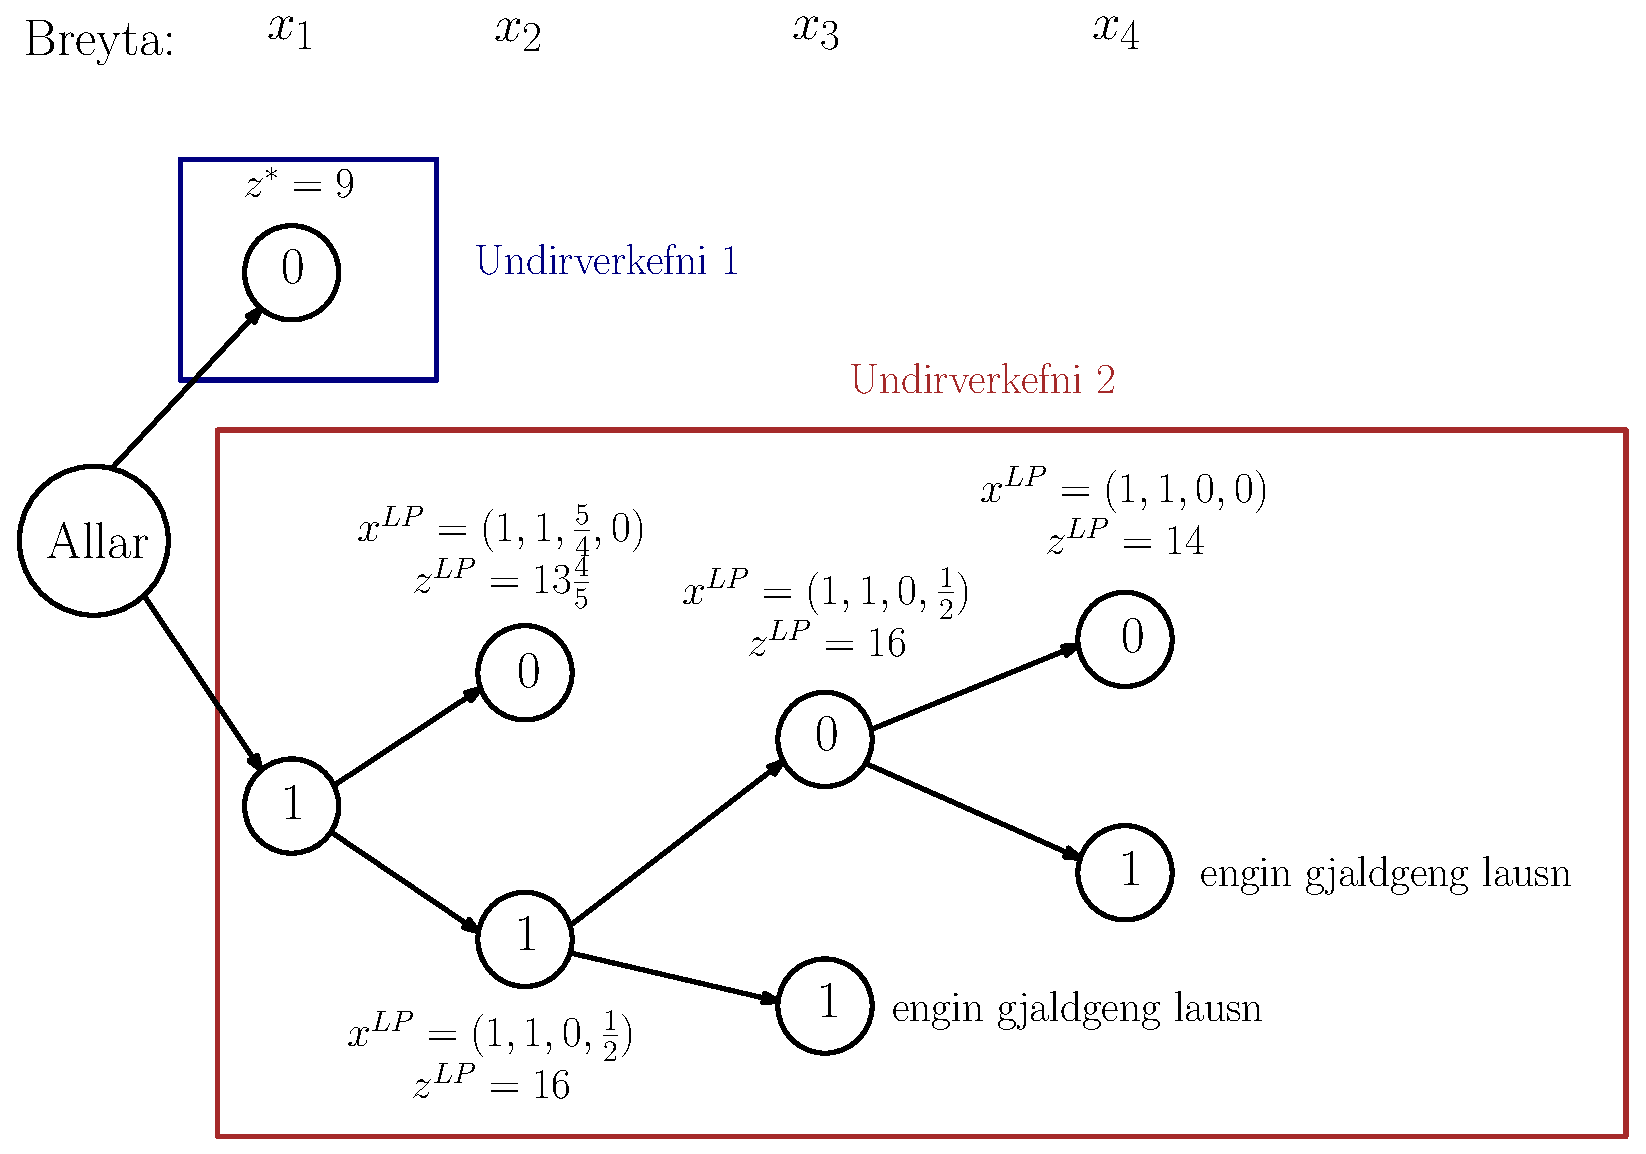
\includegraphics[width=0.9\columnwidth]{figs/branchandbound_full.eps}
\end{center}
\end{lausnSYND}

\begin{lausnSYND}[\emph{Branch-and-bound} með \textsc{glpk}] Þó svo \textsc{glpk} geti leyst tvíkostaverkefni, sbr. \texttt{var x, binary;} þá er minnsta mál að beita LP-tilslökun, og bæta við einni og einni skorðu fyrir hvert undirverkefni eins og gert var hér að ofan. Hér skiptir mestu máli að vera skipulagður í uppsetningu og kommenta réttar línur í hvert sinn forritið er keyrt.
\lstinputlisting{../glpk/branchandbound.mod}
  
\end{lausnSYND}


\subsection{\emph{Branch and bound} fyrir MIP}
\emph{Branch and bound} fyrir blönduð heiltöluverkefni.
\begin{daemi}
$$ \max_{\vec{x}} z = 4 x_1 - 2  x_2 + 7 x_3 - x_4$$
m.t.t. sk. 
\[\begin{array}{rrrrcl}
  x_1 &        &+~ 5 x_3 &        & \le & 10 \\
  x_1 &+~x_2   &-~   x_3 &        & \le & 1 \\
 6x_1 &-~ 5x_2 &         &        & \le & 0 \\
 -x_1 &        &+~  2x_3 & -~2x_4 & \le & 3
\end{array}\]
og
\begin{eqnarray*}
x_j \geq 0&& \mbox{ $j=1,2,3,4$. }\\
x_j && \mbox{ heiltala, $j=1,2,3$. }\\
x_4 &&  \mbox{ samfelld.}
\end{eqnarray*}
\end{daemi}



\begin{lausn}\hspace{.1cm}
  \begin{enumerate}[label=(\arabic{*})]\setcounter{enumi}{-1}
    \item Köllum fyrsta undirverkefnið $\mathcal{U}_0$. Setjum $z^*=-\infty$ (besta þekkta lausn á MIP hingað til).    
    Leysum línl. bestunarverkefnið með því að slaka á heiltölu kröfunni í $\mathcal{U}_0$.
 \begin{samepage}   \begin{aths} Annaðhvort í höndunum (Simplex-tafla) eða með \textsc{glpk}.     \end{aths}\end{samepage}
    Fáum LP-lausn: $\vec{x}=(1.25,1.5,1.75,0)$ með $z=14.25$.

    Sjáum að $x_1,x_2$ og $x_3$ eru ekki heiltölur, og þurfum því að kvísla verkefninu í frekari undirverkefni.

    Efra mark er $14.25$ -- við nálgum ekki því $x_4$ er \emph{ekki} heiltölubreyta.

    \item Veljum $x_1=1.25$ til að kvísla eftir:
    
    \begin{tabular}{p{7cm}|p{5cm}}
      $\mathcal{U}_0$ ásamt \mbox{$\mathcal{U}_1:~x_1\leq1$} &  $\mathcal{U}_0$ ásamt \mbox{$\mathcal{U}_2:~x_1\geq2$} \\
      \mbox{$\Rightarrow$ $\vec{x}=(1,1.2,1.8,0)$ með $z=14.2$}. &
      \mbox{$\Rightarrow$ engin gjaldgeng lausn}.
    \end{tabular}
    
    \item Getum eytt $\mathcal{U}_2$. Kvíslum $\mathcal{U}_1$ eftir $x_2=1.2$

    \begin{tabular}{p{6cm}|p{6cm}}
      $\mathcal{U}_0,\mathcal{U}_1$ ásamt \mbox{$\mathcal{U}_3:~x_2\leq1$} &
      $\mathcal{U}_0,\mathcal{U}_1$ ásamt \mbox{$\mathcal{U}_4:~x_2\leq2$} \\
      $\Rightarrow$ $\vec{x}=({\color{red}{0.833}},1,1.833,0)$ með $z=14.1667$. &
      $\Rightarrow$ $\vec{x}=({\color{red}{0.833}},2,1.833,0)$ með $z=12.1667$. 
    \end{tabular}

    \item Getum ekki eytt, en kvíslum frekar $\mathcal{U}_3$ því það hefur hærra efra mark. Bíðum með $\mathcal{U}_4$.
    Kvíslum $\mathcal{U}_3$  eftir $x_1=0.833$:

    \begin{tabular}{p{6cm}|p{6cm}}
      $\mathcal{U}_0,\mathcal{U}_1,\mathcal{U}_3$ ásamt \mbox{$\mathcal{U}_5:~x_1\leq0$} &
      $\mathcal{U}_0,\mathcal{U}_1,\mathcal{U}_3$ ásamt \mbox{$\mathcal{U}_6:~x_1\leq1$} \\
      $\Rightarrow$ engin gjaldgeng lausn &
      $\Rightarrow$ $\vec{x}=(0,0,2,0.5)$ með $z=13.5$. \\
      $\Rightarrow$ eyðum! &
      Fundum löglega lausn á $\mathcal{U}_0$, svo við uppfærum $z^*=13.5$. \\
      & $\Rightarrow$ eyðum! 
    \end{tabular}

    \item
    Getum núna eytt $\mathcal{U}_4$ því efra mark þess er $12.667<z^*$.
  
    \item Höfum afgreitt öll undirverkefni. Besta lausn er því $\vec{x}^*=(0,0,2,0.5)$ með $z^*=13.5$. 
  \end{enumerate}

\end{lausn}






\subsection{Samantekt á \emph{Branch and Bound} fyrir IP}

\begin{itemize}
\item Upphafsskref: Lát $Z=-\infty$. \begin{aths}Athugið \emph{fathoming test}, ef ekki er hægt að eyða verkefni, þá er þetta fyrsta undirverkefni.\end{aths}
\item \ath{Kvíslun} (e. branch): Af þeim undirvandamálum sem ekki hefur verið eytt, veljið það sem síðast var búið til, eða það sem hefur besta efra mark. Skiptið upp með því að setja gildi (0 eða 1) eða með því að setja bil $x_j\le[x_j^*]$ og $x_j\ge [x_j^*]+1$ ($x_j^*$ lausn á LP-tilslökunina).
 
% translate and add:
%  typical rules are the best bound rule which greedily uses the
%  remaining subset Ri with minimal value f0(Ri), and the newest
%  bound rule which partitions the most recently created subset.
%  A common method is to use the newest bound rule (depth first
%  tree search, so we find an incumbent quickly) but when there
%  is a choice of newly created sets, to use the best bound rule
%  to choose among them.
\item \ath{Efra mark} (e. bound ): Búið til efra mark með því að leysa aflappaða vandamálið með simplex aðferðinni.
\item \ath{Eyðing} (e. fathom ): Undirvandamáli er eytt ef:
\begin{itemize}
\item $F(1)$: eframark $\le z^*$,
\item $F(2)$: afslappaða verkefni þess hefur engar leyfilegar lausnir,
\item $F(3)$: afslappaða verkefni þess hefur heiltölulausn. Þessi er ný \emph{incumbent} lausn ef hún er betri.
\end{itemize}
\item Besta lausn fundin? Halda áfram uns engin undirvandamál eru eftir.  Síðasta \emph{incumbent} lausnin er besta lausn.
\end{itemize}

\begin{comment}
\begin{daemi}[MIP (sjá bls. 518 í bók)]
$$\max_{\vec{x}} Z = 4x_1 -2 x_2 + 7 x_3 - x_4$$
m.t.t. sk.
\begin{eqnarray*}
x_1 + 5 x_3  \le  10 \\
x_1 + x_2 - x_3  \le  1 \\
6 x_1 - 5 x_2  \le  0  \\
-x_1 + 2 x_3 - 2x_4  \le  3 \\
x_j\ge 0 \mbox{ og $j=1,2,3$ eru heiltölur.}
\end{eqnarray*}
\end{daemi}
\begin{lausn}\hspace{.1cm}
\lstinputlisting{matlab/branchandbound_script.m}
\end{lausn}
\end{comment}

\section{Kvíslisnið fyrir BIP verkefni}
\ath{Kvíslisnið} (e. branch-and-cut) fyrir tvíkostaverkefni, þ.e. ákvarðanabreytur eru annaðhvort 0 eða 1.

\emph{Hugmynd}: Forvinna BIP verkefnið þannig að það taki skemmri tíma til að leysa (án þess að útiloka gjaldgenga lausn). Aðferðir flokkast undir:

\begin{description}
\item[Festa ákvörðunarbreytur] annaðhvort sem $0$ eða $1$ þannig að besta lausnin sé ekki útilokuð, t.d. ef $3 x_1 \le 2$ þá er $x_1=0$.
\item[Eyða óþarfa skorðum] sem dæmi er skorðan $3x_1+2x_2 \le 6$ ofaukið, vegna þess að $3(1)+2(1) = 5  \le 6$. Getum eytt því skorðan verður alltaf uppfyllt.
\item[Þrengja skorður] minnka gjaldgengt svæði fyrir afslappað verkefni (LP-tilslökun) án þess að útiloka gjaldgengar lausnir á BIP verkefni. 
\end{description}

\subsection{Mynda kvíslisnið}
\begin{enumerate}
\item Athuga skorður sem eru aðeins með jákvæða stuðla og $\le$
  form, $$6x_1 + 3x_2+5x_3+2x_4 \le 10$$
\item Finna hóp af breytum (minnsta þekjugrúpa) þannig að:
\begin{itemize}
\item skorðan sé ekki gjaldgeng ef allar breytur í þekjugrúpu eru
  $1$ og allar aðrar breytur eru $0$, t.d. minnsta þekjugrúpa
  $\{x_1,x_3\}$, $$6(1)+3(0)+5(1)+2(0) = 11 \not\le 10$$
\item skorðan verður gjaldgeng ef ein breyta (eða fleiri) verður $0$
  í stað $1$, t.d.   $$6(1)+3(0)+5(\mathbf{0})+2(0) = 6 \le
  10$$ eða  $$6(\mathbf{0})+3(0)+5(1)+2(0) = 5 \le 10.$$
\item Lát $N$ vera fjölda breyta í minnstu þekjugrúpu $\mathcal{G}$, þá er
  hægt að mynda kvíslisnið á eftirfarandi formi:
$$\sum_{i\in\mathcal{G}}x_i \le N - 1$$
\end{itemize}
\end{enumerate}
\begin{daemi}Kvíslisnið fyrir $$6x_1 + 3x_2+5x_3+2x_4 \le 10$$\end{daemi}
\begin{lausn}
$$x_1 + x_3 \le 1$$
og
$$x_1+x_2+x_4\le 2$$
\end{lausn}
\subsection{Reiknirit til að þrengja skorður}
\lstinputlisting{../matlab/tighten.m}
\begin{daemi}$$\max_{\vec{x}} z = 3x_1 + 2 x_2$$
m.t.t. sk.
\begin{eqnarray*}
2x_1 + 3x_2  \le  4 \\
0\le x_1\le 1, 0\le x_2 \le 1
\end{eqnarray*}
\end{daemi}
\begin{lausn}Notum reikniritið hér að ofan:
\begin{lstlisting}
>> [a,b] = tighten([2 3], 4)

a =

     1     1

b =

     1
\end{lstlisting}
Skiptum því $2x_1 + 3x_2  \le  4$ út fyrir $x_1+x_2 \le 1$.

\begin{aths}Skorðan $x_1+x_2 \le 1$ hefur minnkað lausnarsvæði línulegu-tilslökunar umtalsvert, en sker ekki burt neinar gjaldgengar lausnir á tvíkostaverkefninu. Nú vill reyndar svo til að LP lausnin er $(0,1)$. 
\end{aths}

\end{lausn}

Þrenging á skorðum er dæmi um hvernig þrengja má lausnarsvæði LP-tilslökunar með því að útbúa \ath{skurðplön} (e. cutting plane). Sjá nánar bls. 514--515.


\chapter{Kvik bestun} 
Þegar taka þarf röð ákvarðana  yfir tímabil geta ákvarðanir sem teknar eru snemma í ferlinu haft áhrif á gæði þeirra sem síðar eru teknar. Ef skammtíma sjónarmið ráða eingöngu för, fæst niðurstaða sem yfirleitt er frábrugðin bestu mögulegu lausn. \ath{Kvika bestun} má oft nota bestu röð aðgerða.

\begin{description}
\item[\ath{Þrep}] (e. stages): hvert verkefni hefur $N$ þrep (tímaþrep) táknað með $n$ og á hverju þrepi er tekin ákvörðun $x_n$.
\item[\ath{Staða}] (e. state): á hverju þrepi $n$ eru nokkrar stöður $s_n$.
\item[\ath{Ákvörðun}] (e. action or policy decision): er byggð á $f_{n}^*(s_{n})$ þar sem $x^*_n$ er besta ákvörðunin á þrepi $n$ (lágmarka eða hámarka):
  $$f_n^*(s_n) = f_n(s_n,x_n^*) = \min_{x_n} f_n(s_n,x_n) \mbox{ eða } \max_{x_n} f_n(s_n,x_n)$$
\item[\ath{Besta stefna}] (e. optimal policy): markmið aðferðarinnar er að finna stefnu $\pi$ sem segir til um hvaða ákvörðun sé best $x^*_n = \pi^*(s_n)$ í hverju þrepi.
\item[\emph{$f_n(s_n,x_n)$}]  Tillegg til markfalls á þrepum $n,\ldots, N$ ef tekin er ákvörðun $x_n$ og síðan bestu ákvarðanir eftir það (á þrepum $n+1, \ldots, N$).
\item[\ath{Kostnaður}] $\mathcal{C}_{s_ns_{n+1}}^{x_n}$ er kostnaður við að taka ákvörðun $x_n$ og fara úr stöðu $s_n$ í stöðu $s_{n+1}$.
\item[\ath{Slembin kvik bestun}] (e. stochastic): $\mathcal{P}_{s_ns_{n+1}}^{x_n}$ er líkur á að fara úr stöðu $s_n$ í stöðu $s_{n+1}$ þegar ákvörðun $x_n$ er tekin. Í þessu   tilfelli er $f_n$ væntigildi (meðaltal).
\item[\ath{Óslembin kvik bestun}] (e. deterministic):
$$f_n^*(s_n) = \min_{x_n} \Big(\mathcal{C}_{s_ns_{n+1}}^{x_n}+ \alpha f_{n+1}^*(s_{n+1})\Big)$$
\item[\ath{Markov-eiginleiki}] gefið að við séum í stöðu $s_n$, þá er besta ákvörðun fyrir þau ástönd sem á eftir koma óháð því hvaða ákvarðanir voru teknar á fyrri þrepum   ($x_{n-1}, x_{n-2}, \ldots$).
\item[\ath{$N=\infty$}] þá stefnir $f_n\rightarrow\infty$, og því þarf $0 < \alpha <1$ (e. discount factor), annars notum við venjulega $\alpha=1$ þegar $N$ er takmarkað.
\item[\ath{Bellman-jafna}]
$$f_n^*(s_n) = \min_{x_n} \sum_{s_{n+1}\in
  s'}\mathcal{P}_{s_ns_{n+1}}^{x_n}\Big(\mathcal{C}_{s_ns_{n+1}}^{x_n}+ \alpha f_{n+1}^*(s_{n+1})\Big)$$
\end{description}
\begin{center}
\begin{figure}[h!]
  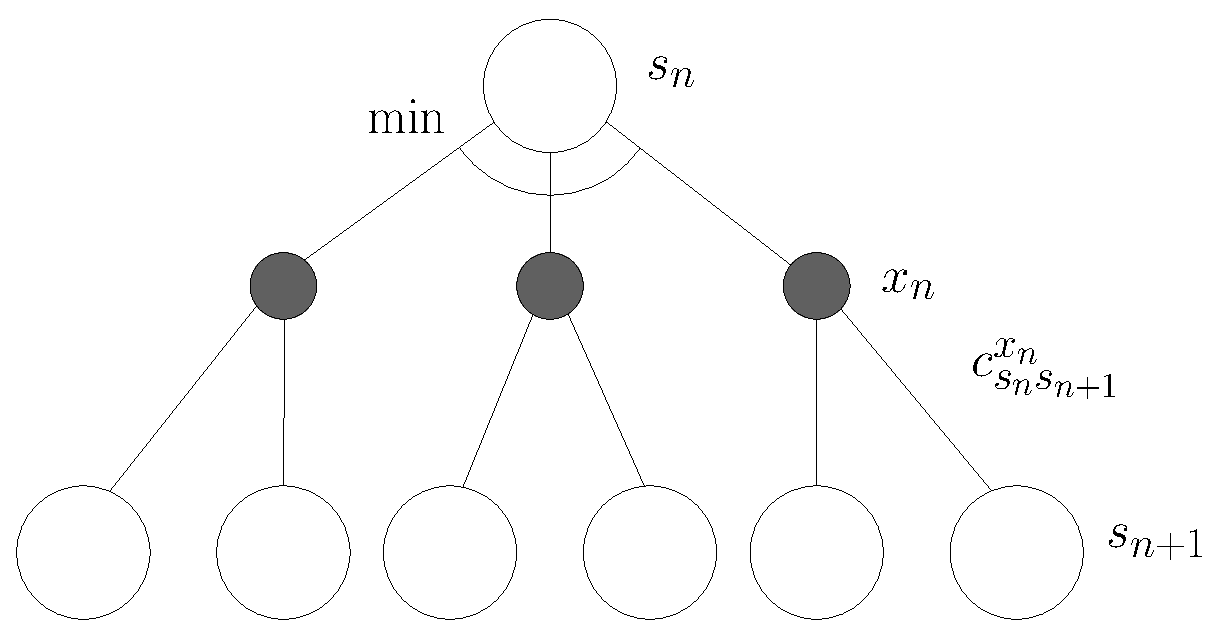
\includegraphics[width=0.9\columnwidth]{figs/stateaction.eps}
\end{figure}
\end{center}

\section{Aðferðin}
\begin{itemize}
\item Aðferð virkar með því að vinna sig afturábak frá  $n=N,N-1,\ldots,2,1$. 
\item Lesum bestu lausn áfram frá $n=1$.
\item Gefin besta ákvörðun í þrepi $n+1$ þá finnum við bestu ákvörðun í þrepi $n$ með því að nota \ath{endurkvæma sambandið} (e. recursive relationship), sem dæmi: 
$$f_n^*(s_n) = \min_{x_n} \Big(\mathcal{C}_{s_ns_{n+1}}^{x_n}+ f_{n+1}^*(s_{n+1})\Big)$$
\end{itemize}
\newpage
\begin{samepage}
\begin{aths}Afturvirka sambandið þarf ekki að vera línulegt,  annað dæmi um afturvirkt samband er 
$$f_n^*(s_n) = \min_{x_n} \Big(\mathcal{C}_{s_ns_{n+1}}^{x_n} f_{n+1}^*(s_{n+1})\Big)$$
 \end{aths}
\end{samepage}


Í kvikri bestun er oft \emph{unnið afturábak}. Oft er engan veginn augljóst hvernig leysa á bestunarverkefni með kvikri bestun -- listgrein frekar en vísindi. Best er að læra það m.þ.a. skoða (og leysa) nokkur dæmi.


\begin{daemi}[Leikur] Höfum eftirfarandi leikreglur:
  \begin{itemize}
    \item Tveir leikmenn
    \item 30 eldspýtur
    \item Leikmenn skiptast á að draga 1, 2 eða 3 eldspýtur
    \item Sá sem á leik þegar ein eldspýta er eftir tapar
  \end{itemize}
Hvernig getur sá sem byrjar tryggt sér sigur?
\end{daemi}
\begin{lausn}Setjum möguleg ástönd og aðgerðir upp í töflu.
\begin{center}
  \begin{tabular}{|cc|} \hline
    Fjöldi sem er eftir & Fjöldi eldspýta sem degnar eru \\
    (ástand) 		& (aðgerð) \\ \hline 
    \fbox{1}		&  tapar	\\ 
    2			&  1	\\ 
    3			&  2	\\ 
    4			&  3	\\ 
    \fbox{5}		&  tapar	\\ 
    6			&  1	\\ 
    7			&  2	\\ 
    8			&  3	\\  
    \fbox{9}		& tapar	\\ 
    $\vdots$		& \vdots	\\ \hline 
\end{tabular}
\end{center}
Ástönd sem leiða t.þ.a. andstæðingur tapar eru $T=\{1,5,9,13,17,21,25,29\}$.

Drögum eina eldspýtu í upphafi. Í framhaldinu er fjöldinn valinn þannig að andstæðingur lendi í einu af ástöndum $T$.
\end{lausn}

\begin{daemi}[Afbrigði af svonefndu \emph{bakpokaverkefni}]%\footnote{Sjá \href{http://en.wikipedia.org/wiki/Knapsack\_problem}{Knapsack problem}}]
Vörubíll getur í mesta lagi borið 10 tonna farm. Hægt er að senda þrjár mismunandi vörur með bílnum $V1,V2$ og $V3$. Þyngd og verðmæti eru:
\[ \begin{array}{|cl|ccc|} \hline
     & & V1 & V2 & V3 \\ \hline
    w & \mbox{þyngd (tonn)} & 1 & 2 & 2 \\
    u & \mbox{verðmæti} & 200 & 500 & 600 \\ \hline
   \end{array}\]
A.m.k. eitt stykki af hverri vöru á að fara í bílinn. 
Hvernig á að ferma bílinn þ.a. heildarverðmæti sé hámarkað?
\end{daemi}

\begin{lausn}\hspace{.1cm}

\begin{center}
\begin{tabular}{ll}
    Þrep & vara $i=1,2,3$. \\
    Ástand & $s_n=$ rými sem eftir er að ráðstafa á þrepi $n$\\
    Ákv.br.&  $x_n=$ magn sem sent er af vöru $i$ á þrepi $n$
\end{tabular}
\end{center}
\begin{aths}Þurfum að taka a.m.k. eitt stk. af hverri vöru $\Rightarrow$ 3 \emph{þrep} í verkefninu. Athugið einnig að þrepið er ekki tími, eins og oft er raunin í kvikri bestun).\end{aths}

Virði þess að taka ákvörðun $x_n$ á þrepi $n$ (og taka alltaf bestu ákvörðun eftir það) er gefið með eftirfarandi jöfnu:
$$ f_n(s_n)=x_n\cdot\underbrace{u_n}_{\tiny \mbox{verðmæti/ein}}+f^k_{n+1}(s_n-x_n\cdot\underbrace{w_n}_{\tiny \mbox{þyngd/ein}})$$

\begin{description}
  \item[Þrep $n=3$] Hér er um að ræða vöru 3, $w_3=2$ og $u_3=600$: Á þessu þrepi erum við búin að setja vörur 1 og 2 í bílinn og því mest $10-1-2=7$ tonn laus.
  \[\begin{array}{|c|c|c|}\hline 
    s_3 & f_3^*(s_3) & x_3^* \\ \hline 
    7	& 3\cdot600 & 3 \\
    6	& 3\cdot600 & 3 \\
    5	& 2\cdot600 & 2 \\
    4	& 2\cdot600 & 2 \\
    3	& 1\cdot600 & 1 \\
    2	& 1\cdot600 & 1 \\    \hline
    \end{array}\]
  \item[Þrep $n=2$] Hér er um að ræða vöru 2, $w_2=2$ og $u_2=500$: Á þessu þrepi erum við búin að setja vöru 1 í bílinn og því mest $10-1=9$ tonn laus.
  \[\begin{array}{|c|ccc|c|c|}\hline 
    s_2\backslash x_2 & \multicolumn{3}{c|}{f_2(s_2,x_2)=x_2u_2+f^*_3(s_2-x_2w_2)} &f_2^*(s_2)&  x_2^* \\ 
	& x_2=1	&	x_2=2	&	x_2=3	&	&	\\\hline 
    9	& 1\cdot500+1800 	& 2\cdot500+1200 	& 3\cdot600 	&2300	&	1\\
    8	& 1\cdot500+1800 	& 2\cdot500+1200 	& 3\cdot600 	&2300	&	1\\    
    7	& 1\cdot500+1200 	& 2\cdot500+600 	& - 		&1700	&	1\\
    6	& 1\cdot500+1200 	& 2\cdot500+600 	& -		&1700	&	1\\
    5	& 1\cdot500+600 	& - 			& - 		&1100	&	1\\
    4	& 1\cdot500+600 	& -			& - 		&1100	&	1\\
    \hline
    \end{array}\]
  \item[Þrep $n=1$] Hér er um að ræða vöru 1, $w_1=1$ og $u_1=200$: Á þessu þrepi er bílinn tómur og því 10 tonn til umráðanna
  \[\begin{array}{|c|cccccc|c|c|}\hline 
    s_1\backslash x_1 & \multicolumn{6}{c|}{f_1(s_1,x_1)=x_1u_1+f^*_2(s_1-x_1w_1)} &f_1^*(s_1)&  x_1^* \\ 
	& 1 & 2 & 3&4&5&6&&	\\\hline 
    10	& 1\cdot200	&2\cdot200	&3\cdot200&4\cdot200&5\cdot200&6\cdot200& 2700	&	2\\
    	& +2300 	&+2300		&+1700&+1700&+1100&+1100& &	\\
    \hline
    \end{array}\]
\end{description}
Sjáum strax hvað besta gildi markfalls er, nefnilega $z^*=f_1^*(s_1)=2700$. Til að finna bestu lausnina, þá þurfum við að lesa hana afturábak: $$x_1^*=2 \stackrel{s_2=8}{\longrightarrow} x_2^*=1\stackrel{s_3=6}{\longrightarrow} x_3^*=3.$$
\end{lausn}

\begin{comment}
Í kvikri bestun eru teknar ákvarðanir (e. decision) á \ath{þrepum} (e. stage) verkefnisins. Á sérhverju þrepi koma eitt eða fleiri \ath{ástönd} (e. stage) til greina. Ákvörðun í einhverju ástandi á tilteknu ástandi leiðir til \ath{færslu} (e. transition) yfir í ástand á næsta þrepi.

Svarandi til sérhvers (þrep,ástand) er \ath{virðisfall} (e. value function) sem er besta gildi á markfalli sem hægt er að ná m.þ.a. byrja í viðkomandi ástandi (og hegða sér optimalt eftir það).

\ath{Endurkvæmt samband} (e. recursive relation) ríkir milli virðisfalla fyrir mismunandi ástönd.

Safn ákvarðana fyrir öll  mögulega ástönd mynda \ath{stefnureglu} (e. policy) ákvarðanatakans. Erum að leita að bestu stefnureglu í tilteknu verkefni. 

Látum 
\begin{enumerate}
  \item[$N$] fjöldi þrepa
  \item[$n$] núverandi þrep ($n\in\{1,..,N\}$
  \item[$s_n$] ástand á þrepi $n$
  \item[$x_n$] ákvörðun á þrepi $n$
  \item[$x_n^*$] besta gildi $x_n$ (gefið $s_n$)
  \item[$f_n(s_n,x_n)$] framlag þrepa $n,n+1,..,N$ til markfallsins m.v. að byrjað sé í ástandi $s_n$ á þrepi $n$, ákvörðun $x_n$ sé þekkt og bestu ákvarðanir séu teknar þar á eftir.
  \item[$f_n^*(s_n,x_n)$] $=\max_{x_n} f_n(s_n,x_n)$ (eða $\min$)
\end{enumerate}

\begin{center}
  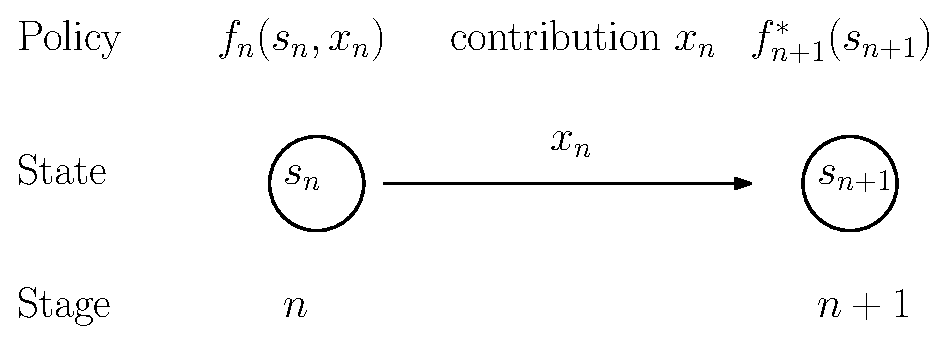
\includegraphics[width=0.5\columnwidth]{figs/stagestep.eps}
\end{center}
\end{comment}

\begin{daemi}[Skipan rannsóknateyma]Höfum gefnar forsendur:
  \begin{itemize}
    \item Þrjú teymi glíma við sama verkefnið (geimferðaáætlun) en nota mismunandi aðferðir
    \item Líkur á að hópunum \emph{mistakist} að leysa verkefnið hefur verið metnar eftirfarandi:
    \[\begin{matrix}       1 & 0.4 \\ 2 & 0.6 \\ 3 & 0.8       \end{matrix}\]
    Líkur að öllum mistekist er því $0.4\cdot0.6\cdot0.8=0.192$.
  \end{itemize}
  Nú bætast við tveir toppmenn við í verkefnið. Hvernig á að ráðstafa þessum nýju mönnum þ.a. líkur á að öllum hópum mistakist séu lágmarkaðar m.v. að líkur á að mistakast séu eftirfarandi:
 \[\begin{array}{|c|ccc|} \hline \mbox{fj. sem } & \multicolumn{3}{c|}{\mbox{Hópur}}\\
  \mbox{bætist við}& 1 & 2 & 3 \\ \hline
  0 & 0.4 & 0.6 & 0.8 \\
  1 & 0.2 & 0.4 & 0.5 \\
  2 & 0.15 & 0.2 & 0.3    \\\hline   
   \end{array}\]
\end{daemi}
\begin{lausn}Látum
%Er raunhæft að finna bestu lausn m.þ.a. prófa einfaldlega alla möguleika?  
\begin{center}\begin{tabular}{lp{7cm}}
  Þrep $n$ & teymi $1,2,3$ \\
  Ástand $s_n$ &  fjöldi sem \emph{eftir} er að ráðstafa á þrepin \\
  Ákv.br. $x_n$ & fjöldi sem úthlutað er á hóp $n$ \\
  $p_i(x_i)$ & líkur á að teymi $i$ mistakist m.v. að $x_i$ mönnum hafi verið bætt við hóp $i$.
\end{tabular}\end{center}
Líkur á að öllum mistakist eru $p(x_1)p(x_2)p(x_3)$. Lágmörkum þá stærð, þ.e.
  $$ \min_{\vec{x}} p(x_1)p(x_2)p(x_3)$$
m.t.t. sk. $$x_1+x_2+x_3=2$$ $$x_i\geq0,~~x_i\mbox{ heiltölur}$$
Þá er 
$$f_n(s_n,x_n)=p_n(x_n)f^*_{n+1}(s_n-x_n)$$
með
$$f_n^*(s_n,x_n)=\min_{x_n\in\{0,..,s_n\}}f_n(s_n,x_n)$$
  
\begin{description}
  \item[Þrep $n=3$]
{\scriptsize
  \[\begin{array}{|c|c|c|}\hline 
    s_3 & f_3^*(s_3) & x_3^* \\ \hline 
    0	& 0.8 & 0 \\
    1	& 0.5 & 1 \\
    2	& 0.3 & 2 \\    \hline
    \end{array}\]}
  \item[Þrep $n=2$]
{\scriptsize
  \[\begin{array}{|c|ccc|c|c|}\hline 
    s_2\backslash x_2 & \multicolumn{3}{c|}{f_2(s_2,x_2)=p_2(x_2)f^*_3(s_2-x_2)} &f_2^*(s_2)&  x_2^* \\ 
	& x_2=0	&	x_2=1	&	x_2=2	&	&	\\\hline 
    0	& 0.6\cdot0.8=0.48 	& - 	& - & 0.48&	0\\
    1	& 0.6\cdot0.5=0.30 	& 0.4\cdot0.8=0.32 	& - &0.3&	0\\    
    2	& 0.6\cdot0.3=0.18 	& 0.4\cdot0.5=0.2 	& 0.2\cdot0.8=0.16	&0.16&	2\\
    \hline
    \end{array}\]}
  \item[Þrep $n=1$]
{\scriptsize 
  \[\begin{array}{|c|ccc|c|c|}\hline 
    s_1\backslash x_1 & \multicolumn{3}{c|}{f_1(s_1,x_1)=p_1(x_1)f^*_2(s_1-x_1)} &f_1^*(s_1)&  x_1^* \\ 
	& x_1=0	&	x_1=1	&	x_1=2	&	&	\\\hline 
    2	& 0.4\cdot0.16=0.064 	& 0.2\cdot0.3=0.06 	& 0.15\cdot0.48=0.072	&0.06&	1\\
    \hline
    \end{array}\]}
\end{description}
Besta lausn er $$x_1^*=1\stackrel{s_2=1}{\longrightarrow}x_2^*=0\stackrel{s_3=1}{\longrightarrow}x_3^*=1$$ sem gefur líkurnar að öllum mistekist eru 0.06.

\end{lausn}
\begin{daemi}[Lagerhald]
  Fyrirtæki framleiðir eina tegund vöru og selur áfram.
  \begin{center}\begin{tabular}{ll}
    $d_j$ & Eftirspurn í mánuði $j$ (gefin) \\
    $x_j$ & Magn sem á að framleiða (ákv.breyta) \\
    $i_j$ & Lagerstaða í upphafi $j$-ta tímabils (ástand)
  \end{tabular}\end{center}
Í mánuði $i$ gildir
$$i_{j+1}=i_j+x_j-d_j$$
G.r.f. að $i_1$ sé þekkt (upphafsstaða) og lager verði tómur í lokin. Að auki er g.r.f. að $d_j,i_j$ og $x_j$ séu heiltölur.

Kostnaður vegna framleiðslu í mánuði $j$ er
$$ \mathcal{C}_j(x_j)=\Bigg\{\begin{array}{cl} 0 & \mbox{ef } x_j=0\\ K_j+c_j(x_j) & \mbox{ef } x_j\geq0\end{array}$$
þar sem $K_j$ er uppsetningarkostnaður í mánuði $j$ og $c_j$ er einhver kostnaður háður  magni.

Þessu til viðbótar er birgðahaldskostnaður $h_j$ á einingu í mán. $j$. 
Hver eru þrep, ástönd, ákvarðanabreytur og virðisfall verkefnisins?
\end{daemi}
\begin{lausn}\hspace{.1cm}

\begin{center}  \begin{tabular}{lp{10cm}}
    Þrep &  tímabil $n\in\{1,2,..,N\}$ \\
    Ástand & lagerstaða í lok tímabils $j$, þ.e. $i_{j+1}$ \\
    Ákv.br. & $x_j$ er hversu mikið á að framleiða í mán. $j$ \\
    Virðisfallið & er heildarkostnaður: $ f(x_j,i_{j+1})=\mathcal{C}_j(x_j)+h_ji_{j+1}.$
  \end{tabular}\end{center}
\end{lausn}

\begin{daemi}[Birgðastýring]
  \[\begin{array}{|cccc|}\hline
    \mbox{Tímabil} & \mbox{Eftirspurn} (d_j) & \mbox{Upps.kostn} (K_j) & \mbox{Lagerk.} (h_j) \\\hline
1 & 3 & 3 & 1 \\
2 & 2 & 7 & 3 \\
3 & 4 & 6 & 2 \\ \hline
  \end{array}\]
Breytilegur kostnaður er $c_j=10$ fyrir fyrstu 3 einingarnar og 20 fyrir þær sem eru umfram það. Í upphafi er $i_1=1$.
\end{daemi}
\newpage
\begin{lausnSYND}\hspace{.1cm}
\begin{description}
  \item[Þrep $n=1$] Hér er $d_1=3$ en við höfum $i_1=1$, því framleiðum við minnst $x_1=d_1-i_1=2$ og til að dekka alla mögulegar framtíðar eftirspurnir þá þarf $x_1\leq d_2+d_3=2+4$. Því skoðum við $x_1\in\{2,..,6\}$.

Þurfum á $\mathcal{C}_1(x_1)$ að halda í töflunni:
\[ \begin{array}{cccccccc} x_1 & 2 &3&4&5&6&7&8\\\hline\mathcal{C}_1(x_1)&23&33&53&73&93&113&133\end{array}\]
{\scriptsize
\[\begin{array}{|cc|ccccccc|c|c|}\hline
  i_2 & h_1i_2 & \multicolumn{7}{c|}{f_1^*(i_2)=\mathcal{C}_1(x_1)+h_1i_2} & f^*(i_2) & x_1^* \\
\mbox{ástand} & \mbox{kostn} & 2 & 3 & 4 & 5 & 6 & 7 &8 &&\\ \hline 
0 & 0 & 23 &&&&&&& 23 & 2 \\
1 & 1 && 34 &&&&&& 34 & 3 \\
2 & 2 &&& 55 &&&&& 55 & 4 \\
3 & 3 &&&& 76 &&&& 76 & 5 \\
4 & 4 &&&&& 97 &&& 97 & 6 \\
5 & 5 &&&&&&118 && 118& 7 \\
6 & 6 &&&&&&& 139 & 139& 8 \\
\hline \end{array}\]}
\item[Þrep $n=2$]
\[ \begin{array}{cccccccc} x_2 & 0&1&2 &3&4&5&6\\\hline\mathcal{C}_2(x_2)&0&17&27&37&57&77&97\end{array}\]
{\scriptsize
\[\begin{array}{|cc|ccccccc|c|c|}\hline
  i_3 & h_2i_3 & \multicolumn{7}{c|}{f_2^*(i_3)=\mathcal{C}_2(x_2)+h_2i_3+f_1^*(i_3+d_2-x_2)} & f^*(i_3) & x_2^* \\
 &  & 2 & 3 & 4 & 5 & 6 & 7 &8 &&\\ \hline 
0 & 0 & 0+55 &17+34&27+23&-&-&-&-& 50 & 2 \\
1 & 3 &3+76& 20+55 &30+34&40+23&-&-&-& 63 & 3 \\
2 & 6 &6+97&23+76&33+55 &43+34&63+23&-&-& 77 & 3 \\
3 & 9 &9+118&26+97&36+76&46+55&66+34&86+23&-& 100 & 4 \\
4 & 12 &12+139&29+118&39+97&49+76&69+55&89+34&109+23& 123 & 5 \\
\hline \end{array}\]}
\item[Þrep $n=3$]
\[ \begin{array}{cccccc} x_3 & 0&1&2 &3&4\\\hline\mathcal{C}_3(x_3)&0&16&26&36&56\end{array}\]
{\scriptsize
\[\begin{array}{|cc|ccccc|c|c|}\hline
  i_4 & h_3i_4 & \multicolumn{5}{c|}{f_3^*(i_4)=\mathcal{C}_3(x_3)+h_3i_4+f_2^*(i_4+d_3-x_3)} & f^*(i_4) & x_3^* \\
 &  &0&1& 2 & 3 & 4 & &\\ \hline 
0 & 0 & 0+123&16+100&26+77&36+63&56+50&99&3\\
\hline \end{array}\]}
\end{description}
Besta lausn fæst m.þ.a. rekja sig afturábak:
$$\stackrel{i_4=0}{\longrightarrow}\fbox{$x_3^*=3$}\stackrel{i_3=i_4+d_3-x_3=1}{\longrightarrow}\fbox{$x_2^*=1$}\stackrel{i_2=i_3+d_2-x_2=0}{\longrightarrow}\fbox{$x_1^*=2$}$$ með heildarkostnað $z^*=99$.
\end{lausnSYND}


\section*{Mismunandi snið}
\[
\begin{array}{ll}
  \mathcal{C}_{s_n}(x_n)+f^*_{n+1}(s_{n+1}) & \min \sum_{n=1}^N \mathcal{C}_{s_n}(x_n) \\
  p_n(x_n)+f^*_{n+1}(s_n-x_n) & \max \sum_{n=1}^N p_n(x_n) \\
  p_n(x_n)\cdot f^*_{n+1}(s_n-x_n) & \max \prod_{n=1}^N p_n(x_n) \\
  x_nu_n+f^*_{n+1}(s_n-x_nw_n) & \max \sum_{n=1}^N x_nu_n \\
\end{array}
\]



\begin{comment}
\begin{daemi}[Spilavíti]
\begin{itemize}
\item Spilum $3$ leiki, $n=1,2,3$ (þrep).
\item Veðjum $x_n$ spilapeninga (ákvörðun).
\item Fjöldi spilapeninga er $s_n$ (staða).
\item Viljum hámarka líkur á að vera með $5$ peninga í lokin  (markmið).
\item Hvernig á að veðja? (besta stefna).
\item Gefið: P( vinnum $x$) $= \frac{2}{3}$, P( töpum $x$) $=\frac{1}{3}$.
\end{itemize}
Bellman jafna:
$$f_n^*(s_n) = \max_{x_n} \sum_{s_{n+1}\in
  s'}\mathcal{P}_{s_ns_{n+1}}^{x_n}\Big(\mathcal{C}_{s_ns_{n+1}}^{x_n}+ \alpha f_{n+1}^*(s_{n+1})\Big)$$
\end{daemi}
\begin{lausn}
 \begin{eqnarray*}
f_n(s_n) &=& \sum_{s_{n+1}\in  s'}\mathcal{P}_{s_ns_{n+1}}^{x_n} f_{n+1}^*(s_{n+1})\\
& =& \frac{1}{3}f_{n+1}^*(s_n-x_n)+\frac{2}{3}f_{n+1}^*(s_n+x_n)
\end{eqnarray*}
þar sem $f_4^*(s_4) = 0$ (terminal state) ef $s_4<5$ og $1$ ef $s_4\ge 5$.
Ritháttur: 
\begin{eqnarray*}
 x_n \textrm{ tapar}: & s_{n+1}=s_n-x_n \\
 x_n \textrm{ vinnur}: & s_{n+1}=s_n+x_n
\end{eqnarray*}
\vspace{5cm}
\begin{center}
  \includegraphics[width=0.9\columnwidth]{figs/spilaviti1.eps}
  \includegraphics[width=0.9\columnwidth]{figs/spilaviti2.eps}
\end{center}
\end{lausn}


\begin{daemi}[Úthlutun á heilsugæsluteymum til vanþróaðra landa]Höfum fimm teymi sem úthluta þarf til þriggja landa. 

Hvernig á að úthluta teymunum til að hámarka jákvæð áhrif teymanna á heilsu landsmanna?

Aukning í fjölda mannára ef teymum er úthlutað á viðkomandi land:

\centering
\begin{tabular}{l|l|l|l}
\hline
Fjöldi teyma & land 1 & land 2 & land 3\\
\hline
0 & 0 & 0 & 0 \\
1 & 45 & 20 & 50 \\
2 & 70 & 45 & 70 \\
3 & 90 & 75 & 80 \\
4 & 105 & 110 & 100 \\
5 & 120 & 150 & 130 \\
\hline
\end{tabular}
\begin{center}
  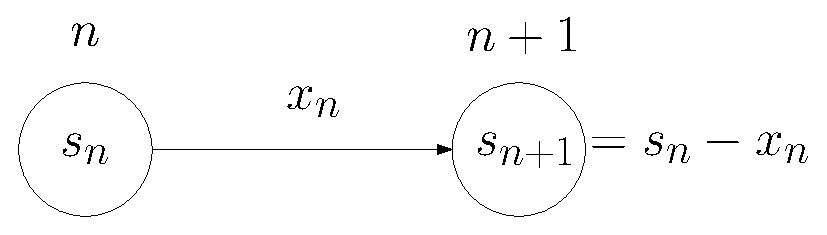
\includegraphics[width=0.5\columnwidth]{figs/teymi.eps}
\end{center}

\end{daemi}
\begin{lausn}
\begin{itemize}
\item {\bf Staða}: magn aðfanga til ráðstöfunar
\item $x_n$: magn aðfanga sem úthlutað er á þrepi $n$.
\end{itemize}Viljum leysa
$$\max_{x_1,x_2,x_3} ~~~ \sum_{i=1}^3 \mbox{jákvæð áhrif}
(x_i)$$
m.t.t. sk $$\sum_{i=1}^3 x_i = 5, \quad x_i \textrm{ eru jákvæðar heiltölur}.$$
\begin{center}
  \includegraphics[width=0.5\columnwidth,angle=-2]{figs/teymi1.eps}
  \includegraphics[width=0.9\columnwidth,angle=1]{figs/teymi2.eps}
  \includegraphics[width=0.9\columnwidth,angle=-2]{figs/teymi3.eps}
  \includegraphics[width=\columnwidth,angle=-2]{figs/teymi4.eps}
\end{center}
\end{lausn}
\end{comment}
\chapter{Þumalputtareglur}
Fram að þessu höfum við skoðað aðferðir sem finna bestu lausn á há- eða lágmörkunarverkefnum sbr. Simplex-aðferðin fyrir línulega bestun og \emph{branch and bound} fyrir heiltölubestun.

Mörg hagnýt verkefni í aðgerðagreiningu eru af þeirri stærðargráðu að illmögulegt eða jafnvel ómögulegt er að finna bestu lausn.

Í slíkum tilfellum er ásættanlegt að finna \emph{góða} lausn, þ.e. gjaldgenga lausn sem er ekki mikið verri en sú besta.

Svonefndar \ath{brjóstvitsaðferðir} (e. heuristics) eru oft notaðar til að finna slíkar nálgunarlausnir.

Eitt þekktasta dæmið snýst um farandsölumann (e. Travelling Salesman Problem -- TSP) sem ætlar að heimsækja nokkra bæi. Verkefnið felst í því að heimsækja sérhvern bæ einu sinni áður en hann snýr til baka í bæinn sem hann býr í, þannig að heildarvegalengd sé sem minnst.

\begin{daemi}[TSP]\label{daemi:tsp}\hspace{.1cm}
\begin{center}
  \includegraphics[width=0.6\columnwidth]{figs/tsp.eps}
\end{center}
\end{daemi}

Skyld verkefni eru m.a.
\begin{itemize}
  \item Vöruútkeyrsla
  \item Framleiðsla á prentplötum
\end{itemize}

\begin{aths}Fjöldi mögulegra leiða ef fjöldi bæja er $n$ er:
$$ \frac{(n-1)(n-2)\cdots(1)}{2}=\frac{(n-1)!}{2}$$
Þannig að fyrir $n=20$ eru þetta $10^{16}$ gjaldgengar leiðir, en fyrir $n=50$ eru þetta $10^{62}$ gjaldgengar leiðir!  
\end{aths}

Framgangsmáti nálgunaraðferða er yfirleitt þannig að fyrst er fundin einhver gjaldgeng lausn (getur verið mjög erfitt) og síðan eru smávægilegar bætingar á lausninni gerðar ítrekað.

Dæmi um slíkar endurbætur í verkefni farandsölumannsins er að víxla á tveimur eða fleiri áfangastöðum (e. subtour reversal).

\begin{lausnSYND}[á TSP dæmi \ref{daemi:tsp}]Höfum gefna upphafslausn þar sem farandsölumaðurinn fer $1\to2\to3\to4\to5\to6\to7\to1$ með fjarlægð 69.
\begin{center}
  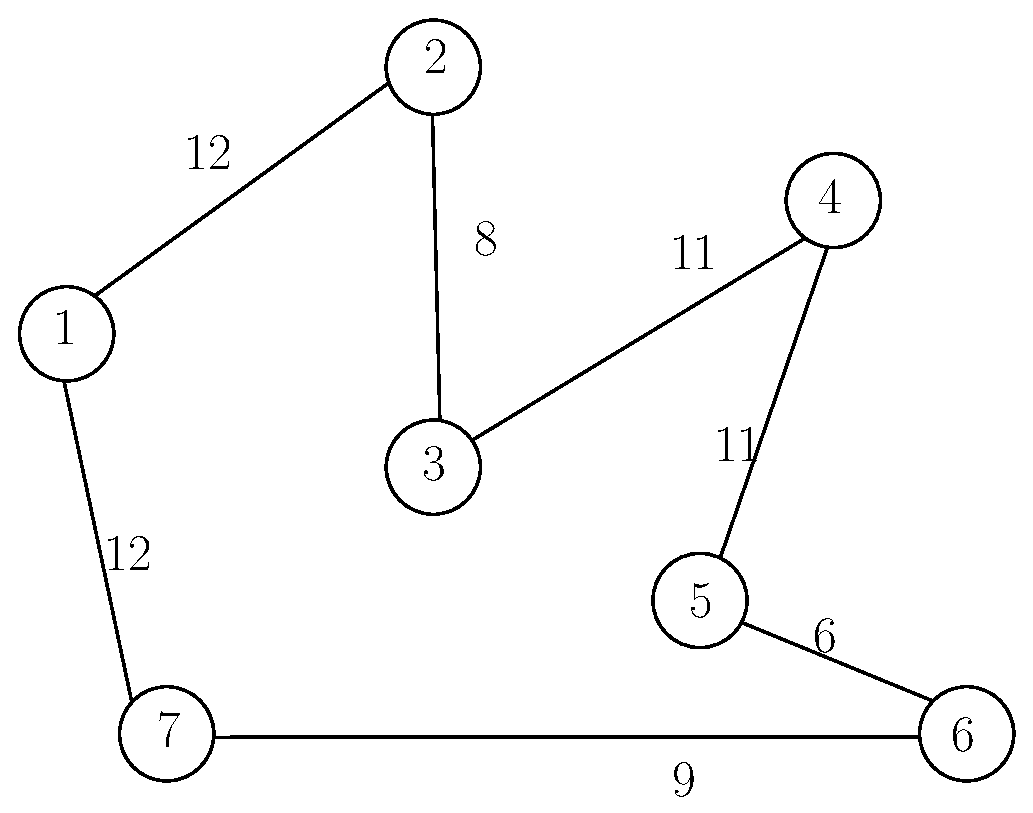
\includegraphics[width=0.6\columnwidth]{figs/tsp_12345671.eps}
\end{center}
Prófum að víxla á $2\to3,3\to4,4\to5$ og $5\to6$. 
\newpage
Ef víxlað er t.d. á $3\to4$ verður vegalengdin 65 -- sem er stytting um 4.
\begin{center}
  \includegraphics[width=0.5\columnwidth]{figs/tsp_12435671.eps}
\end{center}

Á sama  hátt fæst
\begin{center}
  \begin{tabular}{|c|c|c|ll}\cline{1-3}
    Víxlað & Leið & Vegalengd \\ \cline{1-3}
        & $1-2-3-4-5-6-7-1$ & 69 \\
$2\to3$ & $1-3-2-4-5-6-7-1$ & 68 \\
$3\to4$ & $1-2-4-3-5-6-7-1$ & \fbox{65} & $\nwarrow$\multirow{2}{*}{Mesta bæting}\\
$4\to5$ & $1-2-3-5-4-6-7-1$ & \fbox{65} & $\swarrow$\\
$5\to6$ & $1-2-3-4-6-5-7-1$ & 66 \\ \cline{1-3}
  \end{tabular}
\end{center}
Veljum t.d. $1-2-4-3-5-6-7-1$ (sjá mynd hér að ofan). Hægt er að stytta enn frekar m.þ.a. víxla $3-5-6$, og fá vegalend 64.
\begin{center}
  \includegraphics[width=0.5\columnwidth]{figs/tsp_12465371.eps}
\end{center}
Ekki er hægt að stytta vegalend meira með þessari aðferð. Hún finnur því \emph{ekki} bestu lausn, $1-2-4-6-7-5-3-1$  með vegalengd 63.

Við segjum að aðferðin sé föst í \emph{staðbundnu lággildi} (e. local optimum).

  
\end{lausnSYND}

\begin{samepage}
\begin{lausn}[Heiltöluframsetning á TSP \ref{daemi:tsp}]
Gefið:
\begin{enumerate}
  \item[$\mathcal{V}$] mengi hnúta,
  \item[$\mathcal{E}$] mengi leggja $\mathcal{E}\subset \mathcal{V}\times\mathcal{V}$,
  \item[$c_{ij}$] vegalengd frá $i$ til $j$,
  \item[$n$] fjöldi hnúta, $n=|\mathcal{V}|$.
\end{enumerate}
Ákvarðanabreytur:
\[ x_{ij}=\Bigg\{\begin{array}{cl}1 & \textrm{ef sölumaður fer úr bæ $i$ til bæ $j$} \\ 0 & \textrm{annars}\end{array}\]
Markfall 
\[ \min_{\vec{x}} \sum_{(i,j)\in\mathcal{E}}c_{ij}x_{ij}\]
m.t.t. skorða
\begin{eqnarray*}
  \sum_{j:\;(i,j)\in\mathcal{E}}x_{ij}=1 &\quad \forall i\in\mathcal{V}\quad & \mbox{yfirgefur bæ $i$ einu sinni}\\
  \sum_{i:\;(i,j)\in\mathcal{E}}x_{ij}=1 &\quad \forall j\in\mathcal{V}\quad & \mbox{förum einu sinni í bæ }j\\
\end{eqnarray*}

  \begin{aths}
    Þessar skorður duga ekki til -- því við getum fengið ósamanhangandi lausnir.
  \end{aths}

Margar leiðir eru þekktar t.þ.a. tryggja það að lokalausn sé samanhangandi. Ein slík er að láta sölumanninn selja nákvæmlega einn hlut í hverjum bæ. Bætum við ákvarðanabreytu:
\begin{enumerate}
  \item[$y_{ij}$] Fjöldi hluta sem sölumaður á eftir að hafa yfirgefið bæ $i$ og áður en hann kemur í bæ $j$ (flæði um legg $(i,j)$), $y_{ij}\geq0$. 
\end{enumerate}
og skorðum
\[y_{ij} \leq (n-1)x_{ij} \quad\quad\forall(i,j)\in\mathcal{E} \]
\begin{eqnarray*}
  \sum_{j:\;(j,i)\in\mathcal{E}}y_{ji}&=&\sum_{j:\;(i,j)\in\mathcal{E}}y_{ij}+1\quad\forall i\in\mathcal{V}\backslash\{i\} \\
  \sum_{j:\;(j,i)\in\mathcal{E}}y_{ji}+n&=&\sum_{j:\;(i,j)\in\mathcal{E}}y_{ij}+1\quad i=1 
\end{eqnarray*}
\begin{aths}Getum notað \textsc{glpk} t.þ.a. leysa TSP með 16--20 bæjum.\end{aths}
\end{lausn}
\end{samepage}

Bestunarverkefni sem hafa fleiri en eitt \ath{staðbundið lággildi} (e. local optimum) eru sögð vera \ath{víðvær} (e. global).


\begin{daemi}
  Hámarka $f(x)=12x^5-975x^4+28000x^3-345000x^2+1800000x$ með $0\leq x\leq 31$. 
\end{daemi}
\begin{lausnSYND}
Rissum upp feril fallsins og finnum þannig hágildispunktinn.
\begin{center}
  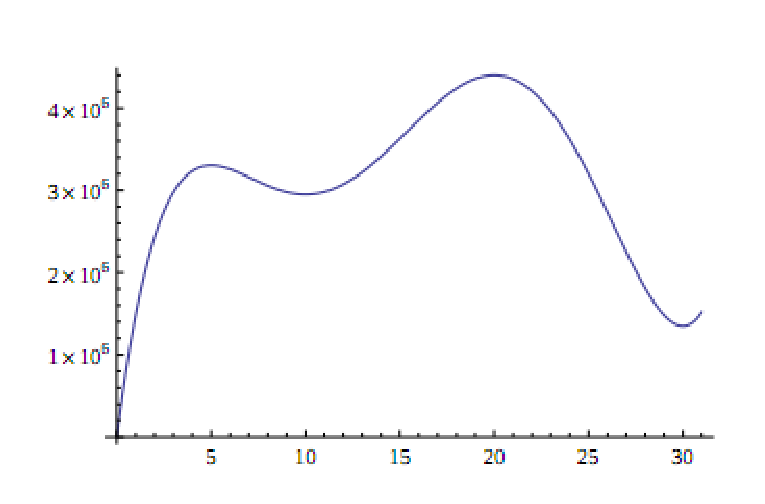
\includegraphics[width=0.5\columnwidth]{figs/global_opt.eps}
\end{center}
\end{lausnSYND}


\begin{daemi}
  Hámarka $f(x)=\cos(x_1)^2+\sin(x_2)^2$ með $-5\leq x_1\leq 5$, $-5\leq x_2\leq 5$. 
\end{daemi}
\begin{lausnSYND}
  Rissum feril fallsins með \textsc{Matlab} á eftirfarandi hátt:
\begin{lstlisting}[language=matlab]
>> [x1,x2]=meshgrid(-5:0.1:5,-5:0.1:5);
>> f=cos(x1).^2+sin(x2).^2;
>> surf(x1,x2,f);
>> shading interp
>> xlabel('x1'), ylabel('x2')
\end{lstlisting}
\begin{center}
  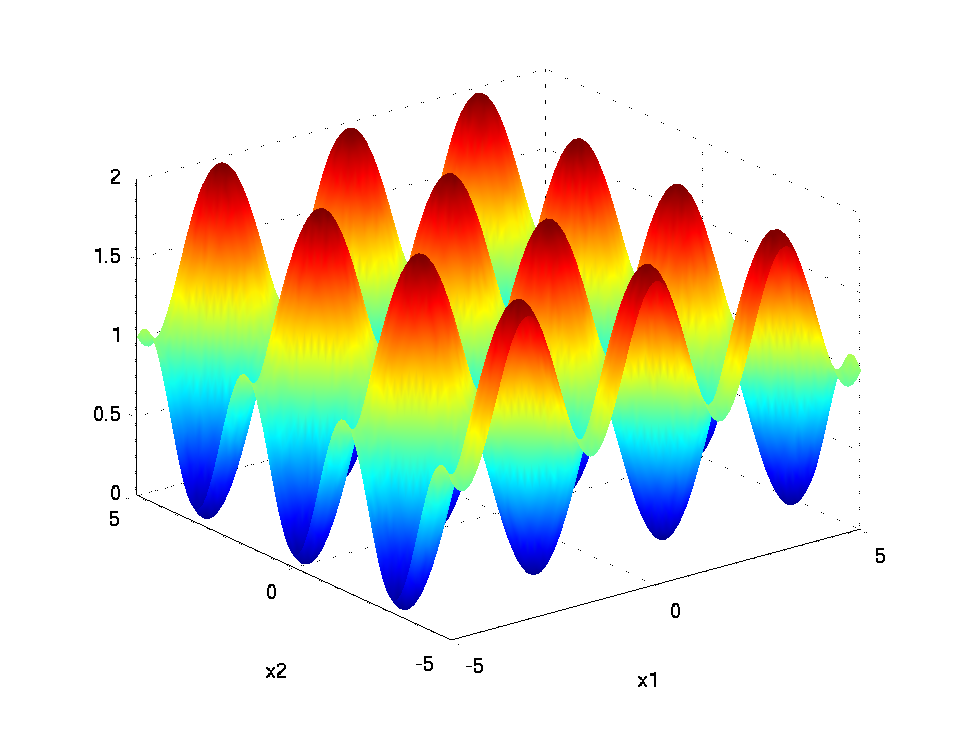
\includegraphics[width=0.7\columnwidth]{figs/global_opt2.eps}
\end{center}
Hér er erfiðara að koma auga á hámarkið, en við finnum það m.þ.a. leysa 
\[\nabla f(x_1,x_2)=\left(\frac{\partial f}{\partial x_1},\frac{\partial f}{\partial x_2}\right)=\vec{0}\]
þ.e.
\begin{eqnarray*}
\frac{\partial f}{\partial x_1}=&2\cos(x_1)\left(-\sin(x_1)\right)=0 &\Rightarrow x_1=k\frac{\pi}{2},\;k\in\mathbb{Z}\\
\frac{\partial f}{\partial x_2}=&2\sin(x_2)\cos(x_2)=0 &\Rightarrow x_2=k\frac{\pi}{2},\;k\in\mathbb{Z}
\end{eqnarray*}
Athugum að einnig þarf að gilda $-5\leq k\frac{\pi}{2}\leq 5$. Skoðum tilsvarandi gildi á $f(x_1,x_2)$.
\end{lausnSYND}

Víðvær bestun er erfið vegna þess að almennt er erfitt að finna allar núllstöðvar $\nabla f$. Einnig er til í dæminu að $\nabla f$ sé hreinlega óskilgreint (ódiffranleg bestun) sem flækir málið ennfrekar.

Nálgunaraðferðir eins og t.d. \emph{sub-tour reversal} finna iðulega staðbundin há-/lággildi.

\begin{center}
  \includegraphics[width=0.5\columnwidth]{figs/global_approx.eps}
\end{center}

\section{Hermd kólnun}
\ath{Hermd kólnun} (e. simulated annealing) er algeng lausnaraðferð til að leysa víðværa bestun.
\begin{enumerate}
  \item Byrja með einhverja gjaldgenga lausn.
  \item Ítra:
  \begin{enumerate}
    \item Næsta lausn er valin af handahófi úr þeim lausnum sem eru \emph{nálægt} núverandi lausn. Hver þeirra verður fyrir valinu ræðst af líkindadreifingu sem ákvarðast af mismuni markfallsgilda ásamt \emph{hitastigi} ($T$) sem lækkar smám saman þegar ítrunum fjölgar.
    \item Af og til samþykkjum við lausnir sem eru \emph{verri} en sú besta sem fundist hefur fram að þessu. Tilgangur með því er að draga úr líkum á því að festa í staðbundnu lággildi.
    \subitem Þegar hitastigið ($T$) er hátt eru miklar líkur á að samþykkja verri lausn. Þegar það er lágt eru líkurnar litlar.
  \end{enumerate}
  \begin{aths}Analógía með kólnun á bráðnu gleri eða málmi:
  \begin{eqnarray*} \mbox{Bráðið kvartz}  & \begin{tabular}{cp{9cm}} 
    $\nearrow$ & Hröð kólnun: hrafntinna (óregluleg kristallsb.) \\
    $\searrow$ & Hæg kólnun: gler (regluleg kristallsbygging) \end{tabular}\\ &  \Rightarrow \mbox{lægri stöðuorka $\Rightarrow$ víðvært lágmark}\end{eqnarray*}
  \end{aths}
  Látum
  \begin{center}\begin{tabular}{lr}
    $z_c$ & markfall núverandi lausnar \\
    $z_n$ & markfall kandídats lausnar
  \end{tabular}\end{center}

  Samþykkjum kandídat ef $z_n\geq z_c$ (því hann er betri -- g.r.f. hámörkunarverkefni). Ef $z_n<z_c$ samþykkjum við kandídat með líkum
 \[ Pr\{\mbox{samþykkja}\}=e^{(z_n-z_c)/T} \]
\begin{aths}$\lim_{T\to0} e^{(z_n-z_c)/T}=0$ því $(z_n-z_c)<0$.\end{aths}
\end{enumerate}

\begin{samepage}
\subsection*{Dæmi um stöðvunarskilyrði}
\begin{enumerate}
  \item ákveðinn fjöldi ítrana hefur verið náð,
  \item hitastig náð einhverju tilteknu gildi,
  \item engin bæting á markfalli fundist í langan tíma.
\end{enumerate}
\end{samepage}

Þegar leit lýkur vitum við ekki hversu langt lausnin okkar er frá besta gildi (gætum jafnvel hafa slysast á þá bestu).

Sérsníða þarf reiknirit sem byggja á hermdri kólnun að sérhverri tegund verkefna. Það sama gildir um \ath{bannleit} (e. tabu-search 13.2 í H\&L) og \ath{erfðaalgrím} (e. genetic algorithms í 13.4 í H\&L).

\begin{lausn}[Nálgunarlausn á TSP \ref{daemi:tsp} fundið með hermdri kólnun]\hspace{.1cm}
  \begin{enumerate}
    \item Byrjum með einhverja sæmilega góða upphafslausn, t.d. $1\to2\to3\to4\to5\to6\to7\to1$, með $z_c=69$.
      \subitem Oft fæst þokkaleg upphafslausn með því að velja upphafspunkt af handahófi. Förum næst í þann punkt sem er í stystu fjarlægð frá upphafspunktinum og svo koll af kolli (gráðug aðferð).
    \item Notum \emph{sub-tour reversal} t.þ.a. finna lausnir í nágrenni núverandi lausnar.
      \subitem Veljum upphafs- og endapunkt af handahófi t.d. $1\to2\to3\to5\to4\to6\to7\to1$. Kandídatinn er gjaldgengur með $z_n=65$. 	\subsubitem Þar sem $z_n=65<69=z_c$ samþykkjum við $1\to2\to3\to5\to4\to6\to7\to1$ sem bestu lausn.
      \subsubitem Ef hins vegar $z_n>z_c$ þá er nýja lausnin verri. Samþykkjum hana með líkum $\exp\left\{\left(z_c-z_n\right)/T\right\}$.
    \item Hitastýring: Í upphafi má t.d. nota $T_1=0.2z_c$ og síðan $T_k=0.95T_{k-1}$, $k=2,3,4,...$
  \end{enumerate}

\end{lausn}



\backmatter

\include{bibliography}  % include bibliography

% unix: makeindex showgirls.idx 
\printindex

\end{document}
